% nie rusza�
\RequirePackage{ifpdf}
\newif\ifelektroniczna
\newif\ifjednostronna
\newif\ifprojektInzynierski

%%%%%%%%%%%%%%%%%%%%%%%%%%%%%%%%%%%%%%%%%%%%%%%%%%%%%%%%%%%%%%%%%%%%%%%%%%%%
% USTAWIENIA GLOBALNE I domy�lna �cie�ka do plik�w z obrazkami, kodowanie itp. 
% okre�lone s� w drugiej sekcji ustawie�

% czy projekt czy praca magisterska
%\projektInzynierskitrue % projekt
\projektInzynierskifalse % praca magisterska

% czy wersja elektroniczna (pdf z kolorowymi linkami) czy nie (np. do druku)
\elektronicznatrue
%\elektronicznafalse

% czy jednostronna (recenzent), czy dwustronna (do akt);
% UWAGA: to nie jest dyrektywa dla drukarki; nie zmienia sposobu wydruku, 
% tylko to, w jaki spos�b rozpoczynane s� rozdzia�y, ustawiane marginesy
% itp.

%\jednostronnafalse
\jednostronnatrue

%%%%%%%%%%%%%%%%%%%%%%%%%%%%%%%%%%%%%%%%%%%%%%%%%%%%%%%%%%%%%%%%%%%%%%%%%%%%


% nie rusza�
\ifjednostronna
    \def\strony{oneside,openany}
\else
    \def\strony{twoside,openright}
\fi

\ifpdf
    % uwaga, ustawiaj�c co� innego ni� 12 sprawd� uk�ad strony tytu�owej (marginesy)
    \documentclass[pdftex,12pt,a4paper,\strony,colorlinks,nocenter,noupper,crosshair]{thesis}
    \usepackage[pdftex]{graphicx}
    \pdfcompresslevel=1
\else    
    \documentclass[12pt,a4paper,\strony,nocenter,noupper,crosshair]{thesis}
    \usepackage{graphicx}
\fi

% nie rusza�
\usepackage{url}
\usepackage{stronatytulowa}

%%%%%%%%%%%%%%%%%%%%%%%%%%%%%%%%%%%%%%%%%%%%%%%%%%%%%%%%%%%%%%%%%%%%%%%%%%%%
% USTAWIENIA GLOBALNE - cz�� 2
%

% kodowanie dokumentu
%\usepackage[utf8]{inputenc}   % linuks/windows/mac; pozwala na �atwe mieszanie znak�w z r�nych j�zyk�w
\usepackage[cp1250]{inputenc} % windows

% dane 
\ifprojektInzynierski
    \def\rodzaj{Projekt in�ynierski}
\else
    \def\rodzaj{Praca dyplomowa magisterska}
\fi
%\def\rodzaj{Praca przej�ciowa}

% stan na 2011-2012
\ifprojektInzynierski
    \def\wydzial{In�ynierii Biomedycznej}
\else
    \def\wydzial{In�ynierii Biomedycznej}
\fi

\def\tytul{TYTUL \\PRACY} % Prosz� u�y� i ma�ych, i du�ych liter!
\def\autor{Autor: Anna Ku�acz} %Jan Kowalski a NIE JAN KOWALSKI

% tytu� i autor dla pdfa - najcz�ciej jw, ale bez podzia�u na liniie i BEZ POLSKICH LITER
\def\tytulpdf{TYTUL DLA PDFa}
\def\autorpdf{AUTOR DLA PDFa}

% promotor
\def\promotor{Kieruj�cy prac�: dr Barbara Mika} % prof. nzw. dr hab. in�. dr n.med doc. Jan Kowalski

% z konsultantem/bez konsultanta
%\def\konsultant{Konsultant: Konsultant} prof. nzw. dr hab. in�. dr n.med doc. Jan Nowak
\def\konsultant{}

\def\data{Zabrze, marzec, 2020} % uwaga na wielko�� liter: grudzie� 2012/czerwiec 2012/..

% do pdfa
\def\slowakluczowe{SLOWA,KLUCZOWE}

% �cie�ka do obrazk�w
\graphicspath{{./rysunki/}}

% ustawienia dla pdfa
\ifpdf
\ifelektroniczna
     \usepackage[pdfusetitle=true,
	  pdfsubject={\tytulpdf},
	        pdfkeywords={\slowakluczowe}, 
		pdfcreator={\autorpdf},
		pdfstartview=FitV,
		linkcolor=blue,
		citecolor=red,
		]{hyperref}
\fi                 
\fi


\usepackage{layout}% poka� marginesy

% Nazwa za��cznik�w 
\def\appendixname{Za��cznik}
%%%%%%%%%%%%%%%%%%%%%%%%%%%%%%%%%%%%%%%%%%%%%%%%%%%%%%%%%%%%%%%%%%%%%%%%%%%%

% nie rusza� (cho� chwilowo niepotrzebne)
%	\author{\autor}
%	\title{\tytul}
%	\date{\data}
%

% === PAKIETY ===

% �adne czcionki dla PDF + ustawienia spolszczaj�ce
\usepackage{t1enc,amsmath}
\usepackage[OT4,plmath]{polski}

% potrzebne dla strony tytu�owej:
\usepackage{helvet} 

% pierwszy paragraf w rozdziale/sekcji powinien by� wci�ty
\usepackage{indentfirst}

% marginesy
%\usepackage{anysize}
%\marginsize{3cm}{2.5cm}{2.5cm}{2.5cm}%LPGD
%\setlength{\textheight}{24cm}
% za spraw� thesis
%\textwidth 150mm
%\textheight 225mm

% czcionki matematyczne
\usepackage{amsfonts}

% rysunki z�o�one z wielu [pod]rysunk�w
\usepackage{subfig}
\captionsetup[subfigure]{justification=centerfirst}

% mo�liwo�� sklejania wierszy tabeli
\usepackage{multirow}

% mo�liwo�� wklejania adres�w - jest ju� w��czony wy�ej
%\usepackage{url}

% ulepszona obs�uga cytowa�
\usepackage{cite}

% listingi
\usepackage{listings}
% domy�lne ustawienia (niestety utf8 nie jest akceptowany)
%\lstset{language={Matlab},inputencoding=cp1250}}
%\lstset{language={Matlab},inputencoding=latin2}}
\lstset{language={Java},inputencoding=latin2} % powinno pasowa� te� do C#

% \addcontentsline nie dzia�a za dobrze w po��czeniu z hyperref, ale to nie dzia�a z klas� thesis
%\usepackage[nottoc]{tocbibind}

% strona po cleardoublepage powinna by� pusta, nie z nag��wkami
\usepackage{cleardpempty}

% == opcjonalne

% wymu� po�o�enie grafiki (itp.) przez [H]
\usepackage{float} 

% znak promila i inne znaki specjalne
%\usepackage{textcomp}

% je�li trzeba obr�ci� stron� (wstawi� co� w orientacji poziomej), u�yj tych pakiet�w
%\ifpdf\usepackage{pdflscape}\else\usepackage{lscape}\fi

% je�li potrzebujesz d�ugich tabeli (wiele stron)
\usepackage{longtable}

% === POLECENIA DODATKOWE ===

% wektor w tek�cie
\def\vec#1{\ensuremath{\mathbf{#1}}}

% anglicyzmy i �acinizmy
\def\ang#1{ang.~\emph{#1}}
\def\lat#1{�ac.~\emph{#1}}

% proste e (jako podstawa logarytmu naturalnego) we wzorach i w tek�cie:
\def\e{\ensuremath{\textrm{\normalfont{}e}}}

% znak stopnia [jak w "5 stopni"]
\def\stopien{\ensuremath{^{\circ}}\protect\space}

% notatki na marginesie
\def\fixme#1{\marginpar{\tiny{}#1}}
%\def\fixme#1{} % gdy nie chcemy ich drukowa�, wystarczy zast�pi� powy�sze tym

%ODNOSNIKI 
% �eby wykorzysta� przypis dwukrotnie; druga wersja gorzej dzia�a�a w po��czeniu 
% z hyperref; czyli \footnote{blablabla \label{przypisX}} + \footnotereuse{przypisX}
%\newcommand{\footnreuse}[1]{\raisebox{1ex}{\scriptsize{}\protect\ref{#1}}}

% == �RODOWISKA DLA TWIERDZE�, LEMAT�W itp. ===
\newtheorem{twierdzenie}{Twierdzenie}[chapter]
\newtheorem{wlasnosc}{W�asno��}[chapter]
\newtheorem{lemat}{Lemat}[chapter]
\newenvironment{dowod}{\parindent=0pt{\bf Dow�d. }}{\begin{flushright}$\square$\end{flushright}}

% === RACZEJ NIE RUSZA� ===

%\usepackage{makeidx}
%\makeindex
%\usepackage{threeparttable}
%\usepackage[small,center]{caption2}

\def\captionlabeldelim{.}

%\usepackage{geometry}
%GATHER{thesis.bib}
%\usepackage[twoside]{geometry}
%\geometry{ lmargin=3.5cm, rmargin=2.5cm, tmargin=3cm, bmargin=3cm,
%headheight=1cm, headsep=0.5cm, footskip=0pt }

\linespread{1}
\chapterfont{\Huge\bfseries}
\sectionfont{\bfseries\Large}
\subsectionfont{\bfseries\large}
\institutionfont{\bfseries}%\mdseries}
\def\captionlabelfont{\bfseries}

\renewcommand{\figureshortname}{Rys.}
\renewcommand{\tableshortname}{Tab.}

\renewcommand\floatpagefraction{.9}
\renewcommand\topfraction{.9}
\renewcommand\bottomfraction{.9}
\renewcommand\textfraction{.1}
\setcounter{totalnumber}{50}
\setcounter{topnumber}{50}
\setcounter{bottomnumber}{50}

\newcommand{\topcaption}{%                  % robi podpis nad tabelk� z odst�pem po podpisie
   \setlength{\abovecaptionskip}{0pt}%
   \setlength{\belowcaptionskip}{10pt}%
   \caption}


\usepackage{color}
% marginesy
\usepackage{anysize}
\marginsize{3cm}{2.5cm}{2.5cm}{2.5cm}%LPGD
%\setlength{\textheight}{24cm}
% za spraw� thesis
%\textwidth 150mm
%\textheight 225mm

\begin{document}
%
\bibliographystyle{acm}
%

%
%\stronatytulowa
\titlepage
%\ \cleardoublepage % je�li dwustronnie, to druga strona powinna by� pusta
\frontmatter 
%\maketitle

%\tocbibname

\tableofcontents \listoffigures \listoftables
%\listofacros
%\input{abbrev_body}
%\newpage
%\input{spis_oznaczen}

\mainmatter % <--- to + frontmatter powy�ej odpowiada za fakt, �e numerowanie jest od 1!
\chapter{Wst�p}
% \setlength{\parindent}{50pt} tak~si� robi wci�cia
% \indent akapit

W~pracy przedstawiono model, kt�ry opisuje odpowied� uk�adu immunologicznego na~rozwijaj�cy si� w~organizmie nowotw�r. Model ten~oparty jest na~modelu de~Pillis \cite{19}. Obejmuje on rozw�j kom�rek nowotworowych w~organizmie oraz~odpowied� kom�rek uk�adu immunologicznego w~tym, tak~zwanych ,,naturalnych zab�jc�w'' (ang. Natural Killer cells (NK)), limfocyt�w $T_{CD8+}$ oraz~limfocyt�w kr���cych.
W~pracy model ten zosta� poddany modyfikacji (w~oparciu o model de~Pillis \cite{19}) polegaj�cej na~uwzgl�dnieniu procesu leczenia nowotworu skojarzonymi metodami chemioterapii (z u�yciem leku cytostatycznego) oraz~immunoterapii z~u�yciem pewnej grupy cytokin\footnote{Cytokiny -- bia�ka o~niskiej masie cz�steczkowej bior�ce udzia� w~przekazywaniu informacji pomi�dzy kom�rkami; odgrywaj� istotn� rol� w~odpowiedzi zapalnej, apoptozie, wzro�cie i~r�nicowaniu kom�rek \cite{16}.}, tj. interleukin-2 (IL-2) oraz~limfocyt�w naciekaj�cych nowotw�r TIL (ang. Tumor-Infiltrating Lymphocytes\footnote{Limfocyty naciekaj�ce nowotw�r TIL - pewien rodzaj kom�rek uk�adu immunologicznego, kt�re przedostaj� si� z~krwi do nowotworu pacjenta; limfocyty te potrafi� rozpoznawa� i niszczy� kom�rki nowotworowe; w~terapii nowotworowej, limfocyty TIL s� pobierane z guza pacjenta, nast�pnie namna�ane w laboratorium i przetaczane ponownie do organizmu pacjenta w celu wzmocnienia jego uk�adu odporno�ciowego \cite{41}.}).

\section{Cel pracy}
Celem pracy by�o:
\begin{itemize}
\item zaimplementowaie modelu rozwoju nowotworu w~organizmie z~uwzgl�dnieniem leczenia skojarzonymi metodami chemioterapii i~immunoterapii,
\item przeprowadzenie symulacji leczenia nowotworu metod� chemioterapii, immunoterapii oraz~skojarzonymi metodami chemioterapii i~immunoterapii,
\item analiza rozwi�za� modelu nieuwzgl�dniaj�cego leczenia (dla zmian pocz�tkowej liczby kom�rek nowotworowych oraz limfocyt�w kr���cych),
\item analiza rozwi�za� modelu opisuj�cego leczenie wy��cznie metod� chemioterapii (dla zmian d�ugo�ci cyklu, dawki dozowanego cytostatyka, liczby powt�rze� cyklu oraz dnia rozpocz�cia chemioterapii),
\item analiza rozwi�za� modelu opisuj�cego leczenie wy��cznie metod� immunoterapii (dla zmian pocz�tkowej liczby kom�rek nowotworowych, dawki IL-2, dawki TIL, liczby powt�rze� cyklu IL-2 oraz dnia rozpocz�cia immunoterapii),
\item analiza rozwi�za� modelu opisuj�cego leczenie zar�wno metod� chemioterapii, jak~i~immunoterapii (dla zmian warunk�w pocz�tkowych chemioterapii, warunk�w pocz�tkowych immunoterapii, kolejno�ci wdro�enia poszczeg�lnych terapii oraz dla pacjent�w o r�nej kondycji uk�ad�w immunologicznych).
\end{itemize}

\section{Uk�ad pracy}
Praca sk�ada si� z~nast�puj�cych cz�ci:
\begin{itemize}
\item wst�pu teoretycznego zawieraj�cego informacje na~temat rodzaj�w nowotwor�w i~sposob�w ich rozwoju oraz~niekt�rych metod ich leczenia, a~tak�e dotycz�cych budowy i~sposobu dzia�ania uk�adu immunologicznego,
\item przedstawienia zaimplementowanego modelu, na~kt�rym przeprowadzano symulacje (za�o�e�, r�wna�, opisu, parametr�w),
\item opisu dokonanych symulacji i~scenariuszy, wed�ug kt�rych zosta�y przeprowadzone,
\item analizy wynik�w symulacji i~wynikaj�cych z~nich wniosk�w,
\item podsumowania oraz perspektyw rozwoju niniejszej pracy.
\end{itemize}

\chapter{Wprowadzenie teoretyczne}
\section{Procesy nowotworowe}
Nowotworem okre�la si� nieprawid�owe kom�rki w~organizmie, kt�rych wzrost odbywa si� w~spos�b niekontrolowany \cite{1, 2}. Czasami (najcz�ciej w~przypadku zmian zapalnych) naprzemiennie z~poj�ciem nowotw�r, stosowane jest okre�lenie guz \cite{24}. W~zdrowym organizmie wyst�puje r�wnowaga pomi�dzy tempem podzia��w kom�rek a~ich obumieraniem. W~przypadku nowotworu ginie mniej kom�rek ni�~przybywa \cite{3}. W~efekcie spontanicznej proliferacji kom�rek nowotworowych sk�adaj�ca si� z~nich struktura zaczyna niszczy� narz�d, w~kt�rym wyst�pi� proces nowotworowy. Niekt�re z~kom�rek nowotworowych mog� oderwa� si� od~pozosta�ych, przedosta� si� do~naczy� krwiono�nych i~limfatycznych, a~w~konsekwencji dawa� przerzuty do~innych narz�d�w \cite {2}. Powstawanie nowotworu wi��e si� z~wieloma zmianami materia�u genetycznego. Rozpocz�cie tego procesu zale�y zar�wno od~wielko�ci zmiany, jak~i~miejsca, w~kt�rym wyst�pi�a\cite{3}. 

Transformacja kom�rkowa oznacza wielostopniowy proces, podczas kt�rego na~ka�dym etapie zachodz� zmiany genetyczne prowadz�ce do~zaburze� wzrostu kom�rek prawid�owych\cite{24}.

Na~powierzchni kom�rek nowotworowych pojawiaj� si� zmienione albo~obce antygeny, natomiast zanikaj� cz�steczki charakterystyczne dla~kom�rek w�asnych organizmu. Zmiany te,~zazwyczaj s�~rozpoznawane przez~uk�ad odporno�ciowy, co~umo�liwia skuteczn� walk� z~kom�rkami nowotworowymi. Jednak rozwojowi nowotworu cz�sto towarzyszy aktywacja r�nych mechanizm�w maskuj�cych obecno�� kom�rek z�o�liwie transformowanych, kt�re powoduj�, �e kom�rki te staj� si� ,,niewidoczne'' dla~uk�adu immunologicznego. Na~tych mechanizmach maskuj�cych skupia si� immunoterapia, kt�ra jest~jednym ze~sposob�w leczenia nowotwor�w\cite{31}.

Jedn� z~g��wnych przyczyn wyst�powania proces�w nowotworowych, s� pojawiaj�ce si� zmiany genetyczne zwi�zane z~r�nymi zmianami fizjologicznymi zachodz�cymi w~kom�rce, w~szczeg�lno�ci z~\cite{24}:
\begin{itemize}
\item samowystarczalno�ci� w~wytwarzaniu sygna��w do~wzrostu,
\item niewra�liwo�ci� na~inhibitory sygna��w wzrostu,
\item unikaniem programowanej �mierci,
\item nieograniczonym potencja�em replikacyjnym, 
\item podtrzymywaniem angiogenezy,
\item inwazj� tkankow�,
\item przerzutami,
\item unikaniem destrukcji immunologicznej.
\end{itemize} 

Opr�cz wy�ej wymienionych zmian zachodz�cych w kom�rce, warto tak�e~zwr�ci� uwag� na~zmiany system�w naprawy DNA oraz~zmiany system�w reguluj�cych podstawowe procesy kom�rkowe (na przyk�ad wzrost, r�nicowanie, apoptoz�\footnote{Apoptoza -- �mier� programowana, �mier� samob�jcza kom�rki zachodz�ca w~warunkach fizjologicznych \cite{12}.}). Na~skutek modyfikacji system�w naprawczych dochodzi do~szybkiej i~du�ej niestabilno�ci genomu. Zmiany w~systemach reguluj�cych, powoduj� z kolei, powolny proces zaburzenia homeostazy kom�rki oraz~stopniowo narastaj�c� niestabilno�� genomu. Choroby nowotworowe w~wi�kszo�ci rozwijaj� si� na~skutek zmian w~systemach reguluj�cych, dlatego od~pojawienia si� pocz�tkowej zmiany do~klinicznego wykrycia guza mija zazwyczaj wiele lat\cite{3}.

Mechanizmy genetyczne, le��ce u~podstaw wy�ej wymienionych zmian fizjologicznych, mog� r�ni� si� dla~poszczeg�lnych nowotwor�w, jednak to w�a�nie zmiany fizjologiczne~s�~wsp�lne dla~wi�kszo�ci nowotwor�w i~to~one~odpowiadaj� zar�wno za~prze�ycie, jak~i~rozrost nowotworu\cite{24}. 

\newpage
\section{Budowa uk�adu immunologicznego i~jego znaczenie w~procesie leczenia nowotwor�w}
Na uk�ad immunologiczny sk�adaj� si� mechanizmy odporno�ci swoistej (nabytej), jak i~nieswoistej (wrodzonej) \cite{4,5,20}. Ich podzia� przedstawia Tab. \ref{r�nice_mi�dzy_nab_a_wrodz}. 

Mechanizmy odporno�ci nabytej s�~aktywowane, gdy~zawodz� mechanizmy odporno�ci wrodzonej, kt�re np. nie~zapobiegn� wnikaniu lub~nie~usun� patogenu \cite{20}. 

\begin{table}[!htb]
	\centering
	\caption{Mechanizmy obronne odporno�ci swoistej i~nieswoistej\cite{7}.}\label{r�nice_mi�dzy_nab_a_wrodz}
	\begin{tabular}{|l|l|l|p{0.35\linewidth}|} \cline{1-3} \cline{4-4} 
		\multicolumn{2}{|c|}{Odporno��} & Element uk�adu & Dzia�anie obronne \\
		\multicolumn{2}{|c|}{ } & immunologicznego & \\ \hline
		\multirow{2}{1cm}{Nieswoista (wrodzona)} & Humoralna & Lizozym & bakterioliza bakterii Gram dodatnich, liza bakterii Gram-ujemnych po~usuni�ciu warstwy liposacharydowej\\ \cline{3-4}
		& & Laktoferyna & pozbawienie bakterii dost�pu do~�elaza poprzez wi�zanie go~\\ \cline{3-4}
		& & Transferyna & pozbawienie bakterii dost�pu do~�elaza poprzez wi�zanie go~\\ \cline{3-4}
		& & Bia�ka ostrej fazy & aktywacja limfocyt�w, makrofag�w, dope�niacza na~drodze klasycznej \\ \cline{3-4}
		& & Dope�niacz & uaktywnienie uk�adu dope�niacza\\ \cline{3-4}
		& & Interferony & hamowanie transformacji limfocyt�w pod wp�ywem mitogen�w \\
		\cline{2-4}
		& Kom�rkowa & Fagocyty & fagocytoza\\ \cline{3-4}
		& & Eozynofile & produkcja prostoglandyn PGE1 i~PGE2, kt�re hamuj� uwalnianie mediator�w przez~kom�rki tuczne i~bazofile \\ \cline{3-4}
		& & Kom�rki K & cytotoksyczno�� zale�na od~przeciwcia�\\ \cline{3-4}
		& & Kom�rki NK & spontaniczne niszczenie kom�rek zaka�onych wirusem\\ \hline \cline{3-4}
		\multirow{2}{3cm}{Swoista (nabyta)} & Humoralna & Immunoglobuliny \\ \cline{3-3}
		& & Limfocyty typu B \\
		\cline{2-3}
		& Kom�rkowa & Limfocyty typu T \\ \cline{1-3}
		\end{tabular}
\end{table}

Zasadnicze znaczenie w~odporno�ci organizmu maj� sk�ra, b�ony �luzowe, fagocyty, limfocyty typu T i~B\footnote{Limfocyty typu B -- wyspecjalizowane kom�rki uk�adu immunologicznego, kt�rych g��wna funkcja to~wytwarzanie przeciwcia�\cite{28}.}, kom�rki NK, przeciwcia�a oraz~uk�ad dope�niacza\cite{28}.

Uk�ad dope�niacza (komplement) tworzy grupa oko�o 40 bia�ek, kt�re zabezpieczaj� organizm przed~atakiem drobnoustroj�w. Wspiera on mechanizmy wrodzonej odporno�ci immunologicznej przez:~zabijanie drobnoustroj�w za~po�rednictwem lizy, chemotaksj� kom�rek fagocytarnych oraz~u�atwianie procesu fagocytozy. Komplement aktywowany jest kaskadowo (ka�dy kolejny sk�adnik aktywuje nast�pny). \newline \newline Mo�na wyr�ni� trzy drogi aktywacji dope�niacza\cite{13}:

\begin{itemize}
\item klasyczn�,
\item alternatywn�,
\item lektynow�.
\end{itemize} 

Klasyczna droga aktywacji \label{klasyk} komplementu zachodzi z~udzia�em swoistych immunoglobulin, kt�re zwi�zane s�~z~powierzchni� drobnoustroj�w. Prowadzi ona~do~�mierci litycznej kom�rki docelowej (bakterioliza).

Znacznie szybsza jest droga alternatywna (properdynowa), poniewa� kszta�tuje si� ona~od~momentu wnikni�cia patogenu. W~tym~przypadku drobnoustroje ulegaj� spontanicznej opsonizacji\footnote{Opsonizacja -- proces u�atwiaj�cy fagocytoz� \cite{13}.} przez~cz�steczki C3b dope�niacza. U�atwia to~ich~poch�anianie przez~kom�rki fagocytarne.

Podczas lektynowej drogi aktywacji nast�puje po��czenie cz�steczki cukru obecnej na~powierzchni bakterii z~lektyn� wi���c� mannoz� MBL (ang. Mannose Binding Lectin). Ta~interakcja prowadzi do~rozk�adu czynnik�w C2 i~C4 uk�adu dope�niacza.

Alternatywna droga aktywacji uk�adu dope�niacza jest~podstawowym mechanizmem wrodzonego uk�adu odporno�ciowego. Organizm uruchamia kaskad� nieswoistych reakcji obronnych zanim pojawi� si� swoiste w~stosunku do~mikroorganizmu przeciwcia�a. Zapewnia to~oszcz�dno�� czasu, ale~alternatywna droga aktywacji oddzia�uje tak�e~na~w�asne tkanki, co~ogranicza sprawne funkcjonowanie wielu regulator�w \cite{13}. \newline \newline \indent Funkcjonowanie mechanizm�w nieswoistych jest niezale�ne od~wcze�niejszej styczno�ci organizmu z~czynnikami patogennymi i~pe�ni funkcj� obronn� przed~infekcjami i~chorobami b�d�cymi skutkiem dzia�ania czynnik�w �rodowiskowych. Mechanizmy te cechuje mniejsza precyzja, ale~s�~one zdolne do~szybkiego rozpoznawania i~niszczenia wnikaj�cych drobnoustroj�w. Odporno�� wrodzon� warunkuj� mi�dzy innymi: kom�rki NK, makrofagi, granulocyty oraz~monocyty \cite{4}.

Odporno�� swoista rozpoznaje antygeny\footnote{Antygeny -- zwi�zki wywo�uj�ce reakcje uk�adu immunologicznego; najcz�ciej substancje wielkocz�steczkowe, rozpoznawane swoi�cie poprzez powierzchniowe receptory limfocyt�w \cite{20}.} bardzo precyzyjnie. Jej wa�nymi elementami s�~limfocyty typu T, limfocyty typu B, cytokiny oraz~przeciwcia�a. Kom�rki te s�~zdolne do~wytwarzania nieograniczonej liczby receptor�w. Dodatkowo, je�li dojdzie do~ich kontaktu z~antygenem wytwarza si� pami�� immunologiczna \cite{4}, dzi�ki kt�rej przy~ponownym zetkni�ciu kom�rki danego typu z~odpowiednim antygenem wytwarzana odpowied� immunologiczna jest~szybsza i~silniejsza \cite{20}. W~przypadku limfocyt�w typu T, typ odpowiedzi swoistej okre�lany jest jako kom�rkowy (tj. zwi�zany z~aktywno�ci� kom�rek uk�adu immunologicznego \cite{13}), natomiast dla~ limfocyt�w typu B -- humoralny (tj. zwi�zany z~aktywno�ci� immunoglobulin \cite{13}). \newline

Do mechanizm�w swoistej odporno�ci nale�� \cite{6}:
\begin{itemize}
\item aktywno�� cytokin i~chemokin,
\item cytokinozale�na wrodzona oporno�� leukocyt�w i~innych kom�rek,
\item zabijanie zaka�onych lub~nowotworowych kom�rek przez~kom�rki NK, komplement aktywowany lektynami lub~drog� alternatywn�,
\item opsonizacja i~fagocytoza\footnote{Fagocytoza -- usuwanie kompleks�w immunologicznych i~uszkodzonych kom�rek (u�atwienie fagocytozy immunologicznej). Efektywne niszczenie drobnoustroj�w przez~fagocyty \cite{13, 14}.}.
\end{itemize}

Pomimo bardzo du�ego znaczenia uk�adu immunologicznego dla~organizmu, wiele mechanizm�w jego dzia�ania pozostaje jeszcze niewyja�nionych \cite{4}. \newline \newline Znacz�c� rol� w~oddzia�ywaniu uk�adu immunologicznego na~rozwijaj�cy si� nowotw�r pe�ni�:

\begin{itemize}
\item kom�rki NK,
\item limfocyty $T_{CD8+}$,
\item interleukiny (IL).
\end{itemize}

W~zwi�zku z~wa�n� funkcj� wy�ej wymienionych kom�rek, uj�to je~w~opisywanym modelu, natomiast ich~biologiczne znaczenie opisano w~dalszej cz�ci pracy.

\subsection{Kom�rki NK}
Wa�n� rol� w~odpowiedzi immunologicznej pe�ni�~kom�rki NK (limfocyty NK), czyli limfocyty cytotoksyczne\cite{30} stanowi�ce populacj� odr�bn� od~limfocyt�w typu B~i~T\cite{7}. Limfocyty NK stanowi� oko�o 10\% limfocyt�w obecnych we~krwi \cite{5, 30, 31}. 
Kom�rki NK to~efektorowe kom�rki cytotoksyczne b�d�ce elementem odporno�ci nieswoistej organizmu. S�~to du�e kom�rki limfoidalne posiadaj�ce umiej�tno�� rozpoznawania wielu konfiguracji molekularnych wyst�puj�cych m.in. na~powierzchni kom�rek w�asnych, zaka�onych wirusem oraz~nowotworowych\cite{29}.
Ich~g��wnym zadaniem jest~niszczenie kom�rek nowotworowych i~zainfekowanych wirusami \cite{5}. 

Kom�rki NK s�~szybkie i~skuteczne w~dzia�aniu\cite{31}. Limfocyty NK identyfikowane s�~poprzez ekspresj� antygenu powierzchniowego CD56 i~jednoczesny brak ekspresji antygenu CD3, a~tak�e ekspresj� receptor�w CD16, CD56 oraz~CD57.
\newpage
 Na~podstawie ekspresji receptora CD56 mo�na wyr�ni� dwie subpopulacje kom�rek NK\cite{31, 32}:
\begin{itemize}
\item subpopulacj� kom�rek $NK_{CD56^{bright}CD16^-}$ o~du�ej ekspresji receptora CD56 i~braku ekspresji receptora CD16, kt�re wytwarzaj� du�� ilo�� cytokin i~wyst�puj� g��wnie w~tkankach zmienionych chorobowo oraz~w�z�ach ch�onnych,
\item subpopulacj� kom�rek $NK_{CD56^{dim}CD16^+}$ o~umiarkowanej ekspresji receptora CD56 oraz~znacznej ekspresji receptora CD16, kt�re charakteryzuj� si� wysok� cytotoksyczno�ci� i~wyst�puj� g��wnie we~krwi obwodowej.
\end{itemize}

Istniej� liczne efektorowe mechanizmy cytotoksyczno�ci s�u��ce kom�rkom NK do~zabijania kom�rek zaka�onych przez~wirusy lub~kom�rek nowotworowych. Mechanizmy cytotoksyczno�ci podzielono na~cytotoksyczno�� zale�n� od~ziaren cytolitycznych i~cytotoksyczno�� zale�n� od~receptor�w dla~cz�steczek z~rodziny czynnika martwicy guza TNF (ang. Tumor Necrosis Factor). Kom�rki NK s�~aktywowane, gdy~kom�rki docelowe wykazuj� ekspresj� ligand�w wi���cych si� do~receptor�w kom�rek NK\cite{29}. \newline \newline \indent Kom�rki NK mog� wykazywa� ekspresj� r�nych receptor�w, np.\cite{29}:
\begin{itemize}
\item receptor�w naturalnej cytotoksyczno�ci NCRs (ang. Natural Cytotoxicity Receptors),
\item lektyno-podobnych receptor�w,
\item receptor�w aktywuj�cych lub~hamuj�cych kom�rki NK.
\end{itemize} 

Zmiany nowotworowe kom�rek w�asnych organizmu mog� by� usuwane przez~limfocyty NK bezpo�rednio lub~po�rednio (z~udzia�em innych kom�rek immunokompetentnych). Do~mechanizm�w bezpo�rednich nale�y proces naturalnej cytotoksyczno�ci, cytotoksyczno�ci zale�nej od~przeciwcia� oraz~cytotoksyczno�ci indukowanej. W~mechanizmach po�rednich najwi�ksze znaczenie maj� interakcje dwukierunkowe kom�rek NK z~kom�rkami dendrytycznymi DC (ang. Dendritic Cells), limfocytami typu~B~i~T oraz~makrofagami. Uwalniane cytokiny b�d�ce skutkiem zachodz�cych interakcji, r�wnocze�nie mobilizuj� kom�rki bior�ce udzia� w~interakcji oraz~pobudzaj� je~do~efektywnego niszczenia kom�rek nowotworowych\cite{31}.

Charakterystyczn� cech� kom�rek NK jest brak marker�w czy~receptor�w antygenowych na~ich powierzchni.
Dzia�anie kom�rek NK opiera si� na~rozpoznawaniu przez~receptor pektynowy reszt cukrowych, co~umo�liwia im~cytotoksyczne zniszczenie kom�rki docelowej, mi�dzy innymi nowotworowej. Z~kolei receptor hamuj�cy kom�rki typu ,,zab�jcy'' KIR (ang. Killer cells Inhibitory Receptor) zmniejsza aktywno�� kom�rek NK w~sytuacji, gdy rozpoznaj� one prawid�owe kom�rki organizmu \cite{4}.

Aktywacja kom�rek NK zale�y od~wypadkowego dzia�ania receptor�w aktywuj�cych i~hamuj�cych. Pozwala to~unikn�� atakowania przez~kom�rki NK niezmienionych kom�rek w�asnego organizmu. G��wnymi regulatorami aktywno�ci kom�rek NK s�~cz�steczki MHC klasy I. Cz�steczki te~s�~obecne na~ka�dej j�drzastej kom�rce organizmu, dzi�ki czemu mo�liwe jest~rozpoznawanie zdrowych kom�rek. Obni�enie ekspresji cz�steczek MHC klasy I na~kom�rkach nowotworowych umo�liwia skierowanie przeciwko nim odpowiedzi kom�rek NK. R�wnocze�nie, kom�rka NK musi otrzyma� w�a�ciwy sygna� z~receptor�w aktywuj�cych, aby~docelowa kom�rka zosta�a zabita. Takimi receptorami w~organizmie ludzkim s�~cz�steczki: NKp30, NKp44, NKp46, CD16 oraz~receptory nale��ce do~nadrodziny KIR \cite{30}. Pobudzone kom�rki NK wywo�uj� liz� kom�rek nowotworowych lub~indukuj� ich~apoptoz� \cite{31}.

Z wiekiem aktywno�� kom�rek NK spada (ze wzgl�du na~zwi�kszon� liczb� receptor�w KIR \cite{5}), co~zwi�ksza ryzyko �mierci spowodowanej ci�k� infekcj�. Niekorzystnymi czynnikami maj�cymi wp�yw na~uk�ad kom�rek NK s�: stres, niska aktywno�� fizyczna oraz~dieta wysokot�uszczowa \cite{4}. Silna aktywno�� cytotoksyczna kom�rek NK mo�e by� uznana za~oznak� dobrego zdrowia \cite{5}.

\subsection{Limfocyty typu T}
Jedn� z~grup limfocyt�w s�~limfocyty typu T, kt�re stanowi� odr�bny rodzaj kom�rek uk�adu immunologicznego. Limfocyty typu T wytwarzane s�~w~szpiku kostnym \cite{7}, a~na~wczesnym etapie �ycia p�odowego trafiaj� do~grasicy (limfocyty grasiczozale�ne), gdzie dojrzewaj�. Nast�pnie opuszczaj� grasic� i~przebywaj� w~r�nych narz�dach uk�adu odporno�ciowego, na~przyk�ad �ledzionie, w�z�ach ch�onnych, szpiku kostnym oraz~krwi obwodowej. Ich~wyspecjalizowan� funkcj� jest~bezpo�rednie atakowanie obcych antygen�w, na~przyk�ad wirus�w czy~grzyb�w. Pe�ni� tak�e~funkcj� regulatorow� w~obr�bie uk�adu immunologicznego \cite{28}. \newline \newline Limfocyty typu T oznaczane jako CD8+ dziel� si� na~limfocyty \cite{7}:
\begin{itemize}
\item cytotoksyczne $T_{c}$, kt�re odpowiadaj� za~niszczenie kom�rek i~odrzucanie przeszczep�w,
\item supresyjne $T_{s}$, kt�re odpowiadaj� za~hamowanie dzia�ania innych limfocyt�w, reakcji alergicznych i~utrzymanie tolerancji immunologicznej na~w�asne antygeny.
\end{itemize}

Rys. \ref{limfocyty_T_cd8+}, na~pomara�czowych, niebieskich i~r�owych polach przedstawia kolejne podzia�y limfocyt�w typu T wyst�puj�cych w~organizmie. Dodatkowo, na~polach szarych kr�tko opisano funkcj�, jak� one~pe�ni� lub~wymieniono ich~charakterystyczne cechy.

\begin{figure}[!h]
	\centering
	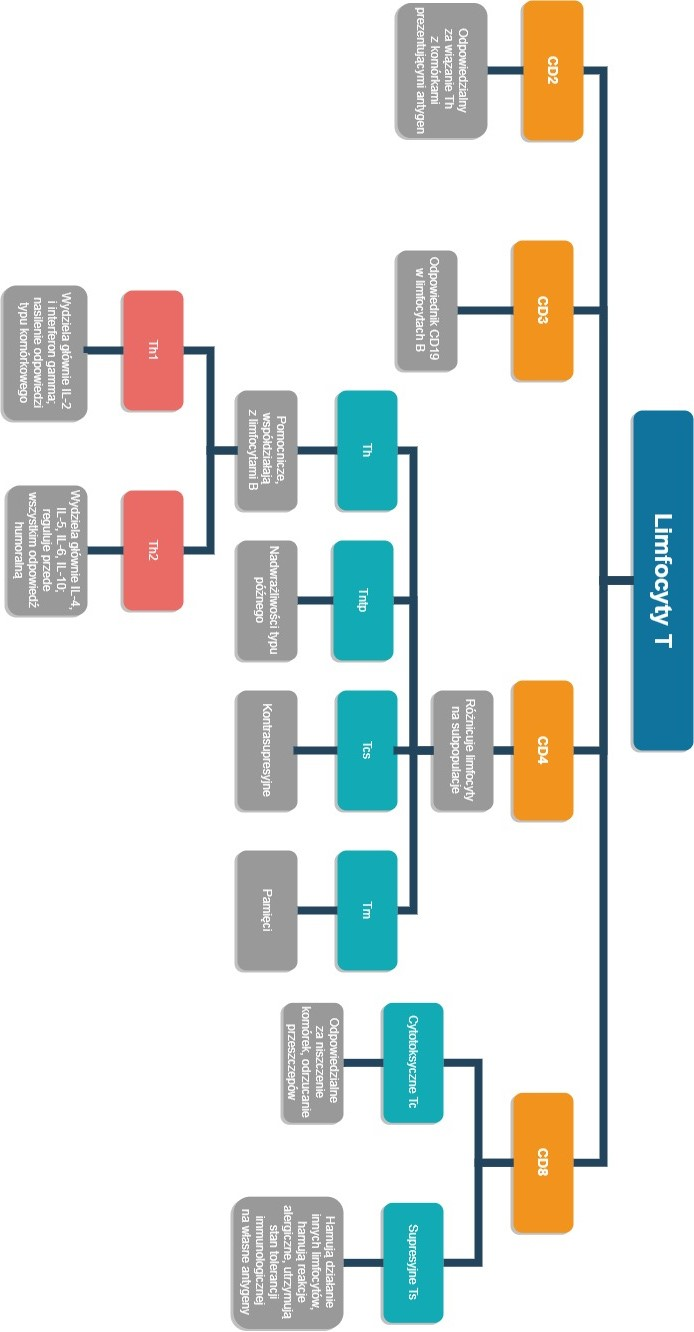
\includegraphics[width=0.7\textwidth, angle=180]{Limf_TT2}
	\caption{Podzia� (pola pomara�czowe, niebieskie i r�owe) oraz funkcje i cechy charakterystyczne (pola szare) limfocyt�w typu T \cite{7}.}\label{limfocyty_T_cd8+} 
\end{figure}

Podstaw� proces�w immunologicznych jest~prezentacja antygen�w przez~odpowiednie kom�rki pomocniczym limfocytom Th. Zwykle, kom�rkami prezentuj�cymi antygen APC (ang. Antigen Presenting Cells) s�~limfocyty typu B, kom�rki dendryczne oraz~makrofagi. Natomiast, pozosta�e kom�rki prezentuj�ce antygen to~limfocyty typu T, eozynofile, fibroblasty oraz~keranocyty \cite{7}.

Odpowied� immunologiczna swoista typu kom�rkowego, w~kt�r� zaanga�owane s�~subpopulacje limfocyt�w typu T, polega na~wywo�aniu reakcji zwalczania antygenu. Mo�liwe s�~dwa typy tej reakcji. W~pierwszym z~nich funkcj� efektor�w pe�ni� limfocyty CD4+, a~makrofagi s�~kom�rkami pomocniczymi. Drugi typ reakcji zak�ada, �e limfocyt cytotoksyczny CD8+ jest kom�rk� efektorow�, a~limfocyt CD4+ pomocnicz�.
Odporno�� kom�rkowa ma~za~zadanie, przede wszystkim walczy� z~zaka�eniami, ale~r�wnie� spe�nia wa�n� rol� w~reakcji kontaktowej ze zwi�zkami chemicznymi, w~odrzuceniu przeszczepu czy~tkanek zmienionych nowotworowo jak~r�wnie� w~niekt�rych reakcjach autoimmunologicznych \cite{4}.
Mi�dzy 5 a~6 dekad� �ycia ustaje czynno�� grasicy, czego skutkiem s�~zmiany w~subpopulacjach limfocyt�w typu T. Z~wiekiem g��wnie wzrasta liczba limfocyt�w CD4+, natomiast zmniejsza si� liczba limfocyt�w supresorowych i~cytotoksycznych CD8+ \cite{4}.

Kom�rki nowotworowe wsp�dzia�aj�c~z~makrofagami TAMs M2 powoduj� immunosupresj�\footnote{Immunosupresja -- stan charakteryzuj�cy si� os�abieniem b�d�~zahamowaniem odpowiedzi immunologicznej; dotyczy zar�wno odpowiedzi typu humoralnego, jak~i~kom�rkowego. Wi��e si� ze~zmiennymi niedoborami poszczeg�lnych klas przeciwcia� (IgG, IgM, IgA) oraz~spadkiem liczby i~dysfunkcj� kom�rek uk�adu odporno�ciowego, g��wnie limfocyt�w T, ujawniaj�c� si� zahamowaniem wytwarzania cytokin \cite{26}.} uk�adu immunologicznego. W~pocz�tkowym etapie choroby mo�na zaobserwowa� wzrost poziomu cytokin prozapalnych. Czynniki te~hamuj� cytotoksyczn� aktywno�� makrofag�w. Makrofagi TAMs M2 wydzielaj� zwi�zki o~dzia�aniu przeciwzapalnym, czego efektem jest~mi�dzy innymi indukcja limfocyt�w T regulatorowych ($T_{reg}$) oraz~supresja limfocyt�w $T_{CD8+}$ \cite{25}. Zwi�kszona ilo�� $T_{reg}$ hamuje aktywno�� kom�rek NK, $T_{CD4}+$ i~$T_{CD8+}$, co~przyczynia si� do~rozrostu nowotworu \cite{27}.

\subsection{Interleukiny}
Interleukiny s�~jedn� z~grup cytokin. S�u�� one, mi�dzy innymi, do~komunikacji pomi�dzy kom�rkami uk�adu odporno�ciowego. Interleukiny to~bia�ka produkowane g��wnie przez~leukocyty. 

Ze~wzgl�du na~cechy biologiczne, w~tym r�nice w~budowie molekularnej i~strukturze, interleukiny zosta�y zgrupowane w~trzy rodziny \cite{8}:
\begin{itemize}
\item pierwsz� -- podzielon� na~podrodzin� interleukiny-2 i~podrodzin� interferon�w (reprezentowan� przez~interferon-$\alpha$ (IFN-$\alpha$) i~interferon-$\beta$),
\item drug� -- rodzin� interleukiny-1,
\item trzeci� -- zawieraj�c� interleukin� 17A, B, C, D, F oraz~IL-8, 25 i~27, a~tak�e IL-31, 32 i~33. 
\end{itemize}

Najwi�ksze znaczenie w�r�d interleukin ma~IL-2, stymuluj�ca proliferacj� kom�rek NK i~wzmagaj�ca dzia�anie cytotoksyczne. Poza~IL-2, aktywno�� kom�rek NK jest~stymulowana r�wnie�~przez: IL-12, IL-18, IL-21, IFN-$\alpha$, IFN-$\beta$ oraz~IFN-$\gamma$. Kolejn� wa�n� interleukin� jest~IL-15, kt�ra jest odpowiedzialna za~r�nicowanie~i cytolityczn� aktywno�� dojrza�ych kom�rek NK. IL-15 ma~wp�yw na~w�a�ciwo�ci lityczne kom�rek NK i~mo�e mie� znaczenie w~immunoterapii nowotwor�w.

Bardzo istotna dla~odpowiedzi immunologicznej jest~interakcja kom�rek NK z~kom�rkami dendrytycznymi, kt�ra zale�y od~dzia�ania cytokin: IL-2, IL-12, IL-15, IL-18 oraz~IL-4. Cytokiny te~uwalniane s�~w~miejscu rozwoju odpowiedzi zapalnej zachodz�cej z~udzia�em kom�rek NK\cite{32}.

IL-2 i~IL-15 s�~najlepiej poznanymi naturalnymi stymulatorami kom�rek NK. Interleukiny te wzmacniaj� aktywno�� efektorow� oraz~pobudzaj� proliferacj� kom�rek NK. IL-2 stymuluje tak�e~regulatorowe i~pomocnicze limfocyty typu T. Natomiast IL-15 jest niezb�dnym czynnikiem w~utrzymaniu homeostazy kom�rek NK\cite{31}. \newline \newline \indent IL-2 zidentyfikowano po~raz~pierwszy jako~czynnik wzrostu TCGF kom�rek T (ang. T Cell Growth Factor). Najwa�niejszymi kom�rkami wytwarzaj�cymi IL-2 s�~limfocyty $T_{CD4+}$, niekt�re limfocyty $T_{CD8+}$ oraz~kom�rki NK aktywowane antygenem czy~mitogenem. IL-2 jest~produkowana tak�e~przez~kom�rki nowotworowe niekt�rych ch�oniak�w. IL-2 dzia�a endokrynnie na~kom�rki wykazuj�ce ekspresj� jej~receptora b�onowego oraz~autokrynnie na~kom�rki, kt�re j�~wytwarzaj�.
W~procesie odpowiedzi immunologicznej, IL-2 ma~za~zadanie modulowa� uk�ad immunologiczny oraz~bra�~udzia� w~mechanizmach odporno�ciowych w~przypadku zaka�e� i~nowotwor�w. 

IL-2 jest~podstawowym czynnikiem proliferacji kom�rek efektorowych: aktywowanych limfocyt�w typu T, limfocyt�w $T_{CD4+}$ i~limfocyt�w $T_{CD8+}$. Zwi�ksza ich~czas prze�ycia oraz~efektywno�� dzia�ania. Pod~wp�ywem IL-2 kom�rki NK s�~aktywowane i~stymulowane do~wydzielania szeregu cytokin. IL-2 oddzia�uje r�wnie�, po�rednio i~bezpo�rednio, na~inne kom�rki uk�adu odporno�ciowego, np.: limfocyty typu~B, makrofagi lub~monocyty\cite{34}.

IL-2, wytwarzana przez~limfocyty pomocnicze $T_{h1}$, wspomaga nabyt� odpowied� immunologiczn�, podtrzymuj�c proliferacj� i~zwi�kszaj�c aktywno�� limfocyt�w typu~$T_C$~i~B oraz~kom�rek~NK. Dodatkowo, jest~odpowiedzialna za~indukcj� apoptozy kom�rek aktywowanych i~pe�ni kluczow� rol� w~powstawaniu limfocyt�w regulatorowych typu~T ($T_{reg}$) oraz~utrzymywaniu ich~liczby w~organizmie. Bierze r�wnie�~udzia� w~regulacji odpowiedzi immunologicznej i~jej~wygaszaniu. IL-2 jest~niezb�dnym czynnikiem w~aktywacji i~pobudzeniu proliferacji cytotoksycznych limfocyt�w $T_{CD8+}$\cite{14}. \newline \newline \indent W~(,,Mo�liwo�ci wykorzystania kom�rek NK
w immunoterapii nowotwor�w'', Medycyna Og�lna i Nauki o Zdrowiu 2020, Tom 26, Nr 1, 8�16 \cite{31}) 1992~roku \textit{Agencja �ywno�ci i~lek�w} FDA (ang. Food and~Drug Administration) wyda�a zgod� na~zastosowanie IL-2 podczas leczenia raka nerki i~czerniaka, mimo~pojawiaj�cego~si� ryzyka ci�kiej toksyczno�ci mog�cej prowadzi� nawet do~zgonu. Ponadto, IL-2 wykazuje kr�tki okres p�trwania in~vivo oraz~mo�e~stymulowa� rozw�j nowotworu poprzez~utrzymanie pomocniczych limfocyt�w regulatorowych typu~T i~promowanie �mierci kom�rek indukowanej aktywacj� AICD (ang. Activation-Induced Cell Death) limfocyt�w efektorowych typu~T. 

Aby~zapobiec niepo��danym efektom, zaprojektowano IL-2 - ,,superkin�'' posiadaj�c� zwi�kszone powinowactwo do~IL-2R$\beta$. Dzi�ki~niej wspomagana~jest proliferacja limfocyt�w cytotoksycznych typu~T bez~wp�ywu na~liczb� limfocyt�w regulatorowych typu~T oraz~wzmocniona zostaje odpowied� przeciwnowotworowa. 

Obecnie testuje si� nisk� dawk� IL-2 w~formie monoterapii, jak~i~w~po��czeniu z~adaptywnym transferem kom�rek NK i~limfocyt�w typu~T jako~szczepionki. Badania\cite{31} potwierdzi�y tak�e~przeciwnowotworowe dzia�anie IL-15. Wykazano zwi�kszenie liczby kom�rek~NK i~limfocyt�w typu~T cytotoksycznych\cite{31}.

IL-6 jest~cytokin� o~znacz�cej roli w~rozwoju zespo�u wyniszczenia. Wytwarzana~jest przez~makrofagi, monocyty, fibroblasty, kom�rki �r�db�onka oraz~niekt�re kom�rki nowotworowe. IL-6 to~jeden z~najsilniejszych stymulator�w bia�ek ostrej fazy o~dzia�aniu prozapalnym. Jej~wzmo�one wytwarzanie wyst�puje podczas przebiegu licznych ostrych i~przewlek�ych zapale� oraz~w~obecno�ci nowotwor�w. Innymi prozapalnymi cytokinami~s�~m. in.: czynnik martwicy guza alfa TNF$_{\alpha}$, IL-1, IL-2, IFN-$\alpha$ oraz~IFN-$\gamma$\cite{3}. Warto wspomnie�, �e~IL-2, IL-6 i~interferony maj�~w�a�ciwo�ci depresjogenne\cite{21}.

\chapter{Leczenie nowotwor�w}

Leczenie pacjent�w onkologicznych, ma~na~celu osi�gni�cie najkorzystniejszego efektu przeciwnowotworowego, ale~tak�e zapewnienie choremu jak~najlepszej jako�ci �ycia. U~wielu pacjent�w wskutek choroby nowotworowej dochodzi do~pogorszenia kondycji zdrowotnej, a~jedn� z~najcz�stszych dolegliwo�ci jest~os�abienie, kt�re mo�e by� r�wnocze�nie podstawowym objawem zespo�u przewlek�ego zm�czenia (ZPZ). ZPZ jest~powodem ograniczenia codziennej aktywno�ci u~ponad 80\% \cite{38} pacjent�w z~nowotworami, u~kt�rych pojawiaj�ce si� objawy dotycz� nie~tylko sfery fizycznej, lecz~r�wnie� psychicznej i~socjalnej. ZPZ powoduje m. in. pogorszenie zdolno�ci koncentracji uwagi, pacjenci zmuszeni s�~do~ograniczenia lub~rezygnacji z~aktywno�ci zawodowej, co~pogarsza ich status ekonomiczny. Zazwyczaj chorzy nie~znajduj� zrozumienia w�r�d otoczenia, tak�e~w�r�d os�b sprawuj�cych nad~nimi specjalistyczn� opiek�. Wi�kszo�� onkolog�w (61\%\cite{38}) uwa�a, �e b�l towarzysz�cy chorobie nowotworowej jest~najwa�niejsz� dolegliwo�ci� u~chorych, podczas gdy wi�kszo�� pacjent�w (61\%\cite{38}) uwa�a os�abienie za~istotniejsz� dolegliwo��.

Pierwsze objawy ZPZ pojawiaj� si� najcz�ciej przy~rozpocz�ciu leczenia, jednak cz�sto wyst�puj� ju�~podczas bada� diagnostycznych. U~pacjent�w poddawanych chemioterapii objawy nasilaj� si� od~momentu do�ylnego podania cytoststyka, osi�gaj�c maksymalne nat�enie po~2-3 dniach, nast�pnie stopniowo si� zmniejszaj�. \newline \indent Ponad 30\% chorych odczuwa os�abienie nawet p� roku po~zako�czeniu chemioterapii, a~objawy ZPZ mog� utrzymywa� si� czasem nawet do~3 lat\cite{38}. 

\section{Chemioterapia}
Chemioterapia to~metoda leczenia, kt�ra polega na~niszczeniu kom�rek nowotworowych, drobnoustroj�w oraz~bakterii za~pomoc� �rodk�w chemicznych. W~przypadku nowotwor�w, stosuje si� r�ne grupy lek�w, tzw. cytostatyk�w. Zale�nie od~indywidualnych cech pacjenta chemioterapia ma~�ci�le okre�lony przebieg. Leki mog� by� stosowane w~monoterapii (stosowanie jednego leku cytostatycznego) lub~polichemioterapii (stosowanie kilku lek�w zgodnie z~okre�lonym schematem). Leki cytostatyczne podawane s�~w~sekwencjach co~kilka dni, tygodni lub~stale, bez przerwy w~leczeniu \cite{9}. Leki cytostatyczne dzia�aj� w~okre�lonych fazach podzia�u kom�rek nowotworowych, zmniejszaj�c lub~spowalniaj�c ich~proliferacj�. Najcz�ciej podawane s�~w~postaci do�ylnych wlew�w. Skutki uboczne chemioterapii mo�na zaobserwowa� ju�~po~kilku dniach terapii, a~czasem nawet po~kilku godzinach \cite{9}. 

Oko�o 10\% \cite{3} nowotwor�w z�o�liwych mo�na pokona� stosuj�c wy��cznie chemioterapi�. Do~nowotwor�w tych mo�na zaliczy� m. in. ostre bia�aczki u~dzieci, raka kosm�wki oraz~wi�kszo�� litych nowotwor�w u~dzieci\cite{3}. 

Dzia�anie cytostatyk�w opiera si� na~hamowaniu podzia��w kom�rkowych limfocyt�w typu B i~T. Cz�� lek�w dzia�a niezale�nie od~fazy cyklu kom�rkowego, podczas gdy niekt�re leki s�~aktywne wy��cznie w~danej fazie cyklu. U~pacjent�w z~nowotworami stosuje si� wi�ksze dawki ni�~w~przypadku chor�b autoimmunizacyjnych. Ze~wzgl�du na~mechanizm dzia�ania, leki cytostatyczne mo�na podzieli� na\cite{26}
\begin{itemize}
\item leki alkiluj�ce,
\item antymetabolity,
\item antybiotyki cytotoksyczne.
\end{itemize}

W~chorobach nowotworowych cz�sto stosuje si� pochodne iperytu azotowego b�d�ce sk�adnikami lek�w o~dzia�aniu alkiluj�cym. Ich szczeg�lnie korzystne dzia�anie mo�na zaobserwowa� w~terapii u~dzieci\cite{26}. \newline \newline \indent Du�e znaczenie w~chemioterapii ma~obj�to�� guza, poniewa� jej skuteczno�� zale�y od~pocz�tkowej liczby kom�rek klonogennych reprezentowanej przez~obj�to��, a~nie~�rednic� guza. Im~mniejszy jest~nowotw�r, tym~bardziej wra�liwy na~leczenie cytostatyczne. Z~kolei, im~wi�kszy guz, tym~wi�cej razy nale�y poda� leki w~celu zmniejszenia jego masy. Wzrost dawki leku cyklo-specyficznego (niezale�nego od~fazy cyklu kom�rkowego) powoduje zwi�kszenie efektu cytotoksycznego. W~tej grupie lek�w istnieje zale�no�� liniowa mi�dzy efektem i~dawk�, natomiast dla~lek�w zale�nych od~fazy cyklu zale�no��~ta~wyst�puje tylko do~okre�lonej granicy. Po~jej~przekroczeniu, mimo zwi�kszania dawki, efekt cytotoksyczny nie~zwi�ksza si� \cite{3}.

W~chemioterapii zazwyczaj stosowane s�~programy wielolekowe, gdy� tylko bardzo wra�liwe nowotwory poddaj� si� leczeniu z~wykorzystaniem pojedynczego leku. W~programach tych kojarzy si� leki aktywne o~r�nym mechanizmie dzia�ania i~odmiennej toksyczno�ci oraz~pozbawione wzajemnej oporno�ci krzy�owej. Leki powinny by� stosowane zgodnie z~w�a�ciwym rytmem, tzn. przerwy powinny by� mo�liwie kr�tkie, ale~powinny umo�liwia� pe�n� odnow� najbardziej wra�liwych na~cytostatyk tkanek prawid�owych. Stosowanie przerw pomi�dzy kolejnymi etapami chemioterapii jest~uzasadnione faktem, �e~dynamika wzrostu kom�rek nowotworowych jest~mniejsza ni�~szybko proliferuj�cych kom�rek prawid�owych. Kombinacje obejmuj�ce wi�cej ni�~trzy leki tworz� ryzyko wyst�pienia niebezpiecznych wzajemnych interakcji, dlatego tak~z�o�one programy s�~w~chemioterapii wyj�tkami\cite{3}. \newline \newline \indent Najwi�kszym ograniczeniem skuteczno�ci leczenia metod� chemioterapii jest lekooporno�� kom�rek nowotworowych. Istniej� liczne mechanizmy oporno�ci, kt�ra cz�sto zale�y od~interakcji kilku z~nich. Mo�na wyr�ni� mechanizmy: kom�rkowe, biochemiczne oraz~anatomiczne\cite{3}.

Glikoproteina CD133 pomaga zidentyfikowa� macierzyste kom�rki nowotworowe, jednak prawdopodobnie odpowiada ona r�wnocze�nie za~zwi�kszenie oporno�ci nowotwor�w na~chemioterapi�\cite{37}. 

W~efekcie toksycznego dzia�ania chemioterapii u~os�b chorych na~nowotw�r mo�e wyst�pi� b�l neuropatyczny. Jest~to~rodzaj b�lu patologicznego rozwijaj�cego si� wskutek uszkodzenia lub~choroby somatosensorycznej cz�ci uk�adu nerwowego. Najcz�stszym zespo�em b�lowym wywo�anym przez~chemioterapi� w~leczeniu choroby nowotworowej jest~obwodowa polineuropatia CIPN (ang. Chemotherapy-Induced Peripheral Neuropathy). Mo�e~ona wywo�ywa� dolegliwo�ci b�lowe w~istotnym stopniu obni�aj�ce jako�� �ycia pacjent�w. Obwodowa neuropatia mo�e~by� skutkiem ubocznym wielu stosowanych w~chemioterapii lek�w, m. in. pochodnych platyny, paklitakselu czy~bortezomibu. Leki te oddzia�uj� na~w��kna nerwowe zmieniaj�c amplitud� potencja�u czynno�ciowego oraz~szybko�� przewodzenia w~aksonach, co~w~konsekwencji wywo�uje b�l neuropatyczny.

W~przypadku pochodnych platyny, b�l zazwyczaj wyst�puje kilka tygodni po~rozpocz�ciu chemioterapii, a~czasem utrzymuje si� nawet przez~kilka miesi�cy po~jej zako�czeniu. Na~pocz�tku pojawia si� b�l i~parestezje\footnote{Parestezje -- objawy nadmiarowe, zesp� nietypowych wra�e� czuciowych w~postaci mrowienia, dr�twienia, uczucia przebiegaj�cych pr�d�w, wibracji czy~nawet
pieczenia\cite{39}.} cz�ci ko�czyn, kt�re mog� ulec nasileniu wraz~z~objawami ataksji\footnote{Ataksja -- bez�ad lub~niezborno�� ko�czyn i~tu�owia, zesp� wyst�puj�cych jednocze�nie r�nych zaburze� ruchu wynikaj�cych z~braku w�a�ciwej koordynacji skurczu mi�ni ko�czyn i~tu�owia w~czasie ruchu lub~postawy, takich jak~dysmetria, dekompozycja ruchu, dr�enie czy~dysdiadochokineza\cite{40}.} czuciowej. W~ostrym okresie neurotoksyczno�ci, objawom tym mog�~towarzyszy� skurcze mi�ni. Czasem mo�e pojawi� si� objaw Lhermitte'a\footnote{Objaw Lhermitte'a -- uczucie przechodzenia ,,pr�du elektrycznego'' w~d� kr�gos�upa przy~pochyleniu g�owy \cite{36}.} i~zaburzenia czynno�ci o�rodkowego uk�adu nerwowego takie, jak: b�le g�owy, drgawki, encefalopatia, ubytki neurologiczne\cite{36}.

\section{Immunoterapia}

%>>>> TIL -(tumor infiltrating lymphocyte) therapy: These cells are derived from lymphocytes recovered from the patient tumors. They are then incubated with high concentrations of IL-2 in vitro and are comprised of activated
%NK cells and CTL cells. They are then injected back into the patient at the tumor site.

Podczas immunoterapii dochodzi do~ingerencji w~uk�ad immunologiczny, kt�ra ma~na~celu wzmocnienie lub~modyfikacj� mechanizm�w obronnych walcz�cych z~nowotworem\cite{10, 27, 31}.
Je�eli nie~jest~mo�liwe ca�kowite wyeliminowanie kom�rek nowotworowych, to~immunoterapia ma~za~zadanie czasowe zahamowanie rozwoju nowotworu oraz~wstrzymanie przerzut�w. Cel~ten mo�na osi�gn�� poprzez zwi�kszenie aktywno�ci uk�adu immunologicznego lub~przez zahamowanie supresyjnego dzia�ania nowotworu\cite{27}.

Zdecydowan� zalet� leczenia immunoonkologicznego w~por�wnaniu do~metod chirurgicznych, chemioterapii czy~radioterapii jest mniejsza inwazyjno�� oraz~mniejsze szkody dla~organizmu przy takich samych lub lepszych efektach leczniczych. Podstaw� immunoterapii s�~nast�puj�ce dzia�ania\cite{27}:
\begin{itemize}
\item wykrywanie przez~uk�ad odporno�ciowy kom�rek nowotworowych jako obce dla~organizmu, dzi�ki antygenom TSA (ang. Tumor Specific Antigens) swoistym dla~nowotworu,
\item selektywne niszczenie zidentyfikowanych kom�rek nowotworowych przy~jednoczesnym zachowaniu kom�rek prawid�owych.
\end{itemize}

Cz�sto w~immunoterapii wykorzystuje si� kom�rki NK ze~wzgl�du na~ich~kluczow� rol� w~walce ze~z�o�liwie transformowanymi kom�rkami\cite{31}.

Na~pocz�tku rozwoju immunoterapii, stosowano terapi� cytokinami lub~terapi� adaptatywn� kom�rkami, ukierunkowan� na~kom�rki nowotworowe bez~anga�owania uk�adu odporno�ciowego leczonego pacjenta. P�niej, pos�ugiwano si� ,,aktywn� immunoterapi� nowotwor�w'', maj�c� na~celu wzmo�enie reaktywno�ci immunologicznej pacjenta, jednak efektywno�� takiego leczenia by�a bardzo ma�a. Kolejnym etapem by�o wykorzystanie swoistych przeciwcia� do~zmiany cz�ci bia�ych krwinek nowotworowych w~kom�rki NK, kt�re~niszcz� kom�rki nowotworowe, ale~r�wnocze�nie pobudzaj� uk�ad immunologiczny\cite{27}. 

Pewnym post�pem w~immunoterapii by�o~opracowanie sposobu pozyskiwania modyfikowanych, cytotoksycznych limfocyt�w T, kt�re wykazuj� ekspresj� chimerycznych receptor�w, dla~specyficznych antygen�w nowotworowych CARs (ang. Chimeric Antigen Receptors). W~b�onie limfocyt�w cytotoksycznych, receptor chimeryczny po��czony jest~z~regionami sygna�owymi, zdolnymi do~aktywowania tych~limfocyt�w. Limfocyty cytotoksyczne z~ekspresj� CARs potrafi� wydziela� IL-2, powoduj�c liz� kom�rek nowotworowych, posiadaj�cych odpowiedni antygen nowotworowy. Ponadto, w~przypadku aktywacji z~wykorzystaniem CARs, nie~jest~konieczna prezentacja antygenu przez~wyspecjalizowane w~tym celu kom�rki \cite{35}. \newline \newline \indent Immunoterapia adoptywna jest~strategi� leczenia, polegaj�c� na~modyfikacji kom�rek autologicznych uk�adu odporno�ciowego pacjenta poza~jego organizmem, a~nast�pnie podaniu mu~ich w~formie ,,szczepionki''. W~adpotywnej immunoterapii wykorzystywane s�~kom�rki zab�jcze aktywowane limfokin� LAK (ang. Lymphokine Activated Killers), TIL oraz~kom�rki DC. Kom�rki LAK uzyskiwane s�~jako~efekt stymulacji limfocyt�w interleukin�-2 i~nast�pnie namna�ane. Limfocyty TIL mog� zosta� podane z~powrotem choremu po~transfekcji genami TNF lub~IL-2. Kom�rki DC s�~jednymi z~najbardziej efektywnych kom�rek prezentuj�cych antygen. Wytwarza si� je w~hodowli kom�rkowej, cz�sto z~monocyt�w autologicznych krwi obwodowej i~po~stymulacji cytokinami i~uczuleniu antygenami nowotworowymi podaje si� je~zwrotnie pacjentowi. W~immunoterapii adoptywnej nale�y ka�dorazowo opracowa� procedury pozyskania i~modyfikacji kom�rek pacjenta. Najwi�cej trudno�ci pod~tym~wzgl�dem stwarzaj� wysoce zindywidualizowane kom�rki DC\cite{35}. \newline \newline \indent Skuteczno�� leczenia metod� immunoterapii jest~zale�na od~r�nych mechanizm�w niszczenia kom�rek nowotworowych oraz~r�nych swoistych (zmiennych) dla~nich marker�w powierzchniowych. Za~niszczenie kontroli immunologicznej nowotworzenia odpowiadaj� limfocyty regulatorowe $T_{reg}FoxP3+$ stanowi�ce tym~samym jedn� z~najwa�niejszych barier w~dzia�aniu immunoonkolgicznym\cite{27}.

Immunoterapi� mo�na podzieli� na~biern� i~czynn� o~charakterze swoistym albo nieswoistym \cite{10}.

\subsection{Nieswoista bierna immunoterapia}
Nieswoista bierna immunoterapia ma~za~zadanie wywo�a� nieswoist� aktywacj� uk�adu immunologicznego, a~w~konsekwencji dzia�anie przeciwnowotworowe na~skutek podawania m.in.~aktywowanych kom�rek efektorowych. Wykorzystuje si� tu, na~przyk�ad cytokiny czy~kom�rki LAK.
Aby wywo�a� efekt biologiczny konieczne jest po��czenie cytokiny ze swoistym receptorem na~kom�rkach docelowych (limfocytach typu T i~B, kom�rkach NK, monocytach, makrofagach i~granulocytach). Dzia�anie przeciwnowotworowe cytokin polega na:
\begin{itemize}
\item bezpo�rednim efekcie cytotoksycznym,
\item modyfikacji migracji limfocyt�w,
\item wzro�cie wra�liwo�ci kom�rek nowotworowych na~efekty cytotoksyczne r�nych czynnik�w biologicznych lub~chemicznych,
\item hamowaniu proliferacji kom�rek nowotworowych,
\item aktywacji kom�rek NK.
\end{itemize}

\subsection{Swoista bierna immunoterapia}
Swoista bierna immunoterapia to~metoda leczenia nowotworu, kt�ra polega na~podawaniu pacjentowi m.in.~kom�rek efektorowych swoi�cie ukierunkowanych na~dan� kom�rk� nowotworow�. Do~swoistej biernej immunoterapii zaliczamy \cite{10}:
\begin{itemize}
\item przeciwcia�a podawane przeciwko antygenom, kt�re wyst�puj� na~kom�rkach nowotworowych, 
\item terapie kom�rkowe, kt�re wykorzystuj� limfocyty naciekaj�ce guz (TIL); s�~one izolowane z~organizmu (nowotworu) pacjenta, nast�pnie namno�one i~aktywowane, po~czym ponownie przetaczane pacjentowi,
\item limfocyty krwi obwodowej stymulowane in vitro kom�rkami prezentuj�cymi antygen. 
\end{itemize} 

\subsection{Nieswoista czynna immunoterapia}
W nieswoistej czynnej immunoterapii pobudzany jest uk�ad odporno�ciowy, a~zw�aszcza odpowied� kom�rkowa. Wykorzystywane s�~do~tego antygeny, niewyst�puj�ce w~kom�rkach nowotworu. Substancjami stymuluj�cymi procesy odporno�ciowe s�~nieswoiste immunostymulatory (np. mikroorganizmy, elementy �ciany kom�rkowej) i~immunomodulatory (m. in. wyci�gi z~grasicy, syntetyczne hormony grasicy, tuftsyna, enkefaliny, endorfiny, wyci�gi z~limfocyt�w) \cite{10}.

\subsection{Swoista czynna immunoterapia}
Leczenie metod� swoistej czynnej immunoterapii polega na~pobudzaniu odporno�ci na~antygeny swoiste dla~danego typu nowotworu. Wykorzystuje si� w~niej immunizacj� przy~u�yciu tzw. terapeutycznych szczepionek nowotworowych. S� to~szczepionki:
\begin{itemize}
\item niekom�rkowe, na~bazie bia�ek szoku cieplnego HSP (ang. Heat Shock Protein), szczepionki DNA oraz~szczepionki wirusowe,
\item kom�rkowe, niemodyfikowane i~modyfikowane genetycznie oraz~kom�rki DC �karmione� antygenami nowotworowymi \cite{10}.
\end{itemize}

\section{Leczenie skojarzone}

Leczenie skojarzone polega na~po��czeniu u~pacjenta kilku metod leczenia nowotworu. Ten spos�b terapii posiada wiele zalet, mi�dzy innymi umo�liwia wykonanie zabiegu operacyjnego w~wielu przypadkach pierwotnie nieoperacyjnych i~pozwala zast�pi� okaleczaj�ce zabiegi chirurgiczne r�wnie skutecznym leczeniem zachowawczym. Ponadto, zmniejsza ryzyko wznowy miejscowej choroby i~rozwoju odleg�ych przerzut�w, co~wp�ywa na~wyd�u�enie czasu prze�ycia chorych. 
Pomimo wielu zalet, leczenie skojarzone ma~r�wnie� pewne wady, chocia�by, znaczne zwi�kszenie toksyczno�ci w~por�wnaniu z~monoterapi� czy~brak wsp�pracy mi�dzy specjalistami, co~z~kolei utrudnia wdro�enie optymalnej terapii. \newline \newline \indent W�r�d metod leczenia skojarzonego mo�na wyr�ni� \cite{11}:
\begin{itemize}
\item leczenie sekwencyjne -- poszczeg�lne metody lecznicze stosowane jedna po~drugiej, np.:
\begin{itemize}
\item[-] leczenie wst�pne (neoadiuwantowe, indukcyjne) � poprzedza leczenie radykalne. Jego celem jest wczesne oddzia�ywanie na~mikroprzerzuty lub~zmniejszenie masy guza u~chorych z~miejscowo zaawansowanym nowotworem i~umo�liwienie tym samym przeprowadzenia leczenia radykalnego;
\item[-] uzupe�niaj�ce (adiuwantowe) � stosowane jest po~leczeniu radykalnym, czyli u~os�b bez cech choroby nowotworowej. Jego celem jest zniszczenie potencjalnie istniej�cych mikroprzerzut�w i~zmniejszenie tym samym prawdopodobie�stwa nawrotu nowotworu;
\end{itemize}
\item leczenie r�wnoczesne � kojarzenie r�nych metod
leczenia w~tym samym czasie, na~przyk�ad r�wnoczesna
chemioradioterapia oraz~napromienianie �r�doperacyjne;
\item leczenie naprzemienne � dotyczy kojarzenia radioterapii
i chemioterapii.
\end{itemize}

W tej pracy omawiany jest przypadek leczenia skojarzon� metod� chemioterapii i~immunoterapii, zwanej tak�e~biochemioterapi� \cite{1}.

\chapter{Model matematyczny}

Model matematyczny wykorzystany w~pracy to~model de Pillis \cite{19}. Zosta� on zaimplementowany przy~pomocy programu MATLAB w~wersji R2020a.

\section{Za�o�enia modelu} \label{zalozenia}

W~pierwszym etapie rozwa�ono model \cite{19}, bez uwzgl�dnienia procesu leczenia, kt�ry obejmuje cztery populacje kom�rek, tj.:
\begin{itemize}
\item $\mathcal{T}$ -- populacj� kom�rek nowotworowych,
\item $\mathcal{N}$ -- populacj� kom�rek NK,
\item $\mathcal{L}$ -- populacj� limfocyt�w $T_{CD8+}$,
\item $\mathcal{C}$ -- populacj� limfocyt�w kr���cych.
\end{itemize}

W drugim etapie rozwa�any jest model \cite{19} uwzgl�dniaj�cy proces leczenia i~dodatkowo badane s�~zmiany st�enia w~czasie podawanych lek�w:
\begin{itemize}
\item $M(t)$ -- funkcja czasowej zale�no�ci st�enia cytostatyka u�ytego w~chemioterapii,
\item $I(t)$ -- funkcja czasowej zale�no�ci st�enia interleukin-2 u�ytych w~immunoterapii.
\end{itemize}

W r�wnaniach modelu w~pierwszym etapie uwzgl�dniono takie czynniki, jak:
\begin{itemize}
\item naturalny rozw�j i~�mier� kom�rek,
\item �mier� kom�rek nowotworowych pod wp�ywem kom�rek NK, limfocyt�w $T_{CD8+}$,
\item wytwarzanie kom�rek NK i~limfocyt�w $T_{CD8+}$,
\item dezaktywacj� kom�rek NK i~limfocyt�w $T_{CD8+}$.
\end{itemize}

Natomiast w~drugim etapie wzi�to pod~uwag� r�wnie�:
\begin{itemize}
\item dawki podawanych lek�w i~schemat ich podawania,
\item �mier� kom�rek nowotworowych pod wp�ywem podawanych lek�w.
\end{itemize}

\newpage
Przyj�to za�o�enia jak~w~modelu de Pillis \cite{19}:
\begin{enumerate}
\item W~przypadku braku odpowiedzi uk�adu immunologicznego liczba kom�rek nowotworowych wzrasta logistycznie.
\item Kom�rki NK i~limfocyty $T_{CD8+}$ s�~zdolne zniszczy� kom�rki nowotworu.
\item Pod wp�ywem kom�rek nowotworowych kom�rki NK i~limfocyty $T_{CD8+}$ ulegaj� szybszej proliferacji oraz~wzrasta ich aktywno�� cytolityczna\footnote{Aktywno�� cytolityczna -- jeden z~mechanizm�w cytotoksyczno�ci limfocyt�w s�u��cy do~niszczenia kom�rek zainfekowanych lub~nowotworowych \cite{14}.}.
\item Kom�rki NK s�~zawsze obecne w~organizmie, tak�e~w~przypadku braku wyst�powania kom�rek nowotworowych. S� one cz�ci� wrodzonego uk�adu odporno�ciowego.
\item W~organizmie wyst�puje du�a liczba aktywnych limfocyt�w $T_{CD8+}$ tylko w~przypadku obecno�ci kom�rek nowotworowych jako specyficzna odpowied� immunologiczna.
\item Kom�rki NK i~limfocyty $T_{CD8+}$ ulegaj� ca�kowitej dezaktywacji po~pewnej liczbie interakcji z~kom�rkami nowotworowymi.
\item Poziom kr���cych limfocyt�w mo�e s�u�y� do~oceny zdrowia pacjenta.
\item Odsetek kom�rek nowotworowych zniszczonych w~wyniku chemioterapii zale�y od~ilo�ci cytostatyka obecnego w~organizmie. Maksymalny odsetek zniszczonych kom�rek wynosi mniej ni�~1 ze~wzgl�du na~to, �e~pokonanie kom�rek nowotworowych wskutek chemioterapii jest mo�liwe tylko na~niekt�rych etapach ich rozwoju.
\item Cz�� kom�rek NK, limfocyt�w $T_{CD8+}$ i~limfocyt�w kr���cych jest niszczona podczas chemioterapii.
\item Kom�rki NK i~limfocyty $T_{CD8+}$ uczestnicz� w~procesie stymulacji i~eliminacji aktywowanych kom�rek (efektor�w); uproszczony model ma~odzwierciedla� samoreguluj�cy si� charakter uk�adu immunologicznego.
\end{enumerate}

\newpage
\section{Model nieuwzgl�dniaj�cy procesu leczenia}

Przyj�to za�o�enia dla~modelu jak~w~rozdziale \ref{zalozenia}.

\subsection{R�wnania i~opis modelu}

W~modelu nieleczonego guza rozwa�amy cztery populacje kom�rek. S�~to:~populacja kom�rek nowotworowych ($\mathcal{T}$), populacja kom�rek NK ($\mathcal{N}$), populacja limfocyt�w $T_{CD8+}$ ($\mathcal{L}$) oraz~populacja limfocyt�w kr���cych ($\mathcal{C}$). \newline \newline Model \ref{r�wnania_modelu_pillis_bez_leczenia} nieleczonego guza nowotworowego jest uk�adem r�wna� r�niczkowych zwyczajnych. R�wnania tego modelu przedstawiaj� tempo zmian proliferacji kom�rek nowotworowych oraz~tempo zmian liczby kom�rek uk�adu immunologicznego (kom�rek NK, limfocyt�w $T_{CD8+}$ oraz~limfocyt�w kr���cych) w~odpowiedzi na~wzrost liczby kom�rek nowotworowych. 

\small
\begin{equation}
\label{r�wnania_modelu_pillis_bez_leczenia}
\left\{ \begin{array}{ll}
\dfrac{dT}{dt}=aT(1-bT)-cNT-DT,\\\\
\dfrac{dN}{dt}=eC-fN+g\dfrac{T^{2}}{h+T^{2}}N-pNT,\\\\
\dfrac{dL}{dt}=-mL+j\dfrac{D^{2}T^{2}}{k+D^{2}T^{2}}L-qLT+(r_{1}N+r_{2}C)T-uNL^{2},\\\\
\dfrac{dC}{dt}=\alpha-\beta C,\\\\
\end{array} \right.
\end{equation}

gdzie: 
\begin{itemize}
\item T(t) - liczba kom�rek nowotworowych w~chwili czasowej t,
\item N(t) - liczba kom�rek NK w~chwili czasowej t,
\item L(t) - liczba limfocyt�w $T_{CD8+}$ w~chwili czasowej t,
\item C(t) - liczba limfocyt�w kr���cych w~chwili czasowej t,
\item $D=d\dfrac{(\frac{L}{T})^{l}}{s+(\frac{L}{T})^{l}}$ - liza nowotworu pod~wp�ywem dzia�ania limfocyt�w $T_{CD8+}$.
\end{itemize}

\normalsize
\noindent \newline Pierwsze z~r�wna� modelu \ref{r�wnania_modelu_pillis_bez_leczenia} opisuje tempo zmian $\dfrac{dT}{dt}$ liczby kom�rek nowotworowych, w~chwili czasowej t, uwzgl�dniaj�c zar�wno proces proliferacji tych kom�rek, jak~i~efekt cytotoksyczno�ci wywo�any odpowiedzi� uk�adu immunologicznego.

\newpage
Wyra�enie $aT(1-bT)$ zwi�ksza pr�dko�� zmian liczebno�ci populacji kom�rek nowotworowych, gdy� okre�la liczb� kom�rek nowotworowych, kt�re powsta�y w~danej chwili czasowej t w~wyniku ich~proliferacji. Wyra�enia $-cNT$ oraz~$-DT$ z~kolei hamuj� tempo zmian liczebno�ci kom�rek nowotworowych, gdy� przedstawiaj� odpowiednio: liczb� kom�rek nowotworowych zniszczonych na~skutek ich~interakcji z~kom�rkami NK oraz~z~limfocytami $T_{CD8+}$ w~danej chwili czasowej t. 

Drugie r�wnanie modelu \ref{r�wnania_modelu_pillis_bez_leczenia} okre�la tempo zmian $\dfrac{dN}{dt}$ liczebno�ci populacji kom�rek NK, w~chwili czasowej t, na~kt�re wp�ywa kilka sk�adnik�w. \newline Sk�adniki $g\dfrac{T^{2}}{h+T^{2}}N$ oraz~$eC$ wp�ywaj� na~zwi�kszenie pr�dko�ci zmian liczby kom�rek NK. Pierwszy z~nich oznacza liczb� nowych kom�rek NK powsta�ych w~chwili czasowej t, natomiast drugi okre�la liczb� kom�rek NK, kt�re wyodr�bni�y si� z~limfocyt�w kr���cych w~chwili czasowej t. Do~czynnik�w hamuj�cych tempo zmian liczebno�ci populacji kom�rek NK nale�y wyra�enie $-fN$, oznaczaj�ce liczb� kom�rek NK ulegaj�cych apoptozie w~chwili czasowej t oraz~wyra�enie $-pNT$ okre�laj�ce liczb� kom�rek NK dezaktywowanych wskutek ich~interakcji z~kom�rkami nowotworowymi w~chwili czasowej t.

Trzecim r�wnaniem modelu \ref{r�wnania_modelu_pillis_bez_leczenia} zosta�o opisane tempo zmian $\dfrac{dL}{dt}$ liczebno�ci populacji limfocyt�w $T_{CD8+}$. Wyra�enia $j\dfrac{D^{2}T^{2}}{k+D^{2}T^{2}}L$ oraz~$(r_{1}N+r_{2}C)T$ zwi�kszaj� pr�dko�� zmian liczebno�ci tej populacji. Wyra�enia te okre�laj� liczb� limfocyt�w $T_{CD8+}$ stymulowanych w~chwili czasowej t odpowiednio: kom�rkami nowotworowymi, kt�re s�~lizowane przez~inne limfocyty $T_{CD8+}$ oraz~kom�rki NK, a~tak�e liczb� limfocyt�w $T_{CD8+}$ wytwarzanych na~skutek interakcji kom�rek nowotworowych z~limfocytami kr���cymi. Z~kolei wyra�enia $-mL$, $-qLT$ i~$-uNL^{2}$ hamuj� pr�dko�� zmian liczby limfocyt�w $T_{CD8+}$. Wyra�enie $-mL$ oznacza zmniejszenie ekspresji limfocyt�w $T_{CD8+}$ z~powodu braku kom�rek nowotworowych, w~zwi�zku z~czym w~chwili czasowej t powstaje ich mniej. Natomiast liczba dezaktywowanych limfocyt�w $T_{CD8+}$ w~chwili czasowej t na~skutek ich~interakcji z~kom�rkami nowotworowymi oraz~na~skutek dzia�ania kom�rek NK zosta�a okre�lona poprzez wyra�enia odpowiednio: $-qLT$ i~$-uNL^{2}$.

R�wnanie czwarte okre�la tempo zmian liczebno�ci populacji limfocyt�w kr���cych $\dfrac{dC}{dt}$ w~chwili czasowej t, kt�re jest modulowane poprzez r�nic� mi�dzy sta�� liczb� $\alpha$ kr���cych limfocyt�w a~stopniem ich degradacji $-\beta C$, gdzie $\beta$ to~sta�a okre�laj�ca tempo wyniszczania kr���cych limfocyt�w. \newline \newline \indent Parametry modelu nieleczonego guza \ref{r�wnania_modelu_pillis_bez_leczenia} przedstawia Tab. \ref{parametry_modelu}.

\begin{table}[h!]
	\centering
	\caption{Parametry modelu odpowiedzi immunologicznej na~rozwijaj�cy si� nowotw�r bez uwzgl�dnienia procesu leczenia.}\label{parametry_modelu}
	\begin{tabular}{|c|c|p{0.6\linewidth}|} \hline
		Nazwa & Jednostka & Opis \\ \hline
		a & dzie�$^{-1}$ & Tempo wzrostu nowotworu \\ \hline
		b & kom�rka$^{-1}$ & Odwrotno�� pojemno�ci �rodowiska \\ \hline
		c & dzie�$^{-1} \cdot$ kom�rka$ ^{-1}$ & Minimalna liczba kom�rek nowotworu zabita przez~kom�rki NK \\ \hline
		d & dzie�$^{-1}$ & Wsp�czynnik skuteczno�ci zabijania kom�rek nowotworowych przez~limfocyty $T_{CD8+}$ \\ \hline
		e & dzie�$^{-1}$ & Liczba kom�rek NK wyodr�bnionych z~limfocyt�w kr���cych \\ \hline
		l & bezwymiarowe & Wsp�czynnik skalowania skuteczno�ci uk�adu odporno�ciowego \\ \hline
		f & dzie�$^{-1}$ & �miertelno�� kom�rek NK \\ \hline
		g & dzie�$^{-1}$ & Maksymalna liczba kom�rek NK wytwarzanych na~skutek obecno�ci kom�rek nowotworowych \\ \hline
		h & kom�rka$^{2}$ & Warto�� ${T^{2}}$ konieczna do~osi�gni�cia po�owy maksymalnej warto�ci cytotoksyczno�ci kom�rek NK \\ \hline
		j & dzie�$^{-1}$ & Maksymalna liczba limfocyt�w $T_{CD8+}$ wytwarzanych na~skutek obecno�ci kom�rek nowotworowych \\ \hline
		k & kom�rka$^{2}$ & Warto�� ${D^{2}T^{2}}$ konieczna do~osi�gni�cia po�owy maksymalnej warto�ci cytotoksyczno�ci limfocyt�w $T_{CD8+}$ \\ \hline
		m & dzie�$^{-1}$ & �miertelno�� limfocyt�w $T_{CD8+}$ \\ \hline
		q & dzie�$^{-1} \cdot$ kom�rka$^{-1}$ & Tempo dezaktywacji limfocyt�w $T_{CD8+}$ przez~kom�rki nowotworu \\ \hline
		p & dzie�$^{-1} \cdot$ kom�rka$^{-1}$ & Tempo dezaktywacji kom�rek NK przez~kom�rki nowotworu \\ \hline
		s & bezwymiarowe & Warto�� ${(\frac{L}{T})}^{l}$ konieczna do~osi�gni�cia po�owy maksymalnej warto�ci cytotoksyczno�ci limfocyt�w $T_{CD8+}$\\ \hline
		$r_{1}$ & dzie�$^{-1} \cdot$ kom�rka$^{-1}$ & Tempo stymulacji wytwarzania limfocyt�w $T_{CD8+}$ jako rezultat niszczenia kom�rek nowotworowych przez~kom�rki NK \\ \hline
		$r_{2}$ & kom�rka$^{-1} \cdot$ dzie�$^{-1}$ & Tempo stymulacji wytwarzania limfocyt�w $T_{CD8+}$ jako rezultat interakcji kom�rek nowotworowych z~kr���cymi limfocytami \\ \hline
		u & kom�rka$^{-2} \cdot$ dzie�$^{-1}$ & Wsp�czynnik funkcji kom�rek NK reguluj�cej limfocyty $T_{CD8+}$ \\ \hline
		$\alpha$ & kom�rka $\cdot$ dzie�$^{-1}$ & Sta�a liczba kr���cych limfocyt�w\\ \hline
		$\beta$ & dzie�$^{-1}$ & Tempo wyniszczania kr���cych limfocyt�w\\ \hline
		\end{tabular}
\end{table}

\newpage
\section{Model leczonego guza}

Przyj�to za�o�enia dla~modelu jak~w~rozdziale \ref{zalozenia}.
 
\subsection{R�wnania i~opis modelu}

W~modelu leczonego guza \ref{r�wnania_modelu_pillis_z_leczeniem}, poza czterema populacjami uwzgl�dnionymi w~modelu \ref{r�wnania_modelu_pillis_bez_leczenia}, rozwa�amy dodatkowo zmiany st�enia dw�ch podawanych lek�w, cytostatyka u�ytego w~chemioterapii ($M$) oraz~interleukin-2 ($I$) wykorzystanych do~immunoterapii. Przedstawione w~uk�adzie \ref{r�wnania_modelu_pillis_z_leczeniem} r�wnania okre�laj� tempo zmian liczebno�ci populacji, analogicznie jak~w~modelu \ref{r�wnania_modelu_pillis_bez_leczenia}, ale~tak�e opisuj� wp�yw podawanych lek�w na~rozw�j nowotworu oraz~ich~rozpad w~organizmie. Wyra�enia odr�niaj�ce obydwa modele, odpowiadaj�ce podawanym lekom zaznaczono w~uk�adzie \ref{r�wnania_modelu_pillis_z_leczeniem} na~czerwono. 

\small
\begin{equation}
\label{r�wnania_modelu_pillis_z_leczeniem}
\left\{ \begin{array}{ll}
\dfrac{dT}{dt}=aT(1-bT)-cNT-DT \textcolor{red}{-K_{T}(1-e^{-M})T},\\\\
\dfrac{dN}{dt}=eC-fN+g\dfrac{T^{2}}{h+T^{2}}N-pNT \textcolor{red}{-K_{N}(1-e^{-M})N},\\\\
\dfrac{dL}{dt}=-mL+j\dfrac{D^{2}T^{2}}{k+D^{2}T^{2}}L-qLT+(r_{1}N+r_{2}C)T-uNL^{2} \textcolor{red}{-K_{L}(1-e^{-M})L+\dfrac{p_{I}LI}{g_{I}+I}+ \nu_{L}(t)},\\\\
\dfrac{dC}{dt}=\alpha-\beta C \textcolor{red}{-K_{C}(1-e^{-M})C},\\\\
\textcolor{red}{ \dfrac{dM}{dt}=-\gamma M+\nu_{M}(t)},\\\\
\textcolor{red}{ \dfrac{dI}{dt}=-\mu_{I}I+\nu_{I}(t)},\\\\
\end{array} \right.
\end{equation}

gdzie: 
\begin{itemize}
\item T(t) - liczba kom�rek nowotworowych w~chwili czasowej t,
\item N(t) - liczba kom�rek NK w~chwili czasowej t,
\item L(t) - liczba limfocyt�w $T_{CD8+}$ w~chwili czasowej t,
\item C(t) - liczba limfocyt�w kr���cych w~chwili czasowej t,
\item \textcolor{red}{M(t) - st�enie cytostatyka w~chwili czasowej t},
\item \textcolor{red}{I(t) - st�enie interleukin-2 w~chwili czasowej t},
\item $D=d\dfrac{(\frac{L}{T})^{l}}{s+(\frac{L}{T})^{l}}$ - liza nowotworu pod~wp�ywem dzia�ania limfocyt�w $T_{CD8+}$.
\end{itemize}

\normalsize
\noindent
W~odr�nieniu od~modelu \ref{r�wnania_modelu_pillis_bez_leczenia}, w~modelu leczonego guza \ref{r�wnania_modelu_pillis_z_leczeniem} wyst�puj� dwa dodatkowe r�wnania odnosz�ce si� do~tempa zmian st�enia cytostatyka $\dfrac{dM}{dt}$ oraz~IL-2 $\dfrac{dI}{dt}$ w~organizmie.
Wyra�enia $-\gamma M$ oraz~$-\mu_{i}L$ hamuj� tempo tych zmian poprzez spadek st�enia odpowiednio: cytostatyka i~IL-2 na~skutek rozpadu tych substancji.

Wyra�enia $\nu_{L}(t)$, $\nu_{M}(t)$ oraz~$\nu_{I}(t)$ odpowiadaj� zewn�trznemu podawaniu lek�w: TIL (limfocyt�w naciekaj�cych nowotw�r), cytostatyka oraz~IL-2, w~zwi�zku z~czym zwi�kszaj� tempo zmian st�enia tych lek�w w~organizmie.

Wp�yw chemioterapii na~tempo zmian $\dfrac{dT}{dt}$, $\dfrac{dN}{dt}$, $\dfrac{dL}{dt}$ oraz~$\dfrac{dC}{dt}$ liczebno�ci populacji odpowiednio: kom�rek nowotworowych, kom�rek NK, limfocyt�w $T_{CD8+}$ oraz~limfocyt�w kr���cych okre�lono za~pomoc� wyra�enia $-K_{i}(1-e^{-M})i$, gdzie i~= T, N, L, C. Wyra�enie to~opisuje dzia�anie cytostatyka hamuj�ce tempo zmian liczebno�ci ka�dej z~wy�ej wymienionych populacji. Dzia�anie to~wyra�a si� liczb� kom�rek nowotworowych, kom�rek NK, limfocyt�w $T_{CD8+}$ oraz~limfocyt�w kr���cych zniszczonych w~danej chwili czasowej t.

Wp�yw immunoterapii na~tempo zmian $\dfrac{dL}{dt}$ liczebno�ci populacji limfocyt�w $T_{CD8+}$ zosta� okre�lony poprzez wyra�enie $\dfrac{p_{i}LI}{g_{i}+I}$, kt�re przyspiesza tempo tych zmian, gdy� oznacza liczb� limfocyt�w $T_{CD8+}$ stymulowanych poprzez podawane zewn�trznie IL-2 w~danej chwili czasowej t. \newline \newline \indent Parametry modelu leczonego guza \ref{r�wnania_modelu_pillis_z_leczeniem}, przedstawia Tab. \ref{parametry_modelu_z}.

\begin{table}[h!]
	\centering
	\caption{Dodatkowe parametry modelu odpowiedzi immunologicznej na~rozwijaj�cy si� nowotw�r z~uwzgl�dnieniem procesu leczenia.}\label{parametry_modelu_z}
	\begin{tabular}{|c|c|p{0.65\linewidth}|} \hline
	    Nazwa & Jednostka & Opis \\ \hline
		$\gamma$ & dzie�$^{-1}$ & Tempo rozpadu leku chemioterapeutycznego \\ \hline
		$K_{T}$ & dzie�$^{-1}$ & U�amek kom�rek nowotworowych zniszczonych poprzez dzia�anie cytostatyka \\ \hline
		$K_{N}$ & dzie�$^{-1}$ & U�amek kom�rek NK zniszczonych poprzez dzia�anie cytostatyka \\ \hline
		$K_{L}$ & dzie�$^{-1}$ & U�amek limfocyt�w $T_{CD8+}$ zniszczonych poprzez dzia�anie cytostatyka \\ \hline
		$K_{C}$ & dzie�$^{-1}$ & U�amek limfocyt�w kr���cych zniszczonych poprzez dzia�anie cytostatyka \\ \hline
		$p_{I}$ & dzie�$^{-1}$ & Maksymalna liczba limfocyt�w $T_{CD8+}$ wytwarzanych na~skutek obecno�ci IL-2 \\ \hline
		$g_{I}$ & kom�rka$^{2}$ & Warto�� st�enia interleukiny-2 konieczna do~osi�gni�cia po�owy maksymalnej warto�ci aktywno�ci cytolitycznej limfocyt�w $T_{CD8+}$ \\ \hline
		$\mu_{I}$ & dzie�$^{-1}$ & Tempo rozpadu interleukiny-2 (leku) \\ \hline	
	\end{tabular}
\end{table}

\chapter{Symulacje - wprowadzenie} \label{sym_wprowadzenie}

W pierwszej cz�ci pracy przeprowadzono modelowanie odpowiedzi uk�adu immunologicznego na~rozwijaj�cy si� nowotw�r bez uwzgl�dnienia procesu leczenia.

Warunki pocz�tkowe (Tab. \ref{warunki_poczatkowe_bez1}) oraz~warto�ci parametr�w (Tab. \ref{parametry_modelu_bez1}) dla~modelu \ref{r�wnania_modelu_pillis_bez_leczenia} dobrano zgodnie z~literatur� \cite{19}. Warunki te~reprezentuj� zdrowy uk�ad immunologiczny, natomiast warto�� pocz�tkowa liczby kom�rek nowotworowych $T_{0} = 1 \cdot 10^{6}$ wynika z~faktu, �e dopiero przy tej wielko�ci mo�liwe jest kliniczne rozpoznanie guza \cite{19}.

\begin{table}[!htb]
\small
	\centering
	\caption{Warunki pocz�tkowe modelu odpowiedzi immunologicznej na~rozwijaj�cy si� nowotw�r bez uwzgl�dnienia procesu leczenia \cite{19}.}\label{warunki_poczatkowe_bez1}
	\begin{tabular}{|c|c|c|} \hline
		Pocz�tkowa liczba kom�rek & Rodzaj kom�rek & Pocz�tkowa d�ugo�� \\
		 & & promienia nowotworu $R_{0}$ $[mm]$\\ \hline
		$T(0) = 1 \cdot 10^{6}$ & Kom�rki nowotworowe & 0,62 \\ \hline
		$N(0) = 1 \cdot 10^{5}$ & Kom�rki NK \\ \cline{1-2}
		$L(0) = 1 \cdot 10^{2}$ & Limfocyty $T_{CD8+}$ \\ \cline{1-2}
		$C(0) = 6 \cdot 10^{10}$ & Limfocyty kr���ce \\ \cline{1-2}
		\end{tabular}
\end{table}

Dla~wi�kszej czytelno�ci, wielko�� nowotworu okre�lono r�wnie�~poprzez d�ugo�� jego~promienia, przyjmuj�c, �e~nowotw�r ma~kszta�t zbli�ony do~kuli, a~na~1~cm$^{3}$ przypada $10^{9}$ kom�rek \cite{23}.

\begin{table}[h!]
\small
\centering
\caption{Warto�ci parametr�w (nazwy w~Tab. \ref{parametry_modelu}) modelu odpowiedzi immunologicznej na~rozwijaj�cy si� nowotw�r bez~oraz~z~uwzgl�dnieniem procesu leczenia dla~pacjenta 1 \cite{19}.}\label{parametry_modelu_bez1}
	\begin{tabular}{|c|c||c|c|} \hline \hline
	\multicolumn{4}{|c|}{Pacjent 1} \\ \hline \hline
		Parametr & Warto�� & Parametr & Warto�� \\ \hline
		a & $4,31 \cdot 10^{-1}$ & k & $3,66 \cdot 10^{7}$ \\ \hline
		b & $1,02 \cdot 10^{-9}$ & m & $2,04 \cdot 10^{-1}$ \\ \hline
		c & $6,41 \cdot 10^{-11}$ & q & $1,42 \cdot 10^{-6}$ \\ \hline
		d & $2,34$ & p & $3,42 \cdot 10^{-6}$ \\ \hline
		e & $2,08 \cdot 10^{-7}$ & s & $8,39 \cdot 10^{-2}$ \\ \hline
		l & $2,09$ & $r_{1}$ & $1,1 \cdot 10^{-7}$ \\ \hline
		f & $4,12 \cdot 10^{-2}$ & $r_{2}$ & $6,5 \cdot 10^{-11}$ \\ \hline
		g & $1,25 \cdot 10^{-2}$ & u & $3 \cdot 10^{-10}$ \\ \hline
		h & $2,02 \cdot 10^{7}$ & $\alpha$ & $7,5 \cdot 10^{8}$ \\ \hline
		j & $2,49 \cdot 10^{-2}$ & $\beta$ & $1,2 \cdot 10^{-2}$ \\ \hline
		\end{tabular}	
\end{table}

\newpage
Zmiany w~czasie liczby kom�rek ka�dej z~czterech badanych populacji, tj. kom�rek nowotworowych $T(t)$, kom�rek NK $N(t)$, limfocyt�w $T_{CD8+}$ $L(t)$ i~limfocyt�w kr���cych $C(t)$ dla~warunk�w pocz�tkowych (Tab. \ref{warunki_poczatkowe_bez1}) przedstawia Rys. \ref{bez_lecz_stlumienie}, gdzie mo�na zaobserwowa� regresj� nowotworu (rozumian� jako spadek i~utrzymanie si� liczby kom�rek nowotworowych poni�ej T = 1 [liczba kom�rek]) wskutek dzia�ania uk�adu immunologicznego po~czasie $T_{r} \approx 7$ dni. Du�a pocz�tkowa liczba kom�rek nowotworowych wywo�a�a nag�y wzrost liczby limfocyt�w $T_{CD8+}$, kt�rych liczba po~osi�gni�ciu warto�ci maksymalnej $L = 4,67 \cdot 10^{5}$ zacz�a spada� wraz~ze~zmniejszaj�c� si� liczb� kom�rek nowotworowych. Oznacza to, �e~uk�ad immunologiczny na~obecno�� nowotworu odpowiada zwi�kszon� produkcj� limfocyt�w $T_{CD8+}$ oraz, �e pomi�dzy kom�rkami nowotworowymi i~limfocytami $T_{CD8+}$ wyst�puje interakcja prowadz�ca do~stopniowego wymierania kom�rek nowotworowych. Warto te� zwr�ci� uwag� na~liczb� kom�rek NK malej�c� do warto�ci $N = 1,82 \cdot 10^{4}$, powracaj�c� do pocz�tkowej warto�ci $N = 10^{5}$, dopiero gdy liczba kom�rek nowotworowych spadnie do pewnej warto�ci. Z tej symulacji wynika, �e zar�wno kom�rki NK, jak~i~limfocyty $T_{CD8+}$ bior� czynny udzia� w~zwalczaniu kom�rek nowotworowych, podczas gdy liczba limfocyt�w kr���cych pozostaje niezmiennie na~poziomie $C \approx 6 \cdot 10^{10}$.

\begin{figure}[h!]
\centering
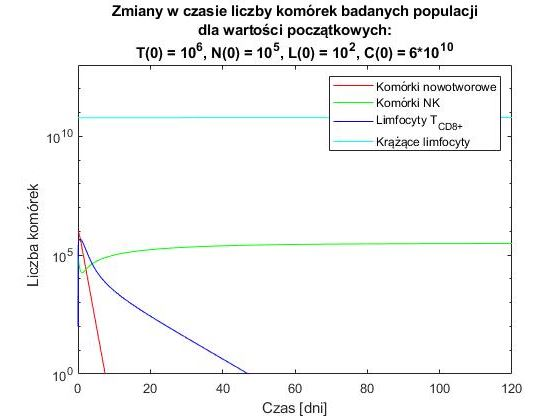
\includegraphics[width=0.85\textwidth]{bez_lecz_sym1_regresja}
\caption{Zmiany w~czasie liczby kom�rek badanych populacji dla~warto�ci pocz�tkowej liczby kom�rek nowotworowych $T(0) = 1 \cdot 10^{6}$. Widoczna (linia czerwona) regresja nowotworu po~czasie $T_{r}$~$\approx$ 7 dni (168 godzin).}
\label{bez_lecz_stlumienie}
\end{figure}

%\setlength{\parindent}{0pt}

\newpage
W drugiej cz�ci pracy przeprowadzono modelowanie odpowiedzi uk�adu immunologicznego na~rozwijaj�cy si� nowotw�r z~uwzgl�dnieniem leczenia:
\begin{itemize}
\item wy��cznie metod� chemioterapii,
\item wy��cznie metod� immunoterapii,
\item skojarzonymi metodami chemioterapii i~immunoterapii.
\end{itemize}

Jako warunki pocz�tkowe przyj�to takie warto�ci pocz�tkowej liczby kom�rek nowotworowych $T(0) = 1,8 \cdot 10^{7}$ i~limfocyt�w kr���cych $C(0) = 3,5 \cdot 10^{9}$, dla~kt�rych uk�ad immunologiczny nie~jest w~stanie (jak wynika z~symulacji opisanych w~rozdzia�ach \ref{bez_s1} i~\ref{bez_s2}) pokona� nowotworu bez zastosowania leczenia. Warunki pocz�tkowe (Tab. \ref{warunki_poczatkowe_z1}) reprezentuj� os�abiony uk�ad immunologiczny. \newline

\begin{table}[!htb]
	\centering
	\caption{Warunki pocz�tkowe dla~modelu odpowiedzi immunologicznej na~rozwijaj�cy si� nowotw�r z~uwzgl�dnieniem procesu leczenia.}\label{warunki_poczatkowe_z1}
	\begin{tabular}{|c|c|c|} \hline
		Pocz�tkowa & Rodzaj & Pocz�tkowa d�ugo��\\
		liczba kom�rek & kom�rek & promienia nowotworu $R_{0}$ [$mm$]\\ \hline
		$T(0) = 1,8 \cdot 10^{7}$ & Kom�rki nowotworowe & 1,63 \\ \hline
		$N(0) = 1 \cdot 10^{5}$ & Kom�rki NK \\ \cline{1-2}
		$L(0) = 1 \cdot 10^{2}$ & Limfocyty $T_{CD8+}$ \\ \cline{1-2}
		$C(0) = 3,5 \cdot 10^{9}$ & Limfocyty kr���ce \\ \cline{1-2}
		\end{tabular}
\end{table}

Warto�ci parametr�w (Tab. \ref{parametry_modelu_bez1}) oraz~warto�ci dodatkowych parametr�w uwzgl�dniaj�cych proces leczenia (Tab. \ref{parametry_modelu_z1}) dla~modelu \ref{r�wnania_modelu_pillis_z_leczeniem} dobrano zgodnie z~literatur� \cite{19}.

\begin{table}[h!]
	\centering
	\caption{Warto�ci dodatkowych parametr�w modelu odpowiedzi immunologicznej na~rozwijaj�cy si� nowotw�r z~uwzgl�dnieniem procesu leczenia.}\label{parametry_modelu_z1}
	\begin{tabular}{|c|c|c|c|c|c|c|c|c|} \hline
		Nazwa & $\gamma$ & $K_{T}$ & $K_{N}$ & $K_{L}$ & $K_{C}$ & $p_{I}$ & $g_{I}$ & $\mu_{I}$ \\ \hline
		Warto�� & $9 \cdot 10^{-1}$ & $9 \cdot 10^{-1}$ & $6 \cdot 10^{-1}$ & $6 \cdot 10^{-1}$ & $6 \cdot 10^{-1}$ & $9 \cdot 10^{3}$ & $2 \cdot 10^{7}$ & $1 \cdot 10^{1}$ \\ \hline	
	\end{tabular}
\end{table}

Rys. \ref{diagram_analiz} przedstawia analizy, jakie wykonano oraz~opisano w~niniejszej pracy, zar�wno dla~braku leczenia, jak~i~leczenia metodami chemioterapii, immunoterapii oraz~skojarzonymi metodami chemioterapii i~immunoterapii.

\begin{figure}[!h]
	\centering
	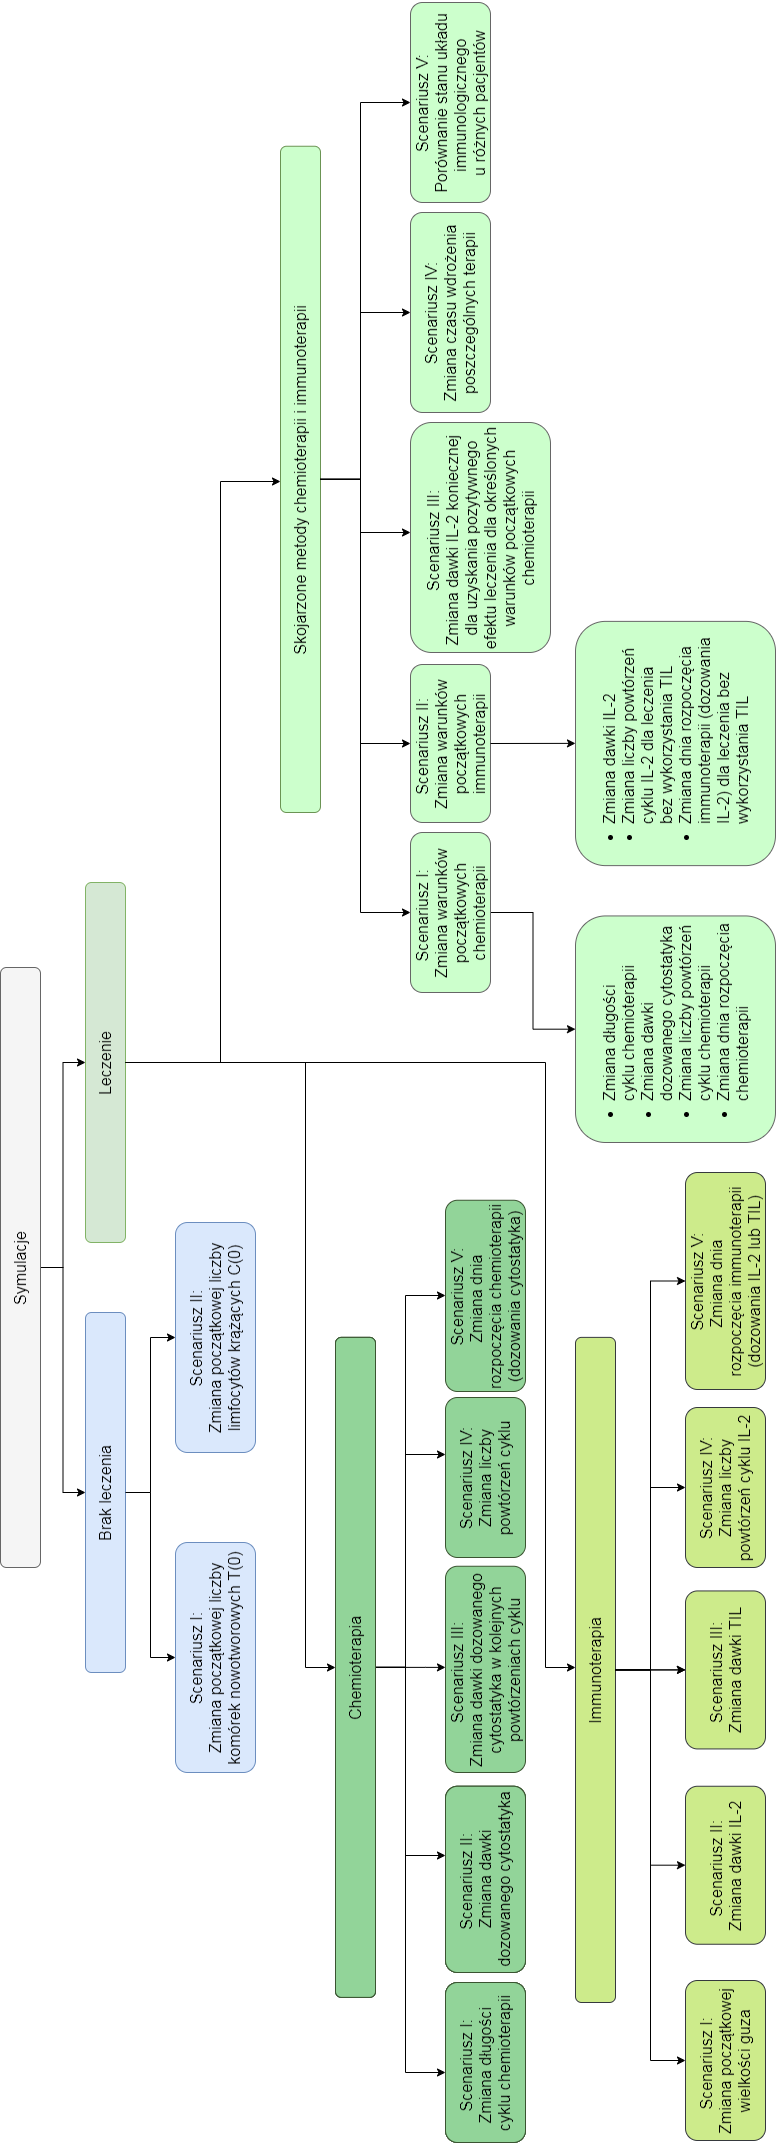
\includegraphics[width=0.55\textwidth]{diagram_analiz}
	\caption{Schemat przeprowadzonych w~niniejszej pracy analiz rozwoju guza, bez i~z~uwzgl�dnieniem terapii.}\label{diagram_analiz} 
\end{figure}

\chapter{Symulacje modelu rozwoju nieleczonego guza}

\section{Scenariusz I -- zmiana pocz�tkowej liczby kom�rek nowotworowych} \label{bez_s1}

\noindent \textbf{Podejmowany problem:} \newline Analiza zmian odpowiedzi uk�adu immunologicznego (tj. liczby kom�rek nowotworowych oraz~kom�rek uk�adu odporno�ciowego) w~ostatnim dniu symulacji w~zale�no�ci od~pocz�tkowej liczby kom�rek nowotworowych.

\noindent \newline \textbf{Warunki pocz�tkowe:} \newline Wielko�� (tj. pocz�tkow� liczb� kom�rek) nowotworu $T(0)$, liczb� kom�rek NK $N(0)$, liczb� limfocyt�w $T_{CD8+}$ oraz~liczb� limfocyt�w kr���cych $C(0)$ przedstawia~Tab. \ref{warunki_poczatkowe_bez1}.

\noindent \newline \textbf{Przyj�te parametry:} \newline Parametry dla~modelu nieuwzgl�dniaj�cego leczenia przedstawia~Tab. \ref{parametry_modelu_bez1}.

\noindent \newline \textbf{Czas symulacji:} \newline Czas symulacji wynosi� $T_{k}$ = 120 dni. 

\noindent \newline \textbf{Wyniki symulacji:} \newline Wyniki przeprowadzonych symulacji dla~zmieniaj�cej si� pocz�tkowej liczby kom�rek nowotworowych $T(0)$ zebrano w~Tab. \ref{zmiany_poczatkowej_wartosci_T_brak_leczenia}. \newline

\newpage
Tab. \ref{zmiany_poczatkowej_wartosci_T_brak_leczenia} przedstawia zale�no�� liczby kom�rek nowotworu w~ostatnim dniu symulacji, tj. w~chwili $T_{k}$ = 120 dni $T(120)$ od zmieniaj�cej si� pocz�tkowej liczby kom�rek nowotworu $T(0)$. Dodatkowo, w~tabeli zamieszczono szacowan� obj�to�� i~d�ugo�� promienia nowotworu w~ostatnim dniu symulacji.

\begin{table}[h!]
\small
	\centering
	\caption[Wyniki symulacji - brak leczenia, scenariusz I]{Pocz�tkowa liczba kom�rek nowotworowych $T(0)$, pocz�tkowa szacowana d�ugo�� promienia nowotworu $R_{0}$, liczba kom�rek nowotworowych w~ostatnim dniu symulacji w~chwili $T_{k}$ = 120 dni $T(120)$ oraz~szacowana obj�to�� i~d�ugo�� promienia nowotworu po~120~dniach symulacji w~chwili $T_{k}$ = 120 dni.}
\label{zmiany_poczatkowej_wartosci_T_brak_leczenia}
\begin{tabular}{|c|c|c|c|c|c|} \hline
		$T(0)$ & Pocz�tkowa d�ugo�� & $T(120)$ & Obj�to�� & D�ugo�� promienia \\
		$[liczba$ & promienia nowotworu & $[liczba$ & nowotworu & nowotworu \\
		$kom$�$rek]$ & $R_{0}$ [$mm$] & $kom$�$rek]$ & [$mm^{3}$] & [$mm$] \\ \hline
		$1 \cdot 10^{6}$ & 0,62 & $6,76 \cdot 10^{-8}$ & $6,76 \cdot 10^{-14}$ & $2,5 \cdot 10^{-5}$ \\ \hline
		$2 \cdot 10^{6}$ & 0,78 & $8,15 \cdot 10^{-8}$ & $8,15 \cdot 10^{-14}$ & $2,7 \cdot 10^{-5}$ \\ \hline
		$5 \cdot 10^{6}$ & 1,06 & $2,69 \cdot 10^{-8}$ & $2,69 \cdot 10^{-14}$ & $1,9 \cdot 10^{-5}$ \\ \hline
		$1 \cdot 10^{7}$ & 1,34 & $3,44 \cdot 10^{-8}$ & $3,44 \cdot 10^{-14}$ & $2 \cdot 10^{-5}$ \\ \hline
		$1,5 \cdot 10^{7}$ & 1,53 & $4,41 \cdot 10^{-8}$ & $4,41 \cdot 10^{-14}$ & $2,2 \cdot 10^{-5}$ \\ \hline
		$1,7 \cdot 10^{7}$ & 1,6 & $2,96 \cdot 10^{-8}$ & $2,96 \cdot 10^{-14}$ & $1,9 \cdot 10^{-5}$ \\ \hline
		$1,75 \cdot 10^{7}$ & 1,61 & $3,67 \cdot 10^{-8}$ & $3,67 \cdot 10^{-14}$ & $2,1 \cdot 10^{-5}$ \\ \hline
		$1,8 \cdot 10^{7}$ & 1,63 & $9,8 \cdot 10^{8}$ & $980$ & $6,16$ \\ \hline
		$2 \cdot 10^{7}$ & 1,69 & $9,8 \cdot 10^{8}$ & $980$ & $6,16$ \\ \hline
		$5 \cdot 10^{7}$ & 2,29 & $9,8 \cdot 10^{8}$ & $980$ & $6,16$ \\ \hline
		\end{tabular}
\end{table} 

\normalsize
\newpage
Zmiany wielko�ci nowotworu obserwowane w~ostatnim dniu symulacji $T_{k}$ = 120~dni w~zale�no�ci od~pocz�tkowej liczby kom�rek nowotworowych $T(0)$ przedstawia Rys.~\ref{wykres_bez_lecz_t120_t0_zmiana_T}. Z kolei Rys. \ref{wykres_bez_lecz_promien_t0_zmiana_T} przedstawia zmiany d�ugo�ci promienia nowotworu obserwowane w~ostatnim (120) dniu symulacji w~zale�no�ci od~pocz�tkowej liczby kom�rek nowotworowych $T(0)$.

\begin{figure}[h!]
\centering
\subfloat[Zale�no�� liczby kom�rek nowotworowych w~ostatnim 120 dniu symulacji ($T_{k}$ = 120 dni) od~pocz�tkowej liczby kom�rek nowotworowych $T(0)$.]{\label{wykres_bez_lecz_t120_t0_zmiana_T}
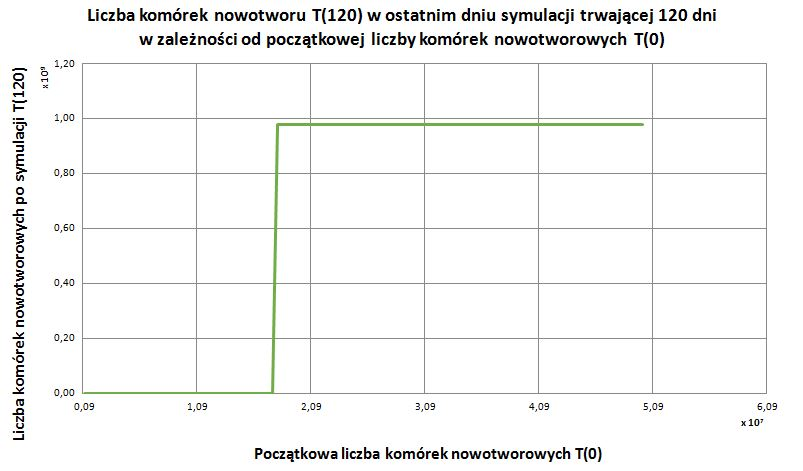
\includegraphics[width=0.75\textwidth]{wykres_bez_lecz_t120_t0}}
\quad
\subfloat[Zale�no�� d�ugo�ci promienia nowotworu w~ostatnim 120~dniu symulacji ($T_{k}$ = 120 dni) od~pocz�tkowej liczby kom�rek nowotworowych $T(0)$.]{\label{wykres_bez_lecz_promien_t0_zmiana_T}
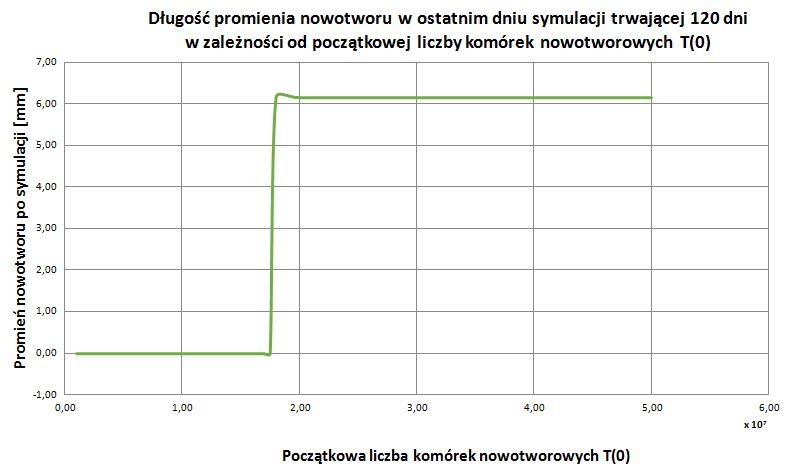
\includegraphics[width=0.75\textwidth]{wykres_bez_lecz_promien_t0}}
\caption{Wyniki obserwowane w~ostatnim dniu symulacji $T_{k}$ = 120 dni. Liczba kom�rek nowotworowych oraz~d�ugo�� promienia nowotworu [mm] w~ostatnim (120) dniu symulacji w~zale�no�ci od~pocz�tkowej liczby kom�rek nowotworowych $T(0)$.}
\label{zmiany_t120_i_promien_w_zaleznosci_od_t0}
\end{figure}

\newpage
Przyk�adowo, Rys. \ref{bez_lecz_brak_stlumienia_zmiana_T} przedstawia przypadek, w~kt�rym uk�ad immunologiczny nie~jest w~stanie zwalczy� nowotworu -- liczba jego kom�rek stabilizuje si� po~oko�o 24~dniach oko�o warto�ci $9,8 \cdot 10^{8}$ (co~odpowiada obj�to�ci 980 $mm^{3}$ i~d�ugo�ci promienia 6,16 $mm$).

\begin{figure}[h!]
\centering
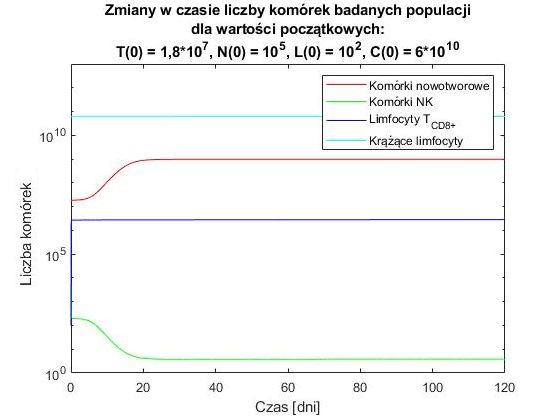
\includegraphics[width=0.65\textwidth]{bez_lecz_sym1_progres}
\caption[Zmiany w~czasie liczby kom�rek badanych populacji - brak leczenia, scenariusz I]{Zmiany w~czasie liczby kom�rek badanych populacji dla~warto�ci pocz�tkowej liczby kom�rek nowotworowych $T(0) = 1.8 \cdot 10^{7}$. Po~czasie $T_{s}$~$\approx$ 24 dni (576 godzin) widoczna (linia czerwona) stabilizacja liczby kom�rek nowotworowych oko�o warto�ci $9,8 \cdot 10^{8}$.}
\label{bez_lecz_brak_stlumienia_zmiana_T}
\end{figure}

\textbf{Wnioski:}
\begin{itemize}
\item zdrowy uk�ad immunologiczny, reprezentowany przez liczb� kom�rek wyst�puj�cych naturalnie w~organizmie: kom�rek NK $N(0) = 10^{5}$, limfocyt�w $T_{CD8+}$ $L(0) = 10^{2}$ oraz~limfocyt�w kr���cych $C(0) = 6 \cdot 10^{10}$ jest w~stanie zniszczy� (Rys. \ref{bez_lecz_stlumienie}) kom�rki nowotworowe bez ingerencji dodatkowych czynnik�w (np. leczenia), je�li pocz�tkowa liczba kom�rek nowotworu wynosi $T(0) = 10^{6}$ kom�rek (wielko��, przy kt�rej guz jest wykrywalny klinicznie);
\item przy~zbyt~du�ej pocz�tkowej liczbie kom�rek nowotworu ($T(0) \approx 1,8 \cdot 10^{7}$) uk�ad immunologiczny, mimo dobrej kondycji, nie~potrafi samoistnie zwalczy� nowotworu (Rys. \ref{bez_lecz_brak_stlumienia_zmiana_T});
\item wzrost liczby kom�rek nowotworowych powoduje nag�y przyrost limfocyt�w $T_{CD8+}$ wywo�any nieudan� pr�b� zniszczenia nowotworu; liczba limfocyt�w $T_{CD8+}$ utrzymuje si� (nie zmniejsza si�) na~poziomie $L \approx 2,8 \cdot 10^{6}$ kom�rek;
\item na~skutek interakcji, tj. pr�by zniszczenia kom�rek nowotworu przez~kom�rki NK, liczba kom�rek NK maleje i~utrzymuje si� na~zbyt niskim poziomie $N \approx 3,78$ kom�rek;
\item liczba limfocyt�w kr���cych, mimo zmian w~czasie pozosta�ych populacji, utrzymuje si� na~poziomie $C \approx 6 \cdot 10^{10}$ kom�rek;
\end{itemize}

Analiza zmian pocz�tkowej wielko�ci guza wykaza�a, �e istnieje mo�liwo�� samoistnego pokonania nowotworu przez~organizm pacjenta, o~ile pocz�tkowa liczba kom�rek nowotworu T(0) nie~przekroczy pewnej warto�ci. Je�li pocz�tkowa liczba kom�rek nowotworowych pacjenta przekracza $T(0) = 1,8 \cdot 10^{7}$, konieczne jest wdro�enie leczenia.

\newpage
\section{Scenariusz II -- zmiana pocz�tkowej liczby limfocyt�w kr���cych} \label{bez_s2}

\noindent \textbf{Podejmowany problem:} \newline Analiza zmian odpowiedzi uk�adu immunologicznego (tj. liczby kom�rek nowotworowych oraz~kom�rek uk�adu odporno�ciowego) w~ostatnim dniu symulacji w~zale�no�ci od~pocz�tkowej liczby limfocyt�w kr���cych $C(0)$.

\noindent \newline \textbf{Warunki pocz�tkowe:} \newline Wielko�� (tj. pocz�tkow� liczb� kom�rek) nowotworu $T(0)$, liczb� kom�rek NK $N(0)$, liczb� limfocyt�w $T_{CD8+}$ oraz~liczb� limfocyt�w kr���cych $C(0)$ przedstawia~Tab. \ref{warunki_poczatkowe_bez1}.

\noindent \newline \textbf{Przyj�te parametry:} \newline Parametry dla~modelu nieuwzgl�dniaj�cego leczenia przedstawia~Tab. \ref{parametry_modelu_bez1}.

\noindent \newline \textbf{Czas symulacji:} \newline Czas symulacji wynosi� $T_{k}$ = 120 dni.

\noindent \newline \textbf{Wyniki symulacji:} \newline Wyniki przeprowadzonych symulacji dla~zmieniaj�cej si� pocz�tkowej liczby limfocyt�w kr���cych $C(0)$ zebrano w~Tab. \ref{zmiany_poczatkowej_wartosci_C}. \newline

Tab. \ref{zmiany_poczatkowej_wartosci_C} przedstawia zale�no�� liczby kom�rek nowotworu w~ostatnim (120) dniu symulacji od~zmieniaj�cej~si� pocz�tkowej liczby limfocyt�w kr���cych $C(0)$. Dodatkowo, w~tabeli zamieszczono szacowan� obj�to�� i~d�ugo�� promienia nowotworu w~ostatnim dniu symulacji, tj. w~chwili $T_{k}$ = 120 dni.

\begin{table}[!htb]
	\centering
	\caption[Wyniki symulacji - brak leczenia, scenariusz II]{Pocz�tkowa liczba limfocyt�w kr���cych $C(0)$, liczba kom�rek nowotworowych w~ostatnim (120) dniu symulacji oraz~szacowana obj�to�� i~d�ugo�� promienia nowotworu w~ostatnim dniu symulacji w~chwili $T_{k}$ = 120 dni.}\label{zmiany_poczatkowej_wartosci_C}
\begin{tabular}{|c|c|c|c|} \hline
		$C(0)$ & $T(120)$ & Obj�to�� & D�ugo�� promienia \\
		$[liczba$ $kom$�$rek]$ & $[liczba$ $kom$�$rek]$ & nowotworu [$mm^{3}$] & nowotworu [$mm$] \\ \hline
		$6 \cdot 10^{10}$ & $6,76 \cdot 10^{-8}$ & $6,76 \cdot 10^{-14}$ & $2,5 \cdot 10^{-5}$ \\ \hline
		$3 \cdot 10^{10}$ & $1,69 \cdot 10^{-7}$ & $1,69 \cdot 10^{-13}$ & $3,4 \cdot 10^{-5}$ \\ \hline
		$1 \cdot 10^{10}$ & $3,09 \cdot 10^{-8}$ & $1,33 \cdot 10^{-14}$ & $1,5 \cdot 10^{-5}$ \\ \hline
		$6 \cdot 10^{9}$ & $4,79 \cdot 10^{-8}$ & $4,79 \cdot 10^{-14}$ & $2,3 \cdot 10^{-5}$ \\ \hline
		$4 \cdot 10^{9}$ & $5,72 \cdot 10^{-8}$ & $5,72 \cdot 10^{-14}$ & $2,4 \cdot 10^{-5}$ \\ \hline
		$3,5 \cdot 10^{9}$ & $9,8 \cdot 10^{8}$ & $980$ & $6,16$ \\ \hline
		$3 \cdot 10^{9}$ & $9,8 \cdot 10^{8}$ & $980$ & $6,16$ \\ \hline
		$1 \cdot 10^{9}$ & $9,8 \cdot 10^{8}$ & $980$ & $6,16$ \\ \hline
		$6 \cdot 10^{8}$ & $9,8 \cdot 10^{8}$ & $980$ & $6,16$ \\ \hline
		$3 \cdot 10^{8}$ & $9,8 \cdot 10^{8}$ & $980$ & $6,16$ \\ \hline
		\end{tabular}
\end{table}

Zmiany w~czasie wielko�ci nowotworu obserwowane po 120 dniach symulacji ($T_{k}$ = 120 dni) w~zale�no�ci od~pocz�tkowej liczby kr���cych limfocyt�w $C(0)$ przedstawia Rys. \ref{wykres_bez_lecz_t120_c0}. Rys. \ref{wykres_bez_lecz_promien_c0} przedstawia zmiany d�ugo�ci promienia nowotworu obserwowane w~ostatnim (120) dniu symulacji w~zale�no�ci od~pocz�tkowej liczby kr���cych limfocyt�w $C(0)$.

\begin{figure}[h!]
\centering
\subfloat[Zale�no�� liczby kom�rek nowotworowych w ostatnim (120) dniu symulacji ($T_{k}$ = 120 dni) od~pocz�tkowej liczby kr���cych limfocyt�w $C(0)$.]{\label{wykres_bez_lecz_t120_c0}
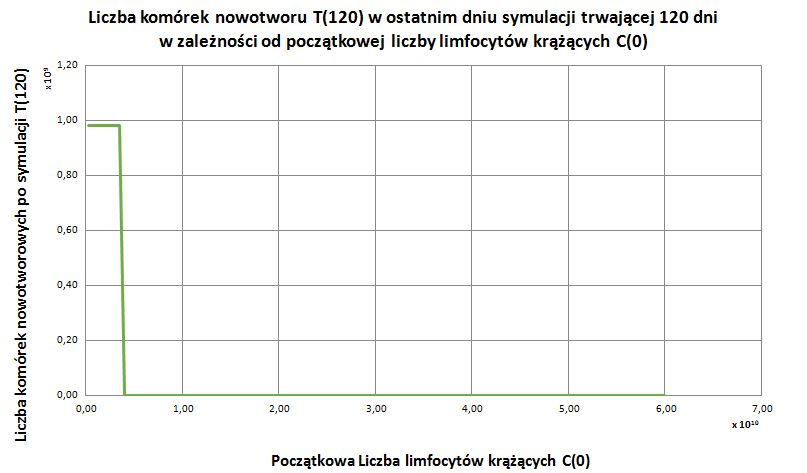
\includegraphics[width=0.75\textwidth]{wykres_bez_lecz_t120_c0}}
\quad
\subfloat[Zale�no�� d�ugo�ci promienia nowotworu w ostatnim (120) dniu symulacji ($T_{k}$ = 120 dni) od~pocz�tkowej liczby kr���cych limfocyt�w $C(0)$.]{\label{wykres_bez_lecz_promien_c0}
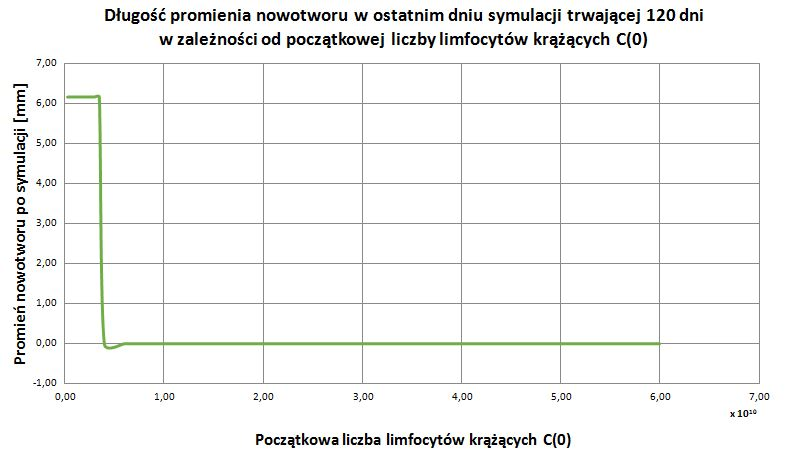
\includegraphics[width=0.75\textwidth]{wykres_bez_lecz_promien_c0}}
\caption{Wyniki obserwowane w~ostatnim dniu symulacji $T_{k}$ = 120 dni. Liczba kom�rek nowotworowych oraz~d�ugo�� promienia nowotworu [mm] w~ostatnim (120) dniu symulacji w~zale�no�ci od~pocz�tkowej liczby kr���cych limfocyt�w $C(0)$.}
\label{zmiany_t120_i_promien_w_zaleznosci_od_c0}
\end{figure}

\newpage
Przyk�adowo, Rys. \ref{zmiany_liczby_kom_4_populacjiC} przedstawia sytuacj�, w~kt�rej uk�ad immunologiczny ze~wzgl�du na~zmniejszon� liczb� kr���cych limfocyt�w jest zbyt s�aby, by~zniszczy� kom�rki nowotworu. Liczba kom�rek nowotworowych ro�nie i~po~oko�o 28 dniach stabilizuje si� oko�o warto�ci $9,8 \cdot 10^{8}$. 

\begin{figure}[h!]
\centering
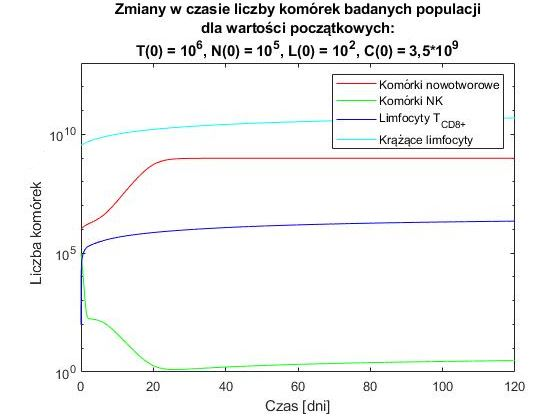
\includegraphics[width=0.75\textwidth]{bez_lecz_sym2_progres}
\caption[Zmiany w~czasie liczby kom�rek badanych populacji - brak leczenia, scenariusz II]{Zmiany liczby kom�rek badanych populacji dla~warto�ci pocz�tkowej liczby limfocyt�w kr���cych C(0) = $3, 5 \cdot 10^{9}$. Po~czasie $T_{s} \approx 28$ dni (672 godziny) widoczna (linia czerwona) stabilizacja liczby kom�rek nowotworowych oko�o warto�ci $9, 8 \cdot 10^{8}$.}
\label{zmiany_liczby_kom_4_populacjiC}
\end{figure}

\textbf{Wnioski:}
\begin{itemize}
\item przy~du�ej pocz�tkowej liczbie ($C(0) \approx 4 \cdot 10^{9}$) kr���cych limfocyt�w, uk�ad immunologiczny jest w~stanie zniszczy� kom�rki nowotworowe bez ingerencji zewn�trznych czynnik�w (np. leczenia);
\item przy~obni�onej liczbie kr���cych limfocyt�w (oznaczaj�cej s�ab� kondycj� uk�adu immunologicznego) organizm nie~jest w~stanie zniszczy� kom�rek nowotworu;
\item w~symulacji opisanej w rozdziale \ref{bez_s1} liczba kr���cych limfocyt�w pozostawa�a na~sta�ym poziomie, mo�na wi�c wnioskowa�, �e zmiany liczby kom�rek nowotworowych i~limfocyt�w $T_{CD8}$ s�~niezale�ne od~liczby limfocyt�w kr���cych, jednak w~symulacji \ref{bez_s2} wida�, �e stosunkowo niewielka zmiana liczby limfocyt�w kr���cych znacz�co wp�ywa na~wynik symulacji;
\end{itemize} 

Dzi�ki analizie zmian pocz�tkowej liczby limfocyt�w kr���cych C(0) mo�na wnioskowa�, �e mimo stosunkowo niewielkiego zmniejszenia liczby tych limfocyt�w, maj�~one znaczny wp�yw na~odpowied� immunologiczn� organizmu. Mimo liczby limfocyt�w kr���cych o~warto�ci rz�du $10^{9}$, organizm jest zbyt os�abiony, by~zwalczy� nowotw�r.

\chapter{Leczenie metod� chemioterapii -- symulacje wykonane dla~modelu leczonego guza} \label{sym_ch}

W symulacji leczenia metod� chemioterapii wzi�to pod uwag� takie zmienne, jak:
\begin{itemize}
\item d�ugo�� cyklu dozowania cytostatyka (okre�laj�ca czas przerw pomi�dzy kolejnymi dozowanymi dawkami),
\item czas dozowania cytostatyka podczas jednego cyklu,
\item dawka dozowanego cytostatyka $V_M$,
\item liczba powt�rze� cyklu dozowania cytostatyka,
\item dzie� rozpocz�cia leczenia.
\end{itemize} 

Cykl podawania leku okre�la czas ci�g�ego podawania leku oraz~przerwy pomi�dzy kolejnymi dawkami konieczne do~regeneracji organizmu. Przyk�adowy schemat cyklu [1 5] oznacza podawanie leku przez~1-dzie� (24 godziny) oraz~5-dni (120 godzin) przerwy. Podczas terapii cykl mo�e zosta� powt�rzony, co~oznacza kolejny 1 dzie� podawania leku, i~kolejne 5 dni przerwy.

\begin{table}[h!]
\small
	\centering
	\caption{Warunki pocz�tkowe modelu odpowiedzi immunologicznej na~rozwijaj�cy si� nowotw�r z~uwzgl�dnieniem procesu leczenia za~pomoc� chemioterapii.}\label{warunki pocz�tkowe_chemioterapii}
\begin{tabular}{|c|c|c|c|c|c|} \hline
		D�ugo�� & Czas dozowania & Schemat & Dawka & Liczba & Dzie� \\
		cyklu & cytostatyka & cyklu & dozowanego & powt�rze� & rozpocz�cia \\
		$[dni]$ & $[dni]$ & [dozowanie & cytostatyka & cyklu & chemioterapii \\
		 & & przerwa] & $V_M$ $[\dfrac{mg}{m^{2}}]$ &  &  \\ \hline 
		4 & 1 & [1 3] & 5 & 9 & 1 \\ \hline
		\end{tabular}
\end{table} 

We~wszystkich symulacjach leczenia metod� chemioterapii analizowano zmiany odpowiedzi uk�adu immunologicznego (tj. liczby kom�rek nowotworowych oraz~kom�rek uk�adu odporno�ciowego) po~120 dniach ($T_{k} = 120$ dni) symulacji w~zale�no�ci od~wy�ej wymienionych zmiennych okre�laj�cych chemioterapi�.

\newpage
\section{Scenariusz I -- zmiana d�ugo�ci cyklu}\label{chemio_zmiana_dlugosci_cyklu}

\noindent \textbf{Podejmowany problem:} \newline Wp�yw zmian d�ugo�ci cyklu chemioterapii, tj. czasu dozowania cytostatyka oraz~przerw pomi�dzy kolejnymi dozowanymi dawkami na~skuteczno�� terapii.

\noindent \newline \textbf{Warunki pocz�tkowe:} 
\begin{itemize}
\item dla~pocz�tkowej wielko�ci badanych populacji, tj. pocz�tkow� liczb� kom�rek nowotworu $T(0)$, liczb� kom�rek NK $N(0)$, liczb� limfocyt�w $T_{CD8+}$ oraz~liczb� limfocyt�w kr���cych $C(0)$ przedstawia Tab. \ref{warunki_poczatkowe_z1};
\item dla~chemioterapii, tj. d�ugo�� cyklu, czas dozowania cytostatyka, schemat cyklu, dawk� dozowanego cytostatyka $V_M$, liczb� powt�rze� cyklu oraz~dzie� rozpocz�cia chemioterapii przedstawia Tab.~\ref{warunki pocz�tkowe_chemioterapii}. 
\end{itemize}

\noindent \newline \textbf{Przyj�te parametry:} \newline Parametry dla~modelu uwzgl�dniaj�cego leczenie przedstawia Tab. \ref{parametry_modelu_bez1} i~\ref{parametry_modelu_z1}.

\noindent \newline \textbf{Czas symulacji:} \newline Czas symulacji wynosi� $T_{k}$ = 120 dni. 

\noindent \newline \textbf{Wyniki symulacji:} \newline Wyniki przeprowadzonych symulacji dla~zmian d�ugo�ci cyklu zebrano w~Tab.~\ref{chemio_zmiany_liczby_dni_cyklu}. \newline

Tab. \ref{chemio_zmiany_liczby_dni_cyklu} przedstawia zmiany d�ugo�ci cyklu (d�ugo�� przerw pomi�dzy dawkami przy sta�ym czasie dozowania cytostatyka oraz~czas dozowania cytostatyka przy sta�ej d�ugo�ci przerw pomi�dzy dawkami) chemioterapii oraz~schemat cyklu. Dodatkowo, w~Tab. \ref{chemio_zmiany_liczby_dni_cyklu} umieszczono dzie� regresji nowotworu oraz~liczb� kom�rek nowotworu T(120) w~ostatnim (120) dniu symulacji, a~tak�e, dla~�atwiejszego zobrazowania otrzymanych wynik�w, szacowan� obj�to�� i~d�ugo�� promienia nowotworu w~ostatnim (120) dniu symulacji (tj. w~chwili $T_{k}$ = 120 dni).

\begin{table}[h!]
	\centering
	\caption[Wyniki symulacji - chemioterapia, scenariusz I, zmiana d�ugo�ci cyklu]{D�ugo�� oraz~schemat cyklu chemioterapii, dzie� regresji nowotworu, liczba kom�rek nowotworowych T(120) w~ostatnim (120) dniu symulacji oraz~szacowana obj�to�� i~d�ugo�� promienia nowotworu w~ostatnim (120) dniu symulacji (tj. w~chwili $T_{k}$ = 120 dni) dla~zmieniaj�cej si� d�ugo�ci przerw pomi�dzy poszczeg�lnymi dawkami chemioterapii (przy sta�ym czasie dozowania pojedynczej dawki r�wnym 1 dzie� (24 godziny)) oraz~zmieniaj�cego si� czasu dozowania pojedynczej dawki (przy sta�ej d�ugo�ci przerwy pomi�dzy dawkami r�wnej 3 dni (72 godziny)).}\label{chemio_zmiany_liczby_dni_cyklu}
\begin{tabular}{|c|c|c|c|c|c|} \hline \hline
        \multicolumn{6}{|c|}{Zmiana d�ugo�ci \textbf{przerwy} pomi�dzy dawkami} \\ \hline \hline
		D�ugo�� & Schemat & Dzie� & $T(120)$ & Obj�to�� & D�ugo�� promienia \\
		cyklu & cyklu & regresji & $[liczba$ & nowotworu & nowotworu [$mm$] \\
		$[dni]$ & & nowotworu & $kom$�$rek]$ & [$mm^{3}$] & \\ \hline
		4 & [1 \textbf{3}] & 25,84 & $4,64 \cdot 10^{-8}$ & $4,64 \cdot 10^{-14}$ & $2,2 \cdot 10^{-5}$ \\ \hline
		4,5 & [1 \textbf{3,5}] & 32,25 & $2,46 \cdot 10^{-7}$ & $2,46 \cdot 10^{-13}$ & $3,9 \cdot 10^{-5}$ \\ \hline
		5 & [1 \textbf{4}] & 45,1 & $9,37 \cdot 10^{-8}$ & $9,37 \cdot 10^{-14}$ & $2,8 \cdot 10^{-5}$ \\ \hline
		5,5 & [1 \textbf{4,5}] & brak & $9,8 \cdot 10^{8}$ & $980$ & $6,16$ \\ \hline
		8 & [1 \textbf{7}] & brak & $9,8 \cdot 10^{8}$ & $980$ & $6,16$ \\ \hline
		12 & [1 \textbf{11}] & brak & $9,8 \cdot 10^{8}$ & $980$ & $6,16$ \\ \hline \hline
		 \multicolumn{6}{|c|}{Zmiana \textbf{czasu dozowania} poszczeg�lnych dawek} \\ \hline \hline
		D�ugo�� & Schemat & Dzie� & $T(120)$ & Obj�to�� & D�ugo�� promienia \\
		cyklu & cyklu & regresji & $[liczba$ & nowotworu & nowotworu [$mm$] \\
		$[dni]$ & & nowotworu & $kom$�$rek]$ & [$mm^{3}$] & \\ \hline
		4 & [\textbf{1} 3] & 25,84 & $4,64 \cdot 10^{-8}$ & $4,64 \cdot 10^{-14}$ & $2,2 \cdot 10^{-5}$ \\ \hline
		3,75 & [\textbf{0,75} 3] & 34,34 & $8,94 \cdot 10^{-8}$ & $8,94 \cdot 10^{-14}$ & $2,8 \cdot 10^{-5}$ \\ \hline
		3,5 & [\textbf{0,5} 3] & brak & $9,8 \cdot 10^{8}$ & $980$ & $6,16$ \\ \hline
		\end{tabular}
\end{table}

\newpage
Przyk�adowo, Rys. \ref{wykresy_chemio_zmiany_liczby_dni_cyklu} przedstawia zmiany w~czasie liczby kom�rek badanych populacji, tj. kom�rek nowotworowych, kom�rek NK, limfocyt�w $T_{CD8+}$ oraz~limfocyt�w kr���cych dla~d�ugo�ci cyklu chemioterapii wynosz�cej 4 (Rys. \ref{wykres_chemio_zmiany_liczby_dni_cyklu}) oraz~8 (Rys. \ref{wykres_chemio_zmiany_liczby_dni_cyklu8}) dni, a~tak�e zmiany w~czasie st�enia, dozowanego podczas chemioterapii, cytostatyka (Rys. \ref{stezenie_chemio_zmiany_liczby_dni_cyklu} i~\ref{stezenie_chemio_zmiany_liczby_dni_cyklu8}). 

Symulacja zak�ada�a rozpocz�cie chemioterapii (podanie pierwszej dawki cytostatyka) w~pierwszym dniu symulacji oraz~dziewi�ciokrotne powt�rzenie cyklu. Ka�de z~tych powt�rze� mo�na zaobserwowa� w~postaci pik�w na~wykresach zmian st�enia oraz~jako charakterystyczne za�amanie krzywych odpowiadaj�cych badanym populacjom (Rys. \ref{wykresy_chemio_zmiany_liczby_dni_cyklu}). We wszystkich powt�rzeniach dawka cytostatyka $V_M = 5$ $\dfrac{mg}{m^{2}}$, za�~czas podawania cytostatyka wynosi� 1 dzie� (24 godziny). D�ugo�� przerwy pomi�dzy kolejnymi powt�rzeniami by�a zale�na od~d�ugo�ci i~schematu cyklu. Dla 4-dniowego cyklu (schemat [1 3]) by�y~to 3 dni przerwy, natomiast dla~8-dniowego cyklu (schemat [1 7]) 7 dni przerwy. 

Podczas ka�dej z~przerw liczba kom�rek nowotworowych zaczyna�a ponownie wzrasta�. W przypadku cyklu trwaj�cego 4 dni czas przerwy by� zbyt kr�tki aby~kom�rki nowotworu znacznie si� rozmno�y�y, dlatego mo�liwa by�a regresja nowotworu, kt�ra nast�pi�a w~26 dniu symulacji. W przypadku cyklu trwaj�cego 8 dni, czas przerwy pomi�dzy dawkami by� wystarczaj�co d�ugi do~niekontrolowanego rozrostu nowotworu. Liczba kom�rek nowotworowych wzrasta�a i~ustabilizowa�a si� na~wysokim poziomie ($9,8 \cdot 10^{8}$) w~91 dniu symulacji (Rys. \ref{wykres_chemio_zmiany_liczby_dni_cyklu8}).

\begin{figure}[h!]
\centering
\subfloat[Zmiany w~czasie liczby kom�rek badanych populacji dla~4-dniowego cyklu chemioterapii. Widoczna (linia czerwona) regresja nowotworu po~26 dniach.]{\label{wykres_chemio_zmiany_liczby_dni_cyklu}
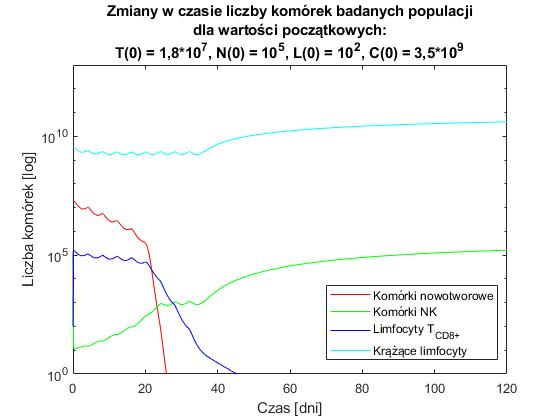
\includegraphics[width=0.45\textwidth]{wykres_chemio_zmiany_liczby_dni_cyklu}}
\quad
\subfloat[Zmiany w~czasie liczby kom�rek badanych populacji dla~8-dniowego cyklu chemioterapii. Widoczna (linia czerwona) stabilizacja liczby kom�rek nowotworowych w~91 dniu symulacji oko�o warto�ci $9,8 \cdot 10^{8}$.]{\label{wykres_chemio_zmiany_liczby_dni_cyklu8}
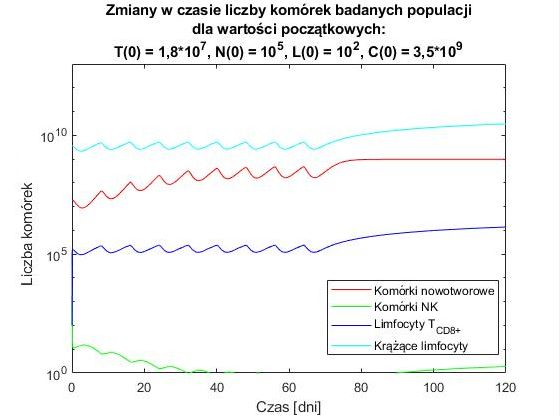
\includegraphics[width=0.45\textwidth]{wykres_chemio_zmiany_liczby_dni_cyklu8}}
\quad
\subfloat[Zmiany w~czasie st�enia, dozowanego podczas chemioterapii, cytostatyka dla~4-dniowego cyklu chemioterapii.]{\label{stezenie_chemio_zmiany_liczby_dni_cyklu}
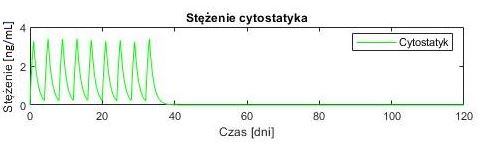
\includegraphics[width=0.45\textwidth]{stezenie_chemio_zmiany_liczby_dni_cyklu}}
\quad
\subfloat[Zmiany w~czasie st�enia, dozowanego podczas chemioterapii, cytostatyka dla~8-dniowego cyklu chemioterapii.]{\label{stezenie_chemio_zmiany_liczby_dni_cyklu8}
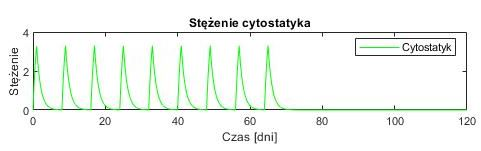
\includegraphics[width=0.45\textwidth]{stezenie_chemio_zmiany_liczby_dni_cyklu8}}
\caption[Zmiany w~czasie liczby kom�rek badanych populacji oraz~st�enia cytostatyka - chemioterapia, scenariusz I, zmiana d�ugo�ci cyklu]{Zmiany w~czasie liczby kom�rek badanych populacji oraz~st�enia dozowanego podczas chemioterapii cytostatyka dla~4-dniowego oraz~8-dniowego cyklu chemioterapii. Pocz�tkowa liczba kom�rek nowotworowych $T(0) = 1,8 \cdot 10^{7}$, pocz�tkowa liczba kom�rek NK $N(0) = 10^{5}$, pocz�tkowa liczba limfocyt�w $T_{CD8+}$ $L(0) = 10^{2}$, pocz�tkowa liczba limfocyt�w kr���cych $C(0) = 3,5 \cdot 10^{9}$.}
\label{wykresy_chemio_zmiany_liczby_dni_cyklu}
\end{figure}

\textbf{Wnioski:}
\begin{itemize}
\item os�abiony uk�ad immunologiczny, reprezentowany przez: kom�rki NK $N(0) = 10^{5}$, limfocyty $T_{CD8+}$ $L(0) = 10^{2}$ oraz~limfocyty kr���ce $C(0) = 3,5 \cdot 10^{9}$ wspomagany leczeniem metod� chemioterapii jest w~stanie zniszczy� kom�rki nowotworowe, je�li pocz�tkowa liczba kom�rek guza wynosi oko�o $T(0) = 1,8 \cdot 10^{7}$; 
\item d�ugo�� cyklu (tj. d�ugo�� przerwy pomi�dzy kolejnymi dawkami cytostatyka oraz~czas dozowania pojedynczej dawki cytostatyka) chemioterapii ma~wp�yw (im d�u�szy cykl, tym mniejsza skuteczno��) na~skuteczno�� tej metody leczenia (regresj� nowotworu lub jej brak) oraz~na~czas potrzebny do~regresji nowotworu;
\item regresja nowotworu nast�puje w~przypadku 4-dniowego cyklu chemioterapii, natomiast przy dwukrotnie oraz~trzykrotnie d�u�szym czasie cyklu nowotw�r nie~zostaje zniszczony;
\item dla~niewielkich zmian d�ugo�ci przerwy pomi�dzy podawaniem kolejnych dawek cytostatyka (d�ugo�� ta~wynosi�a: 3, 3,5 oraz~4 dni) czas konieczny do~regresji nowotworu znacznie si� wyd�u�y� (dzie�, w~kt�rym nast�pi�a regresja, odpowiednio: 26, 33 oraz~46); zatem wyd�u�enie przerwy mi�dzy dawkami o~p� dnia (12 godzin) skutkuje przed�u�eniem leczenia o~tydzie�, natomiast w~efekcie wyd�u�enia przerwy o~1 dzie� (24 godziny) terapia jest d�u�sza o~prawie 3 tygodnie (oko�o 2 razy d�u�ej ni�~w~przypadku, gdy przerwa wynosi 3 dni);
\item skr�cenie czasu podawania cytostatyka o~6 godzin przy sta�ej przerwie trwaj�cej 3 dni (72 godziny) powoduje przed�u�enie czasu koniecznego do~regresji nowotworu z~26 do~35 dni, natomiast skr�cenie tego czasu o~p� dnia (12 godzin) powoduje brak wyst�pienia regresji nowotworu.
\end{itemize}

Zmiany d�ugo�ci cyklu (zar�wno przerw pomi�dzy dawkami jak~i~czasu dawkowania) maj� znaczenie, je�li chodzi o~wywo�anie regresji nowotworu lub jej braku. Im cz�ciej powtarzane dozowanie, tym wi�ksza szansa na~zniszczenie kom�rek nowotworowych, jednak nale�y pami�ta� tak�e~o~szkodliwym wp�ywie cytostatyka na~zdrowe tkanki. Dzi�ki symulacjom mo�na oszacowa� d�ugo�� cyklu konieczn� do~osi�gni�cia pozytywnego efektu leczenia (tj. regresji nowotworu) przy~r�wnoczesnym ograniczeniu czasu dozowania cytostatyka.

\newpage
\section{Scenariusz II -- zmiana dawki dozowanego cytostatyka}
\noindent \textbf{Podejmowany problem:} \newline Wp�yw zmian dawki dozowanego cytostatyka $V_M$ na~skuteczno�� terapii. 

\noindent \newline \textbf{Warunki pocz�tkowe:} 
\begin{itemize}
\item dla~pocz�tkowej wielko�ci badanych populacji, tj. pocz�tkow� liczb� kom�rek nowotworu $T(0)$, liczb� kom�rek NK $N(0)$, liczb� limfocyt�w $T_{CD8+}$ oraz~liczb� limfocyt�w kr���cych $C(0)$ przedstawia Tab. \ref{warunki_poczatkowe_z1};
\item dla~chemioterapii, tj. czas dozowania cytostatyka, schemat cyklu, dawk� dozowanego cytostatyka $V_M$, liczb� powt�rze� cyklu oraz~dzie� rozpocz�cia chemioterapii przedstawia Tab.~\ref{warunki pocz�tkowe_chemioterapii}. D�ugo�� cyklu wynosi�a 4, 8 oraz~12 dni.
\end{itemize}

\noindent \newline \textbf{Przyj�te parametry:} \newline Parametry dla~modelu uwzgl�dniaj�cego leczenie przedstawia Tab. \ref{parametry_modelu_bez1} i~\ref{parametry_modelu_z1}.

\noindent \newline \textbf{Czas symulacji:} \newline Czas symulacji wynosi� $T_{k}$ = 120 dni. 

\noindent \newline \textbf{Wyniki symulacji:} \newline Wyniki przeprowadzonych symulacji dla~zmieniaj�cej si� dawki cytostatyka zebrano w~Tab. \ref{chemio_zmiany_dawki}. \newline

Tab. \ref{chemio_zmiany_dawki} przedstawia zmiany dawki dozowanego cytostatyka $V_M$ oraz~schemat cyklu chemioterapii. Dodatkowo, w~Tab. \ref{chemio_zmiany_dawki} zamieszczono dzie� regresji nowotworu oraz~liczb� kom�rek nowotworu T(120) w~ostatnim (120) dniu symulacji, a~tak�e~szacowan� obj�to�� i~d�ugo�� promienia nowotworu w~ostatnim (120) dniu symulacji (tj. w~chwili $T_{k}$ = 120 dni). Analiz� przeprowadzono dla~4-dniowego, 8-dniowego oraz~12-dniowego cyklu chemioterapii.

\begin{table}[h!]
\small
	\centering
	\caption[Wyniki symulacji - chemioterapia, scenariusz II, zmiana dawki dozowanego cytostatyka $V_M$]{Schemat cyklu chemioterapii, dawka dozowanego cytostatyka, dzie� regresji nowotworu, liczba kom�rek nowotworowych T(120) w~ostatnim (120) dniu symulacji oraz~szacowana obj�to�� i~d�ugo�� promienia nowotworu w~ostatnim (120) dniu symulacji (tj. w~chwili $T_{k}$ = 120 dni) dla~4-dniowego, 8-dniowego oraz~12-dniowego cyklu chemioterapii.}\label{chemio_zmiany_dawki}
\begin{tabular}{|c|c|c|c|c|c|} \hline \hline
        \multicolumn{6}{|c|}{\textbf{D�ugo�� cyklu: 4 dni}} \\ \hline \hline
		Schemat & Dawka & Dzie� & $T(120)$ & Obj�to�� & D�ugo�� promienia \\
	    cyklu & dozowanego & regresji & $[liczba$ & nowotworu & nowotworu\\ 
	    & cytostatyka & nowotworu & $kom$�$rek]$ & [$mm^{3}$] & [$mm$] \\
	    & $V_M$ $[\dfrac{mg}{m^{2}}]$ & & & & \\ \hline
		[1 3] & 3 & brak & $9,8 \cdot 10^{8}$ & $980$ & $6,16$ \\ \hline
		[1 3] & 3,5 & 49,34 & $8,32 \cdot 10^{-8}$ & $8,32 \cdot 10^{-14}$ & $2,7 \cdot 10^{-5}$ \\ \hline
		[1 3] & 4 & 34 & $9,18 \cdot 10^{-8}$ & $9,18 \cdot 10^{-14}$ & $2,8 \cdot 10^{-5}$ \\ \hline
		[1 3] & 5 & 25,84 & $4,64 \cdot 10^{-8}$ & $4,64 \cdot 10^{-14}$ & $2,2 \cdot 10^{-5}$ \\ \hline
		[1 3] & 7 & 20,67 & $\sim 0$ & $\sim 0$ & $\sim 0$ \\ \hline
		[1 3] & 9 & 18,5 & $\sim 0$ & $\sim 0$ & $\sim 0$ \\ \hline
	    [1 3] & 11 & 17,58 & $\sim 0$ & $\sim 0$ & $\sim 0$ \\ \hline
		[1 3] & 15 & 16,38 & $\sim 0$ & $\sim 0$ & $\sim 0$ \\ \hline
		[1 3] & 20 & 15,63 & $\sim 0$ & $\sim 0$ & $\sim 0$ \\ \hline
		[1 3] & 30 & 15,7 & $\sim 0$ & $\sim 0$ & $\sim 0$ \\ \hline \hline
        \multicolumn{6}{|c|}{\textbf{D�ugo�� cyklu: 8 dni}} \\ \hline \hline
        Schemat & Dawka & Dzie� & $T(120)$ & Obj�to�� & D�ugo�� promienia \\
	    cyklu & dozowanego & regresji & $[liczba$ & nowotworu & nowotworu\\ 
	    & cytostatyka & nowotworu & $kom$�$rek]$ & [$mm^{3}$] & [$mm$] \\
	    & $V_M$ $[\dfrac{mg}{m^{2}}]$ & & & & \\ \hline
		[1 7] & 5 & brak & $9,8 \cdot 10^{8}$ & $980$ & $6,16$ \\ \hline 
		[1 7] & 10 & brak & $9,8 \cdot 10^{8}$ & $980$ & $6,16$ \\ \hline 
		[1 7] & 12 & brak & $9,8 \cdot 10^{8}$ & $980$ & $6,16$ \\ \hline
		[1 7] & 13 & 70,79 & $2 \cdot 10^{-7}$ & $2 \cdot 10^{-13}$ & $3,6 \cdot 10^{-5}$ \\ \hline \hline
        \multicolumn{6}{|c|}{\textbf{D�ugo�� cyklu: 12 dni}} \\ \hline \hline
        Schemat & Dawka & Dzie� & $T(120)$ & Obj�to�� & D�ugo�� promienia \\
	    cyklu & dozowanego & regresji & $[liczba$ & nowotworu & nowotworu\\ 
	    & cytostatyka & nowotworu & $kom$�$rek]$ & [$mm^{3}$] & [$mm$] \\
	    & $V_M$ $[\dfrac{mg}{m^{2}}]$ & & & & \\ \hline
		[1 11] & 52 & brak & $7,69 \cdot 10^{8}$ & $769$ & $5,69$ \\ \hline
		[1 11] & 53 & 98,25 & $1,79 \cdot 10^{-13}$ & $1,79 \cdot 10^{-19}$ & $3,5 \cdot 10^{-7}$ \\ \hline
		\end{tabular}
\end{table} 

\newpage
Przyk�adowo, Rys. \ref{wykresy_chemio_zmiany_dawki} przedstawia zmiany w~czasie liczby kom�rek badanych populacji, tj. kom�rek nowotworowych, kom�rek NK, limfocyt�w $T_{CD8+}$ oraz~limfocyt�w kr���cych dla~4-dniowego cyklu chemioterapii (Rys. \ref{wykres_chemio_zmiany_dawki}), a~tak�e zmiany w~czasie st�enia, dozowanego podczas chemioterapii, cytostatyka (Rys. \ref{stezenie_chemio_zmiany_dawki}). 

\newpage
Symulacja zak�ada�a rozpocz�cie chemioterapii w~pierwszym dniu symulacji oraz~dziewi�ciokrotne powt�rzenie cyklu. Dawka cytostatyka $V_M = 3$~$\dfrac{mg}{m^{2}}$ dla~ka�dego powt�rzenia, a~czas podawania cytostatyka wynosi� 1 dzie� (24 godziny). D�ugo�� przerwy pomi�dzy kolejnymi powt�rzeniami wynosi�a 3 dni. 

Mimo d�ugo�ci cyklu r�wnej 4 dni, kt�ra w~symulacji \ref{chemio_zmiana_dlugosci_cyklu} zapewnia�a skuteczno�� leczenia, w~przypadku zmniejszenia dawki cytostatyka do~$V_M = 3$~$\dfrac{mg}{m^{2}}$ nie~by�a ona wystarczaj�ca do~wyst�pienia regresji nowotworu. Po zako�czeniu leczenia liczba kom�rek nowotworowych wzrasta�a do~66 dnia symulacji (Rys. \ref{wykres_chemio_zmiany_dawki}) po~czym ustabilizowa�a si� na~wysokim poziomie ($9,8 \cdot 10^{8}$).  

\begin{figure}[h!]
\centering
\subfloat[Zmiany w~czasie liczby kom�rek badanych populacji dla~4-dniowego cyklu chemioterapii oraz~dawki dozowanego cytostatyka $V_M = 3$ $\dfrac{mg}{m^{2}}$. Widoczna (linia czerwona) stabilizacja liczby kom�rek nowotworowych po~66 dniach oko�o warto�ci $9,8 \cdot 10^{8}$.]{\label{wykres_chemio_zmiany_dawki}
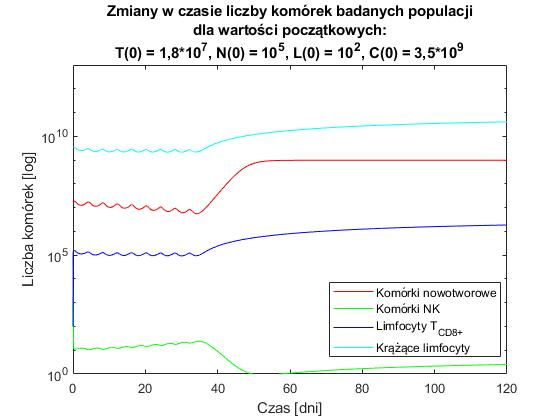
\includegraphics[width=0.5\textwidth]{wykres_chemio_zmiany_dawki}}
\quad
\subfloat[Zmiany w~czasie st�enia, dozowanego podczas chemioterapii, cytostatyka dla~4-dniowego cyklu chemioterapii oraz~dawki dozowanego cytostatyka $V_M = 3$ $\dfrac{mg}{m^{2}}$.]{\label{stezenie_chemio_zmiany_dawki}
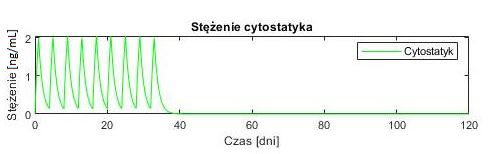
\includegraphics[width=0.5\textwidth]{stezenie_chemio_zmiany_dawki}}
\caption[Zmiany w~czasie liczby kom�rek badanych populacji oraz~st�enia cytostatyka - chemioterapia, scenariusz II, zmiana dawki dozowanego cytostatyka $V_M$]{Zmiany w~czasie liczby kom�rek badanych populacji oraz~st�enia dozowanego podczas chemioterapii cytostatyka dla~4-dniowego cyklu chemioterapii oraz~dawki dozowanego cytostatyka $V_M = 3$ $\dfrac{mg}{m^{2}}$. Pocz�tkowa liczba kom�rek nowotworowych $T(0) = 1,8 \cdot 10^{7}$, pocz�tkowa liczba kom�rek NK $N(0) = 10^{5}$, pocz�tkowa liczba limfocyt�w $T_{CD8+}$ $L(0) = 10^{2}$, pocz�tkowa liczba limfocyt�w kr���cych $C(0) = 3,5 \cdot 10^{9}$.}
\label{wykresy_chemio_zmiany_dawki}
\end{figure}

\newpage
Rys. \ref{dzien_regr_w_zaleznosci_od_dawki} przedstawia zale�no�� dnia wyst�pienia regresji nowotworu od~u�ytej dawki cytostatyka $V_M$. Powy�ej pewnego progu ($\sim 10$ $\dfrac{mg}{m^{2}}$) zwi�kszanie dawki nie~ma~wp�ywu na~przyspieszenie regresji.

\begin{figure}[h!]
\centering
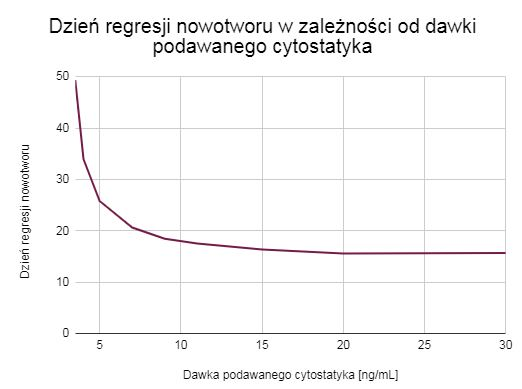
\includegraphics[width=0.65\textwidth]{dzien_regr_w_zaleznosci_od_dawki}
\caption{Dzie� regresji nowotworu w~zale�no�ci od~dawki dozowanego cytostatyka~$V_M$.}\label{dzien_regr_w_zaleznosci_od_dawki}
\end{figure}

Cz�� wynik�w symulacji w~formie graficznej, przedstawia Rys. \ref{slupki_7.3}.\\

\begin{figure}[h!]
\centering
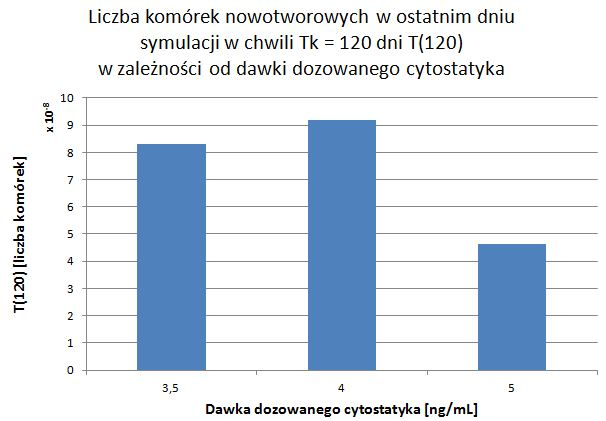
\includegraphics[width=0.8\textwidth]{slupki_7.3}
\caption{Liczba kom�rek nowotworowych $T(120)$  w ostatnim dniu symulacji w chwili $T_{k} = 120$ dni w zale�no�ci od dawki dozowanego cytostatyka $V_M$.}\label{slupki_7.3}
\end{figure}

\newpage
\textbf{Wnioski:}
\begin{itemize}
\item skuteczno�� chemioterapii (regresja nowotworu lub jej brak) oraz~czas potrzebny do~regresji nowotworu b�d�cej skutkiem chemioterapii zale�y od~dawki dozowanego podczas leczenia cytostatyka; regresja nowotworu nie~wyst�puje dla~dawki $V_M = 3$ $\dfrac{mg}{m^{2}}$, natomiast dla~dawki $V_M = 3,5$ $\dfrac{mg}{m^{2}}$ wyst�puje w~50 dniu od~rozpocz�cia symulacji (leczenia);
\item dla~niewielkich warto�ci dawki cytostatyka $V_M$ (np.: $V_M = 3,5$ $\dfrac{mg}{m^{2}}$, $V_M = 4$ $\dfrac{mg}{m^{2}}$, $V_M = 5$ $\dfrac{mg}{m^{2}}$) ma�e zmiany dawki powoduj� znaczne skr�cenie czasu potrzebnego do~regresji nowotworu (dzie� regresji, odpowiednio: 50, 34, 26), natomiast przy wi�kszych dawkach (np.: $V_M = 11$ $\dfrac{mg}{m^{2}}$, $V_M = 20$ $\dfrac{mg}{m^{2}}$, $V_M = 30$ $\dfrac{mg}{m^{2}}$), ich zmiana nie~wp�ywa znacz�co na~dzie� regresji (dzie� regresji, odpowiednio: 18, 16, 16);
\item skuteczna dawka cytostatyka r�ni si� w~zale�no�ci od~d�ugo�ci cyklu chemioterapii; dla~4-dniowego cyklu chemioterapii do~skutecznego leczenia wystarczaj�ca jest dawka $V_M = 3,5$ $\dfrac{mg}{m^{2}}$, przy dwukrotnie d�u�szym cyklu (8 dni) konieczna jest prawie 4 razy wi�ksza dawka ($V_M = 13$ $\dfrac{mg}{m^{2}}$), natomiast przy cyklu trzykrotnie d�u�szym (12 dni) jest ponad 15 razy wi�ksza ($V_M = 53$ $\dfrac{mg}{m^{2}}$).
\end{itemize}

Analiza zmian dawki podawanego cytostatyka $V_M$ wykaza�a, �e mo�liwe jest uzyskanie podobnych efekt�w leczenia przy wykorzystaniu ograniczonej ilo�ci szkodliwego dla~zdrowych kom�rek cytostatyka. Jedyn� r�nic� przy zmniejszaniu dawki $V_M$ jest wyd�u�ony czas terapii. Ponadto, wykazano, �e dla~danego cytostatyka powy�ej pewnego progu ($\sim 10$ $\dfrac{mg}{m^{2}}$) dalsze zwi�kszanie dawki $V_M$ nie~wp�ywa na~polepszenie skutk�w leczenia.

\newpage
\section{Scenariusz III -- zmiana dawki dozowanego cytostatyka $V_M$ w~kolejnych powt�rzeniach cyklu}
\noindent \textbf{Podejmowany problem:} \newline Wp�yw zmian dawki dozowanego cytostatyka $V_M$ w~kolejnych powt�rzeniach cyklu na~skuteczno�� terapii.

\noindent \newline \textbf{Warunki pocz�tkowe:} 
\begin{itemize}
\item dla~pocz�tkowej wielko�ci badanych populacji, tj. pocz�tkow� liczb� kom�rek nowotworu $T(0)$, liczb� kom�rek NK $N(0)$, liczb� limfocyt�w $T_{CD8+}$ oraz~liczb� limfocyt�w kr���cych $C(0)$ przedstawia Tab. \ref{warunki_poczatkowe_z1};
\item dla~chemioterapii, tj. d�ugo�� cyklu, czas dozowania cytostatyka, schemat cyklu, dawk� dozowanego cytostatyka $V_M$, liczb� powt�rze� cyklu oraz~dzie� rozpocz�cia chemioterapii przedstawia Tab.~\ref{warunki pocz�tkowe_chemioterapii}.
\end{itemize}

\noindent \newline \textbf{Przyj�te parametry:} \newline Parametry dla~modelu uwzgl�dniaj�cego leczenie przedstawia Tab. \ref{parametry_modelu_bez1} i~\ref{parametry_modelu_z1}.

\noindent \newline \textbf{Czas symulacji:} \newline Czas symulacji wynosi� $T_{k}$ = 120 dni. 

\noindent \newline \textbf{Wyniki symulacji:} \newline Wyniki przeprowadzonych symulacji dla~zmieniaj�cej si� dawki cytostatyka $V_M$ w~kolejnych powt�rzeniach cyklu zebrano w~Tab.~\ref{chemio_zmiany_dawki_w_kolejnych_powtorzeniach}.  \newline

Tab. \ref{chemio_zmiany_dawki_w_kolejnych_powtorzeniach} przedstawia zmiany dawki dozowanego cytostatyka $V_M$ w~kolejnych powt�rzeniach cyklu (w~ka�dym kolejnym cyklu zmniejszano dawk� $V_M$ o~podan� warto��, zaczynaj�c od~$V_M = 5$ $\dfrac{mg}{m^{2}}$). Dodatkowo, Tab. \ref{chemio_zmiany_dawki_w_kolejnych_powtorzeniach} przedstawia schemat cyklu, dzie� regresji nowotworu oraz~liczb� kom�rek nowotworu T(120) w~ostatnim (120) dniu symulacji, a~tak�e~szacowan� obj�to�� i~d�ugo�� promienia nowotworu w~ostatnim dniu symulacji (tj. w~chwili $T_{k}$ = 120 dni).

\begin{table}[h!]
\small
	\centering
	\caption[Wyniki symulacji - chemioterapia, scenariusz III, zmiana dawki dozowanego cytostatyka $V_M$ w~kolejnych powt�rzeniach cyklu]{Schemat cyklu chemioterapii, r�nica pomi�dzy kolejnymi dawkami (dawka $V_M$ zmniejszana z~ka�dym kolejnym powt�rzeniem cyklu o~podan� w~tabeli warto��, zaczynaj�c od~$V_M = 5$ $\dfrac{mg}{m^{2}}$) dozowanego cytostatyka $V_M$, dzie� regresji nowotworu, liczba kom�rek nowotworowych T(120) w~ostatnim dniu symulacji oraz~szacowana obj�to�� i~d�ugo�� promienia nowotworu w~ostatnim dniu symulacji (tj. w~chwili $T_{k}$~=~120~dni).}
\label{chemio_zmiany_dawki_w_kolejnych_powtorzeniach}
\begin{tabular}{|c|c|c|c|c|c|} \hline
		Schemat & Dawka & Dzie� & $T(120)$ & Obj�to�� & D�ugo�� \\
		cyklu & dozowanego & regresji & $[liczba$ & nowotworu & promienia \\ 
		& cytostatyka & nowotworu & $kom$�$rek]$ & [$mm^{3}$] & nowotworu [$mm$] \\ 
		& $V_M$ $[\dfrac{mg}{m^{2}}]$ & & & & \\ \hline
		[1 3] & $0,1$ & 26,84 & $1,53 \cdot 10^{-7}$ & $1,53 \cdot 10^{-13}$ & $3,3 \cdot 10^{-5}$ \\ \hline
		[1 3] & $0,2$ & 27,96 & $3,13 \cdot 10^{-8}$ & $3,13 \cdot 10^{-14}$ & $2 \cdot 10^{-5}$ \\ \hline
		[1 3] & $0,3$ & 29,34 & $4,25 \cdot 10^{-8}$ & $4,25 \cdot 10^{-14}$ & $2,2 \cdot 10^{-5}$ \\ \hline
		[1 3] & $0,4$ & 33,04 & $2,04 \cdot 10^{-7}$ & $2,04 \cdot 10^{-13}$ & $3,7 \cdot 10^{-5}$ \\ \hline
		[1 3] & $0,5$ & brak & $9,8 \cdot 10^{8}$ & $980$ & $6,16$ \\ \hline
		\end{tabular}
\end{table} 

\newpage
Przyk�adowo, Rys. \ref{wykresy_chemio_zmiany_dawki_w_kolejnych_powtorzeniach4} przedstawia zmiany w~czasie liczby kom�rek badanych populacji, tj. kom�rek nowotworowych, kom�rek NK, limfocyt�w $T_{CD8+}$ oraz~limfocyt�w kr���cych dla~4-dniowego cyklu chemioterapii oraz~dawki dozowanego cytostatyka $V_M$ zmniejszanej w~kolejnych powt�rzeniach o~$0,4$ $\dfrac{mg}{m^{2}}$ (Rys.~\ref{wykres_chemio_zmiany_dawki_w_kolejnych_powtorzeniach4}) oraz~o~$0,5$~(Rys.~\ref{wykres_chemio_zmiany_dawki_w_kolejnych_powtorzeniach5}), a~tak�e zmiany w~czasie st�enia (Rys.~\ref{stezenie_chemio_zmiany_dawki_w_kolejnych_powtorzeniach4} oraz~Rys. \ref{stezenie_chemio_zmiany_dawki_w_kolejnych_powtorzeniach5}), dozowanego podczas chemioterapii, cytostatyka. 

Symulacja zak�ada�a rozpocz�cie chemioterapii w~pierwszym dniu symulacji i~dziewi�ciokrotne powt�rzenie cyklu, przy czym w~ka�dym kolejnym powt�rzeniu dawka $V_M$ zmniejszana by�a odpowiednio o~$0,4$ $\dfrac{mg}{m^{2}}$ i~$0,5$ $\dfrac{mg}{m^{2}}$, rozpoczynaj�c od~dawki pocz�tkowej $V_M = 5$ $\dfrac{mg}{m^{2}}$. Czas podawania cytostatyka wynosi� 1 dzie� (24 godziny), natomiast d�ugo�� przerwy pomi�dzy kolejnymi powt�rzeniami wynosi�a 3 dni. 

\newpage
Zmniejszanie dawki $V_M$ o~$0,4$ $\dfrac{mg}{m^{2}}$ pozwoli�o ograniczy� negatywne skutki dzia�ania cytostatyka przy jednoczesnym zachowaniu skuteczno�ci leczenia (regresja nowotworu po~34 dniach (Rys. \ref{wykres_chemio_zmiany_dawki_w_kolejnych_powtorzeniach4})). W przypadku zmniejszania dawki $V_M$ o~$0,5$ $\dfrac{mg}{m^{2}}$ regresja nie~nast�pi�a, a~liczba kom�rek nowotworowych w~67 dniu symulacji (Rys. \ref{wykres_chemio_zmiany_dawki_w_kolejnych_powtorzeniach5}) ustabilizowa�a si� na~wysokim poziomie ($9,8 \cdot 10^{8}$).  

\begin{figure}[h!]
\centering
\subfloat[Zmiany w~czasie liczby kom�rek badanych populacji dla~dawki dozowanego cytostatyka $V_M$ zmniejszanej w~kolejnych powt�rzeniach o~$0,4$ $\dfrac{mg}{m^{2}}$. Widoczna (linia czerwona) regresja nowotworu po~34 dniach.]{\label{wykres_chemio_zmiany_dawki_w_kolejnych_powtorzeniach4}
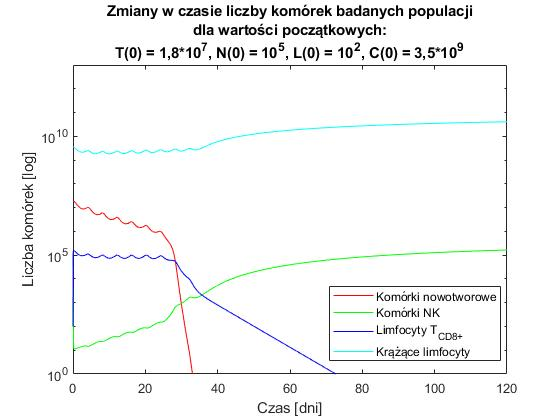
\includegraphics[width=0.45\textwidth]{wykres_chemio_zmiany_dawki_w_kolejnych_powtorzeniach4}}
\quad
\subfloat[Zmiany w~czasie liczby kom�rek badanych populacji dla~dawki dozowanego cytostatyka $V_M$ zmniejszanej w~kolejnych powt�rzeniach o~$0,5$ $\dfrac{mg}{m^{2}}$. Widoczna (linia czerwona) stabilizacja liczby kom�rek nowotworowych po~67 dniach oko�o warto�ci $9,8 \cdot 10^{8}$.]{\label{wykres_chemio_zmiany_dawki_w_kolejnych_powtorzeniach5}
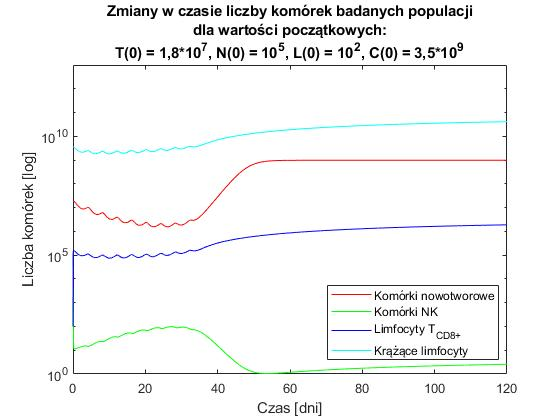
\includegraphics[width=0.45\textwidth]{wykres_chemio_zmiany_dawki_w_kolejnych_powtorzeniach5}}
\quad
\subfloat[Zmiany w~czasie st�enia, dozowanego podczas chemioterapii, cytostatyka dla~dawki dozowanego cytostatyka $V_M$ zmniejszanej w~kolejnych powt�rzeniach o~$0,4$ $\dfrac{mg}{m^{2}}$.]{\label{stezenie_chemio_zmiany_dawki_w_kolejnych_powtorzeniach4}
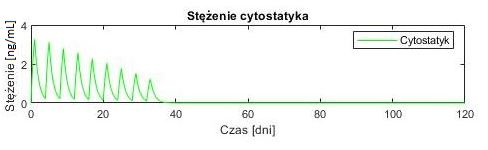
\includegraphics[width=0.45\textwidth]{stezenie_chemio_zmiany_dawki_w_kolejnych_powtorzeniach4}}
\quad
\subfloat[Zmiany w~czasie st�enia, dozowanego podczas chemioterapii, cytostatyka dla~dawki dozowanego cytostatyka $V_M$ zmniejszanej w~kolejnych powt�rzeniach o~$0,5$ $\dfrac{mg}{m^{2}}$.]{\label{stezenie_chemio_zmiany_dawki_w_kolejnych_powtorzeniach5}
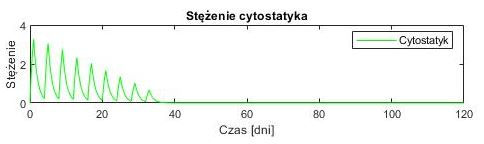
\includegraphics[width=0.45\textwidth]{stezenie_chemio_zmiany_dawki_w_kolejnych_powtorzeniach5}}
\caption[Zmiany w~czasie liczby kom�rek badanych populacji oraz~st�enia cytostatyka - chemioterapia, scenariusz III, zmiana dawki dozowanego cytostatyka $V_M$ w~kolejnych powt�rzeniach cyklu]{Zmiany w~czasie liczby kom�rek badanych populacji oraz~st�enia dozowanego podczas chemioterapii cytostatyka dla~dawki dozowanego cytostatyka $V_M$ zmniejszanej w~kolejnych powt�rzeniach o~$0,4$ $\dfrac{mg}{m^{2}}$ i~$0,5$ $\dfrac{mg}{m^{2}}$. Pocz�tkowa liczba kom�rek nowotworowych $T(0) = 1,8 \cdot 10^{7}$, pocz�tkowa liczba kom�rek NK $N(0) = 10^{5}$, pocz�tkowa liczba limfocyt�w $T_{CD8+}$ $L(0) = 10^{2}$, pocz�tkowa liczba limfocyt�w kr���cych $C(0) = 3,5 \cdot 10^{9}$.}
\label{wykresy_chemio_zmiany_dawki_w_kolejnych_powtorzeniach4}
\end{figure}

\newpage
\textbf{Wnioski:}
\begin{itemize}
\item chemioterapia jest skuteczna (wyst�puje regresja nowotworu) w~przypadku zmniejszania wielko�ci dawki z~ka�dym kolejnym cyklem; leczenie metod� chemioterapii przy sta�ej dawce cytostatyka $V_M = 4$ $\dfrac{mg}{m^{2}}$ (dzie� regresji: 34, Tab. \ref{chemio_zmiany_dawki}) ma~czas potrzebny do~wyst�pienia regresji nowotworu por�wnywalny do~leczenia ze zmniejszaniem dawki $V_M$ o~0,4 $\dfrac{mg}{m^{2}}$ w~kolejnych cyklach rozpoczynaj�c od~$V_M = 5$ $\dfrac{mg}{m^{2}}$ (dzie� regresji: 34); w~pierwszym przypadku regresja zostaje osi�gni�ta poprzez dziewi�ciokrotne u�ycie takiej samej dawki $V_M = 4$ $\dfrac{mg}{m^{2}}$, podczas gdy w~drugim przypadku wykorzystane s�~3 wi�ksze oraz~6 mniejszych dawek, co~pozwala osi�gn�� ten~sam efekt przy mniejszej sumarycznej dawce cytostatyka przyjmowanej przez~pacjenta, tj. mniejszych skutkach ubocznych.
\end{itemize}

Poza analiz� dawek cytostatyka o~sta�ej warto�ci przez~ca�y czas trwania leczenia, testowano r�wnie�~zmniejszanie dawki w~kolejnych powt�rzeniach cyklu. Z~symulacji wynika, �e mo�e to~by� spos�b na~ograniczenie przyjmowanego przez~pacjenta szkodliwego cytostatyka. 

\newpage
\section{Scenariusz IV -- zmiana liczby powt�rze� cyklu}
\noindent \textbf{Podejmowany problem:} \newline Wp�yw zmian liczby powt�rze� cyklu chemioterapii na skuteczno�� terapii.

\noindent \newline \textbf{Warunki pocz�tkowe:} 
\begin{itemize}
\item dla~pocz�tkowej wielko�ci badanych populacji, tj. pocz�tkow� liczb� kom�rek nowotworu $T(0)$, liczb� kom�rek NK $N(0)$, liczb� limfocyt�w $T_{CD8+}$ oraz~liczb� limfocyt�w kr���cych $C(0)$ przedstawia Tab. \ref{warunki_poczatkowe_z1};
\item dla~chemioterapii, tj. d�ugo�� cyklu, czas dozowania cytostatyka, schemat cyklu, liczb� powt�rze� cyklu oraz~dzie� rozpocz�cia chemioterapii przedstawia Tab.~\ref{warunki pocz�tkowe_chemioterapii}. Dawka dozowanego cytostatyka $V_M$ wynosi�a 5 $\dfrac{mg}{m^{2}}$, 4 $\dfrac{mg}{m^{2}}$, 3,5 $\dfrac{mg}{m^{2}}$ oraz~3 $\dfrac{mg}{m^{2}}$.
\end{itemize}

\noindent \newline \textbf{Przyj�te parametry:} \newline Parametry dla~modelu uwzgl�dniaj�cego leczenie przedstawia Tab. \ref{parametry_modelu_bez1} i~\ref{parametry_modelu_z1}.

\noindent \newline \textbf{Czas symulacji:} \newline Czas symulacji wynosi� $T_{k}$ = 120 dni. 

\noindent \newline \textbf{Wyniki symulacji:} \newline Wyniki przeprowadzonych symulacji dla~zmieniaj�cej si� liczby powt�rze� cyklu chemioterapii zebrano w~Tab. \ref{chemio_zmiany_liczby_powtorzen}. \newline

Tab. \ref{chemio_zmiany_liczby_powtorzen} przedstawia zmiany liczby powt�rze� cyklu. Dodatkowo, umieszczono w~Tab. \ref{chemio_zmiany_liczby_powtorzen} schemat cyklu, dzie� regresji nowotworu oraz~liczb� kom�rek nowotworu T(120) w~ostatnim (120) dniu symulacji, a~tak�e~szacowan� obj�to�� i~d�ugo�� promienia nowotworu w~ostatnim (120) dniu symulacji (tj. w~chwili $T_{k}$ = 120 dni). Analiz� przeprowadzono dla~dawki dozowanego cytostatyka $V_M$ r�wnej 5 $\dfrac{mg}{m^{2}}$, 4 $\dfrac{mg}{m^{2}}$, 3,5 $\dfrac{mg}{m^{2}}$ oraz~3 $\dfrac{mg}{m^{2}}$.

\newpage
\begin{table}[h!]
\small
	\centering
	\caption[Wyniki symulacji - chemioterapia, scenariusz IV, zmiana liczby powt�rze� cyklu chemioterapii]{Schemat oraz~liczba powt�rze� cyklu chemioterapii, dzie� regresji nowotworu, liczba kom�rek nowotworowych T(120) w~ostatnim (120) dniu symulacji oraz~szacowana obj�to�� i~d�ugo�� promienia nowotworu w~ostatnim (120) dniu symulacji (tj. w~chwili $T_{k}$ = 120 dni) dla~dawki dozowanego cytostatyka $V_M$ r�wnej 5 $\dfrac{mg}{m^{2}}$, 4 $\dfrac{mg}{m^{2}}$, 3,5~$\dfrac{mg}{m^{2}}$ oraz~3 $\dfrac{mg}{m^{2}}$.}
\label{chemio_zmiany_liczby_powtorzen}
\begin{tabular}{|c|c|c|c|c|c|} \hline \hline
        \multicolumn{6}{|c|}{\textbf{$V_M = 5$ $\dfrac{mg}{m^{2}}$}} \\ \hline \hline
		Schemat & Liczba & Dzie� & $T(120)$ & Obj�to�� & D�ugo��  \\
		cyklu & powt�rze� & regresji & $[liczba$ & nowotworu & promienia \\ 
		& cyklu & nowotworu & $kom$�$rek]$ & [$mm^{3}$] & nowotworu [$mm$]\\ \hline
		[1 3] & 9 & 25,84 & $4,64 \cdot 10^{-8}$ & $4,64 \cdot 10^{-14}$ & $2,2 \cdot 10^{-5}$ \\ \hline
		[1 3] & 8 & 25,84 & $1,32 \cdot 10^{-7}$ & $1,32 \cdot 10^{-13}$ & $3,2 \cdot 10^{-5}$ \\ \hline
		[1 3] & 7 & 25,84 & $2 \cdot 10^{-7}$ & $2 \cdot 10^{-13}$ & $3,6 \cdot 10^{-5}$ \\ \hline
		[1 3] & 6 & 26,5 & $6,08 \cdot 10^{-8}$ & $6,08 \cdot 10^{-14}$ & $2,4 \cdot 10^{-5}$ \\ \hline
		[1 3] & 5 & 27,92 & $2,31 \cdot 10^{-8}$ & $2,31 \cdot 10^{-14}$ & $1,8 \cdot 10^{-5}$ \\ \hline
		[1 3] & 4 & brak & $9,8 \cdot 10^{8}$ & $980$ & $6,16$ \\ \hline \hline
        \multicolumn{6}{|c|}{\textbf{$V_M = 4$ $\dfrac{mg}{m^{2}}$}} \\ \hline \hline
		Schemat & Liczba & Dzie� & $T(120)$ & Obj�to�� & D�ugo��  \\
		cyklu & powt�rze� & regresji & $[liczba$ & nowotworu & promienia \\ 
		& cyklu & nowotworu & $kom$�$rek]$ & [$mm^{3}$] & nowotworu [$mm$]\\ \hline
		[1 3] & 9 & 34 & $9,18 \cdot 10^{-8}$ & $9,18 \cdot 10^{-14}$ & $2,8 \cdot 10^{-5}$ \\ \hline
		[1 3] & 8 & 34,67 & $1,19 \cdot 10^{-7}$ & $1,19 \cdot 10^{-13}$ & $3,1 \cdot 10^{-5}$ \\ \hline
		[1 3] & 7 & 36,04 & $5,37 \cdot 10^{-8}$ & $5,37 \cdot 10^{-14}$ & $2,3 \cdot 10^{-5}$ \\ \hline
		[1 3] & 6 & brak & $9,8 \cdot 10^{8}$ & $980$ & $6,16$ \\ \hline  \hline
		 \multicolumn{6}{|c|}{\textbf{$V_M = 3,5$} $\dfrac{mg}{m^{2}}$} \\ \hline \hline
		Schemat & Liczba & Dzie� & $T(120)$ & Obj�to�� & D�ugo��  \\
		cyklu & powt�rze� & regresji & $[liczba$ & nowotworu & promienia \\ 
		& cyklu & nowotworu & $kom$�$rek]$ & [$mm^{3}$] & nowotworu [$mm$]\\ \hline
		[1 3] & 9 & 49,34 & $8,32 \cdot 10^{-8}$ & $8,32 \cdot 10^{-14}$ & $2,7 \cdot 10^{-5}$ \\ \hline
		[1 3] & 8 & brak & $9,8 \cdot 10^{8}$ & $980$ & $6,16$ \\ \hline  \hline
		 \multicolumn{6}{|c|}{\textbf{$V_M = 3$ $\dfrac{mg}{m^{2}}$}} \\ \hline \hline
		Schemat & Liczba & Dzie� & $T(120)$ & Obj�to�� & D�ugo��  \\
		cyklu & powt�rze� & regresji & $[liczba$ & nowotworu & promienia \\ 
		& cyklu & nowotworu & $kom$�$rek]$ & [$mm^{3}$] & nowotworu [$mm$]\\ \hline
		[1 3] & 9 & brak & $9,8 \cdot 10^{8}$ & $980$ & $6,16$ \\ \hline
		[1 3] & 15 & brak & $9,8 \cdot 10^{8}$ & $980$ & $6,16$ \\ \hline
		[1 3] & 19 & 86,92 & $1,37 \cdot 10^{-7}$ & $1,37 \cdot 10^{-13}$ & $3,2 \cdot 10^{-5}$  \\ \hline
		[1 3] & 20 & 84,5 & $6,8 \cdot 10^{-8}$ & $6,8 \cdot 10^{-14}$ & $2,5 \cdot 10^{-5}$  \\ \hline
		\end{tabular}
\end{table} 

\newpage 
Przyk�adowo, Rys. \ref{wykresy_chemio_zmiany_liczby_powtorzen4} ukazuje zmiany w~czasie liczby kom�rek badanych populacji, tj. kom�rek nowotworowych, kom�rek NK, limfocyt�w $T_{CD8+}$ oraz~limfocyt�w kr���cych 4-dniowego cyklu chemioterapii oraz~4 powt�rze� cyklu (Rys. \ref{wykres_chemio_zmiany_liczby_powtorzen4}), a~tak�e zmiany w~czasie st�enia, dozowanego podczas chemioterapii, cytostatyka (Rys. \ref{stezenie_chemio_zmiany_liczby_powtorzen4}). 

Za�o�ono dawk� $V_M = 5$~$\dfrac{mg}{m^{2}}$ oraz~rozpocz�cie chemioterapii pierwszego dnia symulacji. Czas podawania cytostatyka wynosi� 1 dzie� (24 godziny), natomiast d�ugo�� przerwy pomi�dzy kolejnymi powt�rzeniami wynosi�a 3 dni. 

Ograniczenie liczby powt�rze� cyklu do~4 uniemo�liwi�o uzyskanie regresji guza. Po zako�czeniu leczenia liczba kom�rek nowotworowych wzros�a i~ustabilizowa�a si� na~wysokim poziomie ($9,8 \cdot 10^{8}$) w~52 dniu symulacji (Rys. \ref{wykres_chemio_zmiany_liczby_powtorzen4}).  

\begin{figure}[h!]
\centering
\subfloat[Zmiany w~czasie liczby kom�rek badanych populacji dla~4-dniowego cyklu chemioterapii oraz~liczby powt�rze� cyklu wynosz�cej 4. Widoczna (linia czerwona) stabilizacja liczby kom�rek nowotworowych po~czasie 52 dniach oko�o warto�ci $9,8 \cdot 10^{8}$.]{\label{wykres_chemio_zmiany_liczby_powtorzen4}
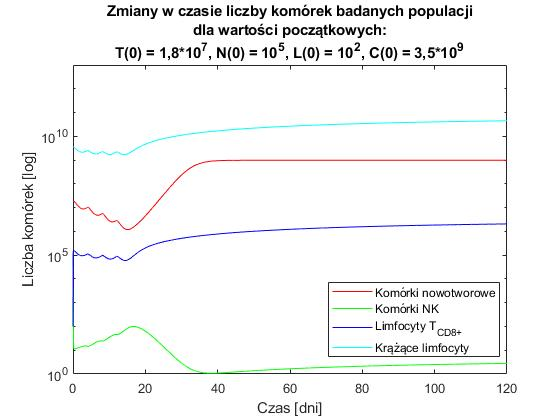
\includegraphics[width=0.5\textwidth]{wykres_chemio_zmiany_liczby_powtorzen4}}
\quad
\subfloat[Zmiany w~czasie st�enia, dozowanego podczas chemioterapii, cytostatyka dla~4-dniowego cyklu chemioterapii oraz~liczby powt�rze� cyklu wynosz�cej 4.]{\label{stezenie_chemio_zmiany_liczby_powtorzen4}
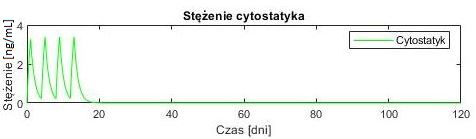
\includegraphics[width=0.5\textwidth]{stezenie_chemio_zmiany_liczby_powtorzen4}}
\caption[Zmiany w~czasie liczby kom�rek badanych populacji oraz~st�enia cytostatyka - chemioterapia, scenariusz IV, zmiana liczby powt�rze� cyklu chemioterapii]{Zmiany w~czasie liczby kom�rek badanych populacji oraz~st�enia dozowanego podczas chemioterapii cytostatyka dla~4-dniowego cyklu chemioterapii oraz~liczby powt�rze� cyklu wynosz�cej 4. Pocz�tkowa liczba kom�rek nowotworu $T(0) = 1,8 \cdot 10^{7}$, pocz�tkowa liczba kom�rek NK $N(0) = 10^{5}$, pocz�tkowa liczba limfocyt�w $T_{CD8+}$ $L(0) = 10^{2}$, pocz�tkowa liczba limfocyt�w kr���cych $C(0) = 3,5 \cdot 10^{9}$.}
\label{wykresy_chemio_zmiany_liczby_powtorzen4}
\end{figure}

\newpage
\textbf{Wnioski:}
\begin{itemize}
\item skuteczno�� chemioterapii (regresja nowotworu) zale�y od~liczby powt�rze� cyklu chemioterapii; dla~dawki cytostatyka $V_M = 5$ $\dfrac{mg}{m^{2}}$ leczenie jest skuteczne (dzie� regresji: 28) przy 5 powt�rzeniach cyklu, natomiast przy wi�kszej liczbie powt�rze� (6, 7 powt�rze�) moment wyst�pienia regresji nowotworu nast�puje nieznacznie wcze�niej (dzie� regresji: 27, 26) lub w~tym samym czasie (8, 9 powt�rze� - dzie� regresji: 26, 26);
\item chemioterapia przy u�yciu dawki $V_M = 3$ $\dfrac{mg}{m^{2}}$, kt�ra nie~jest skuteczna dla~9 powt�rze� cyklu (brak regresji nowotworu) przy wi�kszej ilo�ci powt�rze� cyklu (19 powt�rze�) pozwala osi�gn�� pozytywny wynik leczenia; czas do~wyst�pienia regresji wynosi w~tym przypadku 87 dni (ponad 3 razy wi�cej ni�~przy 5 powt�rzeniach i~dawce $V_M = 5$ $\dfrac{mg}{m^{2}}$), ale~jest to~mo�liwo�� zastosowania chemioterapii u~pacjent�w, kt�rych organizm jest zbyt wyniszczony, by~zastosowa� wi�ksz� dawk� cytostatyka $V_M$.
\end{itemize}

Zgodnie z~przeprowadzon� analiz� zmian liczby powt�rze� cyklu mo�na stwierdzi�, �e leczenie metod� chemioterapii jest procesem z�o�onym, w~kt�rym jednym z istotnych czynnik�w jest okre�lenie ile razy nale�y powt�rzy� dozowanie cytostatyka u~danego pacjenta. Symulacje umo�liwiaj� wyznaczenie momentu, w~kt�rym dzia�anie cytostatyka obni�a liczb� kom�rek nowotworowych do~takiej warto�ci, przy kt�rej guz ulega regresji i~nie zaczyna na~nowo wzrasta�.

\newpage
\section{Scenariusz V -- zmiana dnia rozpocz�cia chemioterapii}
\noindent \textbf{Podejmowany problem:} \newline Wp�yw zmian dnia rozpocz�cia chemioterapii (dozowania cytostatyka) na~skuteczno�� terapii.

\noindent \newline \textbf{Warunki pocz�tkowe:} 
\begin{itemize}
\item dla~pocz�tkowej wielko�ci badanych populacji, tj. pocz�tkow� liczb� kom�rek nowotworu $T(0)$, liczb� kom�rek NK $N(0)$, liczb� limfocyt�w $T_{CD8+}$ oraz~liczb� limfocyt�w kr���cych $C(0)$ przedstawia Tab. \ref{warunki_poczatkowe_z1};
\item dla~chemioterapii, tj. d�ugo�� cyklu, czas dozowania cytostatyka, schemat cyklu, liczb� powt�rze� cyklu oraz~dzie� rozpocz�cia chemioterapii przedstawia Tab.~\ref{warunki pocz�tkowe_chemioterapii}. Dawka dozowanego cytostatyka $V_M$ wynosi�a 5 $\dfrac{mg}{m^{2}}$ oraz~4,5 $\dfrac{mg}{m^{2}}$.
\end{itemize}

\noindent \newline \textbf{Przyj�te parametry:} \newline Parametry dla~modelu uwzgl�dniaj�cego leczenie przedstawia Tab. \ref{parametry_modelu_bez1} i~\ref{parametry_modelu_z1}.

\noindent \newline \textbf{Czas symulacji:} \newline Czas symulacji wynosi� $T_{k}$ = 120 dni. 

\noindent \newline \textbf{Wyniki symulacji:} \newline Wyniki przeprowadzonych symulacji dla~zmieniaj�cego si� dnia rozpocz�cia chemioterapii (dozowania cytostatyka) zebrano w~Tab. \ref{zmiany_dnia_rozpoczecia_cehmioterapii}. \newline

Tab. \ref{zmiany_dnia_rozpoczecia_cehmioterapii} przedstawia zmiany dnia rozpocz�cia chemioterapii. Dodatkowo, w~Tab. \ref{zmiany_dnia_rozpoczecia_cehmioterapii} umieszczono schemat cyklu, dzie� regresji nowotworu oraz~liczb� kom�rek nowotworu T(120) w~ostatnim (120) dniu symulacji, a~tak�e~szacowan� obj�to�� i~d�ugo�� promienia nowotworu w~ostatnim (120) dniu symulacji (tj. w~chwili $T_{k}$ = 120 dni). Analiz� przeprowadzono dla~dawki dozowanego cytostatyka $V_M$ r�wnej 5 $\dfrac{mg}{m^{2}}$ oraz~4,5~$\dfrac{mg}{m^{2}}$.

\newpage
\begin{table}[h!]
	\centering
	\caption[Wyniki symulacji - chemioterapia, scenariusz V, zmiana dnia rozpocz�cia chemioterapii]{Schemat cyklu oraz~dzie� rozpocz�cia chemioterapii, dzie� regresji nowotworu, liczba kom�rek nowotworowych T(120) w~ostatnim (120) dniu symulacji oraz~szacowana obj�to�� i~d�ugo�� promienia nowotworu w~ostatnim (120) dniu symulacji (tj. w~chwili $T_{k}$ = 120 dni) dla~dawki dozowanego cytostatyka $V_M$ r�wnej 5 $\dfrac{mg}{m^{2}}$ oraz~4,5~$\dfrac{mg}{m^{2}}$.}
\label{zmiany_dnia_rozpoczecia_cehmioterapii}
\begin{tabular}{|c|c|c|c|c|c|} \hline \hline
        \multicolumn{6}{|c|}{\textbf{$V_M = 5$ $\dfrac{mg}{m^{2}}$}} \\ \hline \hline
		Schemat & Dzie� & Dzie� & $T(120)$ & Obj�to�� & D�ugo�� \\
		cyklu & rozpocz�cia & regresji & $[liczba$ & nowotworu & promienia \\
		& chemioterapii & nowotworu & $kom$�$rek]$ & [$mm^{3}$] & nowotworu [$mm$] \\ \hline
		[1 3] & 1 & 25,84 & $4,64 \cdot 10^{-8}$ & $4,64 \cdot 10^{-14}$ & $2,2 \cdot 10^{-5}$ \\ \hline
		[1 3] & 2 & 29,54 & $2,29 \cdot 10^{-8}$ & $2,29 \cdot 10^{-14}$ & $1,8 \cdot 10^{-5}$ \\ \hline
		[1 3] & 5 & 39,84 & $1,79 \cdot 10^{-7}$ & $1,79 \cdot 10^{-13}$ & $3,5 \cdot 10^{-5}$ \\ \hline
		[1 3] & 11 & 59,25 & $2,61 \cdot 10^{-7}$ & $2,61 \cdot 10^{-13}$ & $4 \cdot 10^{-5}$ \\ \hline
		[1 3] & 12 & 60 & $3,93 \cdot 10^{-8}$ & $3,93 \cdot 10^{-14}$ & $2,1 \cdot 10^{-5}$ \\ \hline
		[1 3] & 13 & brak & $9,8 \cdot 10^{8}$ & $980$ & $6,16$ \\ \hline \hline
        \multicolumn{6}{|c|}{\textbf{$V_M = 4,5$ $\dfrac{mg}{m^{2}}$}} \\ \hline \hline
		Schemat & Dzie� & Dzie� & $T(120)$ & Obj�to�� & D�ugo�� \\
		cyklu & rozpocz�cia & regresji & $[liczba$ & nowotworu & promienia \\
		& chemioterapii & nowotworu & $kom$�$rek]$ & [$mm^{3}$] & nowotworu [$mm$] \\ \hline
		[1 3] & 1 & 28,46 & $9,03 \cdot 10^{-8}$ & $9,03 \cdot 10^{-14}$ & $2,8 \cdot 10^{-5}$ \\ \hline
		[1 3] & 2 & 31,92 & $8,87 \cdot 10^{-8}$ & $8,87 \cdot 10^{-14}$ & $2,8 \cdot 10^{-5}$ \\ \hline
		[1 3] & 3 & 37,38 & $1,72 \cdot 10^{-7}$ & $1,72 \cdot 10^{-13}$ & $3,5 \cdot 10^{-5}$ \\ \hline
		[1 3] & 4 & 43,54 & $2,66 \cdot 10^{-7}$ & $2,66 \cdot 10^{-13}$ & $4 \cdot 10^{-5}$ \\ \hline
		[1 3] & 5 & 49,84 & $1,75 \cdot 10^{-7}$ & $1,75 \cdot 10^{-13}$ & $3,5 \cdot 10^{-5}$ \\ \hline
		[1 3] & 6 & brak & $9,8 \cdot 10^{8}$ & $980$ & $6,16$ \\ \hline
		[1 3] & 7 & brak & $9,8 \cdot 10^{8}$ & $980$ & $6,16$ \\ \hline
		\end{tabular}
\end{table} 

Przyk�adowo, Rys. \ref{wykresy_zmiany_dnia_rozpoczecia_cehmioterapii13} przedstawia zmiany w~czasie liczby kom�rek badanych populacji, tj. kom�rek nowotworowych, kom�rek NK, limfocyt�w $T_{CD8+}$ oraz~limfocyt�w kr���cych dla~4-dniowego cyklu chemioterapii, rozpocz�tej w~13 dniu symulacji (Rys. \ref{wykres_zmiany_dnia_rozpoczecia_cehmioterapii13}), a~tak�e zmiany w~czasie st�enia, dozowanego podczas chemioterapii, cytostatyka (Rys. \ref{stezenie_zmiany_dnia_rozpoczecia_cehmioterapii13}). 

Symulacja zak�ada�a dziewi�ciokrotne powt�rzenie dozowania cytostatyka o~dawce $V_M = 5$ $\dfrac{mg}{m^{2}}$. Czas podawania cytostatyka wynosi� 1 dzie� (24 godziny), natomiast d�ugo�� przerwy pomi�dzy kolejnymi powt�rzeniami wynosi�a 3 dni. 

\newpage
Op�nienie leczenia o~nieca�e dwa tygodnie skutkowa�o rozrostem guza i~brakiem wyst�pienia regresji (Rys. \ref{wykres_zmiany_dnia_rozpoczecia_cehmioterapii13}). Liczba kom�rek nowotworowych ustabilizowa�a si� w~88 dniu symulacji na~wysokim poziomie ($9,8 \cdot 10^{8}$). 

\begin{figure}[h!]
\centering
\subfloat[Zmiany w~czasie liczby kom�rek badanych populacji dla~chemioterapii rozpocz�tej w~13 dniu. Widoczna (linia czerwona) stabilizacja liczby kom�rek nowotworowych po~czasie 88 dniach oko�o warto�ci $9,8 \cdot 10^{8}$.]{\label{wykres_zmiany_dnia_rozpoczecia_cehmioterapii13}
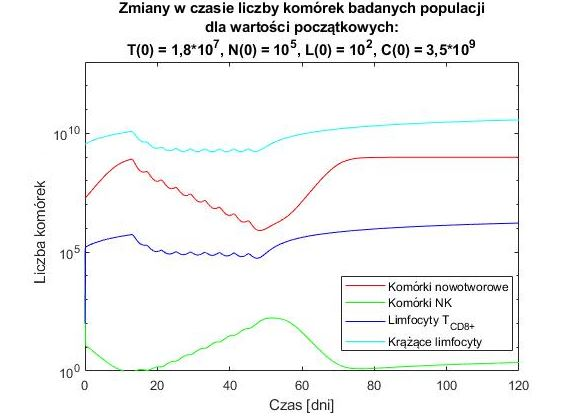
\includegraphics[width=0.5\textwidth]{wykres_zmiany_dnia_rozpoczecia_cehmioterapii13}}
\quad
\subfloat[Zmiany w~czasie st�enia, dozowanego podczas chemioterapii, cytostatyka dla~chemioterapii rozpocz�tej w~13 dniu.]{\label{stezenie_zmiany_dnia_rozpoczecia_cehmioterapii13}
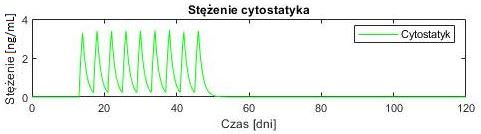
\includegraphics[width=0.5\textwidth]{stezenie_zmiany_dnia_rozpoczecia_cehmioterapii13}}
\caption[Zmiany w~czasie liczby kom�rek badanych populacji oraz~st�enia cytostatyka - chemioterapia, scenariusz V, zmiana dnia rozpocz�cia chemioterapii]{Zmiany w~czasie liczby kom�rek badanych populacji oraz~st�enia dozowanego podczas chemioterapii cytostatyka dla~chemioterapii rozpocz�tej w~13 dniu. Pocz�tkowa liczba kom�rek nowotworowych $T(0) = 1,8 \cdot 10^{7}$, pocz�tkowa liczba kom�rek NK $N(0) = 10^{5}$, pocz�tkowa liczba limfocyt�w $T_{CD8+}$ $L(0) = 10^{2}$, pocz�tkowa liczba limfocyt�w kr���cych $C(0) = 3,5 \cdot 10^{9}$.}
\label{wykresy_zmiany_dnia_rozpoczecia_cehmioterapii13}
\end{figure}

\newpage
Cz�� wynik�w symulacji w~formie graficznej, przedstawia Rys. \ref{slupki_7.5}.

\begin{figure}[h!]
\centering
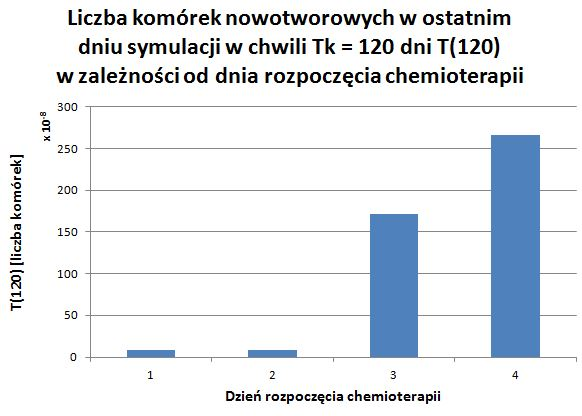
\includegraphics[width=0.8\textwidth]{slupki_7.5}
\caption{Liczba kom�rek nowotworowych $T(120)$  w ostatnim dniu symulacji w chwili $T_{k} = 120$ dni w zale�no�ci od dnia rozpocz�cia chemioterapii (dozowania cytostatyka).}\label{slupki_7.5}
\end{figure}

\textbf{Wnioski:}
\begin{itemize}
\item skuteczno�� chemioterapii (regresja nowotworu) zale�y od~dnia rozpocz�cia leczenia (dozowania cytostatyka); dla~dawki cytostatyka $V_M = 5$~$\dfrac{mg}{m^{2}}$ i~$V_M = 4,5$~$\dfrac{mg}{m^{2}}$ leczenie rozpocz�te w~1 dniu symulacji trwa odpowiednio: 26 dni oraz~29 dni (dzie� regresji nowotworu), podczas gdy rozpocz�te 4 dni p�niej trwa, odpowiednio 40 dni (o~2 tygodnie d�u�ej) oraz~50 dni (o~3 tygodnie d�u�ej);
\item dla~dawki $V_M = 4,5$ $\dfrac{mg}{m^{2}}$, przesuni�cie dnia rozpocz�cia chemioterapii zaledwie o~5 dni skutkuje negatywnym wynikiem leczenia (brakiem regresji nowotworu), podczas gdy dla dawki $V_M = 5$ $\dfrac{mg}{m^{2}}$ leczenie mo�na rozpocz�� nawet 12 dnia zachowuj�c skuteczno�� terapii, jednak ponad dwukrotnie (dzie� 60) wyd�u�aj�c czas do wyst�pienia regresji nowotworu.
\end{itemize}

Skuteczno�� chemioterapii w~du�ym stopniu zale�y od~dnia jej rozpocz�cia. Jak wynika z~symulacji, w~pewnych przypadkach, nawet niewielkie zmiany (np. op�nienie leczenia o~5 dni dla~dawki $V_M = 4,5$ $\dfrac{mg}{m^{2}}$) mog� decydowa� o~wyniku leczenia.

\newpage
\chapter{Leczenie metod� immunoterapii -- symulacje wykonane dla~modelu leczonego guza} \label{sym_i}

W symulacji leczenia metod� immunoterapii wzi�to pod uwag� takie zmienne, jak:
\begin{itemize}
\item wielko�� nowotworu (tj. liczba kom�rek nowotworowych) w~dniu rozpocz�cia immunoterapii,
\item dawk� interleukin-2 (IL-2) $V_I$,
\item dawk� limfocyt�w naciekaj�cych nowotw�r TIL (ang. Tumor Infiltrating Lymphocytes) $V_L$,
\item liczb� powt�rze� cyklu dawkowania IL-2,
\item dzie� rozpocz�cia immunoterapii (dozowania IL-2 lub TIL).
\end{itemize}

\begin{table}[h!]
	\centering
	\caption{Warunki pocz�tkowe modelu odpowiedzi immunologicznej na~rozwijaj�cy si� nowotw�r z~uwzgl�dnieniem procesu leczenia za~pomoc� immunoterapii.}\label{warunki_pocz�tkowe_immunoterapii}
\begin{tabular}{|c|c|c|c|c|c|} \hline \hline
        \multicolumn{6}{|c|}{\textbf{Lek: IL-2}} \\ \hline \hline
		D�ugo�� & Czas dozowania & Schemat & Dawka & Liczba & Dzie�  \\
		cyklu $[dni]$ & leku $[dni]$ & cyklu & IL-2 $V_I$ & powt�rze� & rozpocz�cia \\
		& & & $[\dfrac{IU}{kg}]$ & cyklu & immunoterapii \\ \hline
		0,5 & 0,3 & [0,3 0,2] & $5 \cdot 10^{6}$ & 6 & 9 \\ \hline \hline
		\multicolumn{6}{|c|}{\textbf{Lek: TIL}} \\ \hline \hline
		D�ugo�� & Czas dozowania & Schemat & Dawka & Liczba & Dzie�  \\
		cyklu $[dni]$ & leku $[dni]$ & cyklu & TIL $V_L$ & powt�rze� & rozpocz�cia \\
		& & & $[liczba$ & cyklu & immunoterapii \\ 
		& & & $kom$�$rek]$ & & \\ \hline
		1 & 1 & [1 0] & $1 \cdot 10^{9}$ & 1 & 8\\ \hline
		\end{tabular}
\end{table}

We~wszystkich symulacjach leczenia metod� immunoterapii analizowano zmiany odpowiedzi uk�adu immunologicznego (tj. liczby kom�rek nowotworowych oraz~kom�rek uk�adu odporno�ciowego) po~120 dniach ($T_{k} = 120$ dni) symulacji w~zale�no�ci od~wy�ej wymienionych zmiennych okre�laj�cych immunoterpi�.

\newpage
\section{Scenariusz I -- zmiana pocz�tkowej wielko�ci guza} \label{immuno_zmiana_pocz_war_guza}
\noindent \textbf{Podejmowany problem:} \newline Wp�yw zmian pocz�tkowej wielko�ci guza (liczby kom�rek nowotworowych) na~skuteczno�� terapii.

\noindent \newline \textbf{Warunki pocz�tkowe:} 
\begin{itemize}
\item dla~pocz�tkowej wielko�ci badanych populacji, tj. pocz�tkow� liczb� kom�rek nowotworu $T(0)$, liczb� kom�rek NK $N(0)$, liczb� limfocyt�w $T_{CD8+}$ oraz~liczb� limfocyt�w kr���cych $C(0)$ przedstawia Tab. \ref{warunki_poczatkowe_z1};
\item dla~immunoterapii, tj. d�ugo�� cyklu, czas dozowania, schemat cyklu, dawk� dozowanych lek�w (IL-2 i TIL), liczb� powt�rze� cyklu oraz~dzie� rozpocz�cia immunoterapii przedstawia Tab. \ref{warunki_pocz�tkowe_immunoterapii}.
\end{itemize}

\noindent \newline \textbf{Przyj�te parametry:} \newline Parametry dla~modelu uwzgl�dniaj�cego leczenie przedstawia Tab. \ref{parametry_modelu_bez1} i~\ref{parametry_modelu_z1}.

\noindent \newline \textbf{Czas symulacji:} \newline Czas symulacji wynosi� $T_{k}$ = 120 dni. 

\noindent \newline \textbf{Wyniki symulacji:} \newline Wyniki przeprowadzonych symulacji dla~zmieniaj�cej si� pocz�tkowej liczby kom�rek nowotworowych $T(0)$ zebrano w~Tab. \ref{immuno_zmiany_wielkosci_guza}. \newline

Tab. \ref{immuno_zmiany_wielkosci_guza} przedstawia zmiany pocz�tkow�ej liczby kom�rek nowotworowych $T(0)$. Dodatkowo, w~Tab. \ref{immuno_zmiany_wielkosci_guza} umieszczono dzie� regresji nowotworu oraz~liczb� kom�rek nowotworu T(120) w~ostatnim (120) dniu symulacji, a~tak�e~szacowan� obj�to�� i~d�ugo�� promienia nowotworu w~ostatnim (120) dniu symulacji (tj. w~chwili $T_{k}$ = 120 dni).

\begin{table}[h!]
\small
	\centering
	\caption[Wyniki symulacji - immunoterapia, scenariusz I, zmiana wielko�ci guza w~dniu rozpocz�cia immunoterapii]{Pocz�tkowa liczba kom�rek nowotworowych $T(0)$, dzie� regresji nowotworu, liczba kom�rek nowotworowych T(120) w~ostatnim (120) dniu symulacji oraz~szacowana obj�to�� i~d�ugo�� promienia nowotworu w~ostatnim (120) dniu symulacji (tj. w~chwili $T_{k}$ = 120 dni).}
\label{immuno_zmiany_wielkosci_guza}
\begin{tabular}{|c|c|c|c|c|} \hline
		$T(0)$  & Dzie� regresji & $T(120)$ & Obj�to�� & D�ugo�� \\
		$[liczba$ $kom$�$rek]$ & nowotworu & $[liczba$ $kom$�$rek]$ & nowotworu & promienia \\ 
		& & & [$mm^{3}$] & nowotworu [$mm$] \\ \hline
		$1 \cdot 10^{6}$ & 15,13 & $1,07 \cdot 10^{-87}$ & $1,07 \cdot 10^{-93}$ & $6,4 \cdot 10^{-32}$ \\ \hline
		$2 \cdot 10^{6}$ & 16,13 & $7,46 \cdot 10^{-87}$ & $7,46 \cdot 10^{-93}$ & $1,2 \cdot 10^{-31}$ \\ \hline
		$5 \cdot 10^{6}$ & 18,88 & $1,45 \cdot 10^{-84}$ & $1,45 \cdot 10^{-90}$ & $7 \cdot 10^{-31}$ \\ \hline
		$6 \cdot 10^{6}$ & brak & $9,8 \cdot 10^{8}$ & $980$ & $6,16$ \\ \hline
		$1 \cdot 10^{7}$ & brak & $9,8 \cdot 10^{8}$ & $980$ & $6,16$ \\ \hline
		$1,8 \cdot 10^{7}$ & brak & $9,8 \cdot 10^{8}$ & $980$ & $6,16$ \\ \hline
		\end{tabular}
\end{table} 

\newpage 
Przyk�adowo, Rys. \ref{wykresy_immuno_zmiany_wielkosci_guza} prezentuje zmiany w~czasie liczby kom�rek badanych populacji, tj. kom�rek nowotworowych, kom�rek NK, limfocyt�w $T_{CD8+}$ oraz~limfocyt�w kr���cych dla~immunoterapii, gdzie pocz�tkowa liczba kom�rek nowotworowych $T(0) = 10^{6}$ (Rys. \ref{wykres_immuno_zmiany_wielkosci_guza1e6}) oraz~$T(0) = 1,8 \cdot 10^{7}$ (Rys. \ref{wykres_immuno_zmiany_wielkosci_guza18e7}), a~tak�e zmiany w~czasie st�enia, dozowanych podczas immunoterapii, IL-2 (Rys. \ref{stezenie_immuno_zmiany_wielkosci_guza1e6}). 

Symulacja zak�ada�a sze�ciokrotny cykl dozowania IL-2 o~dawce $V_I = 5 \cdot 10^{6}$ $\dfrac{IU}{kg}$ oraz~jednokrotny cykl podawania TIL o~dawce $V_L = 10^{9}$ kom�rek. 

Czas dawkowania IL-2 wynosi� 7 godzin i~12 minut, natomiast czas dozowania TIL wynosi� 1 dzie� (24 godziny). D�ugo�� przerwy pomi�dzy kolejnymi powt�rzeniami cyklu IL-2 wynosi�a 4 godziny i~48 minut. Dzie� rozpocz�cia dozowania IL-2 to~9 dzie� symulacji, natomiast rozpocz�cie dozowania TIL nast�pi�o w~8 dniu symulacji. 

Immunoterapia by�a skuteczna w~przypadku niewielkiego guza ($T(0) = 10^{6}$), spowodowa�a regresj� w~16 dniu symulacji, natomiast w~przypadku wi�kszej pocz�tkowej liczby kom�rek nowotworowych ($T(0) = 1,8 \cdot 10^{7}$) regresja nie~wyst�pi�a, a~liczba kom�rek nowotworowych ustabilizowa�a si� w~28 dniu symulacji (Rys. \ref{wykres_immuno_zmiany_wielkosci_guza18e7}) na~wysokim poziomie. W obydwu przypadkach mo�na by�o zaobserwowa� nag�y wzrost limfocyt�w $T_{CD8+}$ wywo�any podaniem TIL w~8 dniu symulacji.

\begin{figure}[h!]
\centering
\subfloat[Zmiany w~czasie liczby kom�rek badanych populacji dla~pocz�tkowej liczby kom�rek nowotworowych $T(0) = 10^{6}$. Widoczna (linia czerwona) regresja nowotworu po~16 dniach.]{\label{wykres_immuno_zmiany_wielkosci_guza1e6}
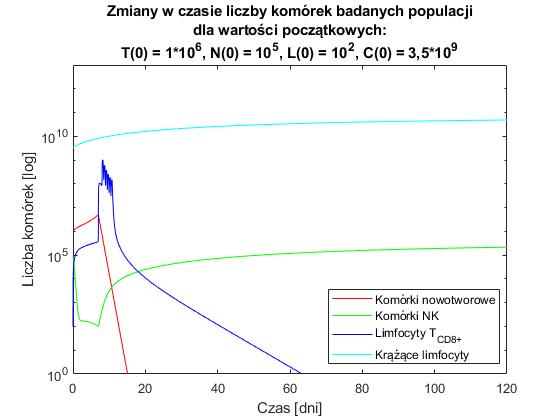
\includegraphics[width=0.45\textwidth]{wykres_immuno_zmiany_wielkosci_guza1e6}}
\quad
\subfloat[Zmiany w~czasie liczby kom�rek badanych populacji dla~pocz�tkowej liczby kom�rek nowotworowych $T(0) = 1,8 \cdot 10^{7}$. Widoczna (linia czerwona) stabilizacja liczby kom�rek nowotworowych po~28 dniach oko�o warto�ci $9,8 \cdot 10^{8}$.]{\label{wykres_immuno_zmiany_wielkosci_guza18e7}
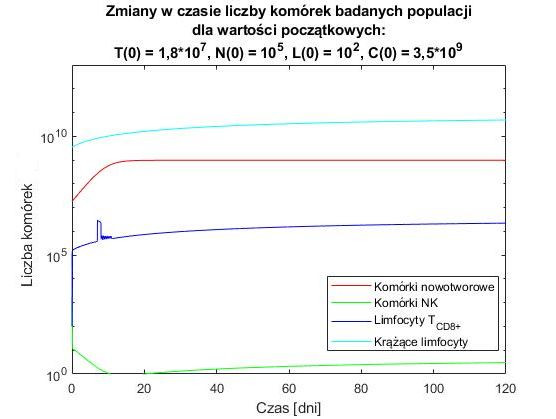
\includegraphics[width=0.45\textwidth]{wykres_immuno_zmiany_wielkosci_guza18e7}}
\quad
\subfloat[Zmiany w~czasie st�enia, dozowanych podczas immunoterapii, IL-2 dla~pocz�tkowej liczby kom�rek nowotworowych $T(0) = 10^{6}$ oraz~$T(0) = 1,8 \cdot 10^{7}$.]{\label{stezenie_immuno_zmiany_wielkosci_guza1e6}
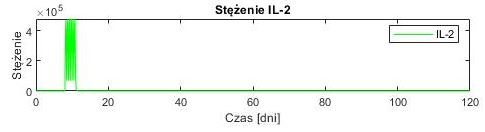
\includegraphics[width=0.45\textwidth]{stezenie_immuno_zmiany_wielkosci_guza1e6}}
\quad
\subfloat{\label{stezenie_immuno_zmiany_wielkosci_guza18e7}

\includegraphics[width=0.45\textwidth]{pustkja}}
\caption[Zmiany w~czasie liczby kom�rek badanych populacji oraz~st�enia IL-2 - immunoterapia, scenariusz I, zmiana wielko�ci guza w~dniu rozpocz�cia immunoterapii]{Zmiany w~czasie liczby kom�rek badanych populacji oraz~st�enia dozowanych podczas immunoterapii IL-2 dla~pocz�tkowej liczby kom�rek nowotworowych $T(0) = 10^{6}$ oraz~$T(0) = 1,8 \cdot 10^{7}$. Pocz�tkowa liczba kom�rek NK $N(0) = 10^{5}$, pocz�tkowa liczba limfocyt�w $T_{CD8+}$ $L(0) = 10^{2}$, pocz�tkowa liczba limfocyt�w kr���cych $C(0) = 3,5 \cdot 10^{9}$.}
\label{wykresy_immuno_zmiany_wielkosci_guza}
\end{figure}

\newpage
\textbf{Wnioski:}
\begin{itemize}
\item os�abiony uk�ad immunologiczny, reprezentowany poprzez liczb� kom�rek wyst�puj�cych naturalnie w~organizmie: kom�rek NK $N(0) = 10^{5}$, limfocyt�w $T_{CD8+}$ $L(0) = 10^{2}$ oraz~limfocyt�w kr���cych $C(0) = 3,5 \cdot 10^{9}$, wspomagany leczeniem metod� immunoterapii jest w~stanie zniszczy� kom�rki nowotworowe, je�li~ich~pocz�tkowa liczba $T(0) = 1 \cdot 10^{6}$ kom�rek, tzn. pocz�tkowa d�ugo�� promienia nowotworu to $R_{0} = 1,63$ mm (wielko��, przy kt�rej guz jest wykrywalny klinicznie), co~nie by�o mo�liwe w~przypadku braku leczenia;
\item leczenie metod� immunoterapii, zgodne z~warunkami pocz�tkowymi (Tab. \ref{warunki_pocz�tkowe_immunoterapii}) nie~jest skuteczne (nie nast�puje regresja nowotworu) dla~pocz�tkowej liczby kom�rek nowotworowych $T(0) = 1,8 \cdot 10^{7}$.
\end{itemize}

Immunoterapia to~metoda leczenia mniej szkodliwa ni�~chemioterapia, poniewa� skupia si� na~wzmocnieniu organizmu. Daje ona mo�liwo�� zniszczenia kom�rek nowotworowych, jednak tylko w~przypadku guza o~niewielkim rozmiarze lub wtedy, gdy~uk�ad immunologiczny jest zdrowy, nieos�abiony.

\newpage
\section{Scenariusz II -- zmiana dawki IL-2 $V_I$}
\noindent \textbf{Podejmowany problem:} \newline Wp�yw zmian dawki IL-2 $V_I$ na~skuteczno�� terapii.

\noindent \newline \textbf{Warunki pocz�tkowe:} 
\begin{itemize}
\item dla~pocz�tkowej wielko�ci badanych populacji, tj. pocz�tkow� liczb� kom�rek nowotworu $T(0)$, liczb� kom�rek NK $N(0)$, liczb� limfocyt�w $T_{CD8+}$ oraz~liczb� limfocyt�w kr���cych $C(0)$ przedstawia Tab. \ref{warunki_poczatkowe_z1};
\item dla~immunoterapii, tj. d�ugo�� cyklu, czas dozowania, schemat cyklu, dawk� dozowanych lek�w (IL-2 i TIL), liczb� powt�rze� cyklu oraz~dzie� rozpocz�cia immunoterapii przedstawia Tab. \ref{warunki_pocz�tkowe_immunoterapii}.
\end{itemize}

\noindent \newline \textbf{Przyj�te parametry:} \newline Parametry dla~modelu uwzgl�dniaj�cego leczenie przedstawia Tab. \ref{parametry_modelu_bez1} i~\ref{parametry_modelu_z1}.

\noindent \newline \textbf{Czas symulacji:} \newline Czas symulacji wynosi� $T_{k}$ = 120 dni. 

\noindent \newline \textbf{Wyniki symulacji:} \newline Wyniki przeprowadzonych symulacji dla~zmieniaj�cej si� dawki IL-2 $V_I$ dla~leczenia z~wykorzystaniem TIL oraz~bez wykorzystania TIL zebrano w~Tab. \ref{zmiany_dawki_IL2_przy_TIL}. \newline

Tab. \ref{zmiany_dawki_IL2_przy_TIL} przedstawia zmian� dawki IL-2 $V_I$. Dodatkowo, w~Tab. \ref{zmiany_dawki_IL2_przy_TIL} umieszczono dzie� regresji nowotworu oraz~liczb� kom�rek nowotworu T(120) w~ostatnim (120) dniu symulacji, a~tak�e~szacowan� obj�to�� i~d�ugo�� promienia nowotworu w~ostatnim (120) dniu symulacji (tj. w~chwili $T_{k}$ = 120 dni). Analiz� przeprowadzono dla~leczenia z~wykorzystaniem oraz~bez wykorzystania TIL.

\newpage
\begin{table}[h!]
\small
	\centering
	\caption[Wyniki symulacji - immunoterapia, scenariusz II, zmiana dawki IL-2 $V_I$]{Dawka IL-2 $V_I$, dzie� regresji nowotworu, liczba kom�rek nowotworowych T(120) w~ostatnim (120) dniu symulacji oraz~szacowana obj�to�� i~d�ugo�� promienia nowotworu w~ostatnim (120) dniu symulacji (tj. w~chwili $T_{k}$ = 120 dni) dla~leczenia z~wykorzystaniem oraz~bez wykorzystania TIL.}
\label{zmiany_dawki_IL2_przy_TIL}
\begin{tabular}{|c|c|c|c|c|} \hline \hline
        \multicolumn{5}{|c|}{Leczenie z~wykorzystaniem TIL} \\ \hline \hline
		Dawka & Dzie� regresji & $T(120)$ & Obj�to�� & D�ugo�� promienia \\
		IL-2 $V_I$ $[\dfrac{IU}{kg}]$ & nowotworu & $[liczba$ $kom$�$rek]$ & nowotworu [$mm^{3}$] & nowotworu [$mm$] \\ \hline
		$5 \cdot 10^{6}$ & brak & $9,8 \cdot 10^{8}$ & $980$ & $6,16$ \\ \hline
		$1 \cdot 10^{7}$ & brak & $9,8 \cdot 10^{8}$ & $980$ & $6,16$ \\ \hline
		$2 \cdot 10^{7}$ & 18,54 & $7,69 \cdot 10^{-85}$ & $7,69 \cdot 10^{-91}$ & $5,7 \cdot 10^{-31}$ \\ \hline
		$3 \cdot 10^{7}$ & 18,42 & $5,69 \cdot 10^{-85}$ & $5,69 \cdot 10^{-91}$ & $5,1 \cdot 10^{-31}$ \\ \hline
		$4 \cdot 10^{7}$ & 18,38 & $5,43 \cdot 10^{-85}$ & $5,43 \cdot 10^{-91}$ & $5,1 \cdot 10^{-31}$ \\ \hline
		$6 \cdot 10^{7}$ & 18,34 & $5,22 \cdot 10^{-85}$ & $5,22 \cdot 10^{-91}$ & $5 \cdot 10^{-31}$ \\ \hline
		$1 \cdot 10^{8}$ & 18,34 & $5,05 \cdot 10^{-85}$ & $5,05 \cdot 10^{-91}$ & $4,9 \cdot 10^{-31}$ \\ \hline \hline
		\multicolumn{5}{|c|}{Leczenie bez wykorzystania TIL} \\ \hline \hline
		Dawka & Dzie� regresji & $T(120)$ & Obj�to�� & D�ugo�� promienia \\
		IL-2 $V_I$ $[\dfrac{IU}{kg}]$ & nowotworu & $[liczba$ $kom$�$rek]$ & nowotworu [$mm^{3}$] & nowotworu [$mm$] \\ \hline
		$5 \cdot 10^{6}$ & brak & $9,8 \cdot 10^{8}$ & $980$ & $6,16$ \\ \hline
		$1 \cdot 10^{7}$ & brak & $9,8 \cdot 10^{8}$ & $980$ & $6,16$ \\ \hline
		$2 \cdot 10^{7}$ & 18,54 & $7,34 \cdot 10^{-85}$ & $7,34 \cdot 10^{-91}$ & $5,6 \cdot 10^{-31}$ \\ \hline
		$3 \cdot 10^{7}$ & 18,42 & $5,7 \cdot 10^{-85}$ & $5,7 \cdot 10^{-91}$ & $5,2 \cdot 10^{-31}$ \\ \hline
		$4 \cdot 10^{7}$ & 18,38 & $5,44 \cdot 10^{-85}$ & $5,44 \cdot 10^{-91}$ & $5,1 \cdot 10^{-31}$ \\ \hline
		$6 \cdot 10^{7}$ & 18,34 & $5,22 \cdot 10^{-85}$ & $5,22 \cdot 10^{-91}$ & $5 \cdot 10^{-31}$ \\ \hline
		$1 \cdot 10^{8}$ & 18,34 & $5,06 \cdot 10^{-85}$ & $5,06 \cdot 10^{-91}$ & $5 \cdot 10^{-31}$ \\ \hline
		\end{tabular}
\end{table} 

Przyk�adowo, Rys. \ref{wykresy_zmiany_dawki_IL2_przy_TIL} obrazuje zmiany w~czasie liczby kom�rek badanych populacji, tj. kom�rek nowotworowych, kom�rek NK, limfocyt�w $T_{CD8+}$ oraz~limfocyt�w kr���cych dla~immunoterapii z~wykorzystaniem IL-2 o~dawce $V_I = 2 \cdot 10^{7}$ $\dfrac{IU}{kg}$ oraz~TIL o~dawce $V_L = 10^{9}$ kom�rek (Rys. \ref{wykres_zmiany_dawki_IL2_przy_TIL}), a~tak�e zmiany w~czasie st�enia, dozowanych podczas immunoterapii, IL-2 (Rys. \ref{stezenie_zmiany_dawki_IL2_przy_TIL}). 

Symulacja zak�ada�a sze�ciokrotne powt�rzenie cyklu dozowania IL-2 oraz~jednokrotny cykl podawania TIL. Czas dawkowania IL-2 wynosi� 7 godzin i~12 minut. Czas dawkowania TIL wynosi� 1 dzie� (24 godziny). D�ugo�� przerwy pomi�dzy kolejnymi powt�rzeniami cyklu IL-2 wynosi�a 4 godziny i~48 minut. Dzie� rozpocz�cia dozowania IL-2 to~9 dzie� symulacji, natomiast rozpocz�cie dozowania TIL nast�pi�o w~8 dniu symulacji. 

\newpage
Dzi�ki zwi�kszeniu dawki IL-2 do~warto�ci $V_I = 2 \cdot 10^{7}$ $\dfrac{IU}{kg}$ immunoterapia by�a skuteczna w~przypadku guza o~pocz�tkowej liczbie kom�rek nowotworowych $T(0) = 1,8 \cdot 10^{7}$, czego nie~uda�o si� uzyska� w~symulacji \ref{immuno_zmiana_pocz_war_guza}. Regresja nast�pi�a po~19 dniach od~rozpocz�cia symulacji. Mo�na by�o zaobserwowa� znaczny wzrost liczby limfocyt�w $T_{CD8+}$ na~skutek zwi�kszenia dawki IL-2 $V_I$ (Rys. \ref{wykres_zmiany_dawki_IL2_przy_TIL}).

\begin{figure}[h!]
\centering
\subfloat[Zmiany w~czasie liczby kom�rek badanych populacji dla~dawki IL-2 $V_I = 2 \cdot 10^{7}$ $\dfrac{IU}{kg}$ dla~leczenia z~wykorzystaniem TIL. Widoczna (linia czerwona) regresja nowotworu po~19 dniach.]{\label{wykres_zmiany_dawki_IL2_przy_TIL}
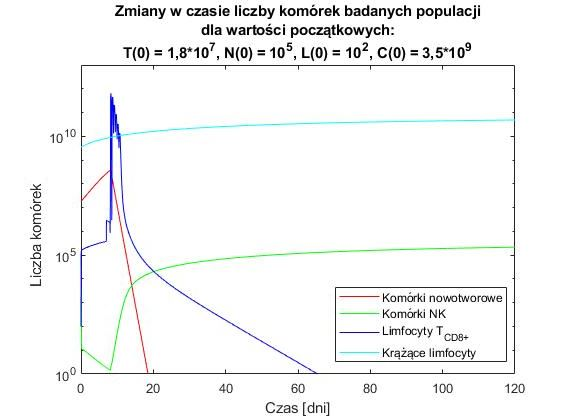
\includegraphics[width=0.5\textwidth]{wykres_zmiany_dawki_IL2_przy_TIL}}
\quad
\subfloat[Zmiany w~czasie st�enia, dozowanych podczas immunoterapii, IL-2 dla~dawki IL-2 $V_I = 2 \cdot 10^{7}$ $\dfrac{IU}{kg}$ dla~leczenia z~wykorzystaniem TIL.]{\label{stezenie_zmiany_dawki_IL2_przy_TIL}
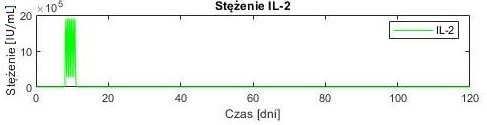
\includegraphics[width=0.5\textwidth]{stezenie_zmiany_dawki_IL2_przy_TIL}}
\caption[Zmiany w~czasie liczby kom�rek badanych populacji oraz~st�enia IL-2 - immunoterapia, scenariusz II, zmiana dawki IL-2 $V_I$]{Zmiany w~czasie liczby kom�rek badanych populacji oraz~st�enia dozowanych podczas immunoterapii IL-2 dla~dawki IL-2 $V_I = 2 \cdot 10^{7}$ $\dfrac{IU}{kg}$ dla~leczenia z~wykorzystaniem TIL. Pocz�tkowa liczba kom�rek nowotworowych $T(0) = 1,8 \cdot 10^{7}$, pocz�tkowa liczba kom�rek NK $N(0) = 10^{5}$, pocz�tkowa liczba limfocyt�w $T_{CD8+}$ $L(0) = 10^{2}$, pocz�tkowa liczba limfocyt�w kr���cych $C(0) = 3,5 \cdot 10^{9}$.}
\label{wykresy_zmiany_dawki_IL2_przy_TIL}
\end{figure}

\newpage
Cz�� wynik�w symulacji w~formie graficznej, przedstawia Rys. \ref{slupki_8.3}.

\begin{figure}[h!]
\centering
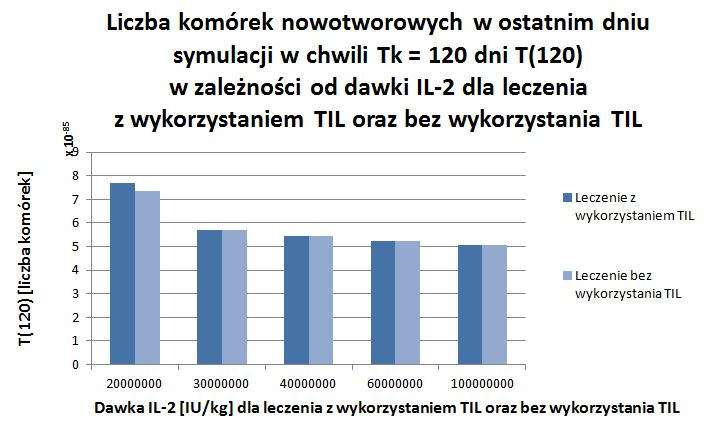
\includegraphics[width=0.8\textwidth]{slupki_8.3}
\caption{Liczba kom�rek nowotworowych $T(120)$ w ostatnim dniu symulacji w chwili $T_{k} = 120$ dni w zale�no�ci od dawki IL-2 $V_I$.}\label{slupki_8.3}
\end{figure}

\textbf{Wnioski:}
\begin{itemize}
\item zmiana dawki IL-2 $V_I$ ma~wp�yw na~skuteczno�� immunoterapii (wyst�pienie regresji nowotworu lub jej brak); zar�wno w~przypadku wykorzystania w~leczeniu IL-2 wraz z~TIL, jak~i~wy��cznie IL-2 dawk� konieczn� do~zniszczenia nowotworu (regresji) jest $V_I = 2 \cdot 10^{7}$ $\dfrac{IU}{kg}$;
\item zwi�kszanie dawki IL-2 $V_I$ (dla $V_I > 2 \cdot 10^{7}$ $\dfrac{IU}{kg}$) nie~ma~znacz�cego wp�ywu na~moment wyst�pienia regresji; w~ka�dym przypadku jest to~19 dzie� symulacji;
\item leczenie z~wykorzystaniem IL-2 oraz~TIL nie~r�ni si� znacz�co od~leczenia z~wykorzystaniem wy��cznie IL-2; wykorzystanie TIL w~leczeniu nie~ma~wp�ywu na~dzie� regresji nowotworu, jedyn� zmian� w~stosunku do~leczenia przy u�yciu wy��cznie IL-2 s�~bardzo ma�e zmiany liczby kom�rek nowotworowych T(120) w~ostatnim (120) dniu symulacji;
\item symulacja leczenia z~wykorzystaniem wy��cznie IL-2 wykaza�a, �e~leczenie to~jest w~stanie doprowadzi� do~regresji nowotworu, co~mo�e sugerowa�, �e~wykorzystanie TIL w~immunoterapii nie~jest konieczne.
\end{itemize}

Zgodnie z~przeprowadzon� analiz�, dawka IL-2 $V_I$ w~leczeniu metod� immunoterapii ma~wp�yw na~wyst�pienie regresji nowotworu, jednak jej zwi�kszanie nie~wp�ywa na~moment, w~kt�rym regresja ta~nast�puje. Wykazano tak�e, �e do~skuteczno�ci leczenia w~tym przypadku nie~jest konieczne u�ycie TIL.

\newpage
\section{Scenariusz III -- zmiana dawki TIL $V_L$}
\noindent \textbf{Podejmowany problem:} \newline Wp�yw zmian dawki TIL $V_L$ na~skuteczno�� terapii.

\noindent \newline \textbf{Warunki pocz�tkowe:} 
\begin{itemize}
\item dla~pocz�tkowej wielko�ci badanych populacji, tj. pocz�tkow� liczb� kom�rek nowotworu $T(0)$, liczb� kom�rek NK $N(0)$, liczb� limfocyt�w $T_{CD8+}$ oraz~liczb� limfocyt�w kr���cych $C(0)$ przedstawia Tab. \ref{warunki_poczatkowe_z1};
\item dla~immunoterapii, tj. d�ugo�� cyklu, czas dozowania, schemat cyklu, dawk� dozowanych lek�w (IL-2 i TIL), liczb� powt�rze� cyklu oraz~dzie� rozpocz�cia immunoterapii przedstawia Tab. \ref{warunki_pocz�tkowe_immunoterapii}.
\end{itemize}

\noindent \newline \textbf{Przyj�te parametry:} \newline Parametry dla~modelu uwzgl�dniaj�cego leczenie przedstawia Tab. \ref{parametry_modelu_bez1} i~\ref{parametry_modelu_z1}.

\noindent \newline \textbf{Czas symulacji:} \newline Czas symulacji wynosi� $T_{k}$ = 120 dni. 

\noindent \newline \textbf{Wyniki symulacji:} \newline Wyniki przeprowadzonych symulacji dla~zmieniaj�cej si� dawki TIL $V_L$ dla~leczenia z~wykorzystaniem oraz~bez wykorzystania IL-2 zebrano w~Tab. \ref{zmiany_dawki_TIL_przy_IL2}. \newline

Tab. \ref{zmiany_dawki_TIL_przy_IL2} przedstawia zmian� dawki TIL $V_L$. Dodatkowo, Tab. \ref{zmiany_dawki_TIL_przy_IL2} przedstawia dzie� regresji nowotworu oraz~liczb� kom�rek nowotworu T(120) w~ostatnim (120) dniu symulacji, a~tak�e~szacowan� obj�to�� i~d�ugo�� promienia nowotworu w~ostatnim (120) dniu symulacji (tj. w~chwili $T_{k}$ = 120 dni). Analiz� przeprowadzono dla~leczenia z~wykorzystaniem oraz~bez wykorzystania IL-2.

\newpage
\begin{table}[h!]
	\centering
	\caption[Wyniki symulacji - immunoterapia, scenariusz III, zmiana dawki TIL $V_L$]{Dawka TIL $V_L$, dzie� regresji nowotworu, liczba kom�rek nowotworowych w~ostatnim (120) dniu symulacji oraz~szacowana obj�to�� i~d�ugo�� promienia nowotworu w~ostatnim (120) dniu symulacji (tj. w~chwili $T_{k}$ = 120 dni) dla~leczenia z~wykorzystaniem oraz~bez wykorzystania IL-2.}
\label{zmiany_dawki_TIL_przy_IL2}
\begin{tabular}{|c|c|c|c|c|} \hline \hline
        \multicolumn{5}{|c|}{Leczenie z~wykorzystaniem IL-2} \\ \hline \hline
		Dawka TIL $V_L$ & Dzie� & $T(120)$ & Obj�to�� & D�ugo�� promienia \\
		$[liczba$ & regresji & $[liczba$ & nowotworu [$mm^{3}$] & nowotworu [$mm$] \\ 	
		$kom$�$rek]$ & nowotworu & $kom$�$rek]$ & & \\ \hline
		$1 \cdot 10^{9}$ & brak & $9,8 \cdot 10^{8}$ & $980$ & $6,16$ \\ \hline
		$1 \cdot 10^{10}$ & brak & $9,8 \cdot 10^{8}$ & $980$ & $6,16$ \\ \hline
		$2 \cdot 10^{10}$ & 17,79 & $1,86 \cdot 10^{-85}$ & $1,86 \cdot 10^{-91}$ & $3,5 \cdot 10^{-31}$ \\ \hline
		$5 \cdot 10^{10}$ & 17,21 & $6 \cdot 10^{-86}$ & $6 \cdot 10^{-92}$ & $2,4 \cdot 10^{-31}$ \\ \hline
		$1 \cdot 10^{11}$ & 17,17 & $5,53 \cdot 10^{-86}$ & $5,53 \cdot 10^{-92}$ & $2,4 \cdot 10^{-31}$ \\ \hline
		$1 \cdot 10^{15}$ & 17,17 & $5,38 \cdot 10^{-86}$ & $5,38 \cdot 10^{-92}$ & $2,3 \cdot 10^{-31}$ \\ \hline \hline
		\multicolumn{5}{|c|}{Leczenie bez wykorzystania IL-2} \\ \hline \hline
		Dawka TIL $V_L$ & Dzie� & $T(120)$ & Obj�to�� & D�ugo�� promienia \\
		$[liczba$ & regresji & $[liczba$ & nowotworu [$mm^{3}$] & nowotworu [$mm$] \\ 	
		$kom$�$rek]$ & nowotworu & $kom$�$rek]$ & & \\ \hline
		$1 \cdot 10^{9}$ & brak & $9,8 \cdot 10^{8}$ & $980$ & $6,16$ \\ \hline
		$1 \cdot 10^{10}$ & brak & $9,8 \cdot 10^{8}$ & $980$ & $6,16$ \\ \hline
		$1 \cdot 10^{11}$ & brak & $9,8 \cdot 10^{8}$ & $980$ & $6,16$ \\ \hline
		$1 \cdot 10^{15}$ & brak & $9,8 \cdot 10^{8}$ & $980$ & $6,16$ \\ \hline
		\end{tabular}
\end{table} 

Przyk�adowo, Rys. \ref{wykresy_zmiany_dawki_TIL_przy_IL2} obrazuje zmiany w~czasie liczby kom�rek badanych populacji, tj. kom�rek nowotworowych, kom�rek NK, limfocyt�w $T_{CD8+}$ oraz~limfocyt�w kr���cych dla~immunoterapii z~wykorzystaniem TIL o~dawce $V_L = 2 \cdot 10^{10}$ kom�rek oraz~IL-2 o~dawce $V_I = 5 \cdot 10^{6}$ $\dfrac{IU}{kg}$ (Rys. \ref{wykres_zmiany_dawki_TIL_przy_IL2}), a~tak�e zmiany w~czasie st�enia, dozowanego podczas immunoterapii, IL-2 (Rys. \ref{stezenie_zmiany_dawki_TIL_przy_IL2}). 

Symulacja zak�ada�a sze�ciokrotne powt�rzenie cyklu dozowania IL-2 oraz~jednokrotny cykl podawania TIL. Czas dawkowania IL-2 wynosi� 7 godzin i~12 minut. Czas dawkowania TIL wynosi� 1 dzie� (24 godziny). D�ugo�� przerwy pomi�dzy kolejnymi powt�rzeniami cyklu IL-2 wynosi�a 4 godziny i~48 minut. Dzie� rozpocz�cia dozowania IL-2 to~9 dzie� symulacji, natomiast rozpocz�cie dozowania TIL nast�pi�o w~8 dniu symulacji. 

\newpage
Dzi�ki zwi�kszeniu dawki TIL do~warto�ci $V_L = 2 \cdot 10^{10}$ kom�rek immunoterapia by�a skuteczna w~przypadku guza o~pocz�tkowej liczbie kom�rek nowotworowych $T(0) = 1,8 \cdot 10^{7}$, czego nie~uda�o si� uzyska� w~symulacji \ref{immuno_zmiana_pocz_war_guza}. Regresja nast�pi�a po~18 dniach od~rozpocz�cia symulacji. Mo�na by�o zaobserwowa� znaczny wzrost liczby limfocyt�w $T_{CD8+}$ na~skutek zwi�kszenia dawki TIL $V_L$ (Rys. \ref{wykres_zmiany_dawki_TIL_przy_IL2}).

\begin{figure}[h!]
\centering
\subfloat[Zmiany w~czasie liczby kom�rek badanych populacji dla~dawki TIL \\ $V_L = 2 \cdot 10^{10}$ kom�rek dla~leczenia z~wykorzystaniem IL-2. Widoczna (linia czerwona) regresja nowotworu po~18 dniach.]{\label{wykres_zmiany_dawki_TIL_przy_IL2}
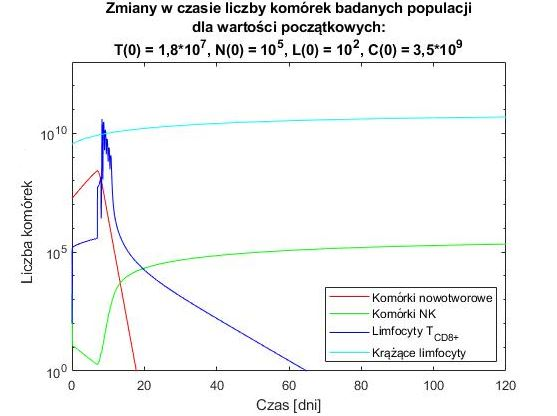
\includegraphics[width=0.5\textwidth]{wykres_zmiany_dawki_TIL_przy_IL2}}
\quad
\subfloat[Zmiany w~czasie st�enia, dozowanych podczas immunoterapii, IL-2 dla~dawki TIL \\ $V_L = 2 \cdot 10^{10}$ kom�rek dla~leczenia z~wykorzystaniem IL-2.]{\label{stezenie_zmiany_dawki_TIL_przy_IL2}
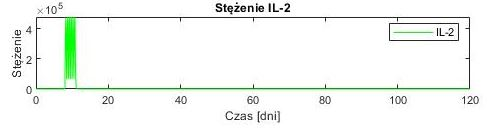
\includegraphics[width=0.5\textwidth]{stezenie_zmiany_dawki_TIL_przy_IL2}}
\caption[Zmiany w~czasie liczby kom�rek badanych populacji oraz~st�enia IL-2 - immunoterapia, scenariusz III, zmiana dawki TIL $V_L$]{Zmiany w~czasie liczby kom�rek badanych populacji oraz~st�enia dozowanych podczas immunoterapii IL-2 dla~dawki TIL $V_L = 2 \cdot 10^{10}$ kom�rek dla~leczenia z~wykorzystaniem IL-2. Pocz�tkowa liczba kom�rek nowotworowych $T(0) = 1,8 \cdot 10^{7}$, pocz�tkowa liczba kom�rek NK $N(0) = 10^{5}$, pocz�tkowa liczba limfocyt�w $T_{CD8+}$ $L(0) = 10^{2}$, pocz�tkowa liczba limfocyt�w kr���cych $C(0) = 3,5 \cdot 10^{9}$.}
\label{wykresy_zmiany_dawki_TIL_przy_IL2}
\end{figure}

\newpage
\textbf{Wnioski:}
\begin{itemize}
\item zmiana dawki TIL $V_L$ ma~wp�yw na~skuteczno�� immunoterapii (wyst�pienie regresji nowotworu lub jej brak) w~przypadku wykorzystania w~leczeniu zar�wno TIL oraz~IL-2; dawk� konieczn� do~regresji nowotworu jest $V_L = 2 \cdot 10^{10}$ kom�rek;
\item zwi�kszanie dawki TIL $V_L$ nie~ma~znacz�cego wp�ywu na~moment wyst�pienia regresji; w~ka�dym przypadku (dla $V_L \geq 2 \cdot 10^{10}$ kom�rek) jest to~18 dzie� symulacji;
\item leczenie z~wykorzystaniem TIL oraz~IL-2 r�ni si� znacz�co od~leczenia z~wykorzystaniem wy��cznie TIL; leczenie z~wykorzystaniem wy��cznie TIL nie~jest w~stanie doprowadzi� do~regresji nowotworu; wykorzystanie IL-2 w~immunoterapii dla~tego przypadku jest konieczne.
\end{itemize}

Zgodnie z~przeprowadzon� analiz�, dawka TIL $V_L$ w~leczeniu metod� immunoterapii (w po��czeniu z wykorzystaniem IL-2) ma~wp�yw na~skuteczno�� terapii (regresj� nowotworu), jednak nie ma znacz�cego wp�ywu na moment wyst�pienia regresji. Leczenie z wykorzystaniem wy��cznie TIL nie doprowadza w tym przypadku do regresji nowotworu.

\newpage
\section{Scenariusz IV -- zmiana liczby powt�rze� cyklu IL-2}
\noindent \textbf{Podejmowany problem:} \newline Wp�yw zmian liczby powt�rze� cyklu IL-2 na~skuteczno�� terapii.

\noindent \newline \textbf{Warunki pocz�tkowe:} 
\begin{itemize}
\item dla~pocz�tkowej wielko�ci badanych populacji, tj. pocz�tkow� liczb� kom�rek nowotworu $T(0)$, liczb� kom�rek NK $N(0)$, liczb� limfocyt�w $T_{CD8+}$ oraz~liczb� limfocyt�w kr���cych $C(0)$ przedstawia Tab. \ref{warunki_poczatkowe_z1};
\item dla~immunoterapii, tj. d�ugo�� cyklu, czas dozowania, schemat cyklu, dawk� dozowanych lek�w (IL-2 i TIL), liczb� powt�rze� cyklu oraz~dzie� rozpocz�cia immunoterapii przedstawia Tab. \ref{warunki_pocz�tkowe_immunoterapii}.
\end{itemize}

\noindent \newline \textbf{Przyj�te parametry:} \newline Parametry dla~modelu uwzgl�dniaj�cego leczenie przedstawia Tab. \ref{parametry_modelu_bez1} i~\ref{parametry_modelu_z1}.

\noindent \newline \textbf{Czas symulacji:} \newline Czas symulacji wynosi� $T_{k}$ = 120 dni. 

\noindent \newline \textbf{Wyniki symulacji:} \newline Wyniki przeprowadzonych symulacji dla~zmieniaj�cej si� liczby powt�rze� cyklu IL-2 \ref{zmiany_liczby_powtorzen_IL2}. \newline

Tab. \ref{zmiany_liczby_powtorzen_IL2} przedstawia zaminy liczby powt�rze� cyklu IL-2. Dodatkowo, zamieszczono w~Tab. \ref{zmiany_liczby_powtorzen_IL2} dzie� regresji nowotworu oraz~liczb� kom�rek nowotworu T(120) w~ostatnim (120) dniu symulacji, a~tak�e~szacowan� obj�to�� i~d�ugo�� promienia nowotworu w~ostatnim (120) dniu symulacji (tj. w~chwili $T_{k}$ = 120 dni). Analiz� przeprowadzono dla~pocz�tkowej liczby kom�rek nowotworowych r�wnej $T(0) = 1,8 \cdot 10^{7}$ oraz~$T(0) = 1 \cdot 10^{6}$.

\begin{table}[h!]
	\centering
	\caption[Wyniki symulacji - immunoterapia, scenariusz IV, zmiana liczby powt�rze� cyklu IL-2 dla~leczenia z~wykorzystaniem TIL]{Liczba powt�rze� cyklu IL-2, dzie� regresji nowotworu, liczba kom�rek nowotworowych T(120) w~ostatnim (120) dniu symulacji oraz~szacowana obj�to�� i~d�ugo�� promienia nowotworu w~ostatnim (120) dniu symulacji (tj. w~chwili $T_{k}$ = 120 dni) dla~pocz�tkowej liczby kom�rek nowotworowych r�wnej $T(0) = 1,8 \cdot 10^{7}$ oraz~$T(0) = 1 \cdot 10^{6}$.}
\label{zmiany_liczby_powtorzen_IL2}
\begin{tabular}{|c|c|c|c|c|} \hline \hline
        \multicolumn{5}{|c|}{Pocz�tkowa liczba kom�rek nowotworu $T(0) = 1,8 \cdot 10^{7}$} \\ \hline \hline
		Liczba & Dzie� & $T(120)$ & Obj�to�� & D�ugo�� \\
		powt�rze� & regresji & $[liczba$ & nowotworu & promienia \\
		cyklu IL-2 & nowotworu & $kom$�$rek]$ & [$mm^{3}$] & nowotworu [$mm$] \\ \hline
		6 & brak & $9,8 \cdot 10^{8}$ & $980$ & $6,16$ \\ \hline
		10 & brak & $9,8 \cdot 10^{8}$ & $980$ & $6,16$ \\ \hline
		14 & brak & $9,8 \cdot 10^{8}$ & $980$ & $6,16$ \\ \hline \hline
		\multicolumn{5}{|c|}{Pocz�tkowa liczba kom�rek nowotworu $T(0) =1 \cdot 10^{6}$} \\ \hline \hline
		Liczba & Dzie� & $T(120)$ & Obj�to�� & D�ugo�� \\
		powt�rze� & regresji & $[liczba$ & nowotworu & promienia \\
		cyklu IL-2 & nowotworu & $kom$�$rek]$ & [$mm^{3}$] & nowotworu [$mm$] \\ \hline
		6 & 15,13 & $1,07 \cdot 10^{-87}$ & $1,07 \cdot 10^{-93}$ & $6,4 \cdot 10^{-32}$ \\ \hline
		3 & 15,13 & $1,07 \cdot 10^{-87}$ & $1,07 \cdot 10^{-93}$ & $6,4 \cdot 10^{-32}$ \\ \hline
		1 & 15,13 & $1,07 \cdot 10^{-87}$ & $1,07 \cdot 10^{-93}$ & $6,4 \cdot 10^{-32}$ \\ \hline
		\end{tabular}
\end{table} 

\newpage 
Przyk�adowo, Rys. \ref{wykresy_zmiany_liczby_powtorzen_IL2} przedstawia zmiany w~czasie liczby kom�rek badanych populacji, tj. kom�rek nowotworowych, kom�rek NK, limfocyt�w $T_{CD8+}$ oraz~limfocyt�w kr���cych dla~immunoterapii z~wykorzystaniem IL-2 o~dawce $V_I = 5 \cdot 10^{6}$ $\dfrac{IU}{kg}$ i~liczbie powt�rze� cyklu r�wnej 14 oraz~jednokrotnym dozowaniem TIL o~dawce $V_L = 10^{9}$ kom�rek (Rys. \ref{wykres_zmiany_liczby_powtorzen_IL2}), a~tak�e zmiany w~czasie st�enia, dozowanych podczas immunoterapii, IL-2 (Rys. \ref{stezenie_zmiany_liczby_powtorzen_IL2}). 

Czas dawkowania IL-2 wynosi� 7 godzin i~12 minut. Czas dawkowania TIL wynosi� 1 dzie� (24 godziny). D�ugo�� przerwy pomi�dzy kolejnymi powt�rzeniami cyklu IL-2 wynosi�a 4 godziny i~48 minut. Dzie� rozpocz�cia dozowania IL-2 to~9 dzie� symulacji, natomiast rozpocz�cie dozowania TIL nast�pi�o w~8 dniu symulacji. 

\newpage
Mimo wielokrotnego powtarzania cyklu IL-2, regresja nie~nast�pi�a, a~liczba kom�rek nowotworowych ustabilizowa�a si� w~28 dniu symulacji (Rys. \ref{wykres_zmiany_liczby_powtorzen_IL2}). Mo�na by�o zaobserwowa� nag�y wzrost liczby limfocyt�w $T_{CD8+}$ na~skutek podania TIL oraz~nieznaczne zmiany liczby limfocyt�w $T_{CD8+}$ przy kolejnych powt�rzeniach cyklu IL-2.

\begin{figure}[h!]
\centering
\subfloat[Zmiany w~czasie liczby kom�rek badanych populacji dla~liczby powt�rze� cyklu IL-2 r�wnej 14. Widoczna (linia czerwona) stabilizacja liczby kom�rek nowotworowych po~28 dniach oko�o warto�ci $9,8 \cdot 10^{8}$. ]{\label{wykres_zmiany_liczby_powtorzen_IL2}
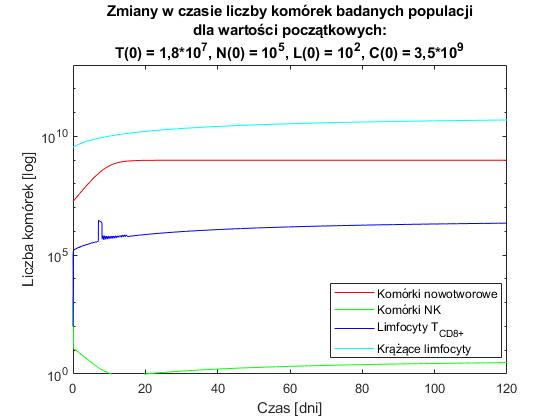
\includegraphics[width=0.5\textwidth]{wykres_zmiany_liczby_powtorzen_IL2}}
\quad
\subfloat[Zmiany w~czasie st�enia, dozowanych podczas immunoterapii, IL-2 dla~liczby powt�rze� cyklu IL-2 r�wnej 14.]{\label{stezenie_zmiany_liczby_powtorzen_IL2}
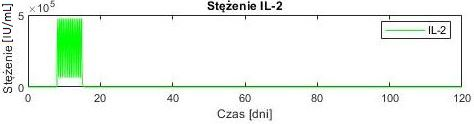
\includegraphics[width=0.5\textwidth]{stezenie_zmiany_liczby_powtorzen_IL2}}
\caption[Zmiany w~czasie liczby kom�rek badanych populacji oraz~st�enia IL-2 - immunoterapia, scenariusz IV, zmiana liczby powt�rze� cyklu IL-2 dla~leczenia z~wykorzystaniem TIL]{Zmiany w~czasie liczby kom�rek badanych populacji oraz~st�enia dozowanego podczas immunoterapii IL-2 dla~liczby powt�rze� cyklu IL-2 r�wnej 14. Pocz�tkowa liczba kom�rek nowotworowych $T(0) = 1,8 \cdot 10^{7}$, pocz�tkowa liczba kom�rek NK $N(0) = 10^{5}$, pocz�tkowa liczba limfocyt�w $T_{CD8+}$ $L(0) = 10^{2}$, pocz�tkowa liczba limfocyt�w kr���cych $C(0) = 3,5 \cdot 10^{9}$.}
\label{wykresy_zmiany_liczby_powtorzen_IL2}
\end{figure}

\textbf{Wnioski:}
\begin{itemize}
\item liczba powt�rze� cyklu IL-2 nie~ma~wp�ywu na~skuteczno�� leczenia (wyst�pienie regresji nowotworu); niezale�nie od~liczby powt�rze� cyklu (analizowano: 6, 10 oraz~14 powt�rze�) nie~wyst�puje regresja guza dla~pocz�tkowej liczby kom�rek nowotworowych $T(0) = 1,8 \cdot 10^{7}$; 
\item dla~ma�ej pocz�tkowej liczby kom�rek nowotworowych $T(0) = 1 \cdot 10^{6}$ zmiana liczby powt�rze� cyklu IL-2 nie~wp�ywa na~skuteczno�� leczenia (w ka�dym przypadku nast�puje regresja nowotworu) ani~na moment wyst�pienia regresji (w ka�dym przypadku dniem regresji jest 16 dzie� symulacji).
\end{itemize}

W przeciwie�stwie do~leczenia metod� chemioterapii, liczba powt�rze� cyklu leczenia (dozowania IL-2) w~immunoterapii nie~ma~wp�ywu na~efekt terapii, a~regresja guza nie~wyst�puje dla~guza o~du�ej pocz�tkowej liczbie kom�rek nowotworowych ($T(0) = 1,8 \cdot 10^{7}$). Dla mniejszych guz�w ($T(0) = 1 \cdot 10^{6}$) liczba powt�rze� cyklu r�wnie�~nie~wp�ywa na~efekt terapii (w ka�dym przypadku regresja wyst�puje), wi�c immunoterapi� mo�na ograniczy� do~jednego cyklu dozowania IL-2.

\newpage
\section{Scenariusz V -- zmiana dnia rozpocz�cia immunoterapii}
\noindent \textbf{Podejmowany problem:} \newline Wp�yw zmian dnia rozpocz�cia immunoterapii (dozowania IL-2 lub TIL) na~skuteczno�� terapii.

\noindent \newline \textbf{Warunki pocz�tkowe:} 
\begin{itemize}
\item dla~pocz�tkowej wielko�ci badanych populacji, tj. pocz�tkow� liczb� kom�rek nowotworu $T(0)$, liczb� kom�rek NK $N(0)$, liczb� limfocyt�w $T_{CD8+}$ oraz~liczb� limfocyt�w kr���cych $C(0)$ przedstawia Tab. \ref{warunki_poczatkowe_z1};
\item dla~immunoterapii, tj. d�ugo�� cyklu, czas dozowania, schemat cyklu, dawk� dozowanych lek�w (IL-2 i TIL), liczb� powt�rze� cyklu oraz~dzie� rozpocz�cia immunoterapii przedstawia Tab. \ref{warunki_pocz�tkowe_immunoterapii}.
\end{itemize}

\noindent \newline \textbf{Przyj�te parametry:} \newline Parametry dla~modelu uwzgl�dniaj�cego leczenie przedstawia Tab. \ref{parametry_modelu_bez1} i~\ref{parametry_modelu_z1}.

\noindent \newline \textbf{Czas symulacji:} \newline Czas symulacji wynosi� $T_{k}$ = 120 dni. 

\noindent \newline \textbf{Wyniki symulacji:} \newline Wyniki przeprowadzonych symulacji dla~zmieniaj�cego si� dnia rozpocz�cia immunoterapii zebrano w~Tab. \ref{zmiany_dnia_rozpoczecia_immunoterapii_IL2}. \newline

Tab. \ref{zmiany_dnia_rozpoczecia_immunoterapii_IL2} przedstawia zmiany dnia rozpocz�cia immunoterapii. Dodatkowo, w~Tab. \ref{zmiany_dnia_rozpoczecia_immunoterapii_IL2} zamieszczono dzie� regresji nowotworu oraz~liczb� kom�rek nowotworu T(120) w~ostatnim (120) dniu symulacji, a~tak�e~szacowan� obj�to�� i~d�ugo�� promienia nowotworu w~ostatnim (120) dniu symulacji (tj. w~chwili $T_{k}$ = 120 dni). Analiz� przeprowadzono dla~zmieniaj�cego si� dnia rozpocz�cia dozowania IL-2 oraz~TIL.

\begin{table}[h!]
	\centering
	\caption[Wyniki symulacji - immunoterapia, scenariusz V, zmiana dnia rozpocz�cia immunoterapii (dozowania IL-2 lub TIL)]{Dzie� rozpocz�cia immunoterapii, dzie� regresji nowotworu, liczba kom�rek nowotworowych T(120) w~ostatnim (120) dniu symulacji oraz~szacowana obj�to�� i~d�ugo�� promienia nowotworu w~ostatnim (120) dniu symulacji (tj. w~chwili $T_{k}$ = 120 dni) dla~IL-2 (przy dozowaniu TIL zgodnie z~warunkami pocz�tkowymi (\ref{warunki_pocz�tkowe_immunoterapii})) oraz~dla~TIL (przy dozowaniu IL-2 zgodnie z~warunkami pocz�tkowymi (\ref{warunki_pocz�tkowe_immunoterapii})).}
\label{zmiany_dnia_rozpoczecia_immunoterapii_IL2}
\begin{tabular}{|c|c|c|c|c|} \hline \hline
        \multicolumn{5}{|c|}{IL-2} \\ \hline \hline
		Dzie� & Dzie� & $T(120)$ & Obj�to�� & D�ugo�� promienia \\
		rozpocz�cia & regresji & $[liczba$ $kom$�$rek]$ & nowotworu & nowotworu \\
		immunoterapii & nowotworu & & [$mm^{3}$] & [$mm$] \\ \hline
		9 & brak & $9,8 \cdot 10^{8}$ & $980$ & $6,16$ \\ \hline
		6 & brak & $9,8 \cdot 10^{8}$ & $980$ & $6,16$ \\ \hline
		5 & 13,84 & $9,46 \cdot 10^{-89}$ & $9,46 \cdot 10^{-95}$ & $2,8 \cdot 10^{-32}$ \\ \hline
		4 & 12,58 & $8,3 \cdot 10^{-90}$ & $8,3 \cdot 10^{-96}$ & $1,3 \cdot 10^{-32}$ \\ \hline
		3 & 11,34 & $7,76 \cdot 10^{-92}$ & $7,76 \cdot 10^{-98}$ & $2,7 \cdot 10^{-33}$ \\ \hline
		2 & 10,08 & $7,38 \cdot 10^{-92}$ & $7,38 \cdot 10^{-98}$ & $2,6 \cdot 10^{-33}$ \\ \hline
		1 & 8,88 & $7,17 \cdot 10^{-93}$ & $7,17 \cdot 10^{-99}$ & $1,2 \cdot 10^{-33}$ \\ \hline \hline
		 \multicolumn{5}{|c|}{TIL} \\ \hline \hline
		Dzie� & Dzie� & $T(120)$ & Obj�to�� & D�ugo�� promienia \\
		rozpocz�cia & regresji & $[liczba$ $kom$�$rek]$ & nowotworu & nowotworu \\
		immunoterapii & nowotworu & & [$mm^{3}$] & [$mm$] \\ \hline
		9 & brak & $9,8 \cdot 10^{8}$ & $980$ & $6,16$ \\ \hline
		4 & brak & $9,8 \cdot 10^{8}$ & $980$ & $6,16$ \\ \hline
		3 & 12,29 & $4,95 \cdot 10^{-90}$ & $4,95 \cdot 10^{-96}$ & $1,1 \cdot 10^{-32}$ \\ \hline
		2 & 10,04 & $6,55 \cdot 10^{-92}$ & $6,55 \cdot 10^{-98}$ & $2,5 \cdot 10^{-33}$ \\ \hline
		1 & 8,8 & $6,26 \cdot 10^{-93}$ & $6,26 \cdot 10^{-99}$ & $1,1 \cdot 10^{-33}$ \\ \hline
		\end{tabular}
\end{table} 

\newpage 
Przyk�adowo, Rys. \ref{wykresy_zmiany_dnia_rozpoczecia_immunoterapii_IL2} ukazuje zmiany w~czasie liczby kom�rek badanych populacji, tj. kom�rek nowotworowych, kom�rek NK, limfocyt�w $T_{CD8+}$ oraz~limfocyt�w kr���cych dla~immunoterapii (dozowania IL-2) rozpocz�tej 5 dnia symulacji (Rys. \ref{wykres_zmiany_dnia_rozpoczecia_immunoterapii_IL2}), a~tak�e zmiany w~czasie st�enia, dozowanych podczas immunoterapii, IL-2 (Rys. \ref{stezenie_zmiany_dnia_rozpoczecia_immunoterapii_IL2}). 

Dawka IL-2 $V_I = 5 \cdot 10^{6}$ $\dfrac{IU}{kg}$, dawka TIL $V_L = 10^{9}$ kom�rek. Czas dawkowania IL-2 wynosi� 7 godzin i~12 minut. Czas dawkowania TIL wynosi� 1 dzie� (24 godziny). D�ugo�� przerwy pomi�dzy kolejnymi powt�rzeniami cyklu IL-2 wynosi�a 4 godziny i~48 minut. Rozpocz�cie dozowania TIL nast�pi�o w~8 dniu symulacji. Liczba powt�rze� cyklu IL-2 wynosi�a 6, natomiast dozowanie TIL by�o jednokrotne. 

\newpage
Wcze�niejsze rozpocz�cie (dzie� 5) dozowania IL-2 wywo�uje regresj� nowotworu w~14 dniu symulacji (\ref{wykres_zmiany_dnia_rozpoczecia_immunoterapii_IL2}).

\begin{figure}[h!]
\centering
\subfloat[Zmiany w~czasie liczby kom�rek badanych populacji dla~immunoterapii (dozowania IL-2) rozpocz�tej 5 dnia. Widoczna (linia czerwona) regresja nowotworu po~14 dniach.]{\label{wykres_zmiany_dnia_rozpoczecia_immunoterapii_IL2}
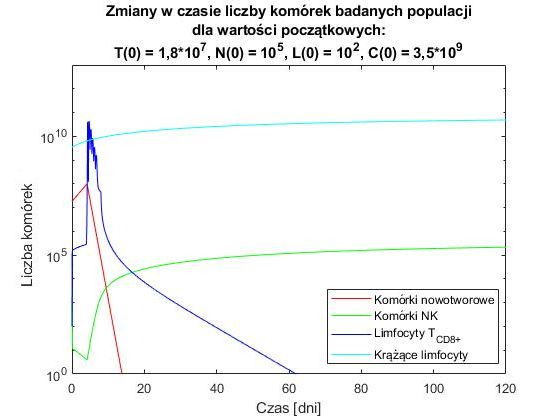
\includegraphics[width=0.5\textwidth]{wykres_zmiany_dnia_rozpoczecia_immunoterapii_IL2}}
\quad
\subfloat[Zmiany w~czasie st�enia, dozowanych podczas immunoterapii, IL-2 dla~immunoterapii (dozowania IL-2) rozpocz�tej 5 dnia.]{\label{stezenie_zmiany_dnia_rozpoczecia_immunoterapii_IL2}
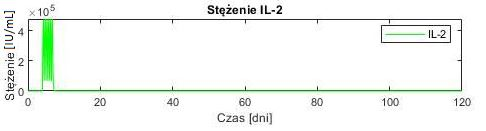
\includegraphics[width=0.5\textwidth]{stezenie_zmiany_dnia_rozpoczecia_immunoterapii_IL2}}
\caption[Zmiany w~czasie liczby kom�rek badanych populacji oraz~st�enia IL-2 - immunoterapia, scenariusz V, zmiana dnia rozpocz�cia immunoterapii (dozowania IL-2 lub TIL)]{Zmiany w~czasie liczby kom�rek badanych populacji oraz~st�enia dozowanego podczas immunoterapii IL-2 dla~immunoterapii (dozowania IL-2) rozpocz�tej 5 dnia. Pocz�tkowa liczba kom�rek nowotworowych $T(0) = 1,8 \cdot 10^{7}$, pocz�tkowa liczba kom�rek NK $N(0) = 10^{5}$, pocz�tkowa liczba limfocyt�w $T_{CD8+}$ $L(0) = 10^{2}$, pocz�tkowa liczba limfocyt�w kr���cych $C(0) = 3,5 \cdot 10^{9}$.}
\label{wykresy_zmiany_dnia_rozpoczecia_immunoterapii_IL2}
\end{figure}

\textbf{Wnioski:}
\begin{itemize}
\item dzie� rozpocz�cia immunoterapii (dozowania IL-2) przy dozowaniu TIL zgodnie z~warunkami pocz�tkowymi (Tab. \ref{warunki_pocz�tkowe_immunoterapii}) ma~wp�yw na~skuteczno�� leczenia (wyst�pienie regresji nowotworu lub jej brak); przy rozpocz�ciu dozowania IL-2 w~5 dniu symulacji (tj. 4 dni wcze�niej ni�~dla~warunk�w pocz�tkowych (Tab. \ref{warunki_pocz�tkowe_immunoterapii}), gdzie nie~nast�puje regresja) w~14 dniu symulacji wyst�puje regresja nowotworu;
\item dzie� rozpocz�cia immunoterapii (dozowania IL-2) przy dozowaniu TIL zgodnie z~warunkami pocz�tkowymi (Tab. \ref{warunki_pocz�tkowe_immunoterapii}) ma~wp�yw na~czas wyst�pienia regresji; od~dnia rozpocz�cia dozowania IL-2 do~dnia regresji mija 9 dni (z wyj�tkiem rozpocz�cia dozowania IL-2 w~pierwszym dniu - wtedy regresja nast�puje po~8 kolejnych dniach symulacji);
\item dzie� rozpocz�cia immunoterapii (dozowania TIL) przy dozowaniu IL-2 zgodnie z~warunkami pocz�tkowymi (Tab. \ref{warunki_pocz�tkowe_immunoterapii}) ma~wp�yw na~skuteczno�� leczenia (wyst�pienie regresji nowotworu lub jej brak); przy rozpocz�ciu dozowania TIL w~3 dniu symulacji (6 dni wcze�niej ni�~dla~warunk�w pocz�tkowych (Tab. \ref{warunki_pocz�tkowe_immunoterapii}), gdzie nie~nast�puje regresja) w~13 dniu symulacji wyst�puje regresja nowotworu;
\item dzie� rozpocz�cia immunoterapii (dozowania TIL) przy dozowaniu IL-2 zgodnie z~warunkami pocz�tkowymi (Tab. \ref{warunki_pocz�tkowe_immunoterapii}) ma~wp�yw na~czas wyst�pienia regresji; rozpocz�cie dozowania TIL o~1 dzie� wcze�niej skutkuje skr�ceniem czasu koniecznego do~wyst�pienia regresji o~1 dzie�, tj. dla~rozpocz�cia leczenia dnia: 3, 2 oraz~1 czas do~regresji wynosi, odpowiednio: 10, 9 oraz~8 dni.
\end{itemize}

Podobnie, jak~w~przypadku chemioterapii, skuteczno�� leczenia zale�y od~dnia jej~rozpocz�cia, a~przyspieszenie jej~o~zaledwie kilka dni mo�e decydowa� o~wyst�pieniu regresji nowotworu. R�wnocze�nie, dzie� rozpocz�cia immunoterapii nie~wp�ywa znacz�co na~czas od~momentu rozpocz�cia leczenia do~momentu wyst�pienia regresji.

\newpage
\chapter{Leczenie metodami skojarzonymi -- symulacje wykonane dla~modelu leczonego guza} \label{sym_ch_i}

W symulacji leczenia skojarzonymi metodami chemioterapii i~immunoterapii badano:
\begin{itemize}
\item zmiany warunk�w pocz�tkowych chemioterapii przy sta�ych warunkach pocz�tkowych immunoterapii,
\item zmiany warunk�w pocz�tkowych immunoterapii przy sta�ych warunkach pocz�tkowych chemioterapii,
\item zmiany warunk�w pocz�tkowych immunoterapii (dawki IL-2 $V_I$) w~celu uzyskania pozytywnego efektu leczenia dla~okre�lonych warunk�w pocz�tkowych chemioterapii;
\item zmiany kolejno�ci wdro�enia poszczeg�lnych terapii;
\item efekty leczenia u~r�nych pacjent�w w~oparciu o~ich~cechy osobnicze (reprezentuj�ce kondycj� ich uk�ad�w immunologicznych).
\end{itemize}

Przyk�adowo, Rys. \ref{wykresy_skojarzone} przedstawia zmiany w~czasie liczby kom�rek badanych populacji, tj. kom�rek nowotworowych, kom�rek NK, limfocyt�w $T_{CD8+}$ oraz~limfocyt�w kr���cych dla~leczenia skojarzonego metodami chemioterapii i~immunoterapii (Rys. \ref{wykres_skojarzone}), a~tak�e zmiany w~czasie st�enia, cytostatyka i~IL-2, dozowanych podczas leczenia skojarzonego (Rys. \ref{stezenie_skojarzone}). Przyj�to dawki: cytostatyka $V_M = 5$ $\dfrac{mg}{m^{2}}$, IL-2 $V_I = 5 \cdot 10^{6}$ $\dfrac{IU}{kg}$ oraz~TIL $V_L = 10^{9}$ kom�rek. Czas dawkowania cytostatyka oraz~TIL wynosi� 1 dzie� (24 godziny), a~IL-2 7 godzin i~12 minut. Liczba powt�rze� cyklu wynosi�a, odpowiednio: chemioterapii 9, IL-2 6, TIL 1. D�ugo�� przerwy pomi�dzy kolejnymi powt�rzeniami cyklu chemioterapii wynosi�a 3 dni, natomiast dla~IL-2 4 godziny i~48 minut. Dozowanie cytostatyka rozpocz�cto pierwszego dnia, TIL 8 dnia, a~IL-2 9 dnia symulacji. D�ugo�� cyklu chemioterapii by�a r�wna 8 dni. 

\newpage
Symulacja zak�ada�a po��czenie metod chemioterapii i~immunoterapii w~leczeniu nowotworu, kt�re dla~podanych warunk�w stosowane osobno by�y nieskuteczne. Takie skojarzenie chemioterapii i~immunoterapii skutkuje regresj� nowotworu w~15 dniu symulacji.

\begin{figure}[h!]
\centering
\subfloat[Zmiany w~czasie liczby kom�rek badanych populacji dla~leczenia z~wykorzystaniem skojarzonych metod chemioterapii i~immunoterapii (dla~warunk�w pocz�tkowych Tab. \ref{warunki pocz�tkowe_chemioterapii}, Tab. \ref{warunki_pocz�tkowe_immunoterapii} i~d�ugo�ci cyklu chemioterapii r�wnej 8 dni) z~widoczn� regresj� nowotworu po~15 dniach ($T_{r}$~$\approx$ 15 dni, tj. 360 godzin).]{\label{wykres_skojarzone}
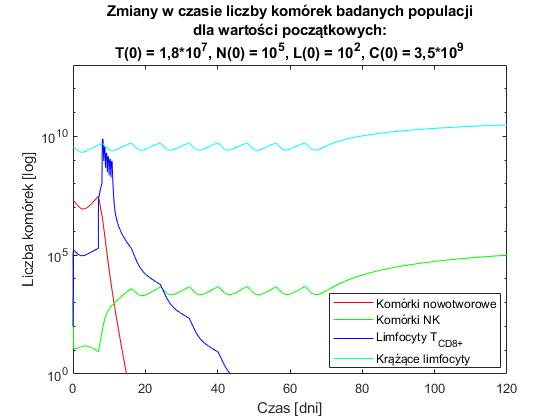
\includegraphics[width=0.45\textwidth]{wykres_skojarzone}}
\quad
\subfloat[Zmiany w~czasie st�enia, dozowanego podczas leczenia skojarzonego, cytostatyka oraz~IL-2.]{\label{stezenie_skojarzone}
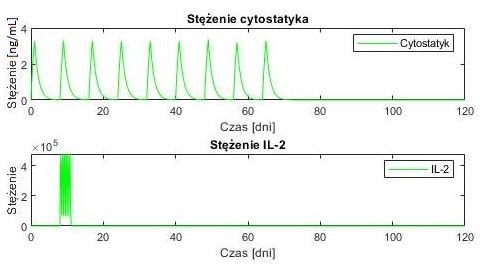
\includegraphics[width=0.45\textwidth]{stezenie_skojarzone}}
\caption[Zmiany w~czasie liczby kom�rek badanych populacji oraz~st�enia cytostatyka i~IL-2 - leczenie skojarzonymi metodami chemioterapii i~immunoterapii]{Zmiany w~czasie liczby kom�rek badanych populacji oraz~st�enia, dozowanego podczas leczenia skojarzonego cytostatyka oraz~IL-2 dla~warunk�w pocz�tkowych (Tab. \ref{warunki pocz�tkowe_chemioterapii}, Tab. \ref{warunki_pocz�tkowe_immunoterapii}) i~d�ugo�ci cyklu chemioterapii r�wnej 8 dni). Pocz�tkowa liczba kom�rek nowotworowych $T(0) = 1,8 \cdot 10^{7}$, pocz�tkowa liczba kom�rek NK $N(0) = 10^{5}$, pocz�tkowa liczba limfocyt�w $T_{CD8+}$ $L(0) = 10^{2}$, pocz�tkowa liczba limfocyt�w kr���cych $C(0) = 3,5 \cdot 10^{9}$.}
\label{wykresy_skojarzone}
\end{figure}

We~wszystkich symulacjach leczenia skojarzonymi metodami chemioterapii i~immunoterapii analizowano zmiany odpowiedzi uk�adu immunologicznego (tj. liczby kom�rek nowotworowych oraz~kom�rek uk�adu odporno�ciowego) po~120 dniach ($T_{k} = 120$ dni) symulacji w~zale�no�ci od~wy�ej wymienionych zmian okre�laj�cych biochemioterapi�.

\newpage
\section{Scenariusz I -- zmiana warunk�w pocz�tkowych chemioterapii} \label{ss1}

\noindent \textbf{Podejmowany problem:} \newline Zmiany warunk�w pocz�tkowych chemioterapii, tj. d�ugo�ci cyklu chemioterapii, dawki dozowanego cytostatyka $V_M$, liczby powt�rze� cyklu oraz~dnia rozpocz�cia chemioterapii przy~sta�ych warunkach pocz�tkowych immunoterapii.

\noindent \newline \textbf{Warunki pocz�tkowe:}
\begin{itemize}
\item dla~pocz�tkowej wielko�ci badanych populacji, tj. pocz�tkow� liczb� kom�rek nowotworu $T(0)$, liczb� kom�rek NK $N(0)$, liczb� limfocyt�w $T_{CD8+}$ oraz~liczb� limfocyt�w kr���cych $C(0)$ przedstawia Tab. \ref{warunki_poczatkowe_z1};
\item dla~chemioterapii, tj. d�ugo�� cyklu, czas dozowania cytostatyka, schemat cyklu, dawk� dozowanego cytostatyka $V_M$, liczb� powt�rze� cyklu oraz~dzie� rozpocz�cia chemioterapii przedstawia Tab. \ref{warunki pocz�tkowe_chemioterapii};
\item dla~immunoterapii, tj. d�ugo�� cyklu, czas dozowania, schemat cyklu, dawk� dozowanych lek�w (IL-2 i TIL), liczb� powt�rze� cyklu oraz~dzie� rozpocz�cia immunoterapii przedstawia Tab. \ref{warunki_pocz�tkowe_immunoterapii}.
\end{itemize}

\noindent \newline \textbf{Przyj�te parametry:} \newline Parametry dla~modelu uwzgl�dniaj�cego leczenie przedstawia Tab. \ref{parametry_modelu_bez1} i~\ref{parametry_modelu_z1}.

\noindent \newline \textbf{Czas symulacji:} \newline Czas symulacji wynosi� $T_{k}$ = 120 dni. 

\noindent \newline \textbf{Wyniki symulacji:} \newline Wyniki przeprowadzonych symulacji dla~zmieniaj�cych si� warunk�w pocz�tkowych chemioterapii przy sta�ej warto�ci warunk�w pocz�tkowych immunoterapii zebrano w~Tab. \ref{zmiana_cehmio_stale_immuno_dni_cyklu} - \ref{zmiana_cehmio_stale_immuno_dzien_rozpoczecia}.

\newpage

\subsection{Zmiana d�ugo�ci cyklu chemioterapii}

Tab. \ref{zmiana_cehmio_stale_immuno_dni_cyklu} przedstawia zmiany d�ugo�ci cyklu chemioterapii (przerw� pomi�dzy dozowaniem poszczeg�lnych dawek). Ponadto, tabela zawiera schemat cyklu (rozumiany jako [dozowanie leku [dni] przerwa [dni]), dzie� regresji nowotworu (rozumiany jako dzie�, w~kt�rym liczba kom�rek nowotworowych spada i~utrzymuje si� poni�ej warto�ci $T = 1$) oraz~liczb� kom�rek nowotworu T(120) w~ostatnim (120) dniu symulacji, a~tak�e~szacowan� obj�to�� i~d�ugo�� promienia nowotworu w~ostatnim (120) dniu symulacji (tj. w~chwili $T_{k}$ = 120 dni).

\begin{table}[h!]
	\centering
	\caption[Wyniki symulacji - leczenie skojarzonymi metodami chemioterapii i~immunoterapii, scenariusz I, zmiana d�ugo�ci cyklu]{D�ugo�� oraz~schemat cyklu chemioterapii, dzie� regresji nowotworu, liczba kom�rek nowotworowych T(120) w~ostatnim (120) dniu symulacji oraz~szacowana obj�to�� i~d�ugo�� promienia nowotworu w~ostatnim (120) dniu symulacji dla~immunoterapii o~warunkach pocz�tkowych (Tab. \ref{warunki_pocz�tkowe_immunoterapii}).}
\label{zmiana_cehmio_stale_immuno_dni_cyklu}
\begin{tabular}{|c|c|c|c|c|c|} \hline
       D�ugo�� & Schemat & Dzie� & $T(120)$ & Obj�to�� & D�ugo��  \\
		cyklu & cyklu & regresji & $[liczba$  & nowotworu & promienia  \\ 
		$[dni]$ & & nowotworu & $kom$�$rek]$ & [$mm^{3}$] & nowotworu [$mm$] \\ \hline
		4 & [1 3] & 13,25 & $9,43 \cdot 10^{-95}$ & $9,43 \cdot 10^{-101}$ & $2,8 \cdot 10^{-34}$ \\ \hline
		8 & [1 7] & 14,79 & $5,57 \cdot 10^{-95}$ & $5,57 \cdot 10^{-101}$ & $2,4 \cdot 10^{-34}$ \\ \hline
		20 & [1 19] & 16,08 & $8,92 \cdot 10^{-92}$ & $8,92 \cdot 10^{-98}$ & $2,8 \cdot 10^{-33}$ \\ \hline
		50 & [1 49] & 16,08 & $5,95 \cdot 10^{-89}$ & $5,95 \cdot 10^{-95}$ & $2,4 \cdot 10^{-32}$ \\ \hline
		100 & [1 99] & 16,08 & $6,47 \cdot 10^{-88}$ & $6,47 \cdot 10^{-94}$ & $5,4 \cdot 10^{-32}$ \\ \hline
		120 & [1 199] & 16,08 & $6,71 \cdot 10^{-87}$ & $6,71 \cdot 10^{-93}$ & $1,2 \cdot 10^{-31}$ \\ \hline
		\end{tabular}
\end{table} 

Przyk�adowo, Rys. \ref{wykresy_skojarzone200} ukazuje zmiany w~czasie liczby kom�rek badanych populacji, tj. kom�rek nowotworowych, kom�rek NK, limfocyt�w $T_{CD8+}$ oraz~limfocyt�w kr���cych dla~leczenia skojarzonego metodami chemioterapii i~immunoterapii, gdzie d�ugo�� cyklu chemioterapii wynosi 120 dni (Rys. \ref{wykres_skojarzone200}), a~tak�e zmiany w~czasie st�enia, dozowanego podczas leczenia skojarzonego, cytostatyka i~IL-2 (Rys. \ref{stezenie_skojarzone200}). 

Warunki pocz�tkowe immunoterapii przedstawia Tab. \ref{warunki_pocz�tkowe_immunoterapii}. Dawka cytostatyka $V_M = 5$ $\dfrac{mg}{m^{2}}$. Czas dawkowania cytostatyka wynosi� 1 dzie� (24 godziny). Liczba powt�rze� cyklu chemioterapii wynosi�a 9 (czas symulacji $T_{k} = 120$ obejmuje tylko jedno powt�rzenie). D�ugo�� przerwy pomi�dzy kolejnymi powt�rzeniami cyklu chemioterapii wynosi�a 119 dni. Rozpocz�cie dozowania cytostatyka nast�pi�o w~pierwszym dniu symulacji. 

Przy r�wnoczesnym wykorzystaniu immunoterapii, regresja nowotworu wyst�pi�a nawet przy~bardzo d�ugim cyklu dozowania cytostatyka. Regresja nast�pi�a w~17 dniu symulacji.

\begin{figure}[h!]
\centering
\subfloat[Zmiany w~czasie liczby kom�rek badanych populacji dla~120-dniowego cyklu chemioterapii (w leczeniu skojarzonym). Regresja nowotworu widoczna (linia czerwona) po~17 dniach.]{\label{wykres_skojarzone200}
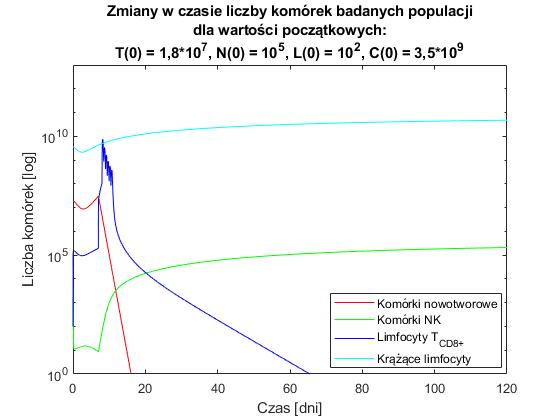
\includegraphics[width=0.45\textwidth]{wykres_skojarzone200}}
\quad
\subfloat[Zmiany w~czasie st�enia, dozowanego podczas leczenia skojarzonego, cytostatyka oraz~IL-2 dla~120-dniowego cyklu chemioterapii (w leczeniu skojarzonym).]{\label{stezenie_skojarzone200}
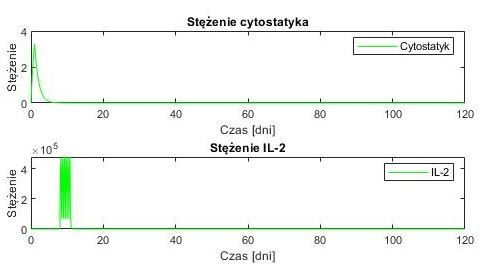
\includegraphics[width=0.45\textwidth]{stezenie_skojarzone200}}
\caption[Zmiany w~czasie liczby kom�rek badanych populacji oraz~st�enia cytostatyka i~IL-2 - leczenie skojarzonymi metodami chemioterapii i~immunoterapii, scenariusz I, zmiana d�ugo�ci cyklu]{Zmiany w~czasie liczby kom�rek badanych populacji oraz~st�enia, dozowanego podczas leczenia skojarzonego, cytostatyka oraz~IL-2 dla~120-dniowego cyklu chemioterapii. Pocz�tkowa liczba kom�rek nowotworowych $T(0) = 1,8 \cdot 10^{7}$, pocz�tkowa liczba kom�rek NK $N(0) = 10^{5}$, pocz�tkowa liczba limfocyt�w $T_{CD8+}$ $L(0) = 10^{2}$, pocz�tkowa liczba limfocyt�w kr���cych $C(0) = 3,5 \cdot 10^{9}$.}
\label{wykresy_skojarzone200}
\end{figure}

\newpage
Cz�� wynik�w symulacji w~formie graficznej, przedstawia Rys. \ref{slupki_9.1}.

\begin{figure}[h!]
\centering
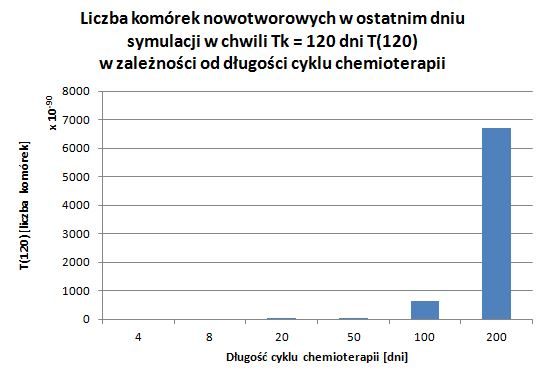
\includegraphics[width=0.8\textwidth]{slupki_9.1}
\caption{Liczba kom�rek nowotworowych $T(120)$  w ostatnim dniu symulacji w chwili $T_{k} = 120$ dni w zale�no�ci od d�ugo�ci cyklu chemioterapii w leczeniu skojarzonym.}\label{slupki_9.1}
\end{figure}

\newpage
\textbf{Wnioski:}
\begin{itemize}
\item zmiana d�ugo�ci cyklu chemioterapii w~leczeniu skojarzonym wp�ywa na~dzie� nast�pienia regresji nowotworu, natomiast powy�ej cyklu wynosz�cego 20 dni (w tym 1 dzie� dozowania cytostatyka i~reszta dni przerwy), d�ugo�� cyklu nie~powoduje op�nienia regresji i~zawsze wyst�puje ona w~17 dniu symulacji;
\item leczenie skojarzone z~chemioterapi� o~d�ugo�ci cyklu r�wnej 4 dni i~schemacie [1 3] prowadzi do~regresji nowotworu (dzie� regresji: 14) podobnie jak~w~przypadku leczenia wy��cznie metod� chemioterapii (dzie� regresji: 26), jednak regresja w~tym przypadku nast�puje du�o wcze�niej (12 dni), co~jest~oczywist� korzy�ci� dla~pacjenta;
\item leczenie skojarzone zawieraj�ce chemioterapi� o~d�ugo�ci cyklu r�wnej 8 dni i~schemacie [1 7] prowadzi do~regresji nowotworu (dzie� regresji: 15) co~by�o niemo�liwe w~przypadku leczenia wy��cznie metod� chemioterapii, ponadto regresja w~tym przypadku nast�puje zaledwie dzie� p�niej ni�~w~przypadku cyklu o~d�ugo�ci 4 dni przy dwukrotnie rzadszym dozowaniu cytostatyka;
\item leczenie skojarzone umo�liwia regresj� nowotworu nawet przy d�ugo�ci cyklu r�wnej 120 dni (co dla~symulacji wynosz�cej 120 dni jest r�wnoznaczne z~jednorazowym dozowaniem cytostatyka); dzi�ki leczeniu skojarzonemu mo�liwe jest~znaczne wyd�u�enie cyklu chemioterapii (tj. wyd�u�enie przerwy pomi�dzy kolejnymi dawkami cytostatyka) przy~zachowaniu skuteczno�ci leczenia, co~pozwala na~wi�ksz� regeneracj� zdrowych tkanek w~przerwach pomi�dzy kolejnymi dawkami cytostatyka lub~nawet ograniczenie leczenia do~podania pacjentowi pojedynczej dawki cytostatyka i~tym~samym oganiczenie skutk�w ubocznych chemioterapii.
\end{itemize}

\newpage
\subsection{Zmiana dawki dozowanego cytostatyka}

\begin{small}
Tab. \ref{zmiana_cehmio_stale_immuno_dawka} przedstawia zmiany dawki dozowanego cytostatyka $V_M$. Dodatkowo, w~tabeli zamieszczono dzie� regresji nowotworu oraz~liczb� kom�rek nowotworu T(120) w~ostatnim (120) dniu symulacji, a~tak�e~szacowan� obj�to�� i~d�ugo�� promienia nowotworu w~ostatnim (120) dniu symulacji (tj. w~chwili $T_{k}$ = 120 dni). Analiz� przeprowadzono dla~d�ugo�ci cyklu r�wnej: 4, 8 oraz~120 dni.
\end{small}

\begin{table}[h!]
\footnotesize
	\centering
	\caption[Wyniki symulacji - leczenie skojarzonymi metodami chemioterapii i~immunoterapii, scenariusz I, zmiana dawki dozowanego cytostatyka $V_M$]{Dawka dozowanego cytostatyka $V_M$, dzie� regresji nowotworu, liczba kom�rek nowotworowych T(120) w~ostatnim (120) dniu symulacji oraz~szacowana obj�to�� i~d�ugo�� promienia nowotworu w~ostatnim (120) dniu symulacji (tj. w~chwili $T_{k}$ = 120 dni) dla~immunoterapii o~warunkach pocz�tkowych (\ref{warunki_pocz�tkowe_immunoterapii}) dla~d�ugo�ci cyklu r�wnej 4, 8 oraz~120 dni.}
\label{zmiana_cehmio_stale_immuno_dawka}
\begin{tabular}{|c|c|c|c|c|} \hline \hline
        \multicolumn{5}{|c|}{\textbf{D�ugo�� cyklu: 4 dni}} \\ \hline \hline
		Dawka dozowanego & Dzie� & $T(120)$ & Obj�to�� & D�ugo�� promienia \\
		cytostatyka & regresji & $[liczba$ $kom$�$rek]$ & nowotworu & nowotworu \\ 
		$V_M$ $[\dfrac{mg}{m^{2}}]$ & nowotworu & & [$mm^{3}$] & [$mm$] \\ \hline
		5 & 13,25 & $9,43 \cdot 10^{-95}$ & $9,43 \cdot 10^{-101}$ & $2,8 \cdot 10^{-34}$ \\ \hline
		4 & 13,5 & $5,23 \cdot 10^{-94}$ & $5,23 \cdot 10^{-100}$ & $5 \cdot 10^{-34}$ \\ \hline
		3 & 13,92 & $1,25 \cdot 10^{-92}$ & $1,25 \cdot 10^{-98}$ & $1,4 \cdot 10^{-33}$ \\ \hline
		2 & 14,54 & $1,06 \cdot 10^{-90}$ & $1,06 \cdot 10^{-96}$ & $6,3 \cdot 10^{-33}$ \\ \hline
		1 & 16,5 & $3,08 \cdot 10^{-88}$ & $3,08 \cdot 10^{-94}$ & $4,2 \cdot 10^{-32}$ \\ \hline
		0,75 & 17,75 & $1,13 \cdot 10^{-86}$ & $1,13 \cdot 10^{-92}$ & $1,4 \cdot 10^{-31}$ \\ \hline
		0,5 & brak & $9,8 \cdot 10^{8}$ & $980$ & $6,16$ \\ \hline \hline
        \multicolumn{5}{|c|}{\textbf{D�ugo�� cyklu: 8 dni}} \\ \hline \hline
		Dawka dozowanego & Dzie� & $T(120)$ & Obj�to�� & D�ugo�� promienia \\
		cytostatyka & regresji & $[liczba$ $kom$�$rek]$ & nowotworu & nowotworu \\ 
		$V_M$ $[\dfrac{mg}{m^{2}}]$ & nowotworu & & [$mm^{3}$] & [$mm$] \\ \hline
		5 & 14,79 & $5,57 \cdot 10^{-95}$ & $5,57 \cdot 10^{-101}$ & $2,4 \cdot 10^{-34}$ \\ \hline
		4 & 15,08 & $5,05 \cdot 10^{-94}$ & $5,05 \cdot 10^{-100}$ & $4,9 \cdot 10^{-34}$ \\ \hline
		3 & 15,67 & $9,99 \cdot 10^{-93}$ & $9,99 \cdot 10^{-99}$ & $1,3 \cdot 10^{-33}$ \\ \hline
		2 & 16,92 & $2,95 \cdot 10^{-90}$ & $2,95 \cdot 10^{-96}$ & $8,9 \cdot 10^{-33}$ \\ \hline
		1,75 & 17,34 & $3,14 \cdot 10^{-89}$ & $3,14 \cdot 10^{-95}$ & $2 \cdot 10^{-32}$ \\ \hline
		1,5 & brak & $9,8 \cdot 10^{8}$ & $980$ & $6,16$ \\ \hline
		1 & brak & $9,8 \cdot 10^{8}$ & $980$ & $6,16$ \\ \hline  \hline
		 \multicolumn{5}{|c|}{\textbf{D�ugo�� cyklu: 120 dni}} \\ \hline \hline
		Dawka dozowanego & Dzie� & $T(120)$ & Obj�to�� & D�ugo�� promienia \\
		cytostatyka & regresji & $[liczba$ $kom$�$rek]$ & nowotworu & nowotworu \\ 
		$V_M$ $[\dfrac{mg}{m^{2}}]$ & nowotworu & & [$mm^{3}$] & [$mm$] \\ \hline
		5 & 16,08 & $6,71 \cdot 10^{-87}$ & $6,71 \cdot 10^{-93}$ & $1,2 \cdot 10^{-31}$ \\ \hline
		4 & 16,25 & $9,35 \cdot 10^{-87}$ & $9,35 \cdot 10^{-93}$ & $1,3 \cdot 10^{-31}$ \\ \hline
		3 & 16,63 & $1,94 \cdot 10^{-86}$ & $1,94 \cdot 10^{-92}$ & $1,7 \cdot 10^{-31}$ \\ \hline
		2 & 17,88 & $2,13 \cdot 10^{-85}$ & $2,13 \cdot 10^{-91}$ & $3,7 \cdot 10^{-31}$ \\ \hline
		1,75 & 19,42 & $3,92 \cdot 10^{-84}$ & $3,92 \cdot 10^{-90}$ & $9,8 \cdot 10^{-31}$ \\ \hline
		1,5 & brak & $9,8 \cdot 10^{8}$ & $980$ & $6,16$ \\ \hline
		\end{tabular}
\end{table} 

\newpage
Przyk�adowy wynik leczenia metodami skojarzonymi przedstawia Rys. \ref{wykresy_skojarzone_dawka1_75}. Ukazuje on~zmiany w~czasie liczby kom�rek badanych populacji, tj. kom�rek nowotworowych, kom�rek NK, limfocyt�w $T_{CD8+}$ oraz~limfocyt�w kr���cych dla~leczenia skojarzonego metodami chemioterapii i~immunoterapii, gdzie d�ugo�� cyklu chemioterapii wynosi 8 dni (Rys. \ref{wykres_skojarzone_dawka1_75}), a~tak�e zmiany w~czasie st�enia, dozowanego podczas leczenia skojarzonego, cytostatyka i~IL-2 (Rys. \ref{stezenie_skojarzone200}). 

Warunki pocz�tkowe immunoterapii przedstawia Tab. \ref{warunki_pocz�tkowe_immunoterapii}. Dawk� cytostatyka zmniejszono do~warto�ci $V_M = 1,75$ $\dfrac{mg}{m^{2}}$, poniewa� jest to~najmniejsza dawka skuteczna (powoduj�ca regresj� guza) przy niezmienionych pozosta�ych warto�ciach pocz�tkowych. Regresja wyst�pi�a w~18 dniu symulacji.

\begin{figure}[h!]
\centering
\subfloat[Zmiany w~czasie liczby kom�rek badanych populacji dla~8-dniowego cyklu chemioterapii oraz~dawki dozowanego cytostatyka $V_M = 1,75$ $\dfrac{mg}{m^{2}}$. Regresja nowotworu widoczna (linia czerwona) po~czasie $T_{r}$~$\approx$ 18 dni.]{\label{wykres_skojarzone_dawka1_75}
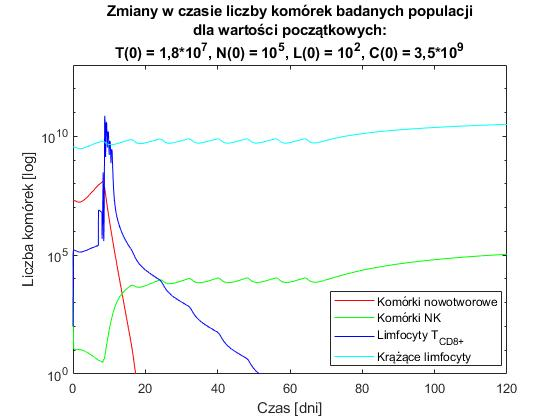
\includegraphics[width=0.45\textwidth]{wykres_skojarzone_dawka1_75}}
\quad
\subfloat[Zmiany w~czasie st�enia, dozowanego podczas leczenia skojarzonego, cytostatyka oraz~IL-2 dla~8-dniowego cyklu chemioterapii oraz~dawki dozowanego cytostatyka $V_M = 1,75$ $\dfrac{mg}{m^{2}}$.]{\label{stezenie_skojarzone_dawka1_75}
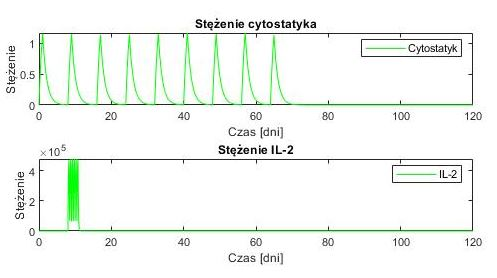
\includegraphics[width=0.45\textwidth]{stezenie_skojarzone_dawka1_75}}
\caption[Zmiany w~czasie liczby kom�rek badanych populacji oraz~st�enia cytostatyka i~IL-2 - leczenie skojarzonymi metodami chemioterapii i~immunoterapii, scenariusz I, zmiana dawki dozowanego cytostatyka $V_M$]{Zmiany w~czasie liczby kom�rek badanych populacji oraz~st�enia, dozowanego podczas leczenia skojarzonego, cytostatyka oraz~IL-2 dla~8-dniowego cyklu chemioterapii oraz~dawki dozowanego cytostatyka $V_M = 1,75$ $\dfrac{mg}{m^{2}}$. Pocz�tkowa liczba kom�rek nowotworowych $T(0) = 1,8 \cdot 10^{7}$, pocz�tkowa liczba kom�rek NK $N(0) = 10^{5}$, pocz�tkowa liczba limfocyt�w $T_{CD8+}$ $L(0) = 10^{2}$, pocz�tkowa liczba limfocyt�w kr���cych $C(0) = 3,5 \cdot 10^{9}$.}
\label{wykresy_skojarzone_dawka1_75}
\end{figure}

\newpage
Cz�� wynik�w symulacji w~formie graficznej, przedstawia Rys. \ref{slupki_9.2}.

\begin{figure}[h!]
\centering
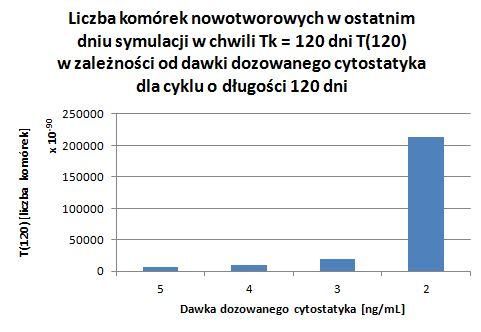
\includegraphics[width=0.8\textwidth]{slupki_9.2}
\caption{Liczba kom�rek nowotworowych $T(120)$  w ostatnim dniu symulacji w chwili $T_{k} = 120$ dni w zale�no�ci od dawki dozowanego cytostatyka $V_M$ w leczeniu skojarzonym.}\label{slupki_9.2}
\end{figure}

\textbf{Wnioski:}
\begin{itemize}
\item skuteczno�� leczenia skojarzonego zale�y od~wielko�ci dawki dozowanego w~chemioterapii cytostatyka; dla~kr�tkiego cyklu (4 dni) dawk� wystarczaj�c� do~osi�gni�cia zamierzonego efektu (regresji nowotworu) w~18 dniu symulacji jest $V_M = 0,75$ $\dfrac{mg}{m^{2}}$ (w przypadku leczenia wy��cznie metod� chemioterapii ta~dawka wynosi $V_M = 3,5$ $\dfrac{mg}{m^{2}}$ (Tab. \ref{chemio_zmiany_dawki}), czyli ponad cztery razy wi�cej, podczas gdy dzie� regresji to~50 dzie� symulacji), natomiast dla~d�u�szych cykli (8 oraz~120 dni) jest to~dawka $V_M = 1,75$ $\dfrac{mg}{m^{2}}$ (warto�� t� wykorzystano w~dalszych symulacjach), podczas gdy w~leczeniu wy��cznie metod� chemioterapii dla~cyklu o~d�ugo�ci 8 dni regresja nie~wyst�puje lub wyst�puje dla~bardzo du�ej warto�ci dawki ($V_M = 13$ $\dfrac{mg}{m^{2}}$); leczenie skojarzone umo�liwia osi�gni�cie regresji nowotworu, co~jest~nieosi�galne w~leczeniu wy��cznie metod� chemioterapii (dla takich samych warunk�w pocz�tkowych);
\item w~przypadku leczenia metodami skojarzonymi, dawka mo�e zosta� kilkakrotnie zmniejszona w~por�wnaniu do~leczenia wy��cznie metod� chemioterapii, co~zabezpiecza pacjenta przed~negatywnymi skutkami ubocznymi stosowania cytostatyk�w.
\end{itemize}

\newpage

\subsection{Zmiana liczby powt�rze� cyklu chemioterapii}

Tab. \ref{zmiana_cehmio_stale_immuno_liczba_powtorzen_cyklu} przedstawia zmiany liczby powt�rze� cyklu chemioterapii. Dodatkowo, w~tabeli umieszczono dzie� regresji nowotworu oraz~liczb� kom�rek nowotworu T(120) w~ostatnim (120) dniu symulacji, a~tak�e~szacowan� obj�to�� i~d�ugo�� promienia nowotworu w~ostatnim (120) dniu symulacji (tj. w~chwili $T_{k}$ = 120 dni). Analiz� przeprowadzono dla~d�ugo�ci cyklu r�wnej 8 dni (wybrano tak� d�ugo�� cyklu ze wzgl�du na~por�wnanie pozytywnego efektu (wyst�pienia regresji) leczenia skojarzonego dla~tej warto�ci z~brakiem wyst�pienia tego efektu w~leczeniu wy��cznie metod� chemioterapii dla~tej d�ugo�ci cyklu) oraz~dawki cytostatyka $V_M = 1,75$ $\dfrac{mg}{m^{2}}$ (analiz� przeprowadzono dla~takiej warto�ci dawki, poniewa� jest to~najmniejsza, a~tym samym najmniej szkodliwa dawka, przy kt�rej nast�puje regresja nowotworu dla~d�ugich cykli (8 oraz~120 dni)).

\begin{table}[h!]
\small
	\centering
	\caption[Wyniki symulacji - leczenie skojarzonymi metodami chemioterapii i~immunoterapii, scenariusz I, zmiana liczby powt�rze� cyklu chemioterapii]{Liczba powt�rze� cyklu chemioterapii, dzie� regresji nowotworu, liczba kom�rek nowotworowych T(120) w~ostatnim (120) dniu symulacji oraz~szacowana obj�to�� i~d�ugo�� promienia nowotworu w~ostatnim (120) dniu symulacji (tj. w~chwili $T_{k}$ = 120 dni) dla~immunoterapii o~warunkach pocz�tkowych (Tab. \ref{warunki_pocz�tkowe_immunoterapii}) dla~d�ugo�ci cyklu r�wnej 8 dni oraz~dawki cytostatyka $V_M = 1,75$ $\dfrac{mg}{m^{2}}$.}
\label{zmiana_cehmio_stale_immuno_liczba_powtorzen_cyklu}
\begin{tabular}{|c|c|c|c|c|} \hline \hline
        \multicolumn{5}{|c|}{D�ugo�� cyklu: 8 dni, $V_M = 1,75$ $\dfrac{mg}{m^{2}}$} \\ \hline \hline
		Liczba & Dzie� regresji & $T(120)$ & Obj�to�� & D�ugo�� promienia \\
		powt�rze� & nowotworu & $[liczba$ $kom$�$rek]$ & nowotworu [$mm^{3}$] & nowotworu [$mm$] \\ \hline
		9 & 17,34 & $3,14 \cdot 10^{-89}$ & $3,14 \cdot 10^{-95}$ & $2 \cdot 10^{-32}$ \\ \hline
		8 & 17,34 & $1,1 \cdot 10^{-88}$ & $1,1 \cdot 10^{-94}$ & $3 \cdot 10^{-32}$ \\ \hline
		7 & 17,34 & $3,59 \cdot 10^{-88}$ & $3,59 \cdot 10^{-94}$ & $4,4 \cdot 10^{-32}$ \\ \hline
		6 & 17,34 & $1,23 \cdot 10^{-87}$ & $1,23 \cdot 10^{-93}$ & $6,7 \cdot 10^{-32}$ \\ \hline
		5 & 17,34 & $2,91 \cdot 10^{-87}$ & $2,91 \cdot 10^{-93}$ & $8,9 \cdot 10^{-32}$ \\ \hline
		4 & 17,34 & $1,06 \cdot 10^{-86}$ & $1,06 \cdot 10^{-92}$ & $1,4 \cdot 10^{-31}$ \\ \hline
		3 & 17,34 & $3,85 \cdot 10^{-86}$ & $3,85 \cdot 10^{-92}$ & $2,1 \cdot 10^{-31}$ \\ \hline
		2 & 17,67 & $1,41 \cdot 10^{-85}$ & $1,41 \cdot 10^{-91}$ & $3,2 \cdot 10^{-31}$ \\ \hline
		1 & 19,42 & $3,92 \cdot 10^{-84}$ & $3,92 \cdot 10^{-90}$ & $9,8 \cdot 10^{-31}$ \\ \hline
		\end{tabular}
\end{table} 

Przyk�adowy wynik symulacji przedstawia Rys. \ref{wykresy_skojarzone_l_powt1}, kt�ry ukazuje zmiany w~czasie liczby kom�rek badanych populacji, tj. kom�rek nowotworowych, kom�rek NK, limfocyt�w $T_{CD8+}$ oraz~limfocyt�w kr���cych dla~leczenia skojarzonego metodami chemioterapii i~immunoterapii, gdzie d�ugo�� cyklu chemioterapii wynosi�a 8 dni (Rys. \ref{wykres_skojarzone_l_powt1}), a~tak�e zmiany w~czasie st�enia, dozowanego podczas leczenia skojarzonego, cytostatyka i~IL-2 (Rys. \ref{stezenie_skojarzone_l_powt1}). 

\newpage
Warunki pocz�tkowe immunoterapii przedstawia Tab. \ref{warunki_pocz�tkowe_immunoterapii}. Dawka cytostatyka wynosi�a $V_M = 1,75$ $\dfrac{mg}{m^{2}}$. Ju� jeden cykl chemioterapii skutkowa� regresj� nowotworu w~20 dniu symulacji (Rys. \ref{wykres_skojarzone_l_powt1}).

\begin{figure}[h!]
\centering
\subfloat[Zmiany w~czasie liczby kom�rek badanych populacji dla~8-dniowego cyklu chemioterapii, dawki dozowanego cytostatyka $V_M = 1,75$ $\dfrac{mg}{m^{2}}$ oraz~jednokrotnego cyklu chemioteapii. Widoczna (linia czerwona) regresja nowotworu po~20 dniach.]{\label{wykres_skojarzone_l_powt1}
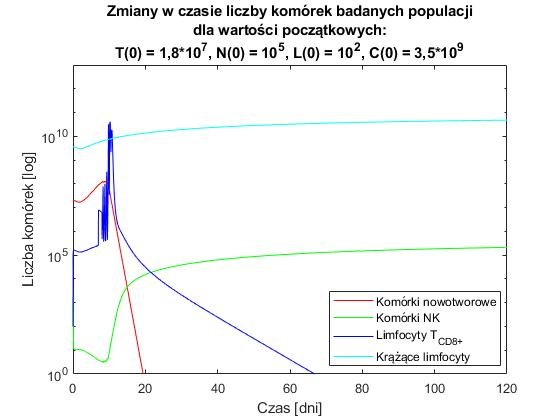
\includegraphics[width=0.45\textwidth]{wykres_skojarzone_l_powt1}}
\quad
\subfloat[Zmiany w~czasie st�enia, dozowanego podczas leczenia skojarzonego, cytostatyka oraz~IL-2 dla~8-dniowego cyklu chemioterapii, dawki dozowanego cytostatyka $V_M = 1,75$ $\dfrac{mg}{m^{2}}$ oraz~pojedynczego cyklu chemioterapii.]{\label{stezenie_skojarzone_l_powt1}
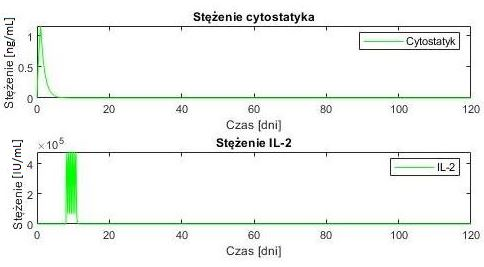
\includegraphics[width=0.45\textwidth]{stezenie_skojarzone_l_powt1}}
\caption[Zmiany w~czasie liczby kom�rek badanych populacji oraz~st�enia cytostatyka i~IL-2 - leczenie skojarzonymi metodami chemioterapii i~immunoterapii, scenariusz I, zmiana liczby powt�rze� cyklu chemioterapii]{Zmiany w~czasie liczby kom�rek badanych populacji oraz~st�enia, dozowanego podczas leczenia skojarzonego, cytostatyka oraz~IL-2 dla~8-dniowego cyklu chemioterapii, dawki dozowanego cytostatyka $V_M = 1,75$ $\dfrac{mg}{m^{2}}$ pojedynczego cyklu chemioterapii. Pocz�tkowa liczba kom�rek nowotworowych $T(0) = 1,8 \cdot 10^{7}$, pocz�tkowa liczba kom�rek NK $N(0) = 10^{5}$, pocz�tkowa liczba limfocyt�w $T_{CD8+}$ $L(0) = 10^{2}$, pocz�tkowa liczba limfocyt�w kr���cych $C(0) = 3,5 \cdot 10^{9}$.}
\label{wykresy_skojarzone_l_powt1}
\end{figure}

\newpage
Cz�� wynik�w symulacji w~formie graficznej, przedstawia Rys. \ref{slupki_9.3}.

\begin{figure}[h!]
\centering
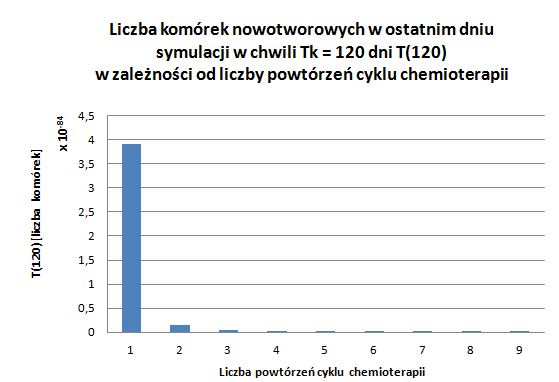
\includegraphics[width=0.8\textwidth]{slupki_9.3}
\caption{Liczba kom�rek nowotworowych $T(120)$ w ostatnim dniu symulacji w chwili $T_{k} = 120$ dni w zale�no�ci od liczby powt�rze� cyklu chemioterapii w leczeniu skojarzonym.}\label{slupki_9.3}
\end{figure}

\textbf{Wnioski:}
\begin{itemize}
\item liczba powt�rze� cyklu nie~ma~wp�ywu na~skuteczno�� leczenia (wyst�pienie regresji nowotworu) w~leczeniu skojarzonym; zar�wno dla~9 powt�rze� (podobnie jak~we wcze�niejszych symulacjach dla~leczenia wy��cznie metod� chemioterapii oraz~wy��cznie metod� immunoterapii), jak~i~dla pojedynczego cyklu dozowania cytostatyka (brak regresji we wcze�niejszych symulacjach) nast�puje regresja nowotworu;
\item liczba powt�rze� cyklu nie~wp�ywa lub wp�ywa nieznacznie na~czas wyst�pienia regresji, dla~3 do~9 powt�rze� jest to~dok�adnie ten~sam moment (dzie� 18), dla~2 powt�rze� ten~sam dzie�, jednak nieznacznie p�niej, natomiast dla~1 powt�rzenia cyklu dniem regresji nowotworu jest 20 dzie� symulacji.
\end{itemize}

\newpage
\subsection{Zmiana dnia rozpocz�cia chemioterapii}

Tab. \ref{zmiana_cehmio_stale_immuno_dzien_rozpoczecia} przedstawia zmiany dnia rozpocz�cia chemioterapii. Ponadto, tabela przedstawia dzie� regresji nowotworu oraz~liczb� kom�rek nowotworu T(120) w~ostatnim (120) dniu symulacji. Dodatkowo, w~tabeli umieszczono szacowan� obj�to�� i~d�ugo�� promienia nowotworu w~ostatnim (120) dniu symulacji (tj. w~chwili $T_{k}$ = 120 dni). Analiz� przeprowadzono dla~8-dniowego cyklu, dawki cytostatyka $V_M = 1,75$ $\dfrac{mg}{m^{2}}$ oraz~pojedynczego cyklu dozowania.

\begin{table}[h!]
	\centering
	\caption[Wyniki symulacji - leczenie skojarzonymi metodami chemioterapii i~immunoterapii, scenariusz I, zmiana dnia rozpocz�cia chemioterapii]{Dzie� rozpocz�cia chemioterapii, dzie� regresji nowotworu, liczba kom�rek nowotworowych T(120) w~ostatnim (120) dniu symulacji oraz~szacowana obj�to�� i~d�ugo�� promienia nowotworu w~ostatnim (120) dniu symulacji (tj. w~chwili $T_{k}$ = 120 dni) dla~immunoterapii o~warunkach pocz�tkowych (\ref{warunki_pocz�tkowe_immunoterapii}) dla~d�ugo�ci cyklu r�wnej 8 dni, dawki cytostatyka $V_M = 1,75$ $\dfrac{mg}{m^{2}}$ oraz~pojedynczego cyklu dozowania.}
\begin{tabular}{|c|c|c|c|c|} \hline \hline
\multicolumn{5}{|c|}{D�ugo�� cyklu: 8 dni, $V_M = 1,75$ $\dfrac{mg}{m^{2}}$, liczba powt�rze� cyklu: 1} \\ \hline \hline
		Dzie� & Dzie� & $T(120)$ & Obj�to�� & D�ugo�� promienia \\
		rozpocz�cia & regresji & $[liczba$ $kom$�$rek]$ & nowotworu & nowotworu \\
		chemioterapii & nowotworu & & [$mm^{3}$] & [$mm$]\\ \hline
		1 & 19,42 & $3,92 \cdot 10^{-84}$ & $3,92 \cdot 10^{-84}$ & $9,8 \cdot 10^{-31}$ \\ \hline
		2 & brak & $9,8 \cdot 10^{8}$ & $980$ & $6,16$ \\ \hline
		\end{tabular}
\label{zmiana_cehmio_stale_immuno_dzien_rozpoczecia}
\end{table} 

Przyk�adowy wynik symulacji przedstawia Rys. \ref{wykresy_skojarzone_l_powt1_drozp2}. S�~to~zmiany w~czasie liczby kom�rek badanych populacji, tj. kom�rek nowotworowych, kom�rek NK, limfocyt�w $T_{CD8+}$ oraz~limfocyt�w kr���cych dla~leczenia skojarzonego metodami chemioterapii i~immunoterapii, gdzie d�ugo�� cyklu chemioterapii wynosi 8 dni (Rys. \ref{wykres_skojarzone_l_powt1_drozp2}), a~tak�e zmiany w~czasie st�enia, dozowanego podczas leczenia skojarzonego, cytostatyka i~IL-2 (Rys. \ref{stezenie_skojarzone_l_powt1_drozp2}). 

Warunki pocz�tkowe immunoterapii przedstawia Tab. \ref{warunki_pocz�tkowe_immunoterapii}. Dawka cytostatyka wynosi�a $V_M = 1,75$ $\dfrac{mg}{m^{2}}$. Stosowano pojedynczy cykl chemioterapii.

\newpage
Dla podanych warunk�w chemioterapii, op�nienie rozpocz�cia leczenia o~1 dzie� skutkuje brakiem regresji nowotworu i~stabilizacj� kom�rek nowotworowych w~32 dniu symulacji na~poziomie $9,8 \cdot 10^{8}$.

\begin{figure}[h!]
\centering
\subfloat[Zmiany w~czasie liczby kom�rek badanych populacji dla~8-dniowego cyklu chemioterapii, dawki dozowanego cytostatyka $V_M = 1,75$ $\dfrac{mg}{m^{2}}$, pojedynczego cyklu dozowania oraz~chemioterapii rozpocz�tej 2 dnia. Widoczna (linia czerwona) stabilizacja liczby kom�rek nowotworowych po~32 dniach oko�o warto�ci $9,8 \cdot 10^{8}$.]{\label{wykres_skojarzone_l_powt1_drozp2}
\includegraphics[width=0.45\textwidth]{wykres_skojarzone_l_powt1_drozp2}}
\quad
\subfloat[Zmiany w~czasie st�enia, dozowanego podczas leczenia skojarzonego, cytostatyka oraz~IL-2 dla~8-dniowego cyklu chemioterapii, dawki dozowanego cytostatyka $V_M = 1,75$ $\dfrac{mg}{m^{2}}$, pojedynczego cyklu dozowania oraz~chemioterapii rozpocz�tej 2 dnia.]{\label{stezenie_skojarzone_l_powt1_drozp2}
\includegraphics[width=0.45\textwidth]{stezenie_skojarzone_l_powt1_drozp2}}
\caption[Zmiany w~czasie liczby kom�rek badanych populacji oraz~st�enia cytostatyka i~IL-2 - leczenie skojarzonymi metodami chemioterapii i~immunoterapii, scenariusz I, zmiana dnia rozpocz�cia chemioterapii]{Zmiany w~czasie liczby kom�rek badanych populacji oraz~st�enia dozowanego podczas leczenia skojarzonego cytostatyka oraz~IL-2 dla~8-dniowego cyklu chemioterapii, dawki dozowanego cytostatyka $V_M = 1,75$ $\dfrac{mg}{m^{2}}$, pojedynczego cyklu dozowania oraz~chemioterapii rozpocz�tej 2 dnia. Pocz�tkowa liczba kom�rek nowotworowych $T(0) = 1,8 \cdot 10^{7}$, pocz�tkowa liczba kom�rek NK $N(0) = 10^{5}$, pocz�tkowa liczba limfocyt�w $T_{CD8+}$ $L(0) = 10^{2}$, pocz�tkowa liczba limfocyt�w kr���cych $C(0) = 3,5 \cdot 10^{9}$.}
\label{wykresy_skojarzone_l_powt1_drozp2}
\end{figure}

\textbf{Wnioski:}
\begin{itemize}
\item leczenie skojarzone dla~warunk�w pocz�tkowych immunoterapii (Tab. \ref{warunki_pocz�tkowe_immunoterapii}) daje pozytywny skutek (rozumiany jako regresja nowotworu) dla~rozwa�anego typu chemioterapii (d�ugo�� cyklu = 8 dni, dawka cytostatyka $V_M = 1,75$ $\dfrac{mg}{m^{2}}$, liczba powt�rze� cyklu: 1) tylko w~przypadku, gdy pierwszy dzie� symulacji jest r�wnocze�nie pierwszym dniem leczenia (rozpocz�cie dozowania cytostatyka nast�puje w~pierwszym dniu symulacji); chemioterapia dla~rozwa�anych warunk�w jest~wi�c~ograniczona (przy warunkach pocz�tkowych immunoterapii) tak, aby~otrzyma� oczekiwany efekt przy~jednoczesnych jak~najmniejszych skutkach ubocznych chemioterapii (kt�re mog� by� spowodowane zbyt du�� dawk� cytostatyka czy~d�ugim czasem leczenia metod� chemioterapii).
\end{itemize}

Leczenie skojarzone metodami chemioterapii i~immunoterapii umo�liwia zniszczenie nowotworu dla~warunk�w, dla~kt�rych nie~jest to~mo�liwe przy zastosowaniu tych terapii osobno, co~pokazuje przewag� leczenia skojarzonego nad pozosta�ymi metodami. Poza umo�liwieniem regresji nowotworu, leczenie skojarzone znacznie skraca czas konieczny do~jej wyst�pienia. Dzi�ki w��czeniu do~leczenia immunoterapii, mo�liwe jest r�wnie�~znaczne ograniczenie bardziej szkodliwej dla~organizmu chemioterapii, np. wyd�u�enie cyklu chemioterapii (nawet do~120 dni), ograniczenie dawki cytostatyka $V_M =5$ $\dfrac{mg}{m^{2}}$ do~$V_M = 1,75$ $\dfrac{mg}{m^{2}}$ oraz~za�o�enie pojedynczego cyklu dozowania cytostatyka (zamiast 9 powt�rze�). Leczenie (od dnia dozowania cytostatyka do~dnia regresji nowotworu) w~takim przypadku trwa 20 dni, zak�adaj�c rozpocz�cie leczenia w~pierwszym dniu symulacji.

\newpage
\section{Scenariusz II -- zmiana warunk�w pocz�tkowych immunoterapii}

\noindent \textbf{Podejmowany problem:} \newline Zmiany warunk�w pocz�tkowych immunoterapii, tj. dawki IL-2, liczby powt�rze� cyklu IL-2 oraz~dnia rozpocz�cia immunoterapii (dozowania IL-2) przy~sta�ych warunkach pocz�tkowych chemioterapii.

\noindent \newline \textbf{Warunki pocz�tkowe:} 
\begin{itemize}
\item dla~pocz�tkowej wielko�ci badanych populacji, tj. pocz�tkow� liczb� kom�rek nowotworu $T(0)$, liczb� kom�rek NK $N(0)$, liczb� limfocyt�w $T_{CD8+}$ oraz~liczb� limfocyt�w kr���cych $C(0)$ przedstawia Tab. \ref{warunki_poczatkowe_z1};
\item dla~chemioterapii, tj. d�ugo�� cyklu, czas dozowania cytostatyka, schemat cyklu, dawk� dozowanego cytostatyka, liczb� powt�rze� cyklu oraz~dzie� rozpocz�cia chemioterapii przedstawia Tab. \ref{warunki_pocz�tkowe_chemioterapii_w_skojarzonym_ze_zmiana_immuno};
\item dla~immunoterapii, tj. d�ugo�� cyklu, czas dozowania, schemat cyklu, dawk� dozowanych lek�w (IL-2 i TIL), liczb� powt�rze� cyklu oraz~dzie� rozpocz�cia immunoterapii przedstawia Tab. \ref{warunki_pocz�tkowe_immunoterapii}.
\end{itemize}

\begin{table}[h!]
\small
	\centering
	\caption{Warunki pocz�tkowe modelu odpowiedzi immunologicznej na~rozwijaj�cy si� nowotw�r z~uwzgl�dnieniem procesu leczenia za~pomoc� chemioterapii.}\label{warunki_pocz�tkowe_chemioterapii_w_skojarzonym_ze_zmiana_immuno}
\begin{tabular}{|c|c|c|c|c|c|} \hline
		D�ugo�� & Czas dozowania & Schemat & Dawka & Liczba & Dzie� \\
		cyklu & cytostatyka & cyklu & dozowanego & powt�rze� & rozpocz�cia \\
		$[dni]$ & $[dni]$ & [dozowanie & cytostatyka & cyklu & chemioterapii \\ 
		 & &  przerwa] & $V_M$ $[\dfrac{mg}{m^{2}}]$ &  &  \\ \hline 
		8 & 1 & [1 7] & 5 & 9 & 1 \\ \hline
		\end{tabular}
\end{table} 

\noindent \newline \textbf{Przyj�te parametry:} \newline Parametry dla~modelu uwzgl�dniaj�cego leczenie przedstawia Tab. \ref{parametry_modelu_bez1} i~\ref{parametry_modelu_z1}.

\noindent \newline \textbf{Czas symulacji:} \newline Czas symulacji wynosi� $T_{k}$ = 120 dni. 

\noindent \newline \textbf{Wyniki symulacji:} \newline Wyniki przeprowadzonych symulacji dla~zmieniaj�cych si� warunk�w pocz�tkowych immunoterapii przy sta�ej warto�ci warunk�w pocz�tkowych chemioterapii zebrano w~Tab. \ref{zmiana_immuno_stale_chemio_dawka_IL2_z_TIL} - \ref{zmiana_immuno_stale_chemio_dzien_rozpoczecia_IL2_bez_TIL}.

\newpage
\subsection{Zmiana dawki IL-2} \label{z_til_zawsze_skuteczne}

Tab. \ref{zmiana_immuno_stale_chemio_dawka_IL2_z_TIL} przedstawia zmiany dawki IL-2 $V_I$. Ponadto, zamieszczono w~niej dzie� regresji nowotworu oraz~liczb� kom�rek nowotworu T(120) w~ostatnim (120) dniu symulacji. Dodatkowo, w~tabeli umieszczono szacowan� obj�to�� i~d�ugo�� promienia nowotworu w~ostatnim (120) dniu symulacji (tj. w~chwili $T_{k}$ = 120 dni). Analiz� przeprowadzono dla~leczenia z~wykorzystaniem oraz~bez wykorzystania TIL.

\begin{table}[h!]
	\centering
	\caption[Wyniki symulacji - leczenie skojarzonymi metodami chemioterapii i~immunoterapii, scenariusz II, zmiana dawki IL-2 $V_I$]{Dawka IL-2 $V_I$, dzie� regresji nowotworu, liczba kom�rek nowotworowych T(120) w~ostatnim (120) dniu symulacji oraz~szacowana obj�to�� i~d�ugo�� promienia nowotworu w~ostatnim (120) dniu symulacji (tj. w~chwili $T_{k}$ = 120 dni) dla~chemioterapii o~warunkach pocz�tkowych (\ref{warunki_pocz�tkowe_chemioterapii_w_skojarzonym_ze_zmiana_immuno}) i~leczenia z~wykorzystaniem oraz~bez wykorzystania TIL.}
\label{zmiana_immuno_stale_chemio_dawka_IL2_z_TIL}
\begin{tabular}{|c|c|c|c|c|} \hline \hline
 \multicolumn{5}{|c|}{Leczenie z~wykorzystaniem TIL} \\ \hline \hline
		Dawka & Dzie� regresji & $T(120)$ & Obj�to�� & D�ugo�� promienia \\
		IL-2 $V_I$ $[\dfrac{IU}{kg}]$ & nowotworu & $[liczba$ $kom$�$rek]$ & nowotworu [$mm^{3}$] & nowotworu [$mm$] \\ \hline
		$5 \cdot 10^{6}$ & 14,79 & $5,57 \cdot 10^{-95}$ & $5,57 \cdot 10^{-101}$ & $1,4 \cdot 10^{-34}$ \\ \hline
		$1 \cdot 10^{6}$ & 14,79 & $5,46 \cdot 10^{-95}$ & $5,46 \cdot 10^{-101}$ & $2,4 \cdot 10^{-34}$ \\ \hline
		$9 \cdot 10^{5}$ & 14,79 & $3,06 \cdot 10^{-95}$ & $3,06 \cdot 10^{-101}$ & $1,9 \cdot 10^{-34}$ \\ \hline
		$0$ & 14,79 & $6,7 \cdot 10^{-35}$ & $6,7 \cdot 10^{-41}$ & $2,5 \cdot 10^{-14}$ \\ \hline \hline
		 \multicolumn{5}{|c|}{Leczenie bez wykorzystania TIL} \\ \hline \hline
		Dawka & Dzie� regresji & $T(120)$ & Obj�to�� & D�ugo�� promienia \\
		IL-2 $V_I$ $[\dfrac{IU}{kg}]$ & nowotworu & $[liczba$ $kom$�$rek]$ & nowotworu [$mm^{3}$] & nowotworu [$mm$] \\ \hline
		$5 \cdot 10^{6}$ & 16,08 & $3,69 \cdot 10^{-94}$ & $3,69 \cdot 10^{-100}$ & $4,5 \cdot 10^{-34}$ \\ \hline
		$4 \cdot 10^{6}$ & 16,08 & $5,93 \cdot 10^{-94}$ & $5,93 \cdot 10^{-100}$ & $5,2 \cdot 10^{-34}$ \\ \hline
		$3 \cdot 10^{6}$ & 16,13 & $6,64 \cdot 10^{-94}$ & $6,64 \cdot 10^{-100}$ & $5,4 \cdot 10^{-34}$ \\ \hline
		$2 \cdot 10^{6}$ & 16,42 & $8,32 \cdot 10^{-94}$ & $8,32 \cdot 10^{-100}$ & $5,8 \cdot 10^{-34}$ \\ \hline
		$1 \cdot 10^{6}$ & brak & $9,8 \cdot 10^{8}$ & $980$ & $6,16$ \\ \hline
		\end{tabular}
\end{table} 

Przyk�adowy wynik symulacji przedstawia Rys. \ref{wykresy_zmiana_immuno_stale_chemio_dawka_IL2_z_TIL}, kt�ry ukazuje zmiany w~czasie liczby kom�rek badanych populacji, tj. kom�rek nowotworowych, kom�rek NK, limfocyt�w $T_{CD8+}$ oraz~limfocyt�w kr���cych dla~leczenia skojarzonego metodami chemioterapii i~immunoterapii, dla~8-dniowego cyklu chemioterapii i~dawki IL-2 $V_I = 1 \cdot 10^{6}$ $\dfrac{IU}{kg}$ (Rys. \ref{wykres_zmiana_immuno_stale_chemio_dawka_IL2_z_TIL}) oraz~$V_I = 2 \cdot 10^{6}$ $\dfrac{IU}{kg}$ (Rys. \ref{wykres_zmiana_immuno_stale_chemio_dawka_IL2_z_TIL2e6}), a~tak�e zmiany w~czasie st�enia, dozowanego podczas leczenia skojarzonego, cytostatyka i~IL-2 (Rys. \ref{stezenie_zmiana_immuno_stale_chemio_dawka_IL2_z_TIL} i~Rys. \ref{stezenie_zmiana_immuno_stale_chemio_dawka_IL2_z_TIL2e6}). 

Pozosta�e warunki pocz�tkowe chemioterapii przedstawia Tab. \ref{warunki pocz�tkowe_chemioterapii}. Symulacja nie~obejmowa�a leczenia z~wykorzystaniem TIL. Dawk� IL-2 zmniejszono do~warto�ci $V_I = 2 \cdot 10^{6}$ $\dfrac{IU}{kg}$, poniewa� jest to~najmniejsza dawka skuteczna (powoduj�ca regresj� guza) przy niezmienionych pozosta�ych warto�ciach pocz�tkowych. Regresja wyst�pi�a w~17 dniu symulacji.

\begin{figure}[h!]
\centering
\subfloat[Zmiany w~czasie liczby kom�rek badanych populacji dla~8-dniowego cyklu chemioterapii, dawki IL-2 $V_I = 1 \cdot 10^{6}$ $\dfrac{IU}{kg}$ oraz~leczenia bez wykorzystania TIL. Widoczna (linia czerwona) stabilizacja liczby kom�rek nowotworu po~80 dniach.]{\label{wykres_zmiana_immuno_stale_chemio_dawka_IL2_z_TIL}
\includegraphics[width=0.45\textwidth]{beztil}}
\quad
\subfloat[Zmiany w~czasie st�enia, dozowanego podczas leczenia skojarzonego, cytostatyka oraz~IL-2 dla~8-dniowego cyklu chemioterapii, dawki IL-2 $V_I = 1 \cdot 10^{6}$ $\dfrac{IU}{kg}$ oraz~leczenia bez wykorzystania TIL.]{\label{stezenie_zmiana_immuno_stale_chemio_dawka_IL2_z_TIL}
\includegraphics[width=0.45\textwidth]{stezeniebeztil}}
\quad
\subfloat[Zmiany w~czasie liczby kom�rek badanych populacji dla~8-dniowego cyklu chemioterapii, dawki IL-2 $V_I = 2 \cdot 10^{6}$ $\dfrac{IU}{kg}$ oraz~leczenia bez wykorzystania TIL. Widoczna (linia czerwona) regresja nowotworu po~17 dniach.]{\label{wykres_zmiana_immuno_stale_chemio_dawka_IL2_z_TIL2e6}
\includegraphics[width=0.45\textwidth]{wykres_zmiana_immuno_stale_chemio_dawka_IL2_z_TIL2e6}}
\quad
\subfloat[Zmiany w~czasie st�enia, dozowanego podczas leczenia skojarzonego, cytostatyka oraz~IL-2 dla~8-dniowego cyklu chemioterapii, dawki IL-2 $V_I = 2 \cdot 10^{6}$ $\dfrac{IU}{kg}$ oraz~leczenia bez wykorzystania TIL.]{\label{stezenie_zmiana_immuno_stale_chemio_dawka_IL2_z_TIL2e6}
\includegraphics[width=0.45\textwidth]{stezenie_zmiana_immuno_stale_chemio_dawka_IL2_z_TIL2e6}}
\caption[Zmiany w~czasie liczby kom�rek badanych populacji oraz~st�enia cytostatyka i~IL-2 - leczenie skojarzonymi metodami chemioterapii i~immunoterapii, scenariusz II, zmiana dawki IL-2 $V_I$]{Zmiany w~czasie liczby kom�rek badanych populacji oraz~st�enia dozowanego podczas leczenia skojarzonego cytostatyka oraz~IL-2 dla~8-dniowego cyklu chemioterapii, dawki IL-2 $V_I = 1 \cdot 10^{6}$ $\dfrac{IU}{kg}$ i~$V_I = 2 \cdot 10^{6}$ $\dfrac{IU}{kg}$ oraz~leczenia bez wykorzystania TIL. Pocz�tkowa liczba kom�rek nowotworowych $T(0) = 1,8 \cdot 10^{7}$, pocz�tkowa liczba kom�rek NK $N(0) = 10^{5}$, pocz�tkowa liczba limfocyt�w $T_{CD8+}$ $L(0) = 10^{2}$, pocz�tkowa liczba limfocyt�w kr���cych $C(0) = 3,5 \cdot 10^{9}$.}
\label{wykresy_zmiana_immuno_stale_chemio_dawka_IL2_z_TIL}
\end{figure}

\newpage
Cz�� wynik�w symulacji w~formie graficznej, przedstawia Rys. \ref{slupki_9.6}.

\begin{figure}[h!]
\centering
\includegraphics[width=0.8\textwidth]{slupki_9.6}
\caption{Liczba kom�rek nowotworowych $T(120)$ w ostatnim dniu symulacji w chwili $T_{k} = 120$ dni w zale�no�ci od dawki IL-2 $V_I$ w leczeniu skojarzonym.}\label{slupki_9.6}
\end{figure}

\textbf{Wnioski:}
\begin{itemize}
\item w~leczeniu z~wykorzystaniem TIL wielko�� dawki IL-2 nie~wp�ywa na~skuteczno�� (wyst�pienie regresji nowotworu) terapii skojarzonej; niezale�nie od~wielko�ci dawki IL-2 regresja nast�puje w~15 dniu symulacji;
\item mo�liwe jest osi�gni�cie regresji nowotworu bez udzia�u IL-2 w~leczeniu, je�li zastosowano TIL oraz~chemioterapi� zgodnie z~warunkami pocz�tkowymi (Tab. \ref{warunki_pocz�tkowe_immunoterapii}, \ref{warunki_pocz�tkowe_chemioterapii_w_skojarzonym_ze_zmiana_immuno});
\item w~leczeniu bez wykorzystania TIL skuteczno�� (wyst�pienie regresji nowotworu) terapii skojarzonej zale�y od~wielko�ci dawki IL-2 (regresja dla~dawki $V_I = 2 \cdot 10^{6}$ $\dfrac{IU}{kg}$ (Rys. \ref{wykres_zmiana_immuno_stale_chemio_dawka_IL2_z_TIL2e6}), brak regresji dla~dawki $V_I = 1 \cdot 10^{6}$ $\dfrac{IU}{kg}$), natomiast moment wyst�pienia regresji zmienia si� nieznacznie zale�nie od~wybranej dawki.
\end{itemize}

\newpage
\subsection{Zmiana liczby powt�rze� cyklu IL-2 dla~leczenia bez~wykorzystania TIL}

Tab. \ref{zmiana_immuno_stale_chemio_powtorzenia_IL2_bez_TIL} przedstawia zmiany liczby powt�rze� cyklu IL-2. Dodatkowo w~tabeli umieszczono dzie� regresji nowotworu oraz~liczb� kom�rek nowotworu T(120) w~ostatnim (120) dniu symulacji, a~tak�e szacowan� obj�to�� i~d�ugo�� promienia nowotworu w~ostatnim (120) dniu symulacji (tj. w~chwili $T_{k}$ = 120 dni). Analiz� przeprowadzono dla~leczenia bez wykorzystania TIL w~celu sprawdzenia skuteczno�ci terapii z~wykorzystaniem wy��cznie IL-2 (jak wykazano w~symulacji \ref{z_til_zawsze_skuteczne}, leczenie wykorzystuj�ce TIL jest skuteczne w~ka�dym przypadku dla~podanych warunk�w pocz�tkowych \ref{warunki_pocz�tkowe_immunoterapii}) oraz~dawki IL-2 $V_I = 2 \cdot 10^{6}$ $\dfrac{IU}{kg}$ (najmniejszej dawki, przy kt�rej mo�liwe jest zniszczenie (regresja) nowotworu).

\begin{table}[h!]
	\centering
	\caption[Wyniki symulacji - leczenie skojarzonymi metodami chemioterapii i~immunoterapii, scenariusz II, zmiana liczby powt�rze� cyklu IL-2 dla~leczenia bez wykorzystania TIL]{Liczba powt�rze� cyklu IL-2, dzie� regresji nowotworu, liczba kom�rek nowotworowych T(120) w~ostatnim (120) dniu symulacji oraz~szacowana obj�to�� i~d�ugo�� promienia nowotworu w~ostatnim (120) dniu symulacji (tj. w~chwili $T_{k}$ = 120 dni) dla~chemioterapii o~warunkach pocz�tkowych (\ref{warunki_pocz�tkowe_chemioterapii_w_skojarzonym_ze_zmiana_immuno}) dla~leczenia bez wykorzystania TIL oraz~dawki IL-2 $V_I = 2 \cdot 10^{6}$ $\dfrac{IU}{kg}$.}
\label{zmiana_immuno_stale_chemio_powtorzenia_IL2_bez_TIL}
\begin{tabular}{|c|c|c|c|c|} \hline \hline
        \multicolumn{5}{|c|}{Leczenie bez wykorzystania TIL, $V_I = 2 \cdot 10^{6}$ $\dfrac{IU}{kg}$} \\ \hline \hline
		Liczba & Dzie� & $T(120)$ & Obj�to�� & D�ugo�� promienia \\
		powt�rze� & regresji & $[liczba$ $kom$�$rek]$ & nowotworu & nowotworu \\
		cyklu IL-2 & nowotworu & & [$mm^{3}$] & [$mm$] \\ \hline
		6 & 16,42 & $7,7 \cdot 10^{-94}$ & $7,7 \cdot 10^{-100}$ & $5,7 \cdot 10^{-34}$ \\ \hline
		4 & 16,42 & $7,18 \cdot 10^{-94}$ & $7,18 \cdot 10^{-100}$ & $5,6 \cdot 10^{-34}$ \\ \hline
		3 & 16,42 & $2,19 \cdot 10^{-93}$ & $2,19 \cdot 10^{-100}$ & $3,7 \cdot 10^{-34}$ \\ \hline
		2 & 16,42 & $1,4 \cdot 10^{-93}$ & $1,4 \cdot 10^{-100}$ & $3,2 \cdot 10^{-34}$ \\ \hline
		1 & brak & $9,8 \cdot 10^{8}$ & $980$ & $6,16$ \\ \hline
		\end{tabular}
\end{table} 

Przyk�adowy wynik leczenia metodami skojarzonymi przedstawia Rys. \ref{wykresy_zmiana_immuno_stale_chemio_powtorzenia_IL2_bez_TIL}. Ukazuje on~zmiany w~czasie liczby kom�rek badanych populacji, tj. kom�rek nowotworowych, kom�rek NK, limfocyt�w $T_{CD8+}$ oraz~limfocyt�w kr���cych dla~leczenia skojarzonego metodami chemioterapii i~immunoterapii, gdzie d�ugo�� cyklu chemioterapii wynosi�a 8 dni, dawka IL-2 $V_I = 2 \cdot 10^{6}$ $\dfrac{IU}{kg}$, a~liczba powt�rze� cyklu IL-2 wynosi�a 2 (Rys. \ref{wykres_zmiana_immuno_stale_chemio_powtorzenia_IL2_bez_TIL}), a~tak�e zmiany w~czasie st�enia, dozowanego podczas leczenia skojarzonego, cytostatyka i~IL-2 (Rys. \ref{stezenie_zmiana_immuno_stale_chemio_powtorzenia_IL2_bez_TIL}). 

Pozosta�e warunki pocz�tkowe chemioterapii przedstawia Tab. \ref{warunki pocz�tkowe_chemioterapii}. Symulacja nie~obejmowa�a leczenia z~wykorzystaniem TIL.

\newpage
Podw�jne powt�rzenie cyklu IL-2 by�o wystarczaj�ce do~wyst�pienia regresji nowotworu przy niezmienionych pozosta�ych warunkach pocz�tkowych. Regresja wyst�pi�a w~17 dniu symulacji.

\begin{figure}[h!]
\centering
\subfloat[Zmiany w~czasie liczby kom�rek badanych populacji dla~d�ugo�ci cyklu chemioterapii r�wnej 8 dni, dawki IL-2 $V_I = 2 \cdot 10^{6}$ $\dfrac{IU}{kg}$, leczenia bez wykorzystania TIL oraz~liczby powt�rze� cyklu IL-2 r�wnej 2. Widoczna (linia czerwona) regresja nowotworu po~17 dniach.]{\label{wykres_zmiana_immuno_stale_chemio_powtorzenia_IL2_bez_TIL}
\includegraphics[width=0.45\textwidth]{wykres_zmiana_immuno_stale_chemio_powtorzenia_IL2_bez_TIL}}
\quad
\subfloat[Zmiany w~czasie st�enia, dozowanego podczas leczenia skojarzonego, cytostatyka oraz~IL-2 dla~d�ugo�ci cyklu chemioterapii r�wnej 8 dni, dawki IL-2 $V_I = 2 \cdot 10^{6}$ $\dfrac{IU}{kg}$, leczenia bez wykorzystania TIL oraz~liczby powt�rze� cyklu IL-2 r�wnej 2.]{\label{stezenie_zmiana_immuno_stale_chemio_powtorzenia_IL2_bez_TIL}
\includegraphics[width=0.45\textwidth]{stezenie_zmiana_immuno_stale_chemio_powtorzenia_IL2_bez_TIL}}
\caption[Zmiany w~czasie liczby kom�rek badanych populacji oraz~st�enia cytostatyka i~IL-2 - leczenie skojarzonymi metodami chemioterapii i~immunoterapii, scenariusz II, zmiana liczby powt�rze� cyklu IL-2 dla~leczenia bez wykorzystania TIL]{Zmiany w~czasie liczby kom�rek badanych populacji oraz~st�enia dozowanego podczas leczenia skojarzonego cytostatyka oraz~IL-2 dla~d�ugo�ci cyklu chemioterapii r�wnej 8 dni, dawki IL-2 $V_I = 2 \cdot 10^{6}$ $\dfrac{IU}{kg}$, leczenia bez wykorzystania TIL oraz~liczby powt�rze� cyklu IL-2 r�wnej 2. Pocz�tkowa liczba kom�rek nowotworowych $T(0) = 1,8 \cdot 10^{7}$, pocz�tkowa liczba kom�rek NK $N(0) = 10^{5}$, pocz�tkowa liczba limfocyt�w $T_{CD8+}$ $L(0) = 10^{2}$, pocz�tkowa liczba limfocyt�w kr���cych $C(0) = 3,5 \cdot 10^{9}$.}
\label{wykresy_zmiana_immuno_stale_chemio_powtorzenia_IL2_bez_TIL}
\end{figure}

\textbf{Wnioski:}
\begin{itemize}
\item skuteczno�� leczenia skojarzonego z~wykorzystaniem chemioterapii i~IL-2 oraz~bez wykorzystania TIL jest zale�na od~liczby powt�rze� cyklu IL-2; konieczne s�~co~najmniej 2 powt�rzenia cyklu do~uzyskania regresji nowotworu;
\item dzie� regresji nowotworu nie~zale�y od~liczby powt�rze� (wi�kszej lub r�wnej 2); zawsze jest to~17 dzie� symulacji.
\end{itemize}

\newpage
\subsection{Zmiana dnia rozpocz�cia immunoterapii dla~leczenia bez wykorzystania TIL}

Tab. \ref{zmiana_immuno_stale_chemio_dzien_rozpoczecia_IL2_bez_TIL} przedstawia zmiany dnia rozpocz�cia immunoterapii (dozowania IL-2). Ponadto, zawiera dzie� regresji nowotworu oraz~liczb� kom�rek nowotworu T(120) w~ostatnim (120) dniu symulacji, a~tak�e~szacowan� obj�to�� i~d�ugo�� promienia nowotworu w~ostatnim (120) dniu symulacji (tj. w~chwili $T_{k}$ = 120 dni). Analiz� przeprowadzono dla~leczenia bez wykorzystania TIL, dawki IL-2 $V_I = 2 \cdot 10^{6}$ $\dfrac{IU}{kg}$ oraz~liczby powt�rze� cyklu IL-2 r�wnej 2 (najmniejszej mo�liwej liczby powt�rze� do~uzyskania regresji nowotworu).

\begin{table}[h!]
	\centering
	\caption[Wyniki symulacji - leczenie skojarzonymi metodami chemioterapii i~immunoterapii, scenariusz II, zmiana dnia rozpocz�cia immunoterapii (dozowania IL-2) dla~leczenia bez wykorzystania TIL]{Dzie� rozpocz�cia immunoterapii (dozowania IL-2), dzie� regresji nowotworu, liczba kom�rek nowotworowych T(120) w~ostatnim (120) dniu symulacji oraz~szacowana obj�to�� i~d�ugo�� promienia nowotworu w~ostatnim (120) dniu symulacji (tj. w~chwili $T_{k}$ = 120 dni) dla~chemioterapii o~warunkach pocz�tkowych (\ref{warunki_pocz�tkowe_chemioterapii_w_skojarzonym_ze_zmiana_immuno}) dla~leczenia bez wykorzystania TIL, dawki IL-2 $V_I = 2 \cdot 10^{6}$ $\dfrac{IU}{kg}$ oraz~liczby powt�rze� cyklu IL-2 r�wnej 2.}
\label{zmiana_immuno_stale_chemio_dzien_rozpoczecia_IL2_bez_TIL}
\begin{tabular}{|c|c|c|c|c|} \hline \hline
        \multicolumn{5}{|c|}{Leczenie bez wykorzystania TIL, $V_I = 2 \cdot 10^{6}$ $\dfrac{IU}{kg}$, liczba powt�rze� cyklu: 2} \\ \hline \hline
		Dzie� & Dzie� & $T(120)$ & Obj�to�� & D�ugo�� promienia \\
		rozpocz�cia & regresji & $[liczba$ $kom$�$rek]$ & nowotworu & nowotworu \\
		immunoterapii & nowotworu & & [$mm^{3}$] & [$mm$] \\ \hline
		9 & 16,42 & $1,4 \cdot 10^{-93}$ & $3,14 \cdot 10^{-95}$ & $2 \cdot 10^{-32}$ \\ \hline
		10 & 17,04 & $3,9 \cdot 10^{-93}$ & $1,1 \cdot 10^{-94}$ & $3 \cdot 10^{-32}$ \\ \hline
		11 & 17,88 & $4,77 \cdot 10^{-92}$ & $3,59 \cdot 10^{-94}$ & $4,4 \cdot 10^{-32}$ \\ \hline
		12 & 18,79 & $8,94 \cdot 10^{-91}$ & $1,23 \cdot 10^{-93}$ & $6,7 \cdot 10^{-32}$ \\ \hline
		13 & 19,88 & $3,42 \cdot 10^{-90}$ & $2,91 \cdot 10^{-93}$ & $8,9 \cdot 10^{-32}$ \\ \hline
		14 & 21,08 & $1,19 \cdot 10^{-88}$ & $1,06 \cdot 10^{-92}$ & $1,4 \cdot 10^{-31}$ \\ \hline
		15 & brak & $9,8 \cdot 10^{8}$ & $980$ & $6,16$ \\ \hline
		\end{tabular}
\end{table} 

Przyk�adowy wynik symulacji leczenia przedstawia Rys. \ref{wykresy_immuno_stale_chemio_dzien_rozpoczecia_IL2_bez_TIL}, kt�ry ukazuje zmiany w~czasie liczby kom�rek badanych populacji, tj. kom�rek nowotworowych, kom�rek NK, limfocyt�w $T_{CD8+}$ oraz~limfocyt�w kr���cych dla~leczenia skojarzonego metodami chemioterapii i~immunoterapii, gdzie d�ugo�� cyklu chemioterapii wynosi 8 dni, dawka IL-2 $V_I = 2 \cdot 10^{6}$ $\dfrac{IU}{kg}$, a~liczba powt�rze� cyklu IL-2 wynosi 2 (Rys. \ref{wykres_immuno_stale_chemio_dzien_rozpoczecia_IL2_bez_TIL}), a~tak�e zmiany w~czasie st�enia, dozowanego podczas leczenia skojarzonego, cytostatyka i~IL-2 (Rys. \ref{stezenie_immuno_stale_chemio_dzien_rozpoczecia_IL2_bez_TIL}). 

Pozosta�e warunki pocz�tkowe chemioterapii przedstawia Tab. \ref{warunki pocz�tkowe_chemioterapii}. Symulacja nie~obejmowa�a leczenia z~wykorzystaniem TIL. 

\newpage
Dla wymienionych warunk�w, po��czona z~chemioterapi�, immunoterapia (dozowanie IL-2) rozpoczynaj�ca si� w~15 dniu symulacji nie~by�a skuteczna, a~liczba kom�rek nowotworowych ustabilizowa�a si� na~poziomie $9,8 \cdot 10^{8}$ w~91 dniu symulacji. \newline

\begin{figure}[h!]
\centering
\subfloat[Zmiany w~czasie liczby kom�rek badanych populacji dla~d�ugo�ci cyklu chemioterapii r�wnej 8 dni, dawki IL-2 $V_I = 2 \cdot 10^{6}$ $\dfrac{IU}{kg}$, leczenia bez wykorzystania TIL, liczby powt�rze� cyklu IL-2 r�wnej 2 oraz~immunoterapii rozpocz�tej w~15 dniu. Widoczna (linia czerwona) stabilizacja liczby kom�rek nowotworowych po~91 dniach oko�o warto�ci $9,8 \cdot 10^{8}$.]{\label{wykres_immuno_stale_chemio_dzien_rozpoczecia_IL2_bez_TIL}
\includegraphics[width=0.45\textwidth]{wykres_immuno_stale_chemio_dzien_rozpoczecia_IL2_bez_TIL}}
\quad
\subfloat[Zmiany w~czasie st�enia, dozowanego podczas leczenia skojarzonego, cytostatyka oraz~IL-2 dla~d�ugo�ci cyklu chemioterapii r�wnej 8 dni, dawki IL-2 $V_I = 2 \cdot 10^{6}$ $\dfrac{IU}{kg}$, leczenia bez wykorzystania TIL, liczby powt�rze� cyklu IL-2 r�wnej 2 oraz~immunoterapii rozpocz�tej w~15 dniu.]{\label{stezenie_immuno_stale_chemio_dzien_rozpoczecia_IL2_bez_TIL}
\includegraphics[width=0.45\textwidth]{stezenie_immuno_stale_chemio_dzien_rozpoczecia_IL2_bez_TIL}}
\caption[Zmiany w~czasie liczby kom�rek badanych populacji oraz~st�enia cytostatyka i~IL-2 - leczenie skojarzonymi metodami chemioterapii i~immunoterapii, scenariusz II, zmiana dnia rozpocz�cia immunoterapii (dozowania IL-2) dla~leczenia bez wykorzystania TIL]{Zmiany w~czasie liczby kom�rek badanych populacji oraz~st�enia dozowanego podczas leczenia skojarzonego cytostatyka oraz~IL-2 dla~d�ugo�ci cyklu chemioterapii r�wnej 8 dni, dawki IL-2 $V_I = 2 \cdot 10^{6}$ $\dfrac{IU}{kg}$, leczenia bez wykorzystania TIL, liczby powt�rze� cyklu IL-2 r�wnej 2 oraz~immunoterapii rozpocz�tej w~15 dniu. Pocz�tkowa liczba kom�rek nowotworowych $T(0) = 1,8 \cdot 10^{7}$, pocz�tkowa liczba kom�rek NK $N(0) = 10^{5}$, pocz�tkowa liczba limfocyt�w $T_{CD8+}$ $L(0) = 10^{2}$, pocz�tkowa liczba limfocyt�w kr���cych $C(0) = 3,5 \cdot 10^{9}$.}
\label{wykresy_immuno_stale_chemio_dzien_rozpoczecia_IL2_bez_TIL}
\end{figure} 

\newpage
Cz�� wynik�w symulacji w~formie graficznej, przedstawia Rys. \ref{slupki_9.8}.

\begin{figure}[h!]
\centering
\includegraphics[width=0.8\textwidth]{slupki_9.8}
\caption{Liczba kom�rek nowotworowych $T(120)$ w ostatnim dniu symulacji w chwili $T_{k} = 120$ dni w zale�no�ci od dnia rozpocz�cia immunoterapii (dozowania IL-2) w~leczeniu skojarzonym.}\label{slupki_9.8}
\end{figure}

\textbf{Wnioski:}
\begin{itemize}
\item skuteczno�� leczenia skojarzonego zale�y od~dnia rozpocz�cia immunoterapii (dozowania IL-2); aby~dosz�o do~regresji nowotworu, mo�e si� ona rozpocz�� najp�niej w~14 dniu symulacji (dzie� regresji: 22);
\item dzie� regresji w~leczeniu skojarzonym zale�y od~dnia rozpocz�cia immunoterapii (dozowania IL-2).
\end{itemize}

W leczeniu skojarzonym mo�liwe jest uzyskanie regresji nowotworu przy pocz�tkowych warunkach chemioterapii (Tab. \ref{warunki pocz�tkowe_chemioterapii}) i~ograniczeniu immunoterapii do~wykorzystania wy��cznie TIL (nie jest konieczne r�wnoczesne wykorzystanie IL-2). z~kolei w~leczeniu wykorzystuj�cym wy��cznie IL-2 mo�liwe jest zmniejszenie dawki IL-2 do~$V_I = 2 \cdot 10^{6}$ $\dfrac{IU}{kg}$ bez utraty skuteczno�ci leczenia. Ponadto, regresja nast�puje ju�~przy dw�ch powt�rzeniach cyklu dozowania IL-2, podczas gdy w~leczeniu wy��cznie metod� immunoterapii regresja nie~wyst�powa�a, niezale�nie od~liczby powt�rze� dla~pocz�tkowej liczby kom�rek nowotworowych $T(0) = 1,8 \cdot 10^{7}$. Skuteczn� immunoterapi� (w po��czeniu z~chemioterapi� trwaj�c� od~pierwszego dnia symulacji) mo�na rozpocz�� nawet w~14 dniu symulacji. 

\newpage
\section{Scenariusz III -- zmiana warunk�w pocz�tkowych immunoterapii (dawki IL-2 $V_I$) w~celu uzyskania pozytywnego efektu leczenia dla~okre�lonych warunk�w pocz�tkowych chemioterapii (bardzo ma�ej dawki cytostatyka $V_M$)}

\noindent \textbf{Podejmowany problem:} \newline Zmiany warunk�w pocz�tkowych immunoterapii (dawki IL-2 $V_I$) z~wykorzystaniem TIL i~okre�lonych warunk�w pocz�tkowych chemioterapii (bardzo ma�ej dawki cytostatyka $V_M$).

\noindent \newline \textbf{Warunki pocz�tkowe:} 
\begin{itemize}
\item dla~pocz�tkowej wielko�ci badanych populacji, tj. pocz�tkow� liczb� kom�rek nowotworu $T(0)$, liczb� kom�rek NK $N(0)$, liczb� limfocyt�w $T_{CD8+}$ oraz~liczb� limfocyt�w kr���cych $C(0)$ przedstawia Tab. \ref{warunki_poczatkowe_z1};
\item dla~chemioterapii, tj. d�ugo�� cyklu, czas dozowania cytostatyka, schemat cyklu, dawk� dozowanego cytostatyka, liczb� powt�rze� cyklu oraz~dzie� rozpocz�cia chemioterapii przedstawia Tab. \ref{okreslone_warunki_pocz�tkowe_chemioterapii};
\item dla~immunoterapii, tj. d�ugo�� cyklu, czas dozowania, schemat cyklu, dawk� dozowanych lek�w (IL-2 i TIL), liczb� powt�rze� cyklu oraz~dzie� rozpocz�cia immunoterapii przedstawia Tab. \ref{warunki_pocz�tkowe_immunoterapii}.
\end{itemize}

\begin{table}[h!]
\small
	\centering
	\caption{Warunki pocz�tkowe chemioterapii dla~modelu odpowiedzi immunologicznej na~rozwijaj�cy si� nowotw�r z~uwzgl�dnieniem procesu leczenia metodami skojarzonymi.}\label{okreslone_warunki_pocz�tkowe_chemioterapii}
\begin{tabular}{|c|c|c|c|c|c|} \hline
		D�ugo�� & Czas dozowania& Schemat & Dawka & Liczba & Dzie�  \\
		cyklu & cytostatyka & cyklu & cytostatyka & powt�rze� & rozpocz�cia  \\
		$[dni]$ & $[dni]$ & & $V_M$ $[\dfrac{mg}{m^{2}}]$ & cyklu & chemioterapii\\ \hline
		8 & 1 & [1 7] & 1 & 1 & 1 \\ \hline
		8 & 1 & [1 7] & 0,5 & 1 & 1 \\ \hline
		\end{tabular}
\end{table} 

\noindent \newline \textbf{Przyj�te parametry:} \newline Parametry dla~modelu uwzgl�dniaj�cego leczenie przedstawia Tab. \ref{parametry_modelu_bez1} i~\ref{parametry_modelu_z1}.

\noindent \newline \textbf{Czas symulacji:} \newline Czas symulacji wynosi� $T_{k}$ = 120 dni. 

\noindent \textbf{Wyniki symulacji:} \newline Wyniki przeprowadzonych symulacji dla~zmieniaj�cej si� dawki IL-2 $V_I$ i~okre�lonych warunk�w pocz�tkowych chemioterapii (bardzo ma�ej dawce cytostatyka $V_M$) zebrano w~Tab. \ref{zmiana_immuno_okreslone_chemio}. \newline \newline \indent Tab. \ref{zmiana_immuno_okreslone_chemio} przedstawia zmiany dawki IL-2. Dodatkowo, umieszczono w~niej dzie� regresji nowotworu oraz~liczb� kom�rek nowotworu T(120) w~ostatnim (120) dniu symulacji, a tak�e szacowan� obj�to�� i~d�ugo�� promienia nowotworu w~ostatnim (120) dniu symulacji (tj. w~chwili $T_{k}$ = 120 dni). Analiz� przeprowadzono dla~dawki dozowanego cytostatyka $V_M = 1$ $\dfrac{mg}{m^{2}}$ oraz~$V_M = 0,5$ $\dfrac{mg}{m^{2}}$.

\begin{table}[h!]
\small
	\centering
	\caption[Wyniki symulacji - leczenie skojarzonymi metodami chemioterapii i~immunoterapii, scenariusz III, zmiany dawki IL-2 $V_I$ przy~okre�lonych warunkach chemioterapii (\ref{okreslone_warunki_pocz�tkowe_chemioterapii})]{Dawka IL-2 $V_I$, dzie� regresji nowotworu, liczba kom�rek nowotworowych T(120) w~ostatnim (120) dniu symulacji oraz~szacowana obj�to�� i~d�ugo�� promienia nowotworu w~ostatnim (120) dniu symulacji (tj. w~chwili $T_{k}$ = 120 dni) dla~chemioterapii o~warunkach pocz�tkowych (\ref{okreslone_warunki_pocz�tkowe_chemioterapii}) oraz~leczenia z~wykorzystaniem TIL.}
\label{zmiana_immuno_okreslone_chemio}
\begin{tabular}{|c|c|c|c|c|} \hline \hline
        \multicolumn{5}{|c|}{$V_M = 1$ $\dfrac{mg}{m^{2}}$} \\ \hline \hline
		Dawka & Dzie� regresji & $T(120)$ & Obj�to�� & D�ugo�� promienia \\
		IL-2 $V_I$ $[\dfrac{IU}{kg}]$& nowotworu & $[liczba$ $kom$�$rek]$ & nowotworu [$mm^{3}$] & nowotworu [$mm$] \\ \hline
		$5 \cdot 10^{6}$ & brak & $9,8 \cdot 10^{8}$ & $980$ & $6,16$ \\ \hline
		$6 \cdot 10^{6}$ & brak & $9,8 \cdot 10^{8}$ & $980$ & $6,16$ \\ \hline
		$7 \cdot 10^{6}$ & brak & $9,8 \cdot 10^{8}$ & $980$ & $6,16$ \\ \hline
		$8 \cdot 10^{6}$ & 18,96 & $1,72 \cdot 10^{-84}$ & $1,72 \cdot 10^{-90}$ & $7,4 \cdot 10^{-31}$ \\ \hline \hline
		\multicolumn{5}{|c|}{$V_M = 0,5$ $\dfrac{mg}{m^{2}}$} \\ \hline \hline
		Dawka & Dzie� regresji & $T(120)$ & Obj�to�� & D�ugo�� promienia \\
		IL-2 $V_I$ $[\dfrac{IU}{kg}]$ & nowotworu & $[liczba$ $kom$�$rek]$ & nowotworu [$mm^{3}$] & nowotworu [$mm$] \\ \hline
		$5 \cdot 10^{6}$ & brak & $9,8 \cdot 10^{8}$ & $980$ & $6,16$ \\ \hline
		$1 \cdot 10^{7}$ & brak & $9,8 \cdot 10^{8}$ & $980$ & $6,16$ \\ \hline
		$2 \cdot 10^{7}$ & 18,25 & $4,32 \cdot 10^{-85}$ & $4,32 \cdot 10^{-91}$ & $4,7 \cdot 10^{-31}$ \\ \hline
		\end{tabular}
\end{table} 

Przyk�adowy wynik symulacji przedstawia Rys. \ref{wykresy_zmiana_immuno_okreslone_chemio}. S�~to~zmiany w~czasie liczby kom�rek badanych populacji, tj. kom�rek nowotworowych, kom�rek NK, limfocyt�w $T_{CD8+}$ oraz~limfocyt�w kr���cych dla~leczenia skojarzonego metodami chemioterapii i~immunoterapii, gdzie dawka cytostatyka $V_M = 1$ $\dfrac{mg}{m^{2}}$, dawka IL-2 $V_I = 8 \cdot 10^{6}$ $\dfrac{IU}{kg}$ (Rys. \ref{wykres_zmiana_immuno_okreslone_chemio}) oraz~dawka cytostatyka $V_M = 0,5$ $\dfrac{mg}{m^{2}}$, dawka IL-2 $V_I = 2 \cdot 10^{7}$ $\dfrac{IU}{kg}$ (Rys. \ref{wykres_zmiana_immuno_okreslone_chemiopol}), a~tak�e zmiany w~czasie st�enia, dozowanego podczas leczenia skojarzonego, cytostatyka i~IL-2 (Rys. \ref{stezenie_zmiana_immuno_okreslone_chemio} i~Rys. \ref{stezenie_zmiana_immuno_okreslone_chemiopol}). 

Pozosta�e warunki pocz�tkowe immunoterapii przedstawia Tab. \ref{warunki_pocz�tkowe_immunoterapii}. Symulacja nie~obejmowa�a leczenia z~wykorzystaniem TIL. D�ugo�� cyklu chemioterapii wynosi�a 8 dni. Czas dozowania cytostatyka wynosi� 1 dzie� (24 godziny). \newline

%Dla dawki cytostatyka $V_M = 1$ $\dfrac{mg}{m^{2}}$ i~$V_M = 0,5$ $\dfrac{mg}{m^{2}}$ dawk� skuteczn� IL-2 by�a, odpowiednio $V_I = 8 \cdot 10^{6}$ $\dfrac{IU}{kg}$ i~$V_I = 2 \cdot 10^{7}$ $\dfrac{IU}{kg}$ (regresja w~19 dniu symulacji).

\begin{figure}[h!]
\small
\centering
\subfloat[Zmiany w~czasie liczby kom�rek badanych populacji dla~d�ugo�ci cyklu chemioterapii r�wnej 8 dni, dawki cytostatyka $V_M = 1$ $\dfrac{mg}{m^{2}}$, pojedynczego cyklu dozowania, chemioterapii rozpocz�tej 1 dnia oraz~dawki IL-2 $V_I = 8 \cdot 10^{6}$ $\dfrac{IU}{kg}$. Regresja nowotworu widoczna (linia czerwona) po~19 dniach.]{\label{wykres_zmiana_immuno_okreslone_chemio}
\includegraphics[width=0.45\textwidth]{wykres_zmiana_immuno_okreslone_chemio}}
\quad
\subfloat[Zmiany w~czasie st�enia, dozowanego podczas leczenia skojarzonego, cytostatyka oraz~IL-2 dla~d�ugo�ci cyklu chemioterapii r�wnej 8 dni, dawki cytostatyka $V_M = 1$ $\dfrac{mg}{m^{2}}$, pojedynczego cyklu dozowania, chemioterapii rozpocz�tej 1 dnia oraz~dawki IL-2 $V_I = 8 \cdot 10^{6}$ $\dfrac{IU}{kg}$.]{\label{stezenie_zmiana_immuno_okreslone_chemio}
\includegraphics[width=0.45\textwidth]{stezenie_zmiana_immuno_okreslone_chemio}}
\quad
\subfloat[Zmiany w~czasie liczby kom�rek badanych populacji dla~d�ugo�ci cyklu chemioterapii r�wnej 8 dni, dawki cytostatyka $V_M = 0,5$ $\dfrac{mg}{m^{2}}$, pojedynczego cyklu dozowania, chemioterapii rozpocz�tej 1 dnia oraz~dawki IL-2 $V_I = 2 \cdot 10^{7}$ $\dfrac{IU}{kg}$. Regresja nowotworu widoczna (linia czerwona) po~19 dniach.]{\label{wykres_zmiana_immuno_okreslone_chemiopol}
\includegraphics[width=0.45\textwidth]{wykres_zmiana_immuno_okreslone_chemiopol}}
\quad
\subfloat[Zmiany w~czasie st�enia, dozowanego podczas leczenia skojarzonego, cytostatyka oraz~IL-2 dla~d�ugo�ci cyklu chemioterapii r�wnej 8 dni, dawki cytostatyka $V_M = 0,5$ $\dfrac{mg}{m^{2}}$, pojedynczego cyklu dozowania, chemioterapii rozpocz�tej 1 dnia oraz~dawki IL-2 $V_I = 2 \cdot 10^{7}$ $\dfrac{IU}{kg}$.]{\label{stezenie_zmiana_immuno_okreslone_chemiopol}
\includegraphics[width=0.45\textwidth]{stezenie_zmiana_immuno_okreslone_chemiopol}}
\caption [Zmiany w~czasie liczby kom�rek badanych populacji oraz~st�enia cytostatyka i~IL-2 - leczenie skojarzonymi metodami chemioterapii i~immunoterapii, scenariusz III, zmiany dawki IL-2 $V_I$ konieczne do~uzyskania okre�lonych warunk�w chemioterapii (\ref{okreslone_warunki_pocz�tkowe_chemioterapii})]{\small{Zmiany w~czasie liczby kom�rek badanych populacji oraz~st�enia dozowanego podczas leczenia skojarzonego cytostatyka oraz~IL-2 dla~d�ugo�ci cyklu chemioterapii r�wnej 8 dni, dawki cytostatyka $V_M = 1$ $\dfrac{mg}{m^{2}}$ i~$V_M = 0,5$ $\dfrac{mg}{m^{2}}$, pojedynczego cyklu dozowania, chemioterapii rozpocz�tej 1 dnia oraz~dawki IL-2 $V_I = 8 \cdot 10^{6}$ $\dfrac{IU}{kg}$ i~$V_I = 2 \cdot 10^{7}$ $\dfrac{IU}{kg}$.}}
\label{wykresy_zmiana_immuno_okreslone_chemio}
\end{figure}

\newpage
\textbf{Wnioski:}
\begin{itemize}
\item w~leczeniu skojarzonym wykorzystuj�cym chemioterapi� zgodnie z~warunkami pocz�tkowymi (Tab. \ref{okreslone_warunki_pocz�tkowe_chemioterapii}) oraz~immunoterapi� w~oparciu o~IL-2 oraz~TIL (Tab. \ref{warunki_pocz�tkowe_immunoterapii}) mo�liwe jest uzyskanie regresji nowotworu dla~dawki dozowanego cytostatyka $V_M = 1$ $\dfrac{mg}{m^{2}}$ oraz~$V_M = 0,5$ $\dfrac{mg}{m^{2}}$, poprzez nieznaczne zwi�kszenie dawki IL-2 (dla dawki $V_M = 1$ $\dfrac{mg}{m^{2}}$ oraz~$V_M = 0,5$ $\dfrac{mg}{m^{2}}$ dawka IL-2 wynosi odpowiednio: $V_I = 8 \cdot 10^{6}$ $\dfrac{IU}{kg}$ oraz~$V_I = 2 \cdot 10^{7}$ $\dfrac{IU}{kg}$, podczas gdy dawka pocz�tkowa IL-2 jest r�wna $V_I = 5 \cdot 10^{6}$); dawki cytostatyka u�yte w~tej~symulacji s�~kilka razy mniejsze ni�~dawki wykorzystane we wcze�niejszych symulacjach (dawka pocz�tkowa $V_M = 5$ $\dfrac{mg}{m^{2}}$) oraz~znacznie mniejsze ni�~dawka konieczna do~wyst�pienia regresji nowotworu w~leczeniu metod� wy��cznie chemioterapii dla~8-dniowego cyklu chemioterapii ($V_M = 13$ $\dfrac{mg}{m^{2}}$); leczenie skojarzone umo�liwia wi�c zminimalizowanie skutk�w ubocznych dzia�ania cytostatyka poprzez wzmocnienie organizmu wi�ksz� dawk� IL-2.
\end{itemize}

Dzi�ki leczeniu skojarzonemu mo�liwe jest znaczne zmniejszenie dawki cytostatyka (np. do~$V_M = 1$ $\dfrac{mg}{m^{2}}$ lub $V_M = 0,5$ $\dfrac{mg}{m^{2}}$), a~w zwi�zku z~tym ograniczenie do~minimum nara�ania pacjenta na~mo�liwe skutki uboczne zwi�zane z~dzia�aniem cytostatyka.

\newpage
\section{Scenariusz IV -- zmiany kolejno�ci wdro�enia poszczeg�lnych terapii}

\noindent \textbf{Podejmowany problem:} \newline Zmiany kolejno�ci wdro�enia poszczeg�lnych terapii.

\noindent \newline \textbf{Warunki pocz�tkowe:} 
\begin{itemize}
\item dla~pocz�tkowej wielko�ci badanych populacji, tj. pocz�tkow� liczb� kom�rek nowotworu $T(0)$, liczb� kom�rek NK $N(0)$, liczb� limfocyt�w $T_{CD8+}$ oraz~liczb� limfocyt�w kr���cych $C(0)$ przedstawia Tab. \ref{warunki_poczatkowe_z1};
\item dla~chemioterapii, tj. d�ugo�� cyklu, czas dozowania cytostatyka, schemat cyklu, dawk� dozowanego cytostatyka, liczb� powt�rze� cyklu oraz~dzie� rozpocz�cia chemioterapii przedstawia Tab. \ref{warunki pocz�tkowe_chemioterapii}; 
\item dla~immunoterapii, tj. d�ugo�� cyklu, czas dozowania, schemat cyklu, dawk� dozowanych lek�w (IL-2 i TIL), liczb� powt�rze� cyklu oraz~dzie� rozpocz�cia immunoterapii przedstawia Tab. \ref{warunki_pocz�tkowe_immunoterapii}.
\end{itemize}

\noindent \newline \textbf{Przyj�te parametry:} \newline Parametry dla~modelu uwzgl�dniaj�cego leczenie przedstawia Tab. \ref{parametry_modelu_bez1} i~\ref{parametry_modelu_z1}.

\noindent \newline \textbf{Czas symulacji:} \newline Czas symulacji wynosi� $T_{k}$ = 120 dni. 

\noindent \newline \textbf{Wyniki symulacji:} \newline Wyniki przeprowadzonych symulacji dla~zmieniaj�cej si� kolejno�ci wdro�enia poszczeg�lnych terapii zebrano w~Tab. \ref{czasy_wdrozenia_roznych_terapii}. \newline

Tab. \ref{czasy_wdrozenia_roznych_terapii} przedstawia zmiany dnia wdro�enia chemioterapii (dozowania cytostatyka) oraz~immunoterapii (dozowania TIL oraz~bezpo�rednio po~tym dozowania IL-2). Dni~rozpocz�cia leczenia ustalono na~podstwie literatury \cite{19}, tj. pocz�tek chemioterapii pierwszego dnia, a~imunoterapii 8 dnia, a~nast�pnie w~odwrotnej kolejno�ci. Dodatkowo, w~tabeli ukazano dzie� regresji nowotworu oraz~liczb� kom�rek nowotworu T(120) w~ostatnim (120) dniu symulacji oraz~szacowan� obj�to�� i~d�ugo�� promienia nowotworu w~ostatnim (120) dniu symulacji (tj. w~chwili $T_{k}$ = 120 dni).

\begin{table}[h!]
\footnotesize
	\centering
	\caption[Wyniki symulacji - leczenie skojarzonymi metodami chemioterapii i~immunoterapii, scenariusz IV, zmiany kolejno�ci wdro�enia poszczeg�lnych terapii]{Dzie� rozpocz�cia chemioterapii (dozowania cytostatyka) oraz~immunoterapii (dozowania TIL oraz~bezpo�rednio po~tym dozowania IL-2), dzie� regresji nowotworu, liczba kom�rek nowotworowych T(120) w~ostatnim (120) dniu symulacji oraz~szacowana obj�to�� i~d�ugo�� promienia nowotworu w~ostatnim (120) dniu symulacji (tj. w~chwili $T_{k}$ = 120 dni) dla~warunk�w pocz�tkowych (Tab. \ref{warunki pocz�tkowe_chemioterapii} oraz~\ref{warunki_pocz�tkowe_immunoterapii}).}
\label{czasy_wdrozenia_roznych_terapii}
\begin{tabular}{|c|c|c|c|c|c|} \hline
		Dzie� & Dzie� & Dzie� & $T(120)$ & Obj�to�� & D�ugo�� \\
		rozpocz�cia & rozpocz�cia & regresji & $[liczba$ & nowotworu & promienia \\
		chemioterapii & immunoterapii & nowotworu & $kom$�$rek]$ & [$mm^{3}$] & nowotworu [$mm$] \\ \hline
		1 & 8 & 13,25 & $9,43 \cdot 10^{-95}$ & $9,43 \cdot 10^{-101}$ & $2,8 \cdot 10^{-34}$ \\ \hline
		%1 & brak & brak & $9,8 \cdot 10^{8}$ & $980$ & $6,16$ \\ \hline
		8 & 1 & 8,29 & $2,26 \cdot 10^{-101}$ & $2,26 \cdot 10^{-107}$ & $1,8 \cdot 10^{-36}$ \\ \hline
		%brak & 1 & 8,8 & $6,24 \cdot 10^{-93}$ & $6,24 \cdot 10^{-99}$ & $1,1 \cdot 10^{-33}$ \\ \hline
		\end{tabular}
\end{table} 

\newpage
Przyk�adowy wynik symulacji przedstawia Rys. \ref{wykresy_czasy_wdrozenia_roznych_terapii}, kt�ry ukazuje zmiany w~czasie liczby kom�rek badanych populacji, tj. kom�rek nowotworowych, kom�rek NK, limfocyt�w $T_{CD8+}$ oraz~limfocyt�w kr���cych dla~leczenia skojarzonego metodami chemioterapii i~immunoterapii, gdzie chemioterapia rozpoczyna si� w~1 dniu symulacji, a~immunoterapia w~8 dniu symulacji (Rys. \ref{wykres_czasy_wdrozenia_roznych_terapii}) oraz~odwrotnie, gdy~chemioterapia rozpoczyna si� w~8 dniu symulacji, a~immunoterapia w~1 dniu symulacji (Rys. \ref{wykres_czasy_wdrozenia_roznych_terapii2}), a~tak�e zmiany w~czasie st�enia, dozowanego podczas leczenia skojarzonego, cytostatyka i~IL-2 (Rys. \ref{stezenie_czasy_wdrozenia_roznych_terapii} i~Rys. \ref{stezenie_czasy_wdrozenia_roznych_terapii2}). 

Warunki pocz�tkowe chemioterapii przedstawia Tab. \ref{warunki pocz�tkowe_chemioterapii}, natomiast immunoterapii Tab. \ref{warunki_pocz�tkowe_immunoterapii}. 

\newpage
Dla takich samych warunk�w pocz�tkowych w~przypadku rozpocz�cia leczenia od~chemioterapii, a~nast�pnie wykorzystania immunoterapii regresja nast�pi�a o~5 dni p�niej ni�~w~przypadku zastosowania metod leczenia w~odwrotnej kolejno�ci. \newline

\begin{figure}[h!]
\centering
\subfloat[Zmiany w~czasie liczby kom�rek badanych populacji dla~chemioterapii rozpocz�tej dnia 1 oraz~immunoterapii rozpocz�tej dnia 8 z~widoczn� (linia czerwona) regresj� nowotworu po~czasie $T_{r}$~$\approx$ 14 dni.]{\label{wykres_czasy_wdrozenia_roznych_terapii}
\includegraphics[width=0.45\textwidth]{wykres_czasy_wdrozenia_roznych_terapii}}
\quad
\subfloat[Zmiany w~czasie st�enia, dozowanego podczas leczenia skojarzonego, cytostatyka oraz~IL-2 dla~chemioterapii rozpocz�tej dnia 1 oraz~immunoterapii rozpocz�tej dnia 8.]{\label{stezenie_czasy_wdrozenia_roznych_terapii}
\includegraphics[width=0.45\textwidth]{stezenie_czasy_wdrozenia_roznych_terapii}}
\quad
\subfloat[Zmiany w~czasie liczby kom�rek badanych populacji dla~chemioterapii rozpocz�tej dnia 8 oraz~immunoterapii rozpocz�tej dnia 1 z~widoczn� regresj� nowotworu po~czasie $T_{r}$~$\approx$ 9 dni.]{\label{wykres_czasy_wdrozenia_roznych_terapii2}
\includegraphics[width=0.45\textwidth]{wykres_czasy_wdrozenia_roznych_terapii2}}
\quad
 \subfloat[Zmiany w~czasie st�enia, dozowanego podczas leczenia skojarzonego, cytostatyka oraz~IL-2 dla~chemioterapii rozpocz�tej dnia 8 oraz~immunoterapii rozpocz�tej dnia 1.]{\label{stezenie_czasy_wdrozenia_roznych_terapii2}
\includegraphics[width=0.45\textwidth]{stezenie_czasy_wdrozenia_roznych_terapii2}}
\caption[Zmiany w~czasie liczby kom�rek badanych populacji oraz~st�enia cytostatyka i~IL-2 - leczenie skojarzonymi metodami chemioterapii i~immunoterapii, scenariusz IV, zmiany czasu wdro�enia poszczeg�lnych terapii]{Zmiany w~czasie liczby kom�rek badanych populacji oraz~st�enia, dozowanego podczas leczenia skojarzonego, cytostatyka oraz~IL-2 dla~chemioterapii rozpocz�tej dnia 1 i~immunoterapii rozpocz�tej dnia 8 oraz~dla~chemioterapii rozpocz�tej dnia 8 i~immunoterapii rozpocz�tej dnia 1. Pocz�tkowa liczba kom�rek nowotworowych $T(0) = 1,8 \cdot 10^{7}$, pocz�tkowa liczba kom�rek NK $N(0) = 10^{5}$, pocz�tkowa liczba limfocyt�w $T_{CD8+}$ $L(0) = 10^{2}$, pocz�tkowa liczba limfocyt�w kr���cych $C(0) = 3,5 \cdot 10^{9}$.}
\label{wykresy_czasy_wdrozenia_roznych_terapii}
\end{figure}

\newpage
\newpage
\textbf{Wnioski:}
\begin{itemize}
\item w~leczeniu skojarzonym metod� chemioterapii i~immunoterapii, czas potrzebny do~uzyskania regresji nowotworu zale�y od~momentu i~kolejno�ci wdro�enia poszczeg�lnych terapii; w~przypadku rozpocz�cia chemioterapii w~1 dniu, a~immunoterapii w~8 dniu symulacji, regresja nast�puje w~dniu 14, natomiast dla~odwrotnej kolejno�ci regresja nast�puje oko�o 1,5 razy szybciej, tj. w~dniu 9 symulacji;
\item przeprowadzone symulacje przemawiaj� za~przypuszczeniem, �e~immunoterapia poprzedzaj�ca chemioterapi� wydaje si� by� korzystniejsz� opcj� dla~pacjenta, jednak potrzebne s�~dalsze badania w~celuotwierdzenia tej~tezy.
\end{itemize}

W leczeniu skojarzonym, poza tym jakie metody s�~wykorzystywane, wa�ne jest tak�e~w~jakiej kolejno�ci s�~one stosowane u~pacjenta. Zgodnie z~przeprowadzon� analiz�, nowotw�r zostaje zniszczony szybciej, je�li najpierw wdra�ana jest immunoterapia, a~po jej zako�czeniu chemioterapia. 

\newpage
\section{Scenariusz V -- por�wnanie stanu uk�adu immunologicznego u~r�nych pacjent�w}

\noindent \textbf{Podejmowany problem:} \newline Analiza skuteczno�ci reakcji uk�adu immunologicznego w~zale�no�ci od~cech osobniczych (kondycji uk�adu immunologicznego), m. in.: tempa dezaktywacji limfocyt�w $T_{CD8+}$ oraz~kom�rek NK przez~kom�rki nowotworu, cytotoksyczno�ci limfocyt�w $T_{CD8+}$ czy~liczby kr���cych limfocyt�w i~tempa ich wymierania dla pacjent�w 1 i~2. 

\noindent \newline \textbf{Warunki pocz�tkowe:} 
\begin{itemize}
\item dla~pocz�tkowej wielko�ci badanych populacji, tj. pocz�tkow� liczb� kom�rek nowotworu $T(0)$, liczb� kom�rek NK $N(0)$, liczb� limfocyt�w $T_{CD8+}$ oraz~liczb� limfocyt�w kr���cych $C(0)$ przedstawia Tab. \ref{warunki_poczatkowe_z1};
\item dla~chemioterapii, tj. d�ugo�� cyklu, czas dozowania cytostatyka, schemat cyklu, dawk� dozowanego cytostatyka, liczb� powt�rze� cyklu oraz~dzie� rozpocz�cia chemioterapii przedstawia Tab. \ref{warunki_pocz�tkowe_chemioterapii_light};
\item dla~immunoterapii, tj. d�ugo�� cyklu, czas dozowania, schemat cyklu, dawk� dozowanych lek�w (IL-2 i TIL), liczb� powt�rze� cyklu oraz~dzie� rozpocz�cia immunoterapii przedstawia Tab. \ref{warunki_pocz�tkowe_immunoterapii_dopasowane_do_chemio_light}.
\end{itemize}

\begin{table}[h!]
	\centering
	\caption{Warunki pocz�tkowe chemioterapii dla~modelu odpowiedzi immunologicznej na~rozwijaj�cy si� nowotw�r z~uwzgl�dnieniem procesu leczenia skojarzonymi metodami chemioterapii (z~wykorzystaniem bardzo ma�ej dawki cytostatyka) i~immunoterapii.}\label{warunki_pocz�tkowe_chemioterapii_light}
\begin{tabular}{|c|c|c|c|c|c|} \hline
		D�ugo�� & Czas dozowania & Schemat & Dawka & Liczba & Dzie� \\
		cyklu & cytostatyka & cyklu & dozowanego & powt�rze� & rozpocz�cia \\ 
		$[dni]$ & $[dni]$ & & cytostatyka & cyklu & chemioterapii \\ 
		& & & $V_M$ $[\dfrac{mg}{m^{2}}]$ & & \\ \hline
		8 & 1 & [1 7] & 0,5 & 1 & 1 \\ \hline
		\end{tabular}
\end{table} 

\begin{table}[h!]
	\centering
	\caption{Warunki pocz�tkowe immunoterapii dla~modelu odpowiedzi immunologicznej na~rozwijaj�cy si� nowotw�r z~uwzgl�dnieniem procesu leczenia skojarzonymi metodami chemioterapii (z~wykorzystaniem niewielkiej dawki cytostatyka) i~immunoterapii.}\label{warunki_pocz�tkowe_immunoterapii_dopasowane_do_chemio_light}
\begin{tabular}{|c|c|c|c|c|c|} \hline \hline
        \multicolumn{6}{|c|}{\textbf{Lek: IL-2}} \\ \hline \hline
		D�ugo�� & Czas dozowania & Schemat & Dawka & Liczba & Dzie�  \\
		cyklu $[dni]$ & leku $[dni]$ & cyklu & IL-2 $V_I$ $[\dfrac{IU}{kg}]$ & powt�rze� & rozpocz�cia \\
		& & & & cyklu & immunoterapii \\ \hline
		0,5 & 0,3 & [0,3 0,2] & $2 \cdot 10^{7}$ & 6 & 9 \\ \hline \hline
		\multicolumn{6}{|c|}{\textbf{Lek: TIL}} \\ \hline \hline
		D�ugo�� & Czas dozowania & Schemat & Dawka & Liczba & Dzie�  \\
		cyklu $[dni]$ & leku $[dni]$ & cyklu & TIL $V_L$ & powt�rze� & rozpocz�cia \\
		& & & $[liczba$ & cyklu & immunoterapii \\
		& & & $kom$�$rek]$ & & \\ \hline
		1 & 1 & [1 0] & $1 \cdot 10^{9}$ & 1 & 8\\ \hline
		\end{tabular}
\end{table}

\newpage
\noindent \newline \textbf{Przyj�te parametry:} \newline Parametry dla~modelu z~uwzgl�dnieniem procesu leczenia przedstawia Tab. \ref{parametry_modelu_2_pacjentow} oraz~\ref{parametry_modelu_z1}.

\begin{table}[h!]
	\centering
	\caption{Warto�ci parametr�w modelu odpowiedzi immunologicznej na~rozwijaj�cy si� nowotw�r z uwzgl�dnieniem procesu leczenia dla~pacjenta 1~i~2. Parametry te~reprezentuj� kondycj� uk�adu immunologicznego pacjent�w.}\label{parametry_modelu_2_pacjentow}
	\begin{tabular}{|c|c|c||c|c|c|} \hline \hline
	%\multicolumn{4}{|c||}{Pacjent 1} & \multicolumn{4}{|c|}{Pacjent 2} \\ \hline \hline
		Parametr & Pacjent 1 & Pacjent 2 & Parametr & Pacjent 1 & Pacjent 2 \\ \hline
		a & $4,31 \cdot 10^{-1}$ & $4,31 \cdot 10^{-1}$ & k & $3,66 \cdot 10^{7}$ & $5,66 \cdot 10^{7}$ \\ \hline
		b & $1,02 \cdot 10^{-9}$ &  $1,02 \cdot 10^{-9}$ & m & $2,04 \cdot 10^{-1}$ & $9,12$ \\ \hline
		c & $6,41 \cdot 10^{-11}$ & $6,41 \cdot 10^{-11}$ & q & $1,42 \cdot 10^{-6}$ & $1,59 \cdot 10^{-6}$ \\ \hline
		d & $2,34$ &  $1,88$ & p & $3,42 \cdot 10^{-6}$ & $3,59 \cdot 10^{-6}$ \\ \hline
		e & $2,08 \cdot 10^{-7}$ & $2,08 \cdot 10^{-7}$ & s & $8,39 \cdot 10^{-2}$ & $5,12 \cdot 10^{-1}$ \\ \hline
		l & $2,09$ & $1,81$ & $r_{1}$ & $1,1 \cdot 10^{-7}$ & $1,1 \cdot 10^{-7}$ \\ \hline
		f & $4,12 \cdot 10^{-2}$ & $4,12 \cdot 10^{-2}$ & $r_{2}$ & $6,5 \cdot 10^{-11}$ & $6,5 \cdot 10^{-11}$ \\ \hline
		g & $1,25 \cdot 10^{-2}$ &  $1,25 \cdot 10^{-2}$ & u & $3 \cdot 10^{-10}$ & $3 \cdot 10^{-10}$ \\ \hline
		h & $2,02 \cdot 10^{7}$ & $2,02 \cdot 10^{7}$ & $\alpha$ & $7,5 \cdot 10^{8}$ & $5 \cdot 10^{8}$ \\ \hline
		j & $2,49 \cdot 10^{-2}$ & $2,49 \cdot 10^{-2}$ & $\beta$ & $1,2 \cdot 10^{-2}$ & $8 \cdot 10^{-3}$ \\ \hline
		\end{tabular}
\end{table}
		
\noindent \newline \textbf{Czas symulacji:} \newline Czas symulacji wynosi� $T_{k}$ = 120 dni. 

\newpage
\noindent \newline \textbf{Wyniki symulacji:} \newline Wyniki przeprowadzonych symulacji dla~pacjent�w 1 oraz~2 zebrano w~Tab. \ref{rozni_pacjenci}. \newline

Tab. \ref{rozni_pacjenci} przedstawia dzie� regresji nowotworu, liczb� kom�rek nowotworu T(120) w~ostatnim (120) dniu symulacji oraz~szacowan� obj�to�� i~d�ugo�� promienia nowotworu w~ostatnim (120) dniu symulacji (tj. w~chwili $T_{k}$ = 120 dni) dla~pacjent�w 1 oraz~2.

\begin{table}[h!]
	\centering
	\caption[Wyniki symulacji - leczenie skojarzonymi metodami chemioterapii i~immunoterapii, scenariusz V, por�wnanie stanu uk�adu immunologicznego u~r�nych pacjent�w]{Dzie� regresji nowotworu, liczba kom�rek nowotworowych T(120) w~ostatnim (120) dniu symulacji oraz~szacowana obj�to�� i~d�ugo�� promienia nowotworu w~ostatnim (120) dniu symulacji (tj. w~chwili $T_{k}$ = 120 dni) dla~warunk�w pocz�tkowych (Tab. \ref{warunki_pocz�tkowe_chemioterapii_light} i~\ref{warunki_pocz�tkowe_immunoterapii_dopasowane_do_chemio_light}) dla~pacjent�w 1 i~2.}
\label{rozni_pacjenci}
\begin{tabular}{|c|c|c|c|c|} \hline 
		Pacjent & Dzie� regresji & $T(120)$ & Obj�to�� & D�ugo�� promienia \\
		& nowotworu & $[liczba$ $kom$�$rek]$ & nowotworu [$mm^{3}$] & nowotworu [$mm$] \\ \hline
		1 & 18,25 & $4,32 \cdot 10^{-85}$ & $4,32 \cdot 10^{-91}$ & $4,7 \cdot 10^{-31}$ \\ \hline
		2 & brak & $9,8 \cdot 10^{8}$ & $980$ & $6,16$ \\ \hline
		\end{tabular}
\end{table} 

Przyk�adowo, Rys. \ref{wykresy_p2} przedstawia zmiany w~czasie liczby kom�rek badanych populacji, tj. kom�rek nowotworowych, kom�rek NK, limfocyt�w $T_{CD8+}$ oraz~limfocyt�w kr���cych dla~leczenia skojarzonego metodami chemioterapii i~immunoterapii u~pacjenta 2 (Rys. \ref{wykres_p2}), a~tak�e zmiany w~czasie st�enia, dozowanego podczas leczenia skojarzonego, cytostatyka i~IL-2 (Rys. \ref{stezenie_p2}). 

Warunki pocz�tkowe chemioterapii przedstawia Tab. \ref{warunki_pocz�tkowe_chemioterapii_light}, natomiast immunoterapii Tab. \ref{warunki_pocz�tkowe_immunoterapii_dopasowane_do_chemio_light}. 

Leczenie skojarzone skuteczne u~pacjenta 1 nie~mia�o~pozytywnego skutku w~przypadku pacjenta 2 (ze wzgl�du na~jego cechy osobnicze takie, jak: tempo dezaktywacji limfocyt�w $T_{CD8+}$ oraz~kom�rek NK przez~kom�rki nowotworu, cytotoksyczno�� limfocyt�w $T_{CD8+}$ czy~liczba kr���cych limfocyt�w i~tempo ich wymierania, reprezentowane przez~parametry w~Tab. \ref{parametry_modelu_2_pacjentow}). Liczba kom�rek nowotworowych ustabilizowa�a si� na~wysokim poziomie ($9,8 \cdot 10^{8}$) w~45 dniu symulacji.

\newpage
\begin{figure}[h!]
\centering
\subfloat[Zmiany w~czasie liczby kom�rek badanych populacji dla~pacjenta 1 (Tab. \ref{parametry_modelu_2_pacjentow} oraz~Tab. \ref{parametry_modelu_z1}) dla~warunk�w pocz�tkowych chemioterapii (Tab. \ref{warunki_pocz�tkowe_chemioterapii_light}), immunoterapii (Tab. \ref{warunki_pocz�tkowe_immunoterapii_dopasowane_do_chemio_light}) oraz~dawki IL-2 $V_I = 2 \cdot 10^{7}$ $\dfrac{IU}{kg}$ z~ widoczn� (linia czzerwona) regresj� nowotworu po~19 dniach.]{\label{wykres_zmiana_immuno_okreslone_chemiopol}
\includegraphics[width=0.45\textwidth]{wykres_zmiana_immuno_okreslone_chemiopol}}
\quad
\subfloat[Zmiany w~czasie st�enia, dozowanego podczas leczenia skojarzonego, cytostatyka oraz~IL-2 dla~pacjenta 1 (Tab. \ref{parametry_modelu_2_pacjentow} oraz~Tab. \ref{parametry_modelu_z1}) dla~warunk�w pocz�tkowych chemioterapii (Tab. \ref{warunki_pocz�tkowe_chemioterapii_light}), immunoterapii (Tab. \ref{warunki_pocz�tkowe_immunoterapii_dopasowane_do_chemio_light}) oraz~dawki IL-2 $V_I = 2 \cdot 10^{7}$ $\dfrac{IU}{kg}$.]{\label{stezenie_zmiana_immuno_okreslone_chemiopol}
\includegraphics[width=0.45\textwidth]{stezenie_zmiana_immuno_okreslone_chemiopol}}
\quad
\subfloat[Zmiany w~czasie liczby kom�rek badanych populacji dla~pacjenta 2 (Tab. \ref{parametry_modelu_2_pacjentow} oraz~Tab. \ref{parametry_modelu_z1}) dla~warunk�w pocz�tkowych chemioterapii (Tab. \ref{warunki_pocz�tkowe_chemioterapii_light}), immunoterapii (Tab. \ref{warunki_pocz�tkowe_immunoterapii_dopasowane_do_chemio_light}) oraz~dawki IL-2 $V_I = 2 \cdot 10^{7}$ $\dfrac{IU}{kg}$ z~widoczn� (linia czerwona) stabilizacj� liczby kom�rek nowotworowych po~45 dniach oko�o warto�ci $9,8 \cdot 10^{8}$.]{\label{wykres_p2}
\includegraphics[width=0.45\textwidth]{wykres_p2}}
\quad
\subfloat[Zmiany w~czasie st�enia, dozowanego podczas leczenia skojarzonego, cytostatyka oraz~IL-2 dla~pacjenta 2 (Tab. \ref{parametry_modelu_2_pacjentow} oraz~Tab. \ref{parametry_modelu_z1}) dla~warunk�w pocz�tkowych chemioterapii (Tab. \ref{warunki_pocz�tkowe_chemioterapii_light}), immunoterapii (Tab. \ref{warunki_pocz�tkowe_immunoterapii_dopasowane_do_chemio_light}) oraz~dawki IL-2 $V_I = 2 \cdot 10^{7}$ $\dfrac{IU}{kg}$.]{\label{stezenie_p2}
\includegraphics[width=0.45\textwidth]{stezenie_p2}}
\caption[Zmiany w~czasie liczby kom�rek badanych populacji oraz~st�enia cytostatyka i~IL-2 - leczenie skojarzonymi metodami chemioterapii i~immunoterapii, scenariusz V, por�wnanie stanu uk�adu immunologicznego u~r�nych pacjent�w]{Zmiany w~czasie liczby kom�rek badanych populacji oraz~st�enia, dozowanego podczas leczenia skojarzonego, cytostatyka oraz~IL-2 dla~pacjent�w 1 i~2 (Tab. \ref{parametry_modelu_2_pacjentow} oraz~Tab. \ref{parametry_modelu_z1}) dla~warunk�w pocz�tkowych chemioterapii (Tab. \ref{warunki_pocz�tkowe_chemioterapii_light}), immunoterapii (Tab. \ref{warunki_pocz�tkowe_immunoterapii_dopasowane_do_chemio_light}) oraz~dawki IL-2 $V_I = 2 \cdot 10^{7}$ $\dfrac{IU}{kg}$.}
\label{wykresy_p2}
\end{figure}

\newpage
\textbf{Wnioski:}
\begin{itemize}
\item skuteczno�� leczenia skojarzonego metod� chemioterapii (Tab. \ref{warunki_pocz�tkowe_chemioterapii_light}) i~immunoterapii (Tab. \ref{warunki_pocz�tkowe_immunoterapii_dopasowane_do_chemio_light}) zale�y od~cech osobnicznych uk�adu immunologicznego pacjenta takich, jak: tempo dezaktywacji limfocyt�w $T_{CD8+}$ oraz~kom�rek NK przez~kom�rki nowotworu, cytotoksyczno�� limfocyt�w $T_{CD8+}$ czy~liczba kr���cych limfocyt�w i~tempo ich wymierania;
\item istnieje mo�liwo�� dopasowania symulacji (modelu) do~indywidualnego pacjenta (jego cech osobnicznych) w~celu okre�lenia optymalnego dla~niego leczenia skojarzonego. \end{itemize}

Skuteczno�� leczenia skojarzonego jest zale�na od~pacjenta, u~kt�rego leczenie to~jest podejmowane, tj. od~cech osobniczych zwi�zanych z~jego uk�adem immunologicznym. Dzi�ki matematycznemu modelowaniu oraz~symulacjom, przy znanych parametrach charakterystycznych dla~danego pacjenta, leczenie to~mo�e by� do~niego dopasowane zanim zostanie wdro�one w~praktyce. Taka personalizacja modelu mo�e pom�c oszacowa� skuteczno�� terapii dla~konkretnego pacjenta, np. bior�c pod uwag� os�abienie uk�adu immunologicznego wsp�istniej�ca chorob�.

\chapter{Podsumowanie}
W pracy rozwa�ano model \cite{19} matematyczny pozwalaj�cy przeprowadzi� symulacje rozwoju kom�rek nowotworowych w~organizmie, a~tak�e odpowiedzi uk�adu immunologicznego, tj. zmian w~czasie liczby kom�rek NK, limfocyt�w $T_{CD8+}$ oraz~limfocyt�w kr���cych, na~rozwijaj�cy si� nowotw�r. Ponadto, model ten~umo�liwia uwzgl�dnienie procesu leczenia (tj. wp�ywu cytostatyka, interleukiny-2 oraz~TIL dozowanych podczas terapii) nowotworu metod� chemioterapii, immunoterapii oraz~skojarzonymi metodami chemioterapii i~immunoterapii.

Podobnie, jak~w~literaturze \cite{19}, analizowano odpowied� zdrowego i~os�abionego uk�adu immunologicznego na~rozwijaj�cy si� nowotw�r. 

W~przypadku zdrowego pacjenta warunki pocz�tkowe (Tab. \ref{warunki_poczatkowe_bez1}) przyj�te w~pracy by�y zgodne z~warunkami przyj�tymi w~literaturze \cite{19}. Zar�wno w~pracy, jak~i~w~literaturze badano odpowied� zdrowego uk�adu odporno�ciowego dla~pocz�tkowej liczby kom�rek nowotworowych $T(0) = 10^{6}$. W~obydwu przypadkach zaobserwowano regresj� nowotworu. W~pracy, dodatkowo badano (rozdzia� \ref{bez_s1}) zmian� pocz�tkowej liczby kom�rek nowotworowych, wyznaczaj�c tym~samym warto�� graniczn� $T(0) = 1,8 \cdot 10^{7}$, powy�ej kt�rej uk�ad immunologiczny nie~by�~w~stanie zwalczy� nowotworu dla~danych (Tab. \ref{warunki_poczatkowe_bez1}) warto�ci pocz�tkowych.

W~dalszej analizie rozwa�ano os�abiony uk�ad immunologiczny. W~literaturze \cite{19} reprezentowany by�~on przez~zmniejszon� pocz�tkow� liczb� kom�rek (tj. kom�rek NK, limfocyt�w $T_{CD8+}$ oraz~limfocyt�w kr���cych) uk�adu immunologicznego ka�dego rodzaju. W~pracy za�o�ono zmniejszenie wy��cznie pocz�tkowej warto�ci liczby limfocyt�w kr���cych, badaj�c, dla~jakiej warto�ci uk�ad immunologiczny jest~zbyt~os�abiony, by~doprowadzi� do regresji nowotworu. Zgodnie z~przeprowadzon� analiz� (rozdzia� \ref{bez_s2}) jest~to~warto�� $C(0) \approx 3,5 \cdot 10^{9}$.

W~kolejnej cz�ci pracy analizowano model uwzgl�dniaj�cy leczenie metod� chemioterapii, immunoterapii oraz~skojarzonymi metodami chemioterapii i~immunoterapii. W~pracy przyj�to takie warto�ci pocz�tkowej liczby kom�rek nowotworowych $T(0) = 1,8 \cdot 10^{7}$ i~limfocyt�w kr���cych $C(0) = 3,5 \cdot 10^{9}$, dla~kt�rych uk�ad immunologiczny bez~wsparcia terapi� nie~by�~w~stanie zwalczy� nowotworu.

Literatura \cite{19} przedstawia por�wnanie symulacji leczenia metod� chemioterapii dla~pocz�tkowej liczby kom�rek nowotworowych $T(0) = 2 \cdot 10^{7}$, wykorzystuj�ce 9 powt�rze� cyklu dozowania cytostatyka o~dawce $V_M = 5$ $\dfrac{mg}{m^{2}}$ dla 5-dniowego (widoczna regresja nowotworu) i~10-dniowego (brak regresji nowotworu) cyklu. Podobnie, w~niniejszej pracy przedstawiono symulacje chemioterapii wykorzystuj�cej 9 powt�rze� cyklu dozowania cytostatyka o~dawce $V_M = 5$ $\dfrac{mg}{m^{2}}$ dla~4-dniowego cyklu z~widoczn� regresj� nowotworu po~oko�o 26 dniach (Rys. \ref{wykres_chemio_zmiany_liczby_dni_cyklu}) oraz~dla~8-dniowego cyklu, gdzie~mimo takiej samej sumarycznej dawki cytostatyka (jak~w~4-dniowym cyklu), nie~wyst�pi�a regresja nowotworu (Rys. \ref{wykres_chemio_zmiany_liczby_dni_cyklu8}) ze~wzgl�du na~zbyt du�e przerwy pomi�dzy kolejnymi cyklami. \newline \newline \indent Ponadto, w~pracy analizowano r�wnie� zmiany:
\begin{itemize}
\item d�ugo�ci dozowania cytostatyka w~pojedynczym cyklu,
\item dawki dozowanego cytostatyka (sta�ej dla~ka�dego cyklu),
\item dawki dozowanego cytostatyka w~kolejnych powt�rzeniach cyklu (zmniejszaj�cej si� w~kolejnych cyklach),
\item liczby powt�rze� cyklu,
\item dnia rozpocz�cia terapii.
\end{itemize}

W~leczeniu metod� immunoterapii, literatura \cite{19} przedstawia symulacje wp�ywu lek�w TIL i~IL-2 na os�abiony uk�ad immunologiczny przy~pocz�tkowej liczbie kom�rek nowotworowych $T(0) = 1 \cdot 10^{6}$ (widoczna regresja nowotworu) oraz~$T(0) = 1 \cdot 10^{7}$ (brak regresji nowotworu), ukazuj�c, �e~immunoterapia dla~podanych warunk�w (Tab. \ref{warunki_pocz�tkowe_immunoterapii}) jest~skuteczna wy��cznie w przypadku niewielkich guz�w. W~pracy przedstawiono podobne por�wnanie dla~pocz�tkowej liczby kom�rek nowotworowyh $T(0) = 1 \cdot 10^{6}$ (widoczna regresja nowotworu Rys. \ref{wykres_immuno_zmiany_wielkosci_guza1e6}) i~$T(0) = 1,8 \cdot 10^{7}$ przy~os�abionym uk�adzie immunologicznym reprezentowanym przez zmniejszon� pocz�tkow� liczb� limfocyt�w kr���cych $C(0) = 3,5 \cdot10^{9}$ (brak regresji nowotworu Rys. \ref{wykres_immuno_zmiany_wielkosci_guza18e7}). \newline \newline \indent Dodatkowo, w~pracy analizowano zmiany:
\begin{itemize}
\item dawki IL-2,
\item dawki TIL,
\item liczby powt�rze� cyklu IL-2,
\item dnia rozpocz�cia terapii.
\end{itemize}

Ostatnim etapem pracy by�o przedstawienie symulacji leczenia po��czonymi metodami chemioterapii i~immunoterapii (tak� analiz� r�wnie� opisano w~literaturze \cite{19}) w~celu wskazania zalet tego~sposobu leczenia w~por�wnaniu do~oddzielnego zastosowania metod chemioterapii i~immunoterapii. 

Pierwsz� z~zalet jest~umo�liwienie wyst�pienia regresji nowotworu (Rys. \ref{wykres_skojarzone}) po~15 dniach symulacji w~przypadku po��czenia chemioterapii i~immunoterapii o~warunkach pocz�tkowych Tab. \ref{warunki pocz�tkowe_chemioterapii} i~Tab. \ref{warunki_pocz�tkowe_immunoterapii}, pocz�tkowej liczbie kom�rek nowotworowych $T(0) = 1,8 \cdot 10^{7}$ oraz~limfocyt�w kr���cych $C(0) = 3,5 \cdot10^{9}$, co~dla~oddzielnie stosowanych metod nie~wywo�ywa�o regresji nowotworu. 

Kolejn� zalet� terapii skojarzonej (wykazan� podczas analizy (rozdzia� \ref{ss1}) zmian: d�ugo�ci i~liczby powt�rze� cyklu chemioterapii, dawki cytostatyka oraz~dnia wdro�enia chemioterapii przy~sta�ych warunkach pocz�tkowych immunoterapii (Tab. \ref{warunki_pocz�tkowe_immunoterapii})) jest~ograniczenie w~znacznym stopniu skutk�w ubocznych chemioterapii, m. in. poprzez~znaczne zmniejszenie zastosowanej dawki (r�wnie� sumarycznej) dozowanego cytostatyka bez~wp�ywu na~skuteczno�� leczenia. W~pracy przedstawiono tak�e sytuacj� odwrotn�, tj. ograniczenie immunoterapii (zmiana dawki IL-2, liczby powt�rze� cyklu IL-2 oraz~dnia wdro�enia immunoterapii) przy~sta�ych warunkach pocz�tkowych chemioterapii (Tab. \ref{warunki pocz�tkowe_chemioterapii}).

Ponadto, zmieniano dawk� IL-2 tak, by~dostosowa� jej~warto�� do~okre�lonych warunk�w pocz�tkowych chemioterapii (tj. bardzo ma�ej dawki cytostatyka). 

Przedstawiono r�wnie� analiz� zmian kolejno�ci wdro�enia poszczeg�lnych terapii. Analiza ta~wykaza�a, �e~zastosowanie chemioterapii od~pierwszego dnia, a~nast�pnie immunoterapii (od~�smego dnia \cite{19}) powoduje regresj� guza po~14 dniach symulacji, natomiast dla~odwrotnej kolejno�ci, tj. immunoterapia od~pierwszego dnia i~chemioterapia od~�smego dnia, regresja nowotworu wyst�puje ju�~w~dziewi�tym dniu. Pozwala to~przypuszcza�, �e~immunoterapia poprzedzaj�ca chemioterapi� jest~opcj� korzystniejsz� dla~pacjenta.

Podczas ostatniej symulacji, obserwowano efekt leczenia skojarzonego dopasowanego do~pacjenta pierwszego (warunki pocz�tkowe przedstawia Tab. \ref{warunki_pocz�tkowe_chemioterapii_light} i~Tab. \ref{warunki_pocz�tkowe_immunoterapii_dopasowane_do_chemio_light}) u~pacjenta~drugiego. Pacjent�w rozr�nia�y warto�ci pewnych cech osobniczych, np.: tempa dezaktywacji limfocyt�w $T_{CD8+}$ oraz~kom�rek NK przez~kom�rki nowotworu czy~liczba kr���cych limfocyt�w i~tempo ich wymierania. Analiza wykaza�a, �e leczenie skuteczne u~pacjenta 1, nie~skutkuje regresj� nowotworu u~pacjenta 2, co~sugeruje, �e~terapia skojarzona jest~zale�na od~cech osobniczych i~powinna by� dobierana indywidualnie dla~danego pacjenta. Jednak, z~powy�szych obserwacji wynika, �e~model mo�e~by� dopasowywany do~konkretnych przpadk�w, dzi�ki czemu mo�liwa jest~jego personalizacja.

Matematyczne modelowanie umo�liwia symulacj� terapii przed przeprowadzeniem go~w~rzeczywisto�ci, dzi�ki czemu pozwala pozna� zbli�ony efekt leczenia. To z~kolei daje mo�liwo�� lepszego dopasowania terapii do~konkretnego pacjenta. Mo�e tak�e zapobiec negatywnym efektom ubocznym (ujawnionym podczas symulacji), np. poprzez ograniczenie podawanej dawki cytostatyka do~dawki, dla~kt�rej zostaje osi�gni�ty zamierzony efekt (np. zwalczenie nowotworu) przy jednoczesnej jak~najmniejszej szkodliwo�ci (tj. jak~najmniejszych skutkach ubocznych) dla~pacjenta. Ponadto, modelowanie mo�e by� przydatne w~testowaniu nowych metod leczenia, kt�re nie~s� jeszcze wykorzystywane w~praktyce.                                                                                                                                                                                                                                                                                                                                                                                                                                                                                                                                                                                                                                                                                    

\chapter{Perspektywy rozwoju}

Jedn� z~perspektyw rozwoju niniejszej pracy jest~rozszerzenie jej~o~immunoterapi� z~wykorzystaniem interferonu-~$\alpha$. Ten~spos�b leczenia opisano m. in. w~literaturze \cite{1, 18}. Warto te�~zwr�ci� uwag� na~nowoodkryt� \cite{15, 17} odmian� limfocyt�w typu T, zdoln� do~walki z~wieloma r�nymi postaciami nowotworu. Mo�na r�wnie� przeprowadzi� dalsze badania potwierdzaj�ce nasuwaj�ce si� hipotezy wynik�e z~analiz przedstawionych w~niniejszej pracy, np. zbada� czy~kolejno�� wdro�enia poszczeg�lnych terapii w~leczeniu skojarzonym ma~znaczenie oraz~czy~poprzedzenie chemioterapii immunoterapi� jest korzystniejsze dla~pacjenta ni�~zastosowanie tych~metod leczenia w~odwrotnej kolejno�ci. 

W~roku 2018 \cite{42} w~Polsce dost�pna by�a immunoterapia w~pierwszej (z~wykorzystaniem lek�w niwolumab i pembrolizumab) i~drugiej (z~wykorzystaniem lek�w niwolumab, pembrolizumab oraz~ipilimumab) linii leczenia. Natomiast, w~maju 2020 roku \cite{43} FDA zatwierdzi�a po��czenie lek�w niwolumab oraz~ipilimumab jako~pierwsz� lini� leczenia u~pacjent�w z~niedrobnokom�rkowym rakiem p�uc. R�wnie� ESMO (ang. European Society for Medical Oncology) zaleca obecnie \cite{44}, w~terapii raka nerki, stosowanie w~pierwszej linii leczenia podw�jnej immunoterapii (wykorzystanie niwolumabu z~ipilimumabem).

W~pracy pokazano tak�e r�nic� pomi�dzy kondycj� uk�adu immunologicznego u~dw�ch pacjent�w w~oparciu o~parametry reprezentuj�ce ich~cechy osobnicze, jednak badano wp�yw kilku cech jednocze�nie. Pomys�em na~rozwini�cie tej analizy mo�e by� zbadanie, kt�ra z~tych cech ma dominuj�cy wp�yw na wynik leczenia.

\section{Interferony}
Poza wymienionymi w~pracy elementami uk�adu odporno�ciowego wa�n� rol� odgrywaj� tak�e~interferony. S�~to~glikoproteiny wytwarzane przez~limfocyty, fibroblasty i~inne kom�rki, kt�re bior� udzia� w~odpowiedzi immunologicznej \cite{21}. Nale�� one do~humoralnych mechanizm�w obronnych odporno�ci nieswoistej. Ich funkcj� jest, mi�dzy innymi: hamowanie replikacji wirus�w w~kom�rce i~proliferacji kom�rek (w szczeg�lno�ci nowotworowych), aktywowanie syntezy enzym�w (rybonukleazy, syntetazy, kinazy bia�kowej) i~cytotoksyczno�ci makrofag�w oraz~limfocyt�w typu T, a~tak�e zwi�kszenie aktywno�ci kom�rek cytotoksycznych \cite{7}. \newline \newline \indent W�r�d interferon�w mo�na wyr�ni� interferony \cite{22}:
\begin{itemize}
\item $\alpha$ (leukocytarne) � produkowane g��wnie przez~monocyty, makrofagi i~limfocyty, zbudowane z~bia�ek zawieraj�cych od~165 do~166 aminokwas�w. Znane s�~22~podtypy interferon�w $\alpha$, kt�re s�~kodowane przez~co~najmniej 23~geny zlokalizowane w~chromosomie 9;
\item $\beta$ � produkowane przez~fibroblasty, podobne do~interferon�w $\alpha$ (posiadaj� 30\% analogicznych aminokwas�w). Odpowiadaj�ce sobie geny interferon�w typ�w $\alpha$ i~$\beta$ mieszcz� si� w~kr�tszym ramieniu chromosomu 9;
\item $\gamma$ � produkowane przez~limfocyty typu T, po~stymulacji antygenami lub~mitogenami. Gen koduj�cy interferony
$\gamma$ znajduje si� w~obr�bie chromosomu 12.
\end{itemize}

Spo�r�d wymienionych interferon�w, najwi�ksz� liczb� podtyp�w posiada IFN-$\alpha$. Jest~on~pierwsz� cytokin� zarejestrowan� do~leczenia nowotwor�w \cite{10}. IFN-$\alpha$ stymuluje uk�ad immunologiczny, ingeruj�c w~procesy r�nicowania si� kom�rek. Zwi�ksza r�wnie�~aktywno�� fagocytarn� makrofag�w i~swoiste dzia�anie cytotoksyczne limfocyt�w. Dzia�a przeciwnowotworowo, poprzez hamowanie angiogenezy i~blokowanie syntezy bia�ek. W~chorobach nowotworowych dawki interferonu dochodz� do~900 MU w~ci�gu 6 dni \cite{21}. IFN-$\alpha2a$ znajduje zastosowanie (w~po��czeniu z~retinoidami) w~terapii zaawansowanej postaci raka p�askonab�onkowego sk�ry i~raka szyjki macicy, powoduj�c ich~regresj�. Podczas terapii naczyniak�w oraz~czerniaka, hamuje proliferacj� kom�rek �r�db�onka naczy�\cite{33}.

Interferon posiada~wyra�ne powinowactwo do~kom�rek nerwowych i~w~du�ym st�eniu dzia�a neurotoksycznie. Podczas leczenia interferonem mog� wyst�pi� niepo��dane zaburzenia psychiczne. Mog� to~by� stany zm�czenia, pogorszenie koncentracji, uwagi i~pami�ci, ale~tak�e pe�noobjawowe epizody depresji, manii, zaburzenia l�kowe czy~zaburzenia �wiadomo�ci \cite{21}. Stopie� ci�ko�ci zaburze� wyst�puj�cych po~terapii interferonem, zale�y od~dawki oraz~cz�sto�ci podawania. Przy~d�ugotrwa�ym leczeniu IFN-$\alpha$ mog� wyst�pi� takie skutki uboczne, takie jak: zaburzenia czynno�ci tarczycy, choroby autoimmunologiczne, retinopatia, cukrzyca, zaburzenia psychiczne, wysypka oraz~utrata w�os�w\cite{33}.

\section{Nowa odmiana limfocyt�w typu T}
Na pocz�tku roku 2020 w czasopi�mie ,,Focus'' ukaza� si� artyku� \cite{15, 17} o naukowcach z Cardiff University, kt�rzy dokonali odkrycia nieznanej dotychczas odmiany limfocyt�w typu T. Przypuszcza si� o~jej~du�ej skuteczno�ci w zwalczaniu r�nych typ�w nowotworu. Mimo, �e~nie~mo�na jeszcze wykorzysta� tej~wiedzy w~praktyce, wiadomo ju�, �e~jest~to~prze�om w~walce z~nowotworami. Nowoodkryte kom�rki posiadaj� receptor wychwytuj�cy i~zabijaj�cy kom�rki nowotworowe, r�wnocze�nie zupe�nie pomijaj�c zdrowe tkanki. Dzi�ki tym~limfocytom typu~T podczas eksperyment�w pokonano ju�~m. in. kom�rki nowotworu sk�ry, ko�ci, jajnik�w oraz~nerek. 
Obecnie nie~wiadomo czy~limfocyty te~rzadko wyst�puj� czy~te� znajduj�ce~si� na~nich receptory w~wi�kszo�ci przypadk�w nigdy nie~zosta�y aktywowane \cite{15, 17}. 
Odkrycie nowej odmiany limfocyt�w typu T mo�e~by� rozwi�zaniem problemu selektywno�ci stosowania obecnie znanych terapii opartych na~modyfikowanych w~laboratoriach w�asnych kom�rkach uk�adu odporno�ciowego pacjenta. Obecnie, terapie te~s�~spersonalizowane i~stosowane g��wnie w~r�nych typach bia�aczki, natomiast przypuszcza si�, �e~nowa odmiana limfocytu typu~T mog�aby~by� stosowana w~wielu typach nowotwor�w bez konieczno�ci personalizacji. Niew�tpliw� zalet� leczenia z~zastosowaniem nowego typu~limfocytu by�aby uniwersalno�� terapii, a~co za~tym idzie ni�szy koszt \cite{15, 17}.

\chapter{Dodatek}

\section{Tabela skr�t�w}

\begin{table}[!htb]
	\centering
	\topcaption{Skr�ty wykorzystane w pracy}\label{Tabelka_Tabela}
	\begin{tabular}{|c|c|c|c|} \hline \hline 
		Skr�t & Nazwa angielska & Nazwa polska \\ \hline
		NK & Natural killers & Naturalni zab�jcy \\ \hline
		IL-2 & Interleukina-2 & Interleukina-2 \\ \hline
		TIL & Tumor Infiltrating Lymphocytes & Limfocyty naciekaj�ce nowotw�r \\ \hline		
		MBL & Mannose Binding Lectin & Lektyna wi���ca mannoz� \\ \hline
		TNF & Tumor Necrosis Factor & Czynnik martwicy guza \\ \hline
		NCRs & Natural Cytotoxicity Receptors & Receptory naturalnej cytotoksyczno�ci \\ \hline
		KIR & Killer cells Inhibitory Receptor & Receptor hamuj�cy zab�jcze kom�rki \\ \hline
		APC & Antigen Presenting Cells & Kom�rki prezentuj�ce antygen \\ \hline
		IFN-${\alpha}$ & Interferon-${\alpha}$ & Interferon-${\alpha}$ \\ \hline
		DC & Dendritic cells & Kom�rki dendrytyczne \\ \hline
		TCGF & T Cell Growth Factor & Czynnik wzrostu kom�rek T \\ \hline
		FDA & Food and~Drug Administration & Agencja �ywno�ci i~lek�w \\ \hline
		AICD & Activation-Induced Cell Death & �mier� kom�rek indukowana aktywacj� \\ \hline
		CIPN & Chemotherapy-Induced  & Obwodowa polineuropatia \\	
		& Peripheral Neuropathy & wywo�ana chemioterapi� \\ \hline
		TSA & Tumor Specific Antigens & Antygeny swoiste dla~nowotworu \\ \hline
		CARs & Chimeric Antigen & Chimeryczne receptory \\
		& Receptors & dla~specyficznych antygen�w nowotworowych \\ \hline
		LAK & Lymphokine Activated Killers & Kom�rki zab�jcze aktywowane limfokin� \\ \hline
		HSP & Heat Shock Protein & Bia�ka szoku cieplnego \\ \hline
%		ISRE & Interferon-Stimulated & Element odpowiedzi \\
%		& Response Element & stymulowanej przez interferon  \\ \hline
	\end{tabular}
\end{table}

%%%%%%%%%%%%%%%%%%%%%%%%%%%%%%%%%%%%%%%%%%%%%%%%%%%%%%%%%%%%%%%%%%%%%%%%%%%%%%%%%%%%%%%%%%%%%%%%%%%%%%%%%%%%%%%%%%

\begin{footnotesize}
\begin{thebibliography}{9}
\bibitem{19} L.G. de Pillis, W. Gu, A.E. Radunskay, ,,Mixed immunotherapy and chemotherapy of tumors: modeling, applications and biological interpretations'', 2005
\bibitem{16} A. E. Tokarz, I. Szu�cik, A. �y�ka, E. St�pie�, ,,Wykorzystanie mikromacierzy w~ocenie prozapalnych i~proangiogennych cytokin w~patomechanizmie retinopatii cukrzycowej'', 2014
\bibitem{41} D. Kirschner, J. C. Panetta, ,,Modeling immunotherapy of the tumor � immune interaction'', Department of Microbiology and Immunology, The University of Michigan Medical School, Ann Arbor, MI 48109-0620, USA; School of Science, Penn State Erie, The Behrend College, Station Road, Erie, PA 16563-0203, USA, J. Math. Biol. (1998) 37: 235-252 Modeling
\bibitem{1} M. Mamat, Subiyanto i~A. Kartono, ,,Mathematical Model of Cancer Treatments Using Immunotherapy, Chemotherapy and Biochemotherapy",
\bibitem{2} R. Tadeusiewicz, ,,Biocybernetyka. Metodologiczne podstawy dla~in�ynierii biomedycznej.�, PWN, 2013
\bibitem{24} M. C. B. Tan, P. S. Goedegebuure, T. J. Eberlein, ,,Chirurgia onkologiczna cz�� V'',  Chirurgia Sabistona, rozdzia� 29 ,,Biologia nowotwor�w i~markery nowotworowe'', 2012
\bibitem{3} Redaktor naukowy dr n. med. J. Meder, ,,Podstawy onkologii klinicznej", Centrum Medyczne Kszta�cenia Podyplomowego w~Warszawie, 2011
\bibitem{31} P. Kwa�nik, M. K. Lemieszek, W. Rzeski, ,,Mo�liwo�ci wykorzystania kom�rek NK w~immunoterapii nowotwor�w'', Medycyna Og�lna i~Nauki o~Zdrowiu 2020, Tom 26, Nr 1, 8�16
\bibitem{12} E. Sikora, ,,Cykl kom�rkowy i~apoptoza: �mier� starej kom�rki'', Polskie Towarzystwo Biochemiczne, ,,Post�py biochemii'', tom 42, nr 2, 1996
\bibitem{4} E. Dymarska, ,,Czynniki moduluj�ce uk�ad immunologiczny cz�owieka", Uniwersytet Ekonomiczny we Wroc�awiu, Zeszyty Naukowe Pa�stwowej Wy�szej Szko�y Zawodowej im. Witelona w~Legnicy nr 19(2)/2016
\bibitem{5} N. Drela, ,,Immunologiczna teoria starzenia", Wydzia� Biologii Uniwersytetu Warszawskiego, Instytut Zoologii, Zak�ad Immunologii, Warszawa, 23 kwietnia 2014
\bibitem{20} K. Wiktorowicz, K. Kaszkowiak, ,,Budowa i~funkcja ludzkich antygen�w zgodno�ci tkankowej. Cz�� 1. Kodowanie i~budowa'', Katedra Biologii i~Ochrony �rodowiska, Uniwersytet Medyczny im. Karola Marcinkowskiego w~Poznaniu, 2018
\bibitem{7} E. Kolarzyk, ,,Wybrane problemy higieny i~ekologii cz�owieka", Wydawnictwo Uniwersytetu Jagiello�skiego, Krak�w, 2008, wyd.1
\bibitem{28} Lek. med. M. Adamczyk Korbel, ,,Uk�ad odporno�ciowy cz�owieka a~probiotyki'', Klinika Pneumonologii, Onkologii i~Alergologii, Lublin, Medycyna i~pasje, Medycyna zapobiegawcza, luty 2010
\bibitem{13} I. Klaska, J. Z. Nowak, ,,Rola uk�adu dope�niacza w~fizjologii i~patologii'', ��d�, 2007
\bibitem{6} M. Sochocka, Z. B�ach-Olszewska, ,,Mechanizmy wrodzonej odporno�ci", Laboratorium Wirusologii Instytutu Immunologii i~Terapii Do�wiadczalnej Polskiej Akademii Nauk im L. Hirszfelda we Wroc�awiu, Post�py Hig Med Do�w., 59: 250-258, 2005
\bibitem{30} T. J. �lebioda, L. Kaszubowska, Z. Kmie�, ,,Nowe mechanizmy aktywacji kom�rek NK w
przebiegu infekcji wirusowych'', Katedra i~Zak�ad Histologii, Gda�ski Uniwersytet Medyczny, 2012
\bibitem{29} Z. Wyszy�ska, L. Szulc, J. Struzik, M. Niemia�towski, ,,Immunobiologia kom�rek NK'', Zak�ad Immunologii Katedry Nauk Przedklinicznych Wydzia�u Medycyny Weterynaryjnej SGGW, Warszawa, 2012
\bibitem{14} W. Ma�li�ski, E. Kontny, ,,Podstawy immunologii dla~reumatolog�w'', Narodowy Instytut Geriatrii, Reumatologii i~Rehabilitacji, Warszawa, 2015
\bibitem{32} M. Sochocka, ,,Rozpoznawanie patogen�w przez~wrodzony system odporno�ci'', Laboratorium Wirusologii, Instytut Immunologii i~Terapii Do�wiadczalnej PAN im. L. Hirszfelda we Wroc�awiu, Postepy Hig Med Dosw. (online), 2008; 62: 676-687 
\bibitem{25} M. Olsz�wka, K. Maci�g, ,,Choroby nowotworowe: wybrane zagadnienia'', Fundacja na~rzecz promocji nauki i~rozwoju TYGIEL, Lublin, 2015
\bibitem{27} Z. Gli�ski, K. Kostro, ,,Immunoonkologia � nowe dane'', �ycie Weterynaryjne 91(11), Wydzia� Medycyny Weterynaryjnej w~Lublinie, 2016
\bibitem{8} B. Tokarz-Deptu�a, T. Miller, W. Deptu�a, ,,Cytokiny z~rodziny interleukiny-1", Katedra Mikrobiologii i~Immunologii, Wydzia� Nauk Przyrodniczych, Uniwersytet Szczeci�ski
\bibitem{26} E. Ograczyk, M. Kowalewicz-Kulbat, S. Wawrocki, M. Fol, ,,Immunosupresja � wymagaj�cy sprzymierzeniec na~trudne czasy'', Uniwersytet ��dzki, Katedra Immunologii i~Biologii Infekcyjnej, ��d�, 2015
\bibitem{34} B. Knysz, J. G�siorowski, M. Inglot, W. Rymer, A. Szymczak, A. G�adysz, ,,Rola i~zastosowanie terapeutyczne interleukiny 2 w~zaka�eniu HIV'', Katedra i~Klinika Chor�b Zaka�nych Akademii Medycznej we Wroc�awiu, Przegl�d Epidemiologiczny, 2002; 56:587-93
\bibitem{21} D. Strzelecki, T. Pawe�czyk, J. Rabe-Jab�o�ska, ,,Zaburzenia depresyjne w~przebiegu leczenia przewlek�ego wirusowego zapalenia w�troby interferonem $\alpha$", Post�py Psychiatrii i~Neurologii, 2005
\bibitem{38} M. Z. Wojtukiewicz, Z. Sawicki, E. Sierko, A. Kieszkowska-Grudny, ,,Zesp� przewlek�ego zm�czenia u~chorych na~nowotwory poddawanych chemioterapii'', Nowotwory, Journal of Oncology, 6, 695-701, 2007 
\bibitem{9} ,,Chemioterapia, Immunoterapia i~Terapia Celowana Informacje dla~Pacjenta", Centrum Onkologii Ziemi Lubelskiej im. �w. Jana z~Dukli, Lublin, 2011
\bibitem{37} B. Zdunek, M. Olsz�wka, ,,Najnowsze badania z~zakresu chor�b nowotworowych'', Lublin 2016
\bibitem{36} R. Zaj�czkowska, J. Wordliczek, W. Leppert, ,,Mechanizmy i~zespo�y b�lu neuropatycznego u~chorych na~nowotw�r'', Medycyna Paliatywna w~Praktyce 2014; 8, 2: 66�73
\bibitem{10} J. Mackiewicz, A. Mackiewicz, ,,Immunoterapia nowotwor�w i~perspektywy jej rozwoju", Zak�ad Immunologii Nowotwor�w, Katedra Biotechnologii Medycznej, Uniwersytet Medyczny im. Karola Marcinkowskiego w~Poznaniu, Wielkopolskie Centrum Onkologii w~Poznaniu
\bibitem{39} dr n. med. J. Strychar, ,,Zaburzenia czucia ko�czyn g�rnych'', Ursynowskie Centrum Zabiegowe
\bibitem{40} A. Szczudlik, Monika Rudzi�ska, ,,Atlas ataksji'', Wydawnictwo Uniwersytetu Jagiello�skiego, Krak�w, 2010
\bibitem{35} K. Wojas-Krawczyk, P. Krawczyk, ,,Rozw�j koncepcji przeciwnowotworowej immunoterapii'', Katedra i~Klinika Pneumonologii, Onkologii i~Alergologii Uniwersytetu Medycznego, Onkologia w~Praktyce Klinicznej 2015, tom 11, nr 2, 69�75, Lublin, 2015
\bibitem{11} A. �wieboda-Sadlej, ,,Skojarzone leczenie nowotwor�w � wsp�praca chirurga i~onkologa klinicznego w~zakresie leczenia raka piersi, jelita grubego i~p�uca", Klinika Hematologii, Onkologii i~Chor�b Wewn�trznych WUM
\bibitem{23} U. Del Monte, ,,Does the cell number $10^{9}$ still really fit one gram of tumor tissue?'', Cell Cycle, 8:3, 505-506, 2009
\bibitem{18} O.G. Isaeva and V.A. Osipov, ,,Different strategies for cancer treatment: Mathematical modelling'', 2009
\bibitem{22} W. Halota, M. Paw�owska, M. Andrejczyn, ,,Interferony alfa w~leczeniu przewlek�ych zaka�e� HCV", Przegl�d epidemiologiczny, 2004
\bibitem{33} A. G�obi�ska, M. L. Kowalski, ,,Interferon alfa: perspektywy zastosowania w~leczeniu wirusowych zaka�e� dr�g oddechowych'', Klinika Immunologii, Reumatologii i~Alergii, Katedra Immunologii Klinicznej i~Mikrobiologii Uniwersytet Medyczny w~�odzi, 2013
\bibitem{42} B. Cybulska-Stopa, M. Ziobro, ,,Immunoterapia czy inhibitory BRAF i MEK w pierwszej linii leczenia chorych na czerniaki w fazie rozsiewu z obecn� mutacj� w genie BRAF?'', Klinika Nowotwor�w Uk�adowych i Uog�lnionych, Centrum Onkologii � Instytut im. M Sk�odowskiej-Curie, Oddzia� w Krakowie, Via Medica, 2018
\bibitem{43} ,,FDA approves nivolumab plus ipilimumab for first-line mNSCLC (PD-L1 tumor expression $\geq 1$\%)'', dost�p 02.09.2020: https://www.fda.gov/drugs/drug-approvals-and-databases/fda-approves-nivolumab-plus-ipilimumab-first-line-mnsclc-pd-l1-tumor-expression-1
\bibitem{44} K. Pinkosz, ,,Prof. Pawe� Wiechno: W leczeniu zaawansowanego raka nerki warto od pocz�tku stosowa� immunoterapi�'', czasopismo ,,Do rzeczy'', dost�p 02.09.2020: https://dorzeczy.pl/zdrowie/147631/prof-pawel-wiechno-w-leczeniu-zaawansowanego-raka-nerki-warto-od-poczatku-stosowac-immunoterapie.html
\bibitem{15} J. Sochaczewski, ,,Ta kom�rka uk�adu odporno�ciowego potrafi zabi� wi�kszo�� typ�w raka. Naukowcy m�wi� o prze�omie'', czasopismo ,,Focus'', dost�p 02.09.2020: https://www.focus.pl/artykul/naukowcy-ktos-w-walii-ma-krew-ktora-zabija-wiekszosc-typow-raka
\bibitem{17} ,,New T-cell could make �universal� cancer therapy possible'', Cardiff University, dost�p 02.09.2020: https://healthcare-in-europe.com/en/news/new-t-cell-could-make-universal-cancer-therapy-possible.html
\end{thebibliography}
\end{footnotesize}

%\appendix  % <--- zaczynaj� si� dodatki; jak nazywa si� rozdzia� -> szuka� appendixname powy�ej
%\chapter{Dodatek}

\section{Tabela skr�t�w}

\begin{table}[!htb]
	\centering
	\topcaption{Skr�ty wykorzystane w pracy}\label{Tabelka_Tabela}
	\begin{tabular}{|c|c|c|c|} \hline \hline 
		Skr�t & Nazwa angielska & Nazwa polska \\ \hline
		NK & Natural killers & Naturalni zab�jcy \\ \hline
		IL-2 & Interleukina-2 & Interleukina-2 \\ \hline
		TIL & Tumor Infiltrating Lymphocytes & Limfocyty naciekaj�ce nowotw�r \\ \hline		
		MBL & Mannose Binding Lectin & Lektyna wi���ca mannoz� \\ \hline
		TNF & Tumor Necrosis Factor & Czynnik martwicy guza \\ \hline
		NCRs & Natural Cytotoxicity Receptors & Receptory naturalnej cytotoksyczno�ci \\ \hline
		KIR & Killer cells Inhibitory Receptor & Receptor hamuj�cy zab�jcze kom�rki \\ \hline
		APC & Antigen Presenting Cells & Kom�rki prezentuj�ce antygen \\ \hline
		IFN-${\alpha}$ & Interferon-${\alpha}$ & Interferon-${\alpha}$ \\ \hline
		DC & Dendritic cells & Kom�rki dendrytyczne \\ \hline
		TCGF & T Cell Growth Factor & Czynnik wzrostu kom�rek T \\ \hline
		FDA & Food and~Drug Administration & Agencja �ywno�ci i~lek�w \\ \hline
		AICD & Activation-Induced Cell Death & �mier� kom�rek indukowana aktywacj� \\ \hline
		CIPN & Chemotherapy-Induced  & Obwodowa polineuropatia \\	
		& Peripheral Neuropathy & wywo�ana chemioterapi� \\ \hline
		TSA & Tumor Specific Antigens & Antygeny swoiste dla~nowotworu \\ \hline
		CARs & Chimeric Antigen & Chimeryczne receptory \\
		& Receptors & dla~specyficznych antygen�w nowotworowych \\ \hline
		LAK & Lymphokine Activated Killers & Kom�rki zab�jcze aktywowane limfokin� \\ \hline
		HSP & Heat Shock Protein & Bia�ka szoku cieplnego \\ \hline
%		ISRE & Interferon-Stimulated & Element odpowiedzi \\
%		& Response Element & stymulowanej przez interferon  \\ \hline
	\end{tabular}
\end{table}

%%%%%%%%%%%%%%%%%%%%%%%%%%%%%%%%%%%%%%%%%%%%%%%%%%%%%%%%%%%%%%%%%%%%%%%%%%%%%%%%%%%%%%%%%%%%%%%%%%%%%%%%%%%%%%%%%%

%\chapter{Dodatek B}
Podstawowe kwestie techniczne dotycz�ce wzor�w, rysunk�w, tabel poni�ej.

Wzory tworzymy w �rodowisku \texttt{equation}. Chc�c odwo�a� si� do wybranego wzoru gdzie� w tek�cie nale�y nada� mu stosown�, niepowtarzaln� i jednoznaczn� etykiet�, po ty by m�c np. napisa� zdanie: ze wzoru~\ref{Wzor_Dodawanie} wynika \ldots
\begin{equation}\label{Wzor_Dodawanie}
	c = a + b
\end{equation}

Wzory z�o�one, charakteryzuj�ce si� przypisaniem warto�ci zmiennej w pewnych okoliczno�ciach tworzymy przy u�yciu otoczenia \texttt{eqnarray}. Odwo�anie do wzoru jak wcze�niej. 
\begin{eqnarray}\label{equ_progowanie}
    BW & = & \left \{
    \begin{array}{ll}
      1, & I(x,y) \geq T \\
      0, & I(x,y) < T\\
    \end{array}
    \right.,
\end{eqnarray}

% \subsection{Usuwanie numeracji przy r�wnaniach}

Numeracj� r�wna� mo�na tymczasowo (w~danej linijce) wy��czy� poprzez u�ycie $\backslash{}nonumber$
\begin{eqnarray}
	a_i = a_{i-1}+a_{i-2}\nonumber \\ % w tej linijce nie ma numeru
              +a_{i-3}
\end{eqnarray}


\section{Wstawianie rysunk�w}
Rysunki umieszczamy w otoczeniu \texttt{figure}, centruj�c je w poziomie komend� \texttt{centering}. Rozmiary rysunku ustalamy w komendzie \texttt{includegraphics} dobieraj�c wielko�� wzgl�dem rozmiaru strony lub bezwzgl�dnie np. w cm. Ponadto najpierw zapowiadamy pojawienie si� rysunku w tek�cie (czyli np. Na rysunku (Rys~\ref{Rysunek_LogoIB}) pracy, a dopiero p�niej wstawiamy sam rysunek. Dodatkowo sterowa� mo�emy umiejscowieniem rysunku na stronie dzi�ki parametrom \texttt{[!htb]} okre�laj�cym miejsce. Odpowiednio s� to: \texttt{here}, \texttt{top}, \texttt{bottom}. 
\begin{figure}[!htb]
	\centering
	\includegraphics[width=.35\textwidth]{logoRIB}
	\caption{Logo Wydzia�u In�ynierii Biomedycznej.}\label{Rysunek_LogoIB}
\end{figure}

Do��czaj�c rysunki nie trzeba podawa� rozszerzenia (wr�cz jest to odradzane). Je�li rysunki znajduj� si� w~katalogu \emph{rysunki}, nie trzeba r�wnie� podawa� �cie�ki do nich.

\section{Wstawianie tabelek}
Analogicznie post�pujemy z tabelkami, z t� r�nic� �e tworzymy j� w otoczeniu \texttt{table}. W nim natomiast sam� tabel� definiujemy albo w �rodowisku \texttt{tabular}, albo \texttt{tabularx}. Podobnie z odwo�aniami w tek�cie: najpierw odwo�anie w Tab.~\ref{Tabelka_Tabela}, a dopiero p�niej sama tabela.
\begin{table}[!htb]
	\centering
	\topcaption{Opis nad tabelk�.}\label{Tabelka_Tabela}
	\begin{tabular}{|c|c|c|c|} \hline \hline 
		Kolumna 1 & Kolumna 2 & Kolumna 3 & Kolumna 4 \\ \hline
		Wiersz 1 & & & \\ \hline
		Wiersz 2 & & & \\ \hline
		Wiersz 3 & & & \\ \hline
		& & & \\ \hline
		& & & \\ \hline
	\end{tabular}
\end{table}

%%%%%%%%%%%%%%%%%%%%%%%%%%%%%%%%%%%%%%%%%%%%%%%%%%%%%%%%%%%%%%%%%%%%%%%%%%%%%%%%%%%%%%%%%%%%%%%%%%%%%%%%%%%%%%%%%%%%%%%%%%%%%%%%%%%%%%%%%%%%%%%%%%%%%%%%%%%%%%%%%%%%%%%
\chapter{Kwestie edytorskie}
Zbi�r zasad pomocnych przy redagowaniu tekstu pracy wystarczaj�co szczeg�owo przedstawia ksi��ka~\cite{Chwalowski}.

Uwaga! Pisz�c prac� nale�y zwr�ci� uwag� na nast�puj�ce kwestie:
\begin{enumerate}
	\item Prace piszemy w formie bezosobowej.
	\item Unikamy okre�le� potocznych, spolszcze� funkcjonuj�cych codziennej mowie itp.
	\item Pos�uguj�c si� znanymi nam (a nie czytelnikowi) has�ami (r�wnie� skr�tami, akronimami) najpierw je definiujemy i~t�umaczymy, a~dopiero p�niej traktujemy za znane.
	\item Podpisy pod rysunkami lub nad tabelami traktujemy jak zdania, a wi�c powinny stanowi� sp�jn� ca�o�� oraz powinny zosta� zako�czone kropk�.
	\item Podobnie wypunktowania (po dwukropku kolejne punkty pisane ma�ymi literami, oddzielane przecinkami, ostatni zako�czony kropk� o ile ko�czy zdanie).
	\item Do ka�dego rysunku, tabeli, pozycji bibliograficznej musi istnie� odwo�anie w tek�cie pracy, przy czym do pierwszych dw�ch musi si� ono pojawi� zanim umie�cimy rysunek/tabel�.
\end{enumerate}


\clearpage \addcontentsline{toc}{chapter}{\bibname}
%\bibliography{Praca}


\end{document}
